% soutenance_20min_fr.tex -- COPIE de soutenance_20min.tex avec les notes
% du conferencier traduites en francais. Les slides restent en anglais.
% Ne pas editer les slides ici : editer soutenance_20min.tex et reporter.
% Notes seules : lualatex -jobname=soutenance_notes_fr "\def\NOTESSEULES{}% soutenance_20min_fr.tex -- COPIE de soutenance_20min.tex avec les notes
% du conferencier traduites en francais. Les slides restent en anglais.
% Ne pas editer les slides ici : editer soutenance_20min.tex et reporter.
% Notes seules : lualatex -jobname=soutenance_notes_fr "\def\NOTESSEULES{}% soutenance_20min_fr.tex -- COPIE de soutenance_20min.tex avec les notes
% du conferencier traduites en francais. Les slides restent en anglais.
% Ne pas editer les slides ici : editer soutenance_20min.tex et reporter.
% Notes seules : lualatex -jobname=soutenance_notes_fr "\def\NOTESSEULES{}% soutenance_20min_fr.tex -- COPIE de soutenance_20min.tex avec les notes
% du conferencier traduites en francais. Les slides restent en anglais.
% Ne pas editer les slides ici : editer soutenance_20min.tex et reporter.
% Notes seules : lualatex -jobname=soutenance_notes_fr "\def\NOTESSEULES{}\input{soutenance_20min_fr}"
% soutenance_20min.tex
% =====================================================================
% Soutenance du 16/09/2026 : 20 minutes de presentation, 10 de questions.
%
% Trame : celle du rapport refondu. These : le point aveugle n'est pas une
% course entre deux horloges mais un budget de preuve contre un seuil. La
% carte des idees (soutenance_schemas.tex) ouvre le propos, revient en tete
% de chaque partie avec la partie en couleur, et le conclut.
%
% Consignes de l'encadrant : vue globale, concepts, resultats inattendus ;
% pas de details de preuve, de calcul ou d'implementation dans le corps.
% Les preuves et le protocole sont en slides de secours, apres la fin.
% Pas de renvoi aux numeros de questions du sujet (preference du groupe).
%
% Duree : les notes sont le texte parle, environ 2 600 mots, soit
% 20 minutes a 130 mots par minute.
%
% Style : Madrid, comme le pitch. Compilation : lualatex, deux passes.
% Notes seules : lualatex -jobname=soutenance_notes "\def\NOTESSEULES{}\input{soutenance_20min}"
%
% Tracabilite : chaque chiffre vient du rapport ; controle par
%   verif_chiffres_tex.py ../../05_presentation/soutenance_20min.tex
% Figures : figures_slides.py --latex, figures_soutenance.py,
%   matrice_correlations.py, analyse_QCD.py (budget).
% =====================================================================

\documentclass[aspectratio=169,11pt]{beamer}

\usetheme{Madrid}
% Rouge de CentraleSupelec, pris dans le logo officiel (#B00739) ; logo
% CentraleSupelec / Universite Paris-Saclay sur la page de titre.
\definecolor{csRouge}{HTML}{B00739}
\usecolortheme[named=csRouge]{structure}
\setbeamercolor{alerted text}{fg=csRouge}
\setbeamersize{text margin left=1cm, text margin right=1cm}
\setbeamertemplate{navigation symbols}{}
\usepackage[english,french]{babel}
\usepackage{amsmath,amssymb}
\usepackage{graphicx}
\usepackage{booktabs}
\usepackage{tikz}
\input{soutenance_schemas}
\titlegraphic{
\includegraphics[height=1.7cm]{Logo_CS_Paris_Saclay.png}}
\ifdefined\NOTESSEULES\setbeameroption{show only notes}\fi
\graphicspath{{../04_experimentations/resultats_R2/resultats/figures/slides_latex/}{../04_experimentations/resultats_R2/resultats/figures/}}

\setbeamerfont{author}{size=\small}
\setbeamerfont{institute}{size=\scriptsize}

\title[The Blind Spot Paradox]{The Blind Spot Paradox}
\subtitle{Formalizing the race and measuring the adaptation}
\author[Boyer, Gouillou, Fonvielle, Petit-Tichanné]{Alexandre Boyer \and Melaine Gouillou \and Salomé Fonvielle \and Ulysse Petit-Tichanné}
\institute[CS]{Research Track, Topic 39, CentraleSupélec. Supervisor: Raphaël Minato}
\date{16 September 2026}

\begin{document}

\maketitle
\note{Bonjour à tous. Notre sujet est le paradoxe du point aveugle : un modèle qui se
  répare lui-même peut détruire la preuve même dont son propre moniteur a besoin. Dans
  les vingt prochaines minutes, nous présenterons ce que nous avons formalisé, ce que
  nous avons mesuré, et la lecture unique qui relie les deux.}

% =====================================================================
\section{The problem}
% =====================================================================

\begin{frame}{Concept drift: the rule changes, the data does not}
  \vspace{-0.6em}
  \[
    \underbrace{P(X)}_{\text{the data}}\ \text{unchanged}
    \qquad\qquad
    \underbrace{P(Y \mid X)}_{\text{the rule}}\ \text{changes}
  \]
  \vspace{-0.9em}
  \begin{center}
    
\includegraphics[height=0.50\textheight]{Fig_slide_drift.png}
  \end{center}
  \begin{center}
    A model trained before the change is now \alert{wrong on the shaded band}.
  \end{center}
  \note{Un classifieur apprend une règle à partir de données. Dans un flux, cette règle peut
    changer alors que les entrées gardent exactement la même distribution. C'est le concept
    drift : P de X ne bouge pas, P de Y sachant X bouge. C'est la situation normale d'un
    signal financier, où les mêmes entrées cessent de vouloir dire la même chose. Sur le banc
    que nous utilisons, des points du plan sont séparés par une droite. Au changement, la
    droite se déplace. Chaque point de la bande grisée change d'étiquette, si bien qu'un
    modèle entraîné avant le changement continue de prédire avec assurance, et se trompe
    désormais sur cette bande. La largeur de la bande est la taille du drift, notée delta e.}
\end{frame}

\begin{frame}{Two defences that run at the same time}
  \begin{columns}[T,onlytextwidth]
    \begin{column}{0.49\textwidth}
      \centering
      \textbf{The model repairs itself}\\[0.3em]
      
\includegraphics[width=\textwidth]{Fig_slide_foret.png}\\[0.2em]
      \small Adaptive Random Forest: ten trees, each replaced when its own error rises.
    \end{column}\hfill
    \begin{column}{0.49\textwidth}
      \centering
      \textbf{A monitor raises the alarm}\\[0.3em]
      
\includegraphics[width=\textwidth]{Fig_slide_watchdog.png}\\[0.2em]
      \small Each error adds to a statistic $S_t$; the alarm fires when it crosses $\lambda$.
    \end{column}
  \end{columns}
  \note{Deux défenses sont déployées ensemble. La première vit à l'intérieur du modèle. La
    forêt aléatoire adaptative est faite de dix arbres de décision qui votent. Chaque arbre
    surveille sa propre erreur avec un petit détecteur, et quand cette erreur monte, l'arbre
    est remplacé par un neuf. La forêt se répare localement, sans demander à personne. La
    seconde défense est à l'extérieur. Un détecteur cumulatif, un test de Page-Hinkley,
    surveille l'erreur de toute la forêt. Chaque erreur pousse une statistique vers le haut
    de presque un, chaque bonne réponse la tire un peu vers le bas, jamais sous zéro. Quand
    la statistique franchit un seuil lambda, l'alarme part, et cette alarme est la seule
    chose qu'un opérateur humain voit.}
\end{frame}

\begin{frame}{The paradox, and what the reviewers asked}
  \begin{columns}[c,onlytextwidth]
    \begin{column}{0.50\textwidth}
      \centering
      
\includegraphics[width=\textwidth]{Fig_slide_mecanisme.png}\\
      {\scriptsize\color{gray} schematic}
    \end{column}\hfill
    \begin{column}{0.46\textwidth}
      \begin{block}{The paper's claim}
        The stronger the drift, the faster the repair, and the \alert{fewer} alarms.
      \end{block}
      \begin{alertblock}{Two corrections requested}
        \begin{enumerate}
          \item It races a random repair time against a \emph{constant}, and assumes the
                trees independent.
          \item It dates the repair at the \emph{first} tree replaced, without showing
                that this date means anything.
        \end{enumerate}
      \end{alertblock}
    \end{column}
  \end{columns}
  \note{Quand les deux défenses tournent ensemble, il se passe quelque chose d'inattendu. Le
    drift commence, les erreurs s'accumulent dans le détecteur, mais la forêt remplace des
    arbres, les erreurs s'arrêtent, et le tas se vide avant d'atteindre le seuil. L'article
    que nous étudions appelle cela le paradoxe du point aveugle : plus le drift est fort,
    plus la forêt se répare vite, et moins l'opérateur reçoit d'alarmes. L'article a été
    relu, et deux corrections ont été demandées. D'abord, il compare un temps de réparation
    aléatoire à un temps de détection constant, et il suppose les dix arbres indépendants
    sans le prouver. Ensuite, il date la réparation au moment où le premier arbre est
    remplacé, sans montrer que ce moment a quoi que ce soit à voir avec la disparition de
    l'erreur. C'est de ces deux corrections que part notre travail.}
\end{frame}

\begin{frame}{Our reading, in one map}
  \begin{center}
    \small\alert{The blind spot is not a race between two clocks,
    but a budget of evidence set against a threshold.}
  \end{center}
  \vspace{-0.5em}
  \begin{center}
    \carte[0.71]{0}
  \end{center}
  \note{Voici tout l'exposé sur une seule carte. En haut, l'affirmation de l'article. La
    première colonne formalise la course : nous définissons proprement le point aveugle,
    nous calculons sa probabilité, et nous montrons que supposer les arbres indépendants
    rend l'article optimiste sur la réparation. La deuxième colonne demande ce que la date
    de réparation mesure réellement : c'est la date la plus précoce possible, elle se
    déclenche même quand rien ne change, et quand elle se déclenche l'essentiel de la preuve
    est déjà là. La troisième colonne relie les deux : le détecteur gagne exactement quand sa
    preuve atteint le seuil avant la réparation, et cette preuve explique à la fois la
    transition et le paradoxe. Les flèches en pointillés sont les liens entre colonnes, et
    la boîte du bas est la question que nous laissons ouverte. Notre lecture en une phrase :
    le point aveugle n'est pas une course entre deux horloges, c'est un budget de preuve
    face à un seuil.}
\end{frame}

% =====================================================================
\section{I. The race}
% =====================================================================

\begin{frame}{Part I --- The race, formally}
  \begin{center}\carte{1}\end{center}
  \note{Commençons par la théorie : comment énoncer la course sans tricher.}
\end{frame}

\begin{frame}{The race is well posed, and its probability identified}
  \begin{columns}[T,onlytextwidth]
    \begin{column}{0.46\textwidth}
      \begin{block}{One definition, no ad hoc rule}
        \[
          \mathrm{Miss} := \{\tau_{\mathrm{ARF}} < \tau_{\mathrm{det}}\}
        \]
        \vspace{-0.6em}
        {\small strict inequality; the alarm may never come}
        \begin{itemize}
          \item a tie goes to the detector
          \item a silent repair, with no alarm ever, \alert{is} a miss
          \item if neither acts, it is not
        \end{itemize}
      \end{block}
    \end{column}\hfill
    \begin{column}{0.50\textwidth}
      \begin{exampleblock}{What the campaign allows}
        The forest always replaces a tree within the horizon, so no run is left
        undecided: $P_{\mathrm{miss}}$ is \textbf{identified}.\\[0.3em]
        \centering
        {\small all $20$ drift sizes pooled:}\\[0.1em]
        \begin{tabular}{@{}lccc@{}}
          $\lambda$ & $8$ & $25$ & $50$ \\
          $P_{\mathrm{miss}}$ & $0.0905$ & $0.9715$ & $1.0000$
        \end{tabular}
      \end{exampleblock}
      \begin{alertblock}{Without any dependence assumption}
        From the marginal laws alone, the blind spot at the weakest drift
        ($\Delta e = 0.028$, observed $1.00$) is at least $0.91$ at $\lambda = 8$.
      \end{alertblock}
    \end{column}
  \end{columns}
  \vspace{0.3em}
  {\scriptsize\color{gray} $\tau_{\mathrm{ARF}}$: first tree replaced \quad
   $\tau_{\mathrm{det}}$: first alarm \quad $\Delta e$: drift size, the jump in error}
  \note{L'article dit qu'il y a point aveugle quand la forêt se répare avant l'alarme, mais
    il écarte discrètement les runs où l'alarme ne vient jamais. Ce sont exactement les runs
    où le détecteur échoue le plus. Nous définissons donc l'événement sur la course
    complète, avec une seule définition et aucune règle supplémentaire. Une égalité compte
    pour le détecteur, parce que l'opérateur est prévenu au bon moment. Une réparation
    silencieuse, où l'alarme ne vient jamais, est un raté, et même le plus pur. Un run où
    aucun des deux mécanismes n'agit n'est pas un raté, parce qu'il n'y avait rien à
    effacer. Vient ensuite le problème de l'horizon fini : certains runs pourraient rester
    indécis. Sur notre campagne ils ne le sont pas, parce que la forêt agit toujours avant
    l'horizon, donc la probabilité de raté est identifiée exactement : neuf pour cent au
    seuil huit, quatre-vingt-dix-sept à vingt-cinq, cent à cinquante. Et avec les bornes de
    Fréchet, qui n'utilisent que les deux lois marginales et ne supposent rien sur le
    couplage des horloges, le point aveugle au drift le plus faible est déjà forcé au-dessus
    de quatre-vingt-dix pour cent.}
\end{frame}

\begin{frame}{Trees share a stream: the paper is optimistic}
  \begin{enumerate}
    \item \textbf{Given the stream}, what separates two trees is their own random draws:
          the trees are independent \emph{conditionally}.
    \item \textbf{Hence the covariance of two trees is a variance}, never negative: sharing
          a stream can only make them fail together --- the forest is \emph{slower} than
          the independence formula says.
    \item \textbf{More precisely}, averaging over streams, convexity gives the bound:
          \[
            P(\tau_{\mathrm{ARF}} \le s) \;\le\; 1 - \big(1 - F(s)\big)^M
          \]
    \item \textbf{Conclusion}: \alert{the independence formula overstates the speed of
          the repair}, hence the blind spot; the paper's critical ensemble size becomes a
          conservative ceiling, and its verdict does not change.
  \end{enumerate}
  \note{Le second raccourci est l'indépendance. Les dix arbres apprennent sur le même flux,
    ils ne peuvent donc pas être indépendants. Mais la question est : à quel niveau. Une
    fois le flux fixé, ce qui distingue un arbre d'un autre n'est plus que son aléa propre,
    les poids aléatoires du bagging en ligne. À ce niveau, sachant le flux, les arbres sont
    indépendants. C'est une propriété de l'algorithme, et tout le reste en découle. D'abord
    le sens : le seul canal entre deux arbres est le flux qu'ils partagent, et un flux
    partagé ne peut que les faire échouer ensemble, puisque leur covariance se réduit à une
    variance. La vraie forêt se répare donc plus lentement que ne le dit la formule
    d'indépendance. Ensuite la taille : en moyennant sur les flux, l'inégalité de Jensen
    donne une majoration, la probabilité que la forêt se soit déjà réparée est au plus ce
    que la formule d'indépendance prédit. L'article fait donc paraître la forêt plus rapide
    qu'elle n'est, et surestime le point aveugle. Sa taille critique d'ensemble n'est pas
    fausse, elle devient un plafond conservateur, et le verdict de l'article lui-même ne
    change pas.}
\end{frame}

% =====================================================================
\section{II. The repair date}
% =====================================================================

\begin{frame}{Part II --- What the repair date measures}
  \begin{center}\carte{2}\end{center}
  \note{Passons à la seconde correction : la date que l'article utilise pour la réparation.}
\end{frame}

\begin{frame}{How we measured}
  \begin{columns}[T,onlytextwidth]
    \begin{column}{0.48\textwidth}
      \begin{block}{The campaign}
        \begin{itemize}
          \item the paper's bench, rerun: $20$ drift sizes $\times$ $100$ seeds,
                $2\,000$ steps after the change
          \item $2\,000$ more runs with no change at all
          \item only the error and the replacement events are recorded; every threshold is
                replayed offline
        \end{itemize}
      \end{block}
    \end{column}\hfill
    \begin{column}{0.48\textwidth}
      \begin{block}{Reading an association}
        \begin{itemize}
          \item always \alert{within one drift size}: pooling measures the drift size, not
                the link
          \item Kendall's rank correlation, with bootstrap intervals over the seeds
          \item steps added after seeing the data are flagged as exploratory
        \end{itemize}
      \end{block}
    \end{column}
  \end{columns}
  \note{Un mot sur la façon dont nous avons mesuré, sans les détails d'implémentation. Nous
    avons rejoué le banc de l'article sur vingt tailles de drift, avec cent graines chacune,
    et nous observons deux mille pas après le changement. Nous avons ajouté deux mille runs
    où rien ne change du tout, comme témoin. La simulation n'enregistre que deux choses :
    l'erreur à chaque pas et les instants où des arbres sont remplacés. Tout le reste, y
    compris le détecteur à n'importe quel seuil, est recalculé hors ligne, si bien qu'une
    campagne en remplace plusieurs. Quand nous corrélons deux grandeurs, nous le faisons
    toujours à taille de drift fixée. La taille du drift déplace tous les indicateurs à la
    fois, donc une corrélation mélangeant les tailles mesure surtout la taille elle-même.
    Nous utilisons la corrélation de rang de Kendall avec des intervalles bootstrap, et nous
    signalons les étapes ajoutées après avoir regardé les données.}
\end{frame}

\begin{frame}{The first replacement is the earliest possible date}
  \begin{center}
    
\includegraphics[width=0.90\textwidth]{Fig_slide_deux_horloges.png}
  \end{center}
  \vspace{-0.3em}
  \begin{itemize}
    \item On every run, the first replacement comes before any other quota of renewed
          trees. Three quarters of the forest are renewed \textbf{$6.0$ to $14.3$ times later}.
    \item \alert{With no drift at all}, the first replacement comes after $95$ steps in
          median, against $118$ on the weakest drift.
    \item On weak drifts it comes \emph{later}: $346$ steps at $\Delta e = 0.085$. With no drift
          but the same error level, it also waits $268$: the error level delays it, not the change.
  \end{itemize}
  \note{L'article date la réparation au premier arbre remplacé. Par construction, c'est la
    plus précoce de toutes les dates possibles : le moment où trois arbres, ou la moitié, ou
    les trois quarts de la forêt sont remplacés vient toujours après, sur chaque run. La
    seule question est : combien de temps après. Sur ce drift moyen, le premier arbre tombe
    après quatre-vingt-six observations, et les trois quarts de la forêt après plus de douze
    cents. Sur la grille, les trois quarts de la forêt sont renouvelés six à quatorze fois
    plus tard que le premier arbre. Et il y a un fait plus inquiétant. Sur les deux mille
    runs sans aucun changement, la forêt remplace quand même son premier arbre, après
    quatre-vingt-quinze pas en médiane. Sur le drift réel le plus faible, il lui en faut cent
    dix-huit. Donc à faible drift, cette date ne distingue pas un vrai changement du bruit.
    Pire, sur un drift un peu plus fort elle vient plus tard, après trois cent quarante-six
    pas. Nous avons vérifié pourquoi avec un second témoin sans drift, où l'on élève seulement
    le niveau d'erreur en retournant des étiquettes. Au même niveau d'erreur, le premier
    remplacement attend aussi environ deux cent soixante-dix pas. Le détecteur interne de
    chaque arbre coupe moins souvent quand l'erreur est plus bruitée, donc sur les drifts
    faibles cette date mesure le niveau d'erreur, pas le changement.}
\end{frame}

\begin{frame}{When the first tree goes, most of the evidence is already there}
  \begin{columns}[T,onlytextwidth]
    \begin{column}{0.36\textwidth}
      \begin{block}{Evidence at the first replacement}
        \centering
        {\Large $49\%$ to $76\%$}\\[0.2em]
        \small of the detector's final peak, on the $18$ drift sizes studied
      \end{block}
    \end{column}\hfill
    \begin{column}{0.60\textwidth}
      \begin{block}{Does the date track anything, within a drift size?}
        \small
        \begin{tabular}{@{}lcc@{}}
          \toprule
          compared with & median link & sizes \\
          \midrule
          detector peak & $0.21$ & $15/18$ \\
          excess error, whole horizon & none & $0/18$ \\
          excess error, transition only & $0.23$ & $13/18$ \\
          \bottomrule
        \end{tabular}
      \end{block}
    \end{column}
  \end{columns}
  \vspace{0.8em}
  \begin{center}
    \small The null over the whole horizon is mostly noise: \alert{half} of that area's
    variance comes from the estimated baseline, multiplied by the horizon.
  \end{center}
  \note{Le premier remplacement est-il au moins la fin du transitoire ? Non. Quand le premier
    arbre est remplacé, le détecteur détient déjà entre la moitié et les trois quarts de
    toute la preuve qu'il accumulera jamais. Le remplacement est au milieu de l'histoire, pas
    à sa fin. Nous avons ensuite demandé si cette date suit quelque chose, toujours à taille
    de drift fixée. Avec le pic du détecteur, il y a un lien faible mais réel, visible sur
    quinze tailles de drift sur dix-huit. Avec l'erreur excédentaire sur tout l'horizon, il
    n'y a aucun lien. Mais nous avons compris pourquoi : cette aire additionne deux mille
    pas, donc toute erreur sur le socle est multipliée par deux mille, et la moitié de sa
    variance n'est que ce bruit. Si l'on ne garde que la transition, le lien revient, faible
    mais réel, sur treize tailles sur dix-huit. Cette dernière étape est exploratoire.}
\end{frame}

\begin{frame}{Unexpected: pooling manufactures agreement}
  \begin{center}
    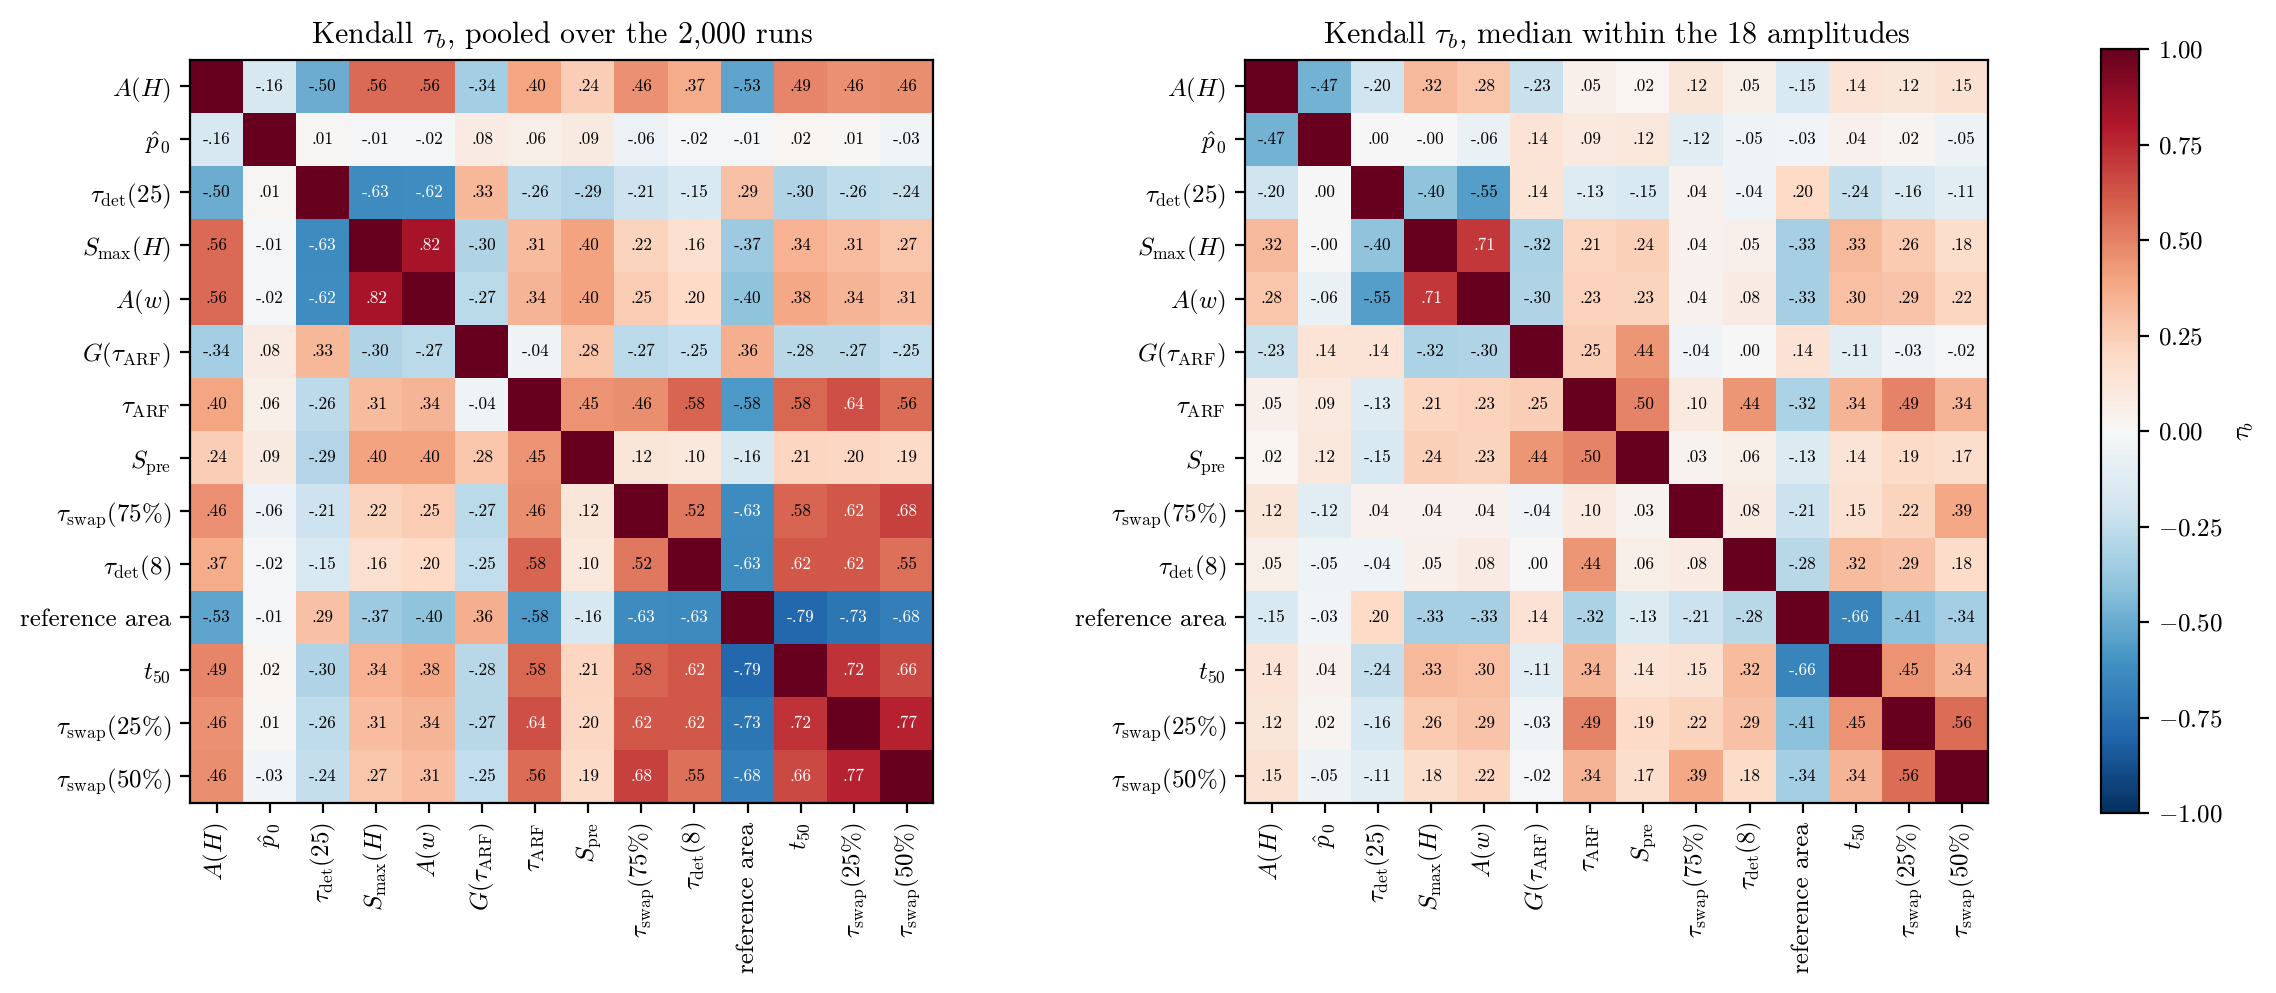
\includegraphics[width=0.86\textwidth]{Fig_QD_matrice_correlations_full.png}
  \end{center}
  \vspace{-0.5em}
  \small
  \begin{columns}[T,onlytextwidth]
    \begin{column}{0.32\textwidth}
      \textbf{Left, pooled:} almost everything agrees, because the drift size moves every
      indicator.
    \end{column}\hfill
    \begin{column}{0.32\textwidth}
      \textbf{Right, within a size:} two groups remain, \emph{evidence} ($0.71$) and
      \emph{repair}, weakly joined.
    \end{column}\hfill
    \begin{column}{0.32\textwidth}
      Best date against the analytic reference: \alert{3 trees replaced}, $0.45$, ahead of
      the first tree, $0.34$.
    \end{column}
  \end{columns}
  \note{Pour voir tous les indicateurs d'un coup, nous en avons croisé quatorze. Le panneau
    de gauche mélange tous les runs : presque tout est fortement corrélé avec tout. C'est une
    illusion, le paradoxe de Simpson : la taille du drift déplace chaque indicateur, donc le
    mélange fabrique de l'accord. Le panneau de droite calcule les mêmes corrélations à
    l'intérieur de chaque taille de drift. L'essentiel de l'accord disparaît, et deux groupes
    subsistent. Un groupe mesure la preuve et les dégâts : le pic du détecteur et l'erreur
    excédentaire sur la transition s'accordent fortement. L'autre groupe mesure la
    réparation. Entre les deux groupes, les liens restent faibles. Nous avons aussi comparé
    les dates de remplacement à une référence analytique, la précision de la forêt sur la
    région dont l'étiquette a changé. La date à laquelle trois arbres sont remplacés la suit
    mieux que le premier arbre. Cette matrice est exploratoire.}
\end{frame}

% =====================================================================
\section{III. Evidence vs threshold}
% =====================================================================

\begin{frame}{Part III --- Evidence against the threshold}
  \begin{center}\carte{3}\end{center}
  \note{La troisième partie relie les deux premières.}
\end{frame}

\begin{frame}{The race is decided before the repair}
  \begin{columns}[c,onlytextwidth]
    \begin{column}{0.52\textwidth}
      \centering
      \resizebox{\linewidth}{!}{\schemaidentite}\\
      {\scriptsize\color{gray} schematic}
    \end{column}\hfill
    \begin{column}{0.44\textwidth}
      A time counts observations; $\lambda$ counts \emph{excess errors}. Comparing them
      needs a rate that does not exist.
      \begin{block}{Race identity, on every run}
        \vspace{-0.4em}
        \[
          \tau_{\mathrm{det}} < \tau_{\mathrm{ARF}}
          \iff S_{\mathrm{pre}} \ge \lambda
        \]
        \vspace{-0.9em}
        \[
          S_{\mathrm{pre}} = \max_{t < \tau_{\mathrm{ARF}}} S_t
        \]
      \end{block}
      \vspace{-0.3em}
      {\scriptsize\color{gray} $S_{\mathrm{pre}}$: the highest the detector's evidence gets
       before the forest repairs itself\par}
      \vspace{0.3em}
      \small No rate, no averaging, no assumption on the trees. Checked on $2\,000$ runs out
      of $2\,000$ at three thresholds.
    \end{column}
  \end{columns}
  \note{Voici l'étape clé. Un temps de réparation compte des observations. Un seuil compte
    des erreurs excédentaires. Ils ne sont pas dans la même unité, et l'article fait le pont
    avec un taux moyen d'erreurs par pas. Ce taux n'existe pas : il chute à mesure que la
    forêt se répare, et le détecteur oublie sa preuve chaque fois qu'il touche zéro.
    L'énoncé exact est bien plus simple. Regardez la statistique du détecteur jusqu'au
    premier remplacement, et prenez son point le plus haut : nous l'appelons S pré. Le
    détecteur arrive premier si et seulement si S pré atteint le seuil. Avec un seuil bas, il
    est atteint avant la réparation ; avec un seuil haut, il ne l'est pas. C'est exact sur
    chaque run, ça ne demande ni taux, ni moyenne, ni hypothèse sur les arbres, et nous
    l'avons vérifié sur les deux mille runs.}
\end{frame}

\begin{frame}{The evidence before the repair sets the transition}
  \begin{columns}[c,onlytextwidth]
    \begin{column}{0.60\textwidth}
      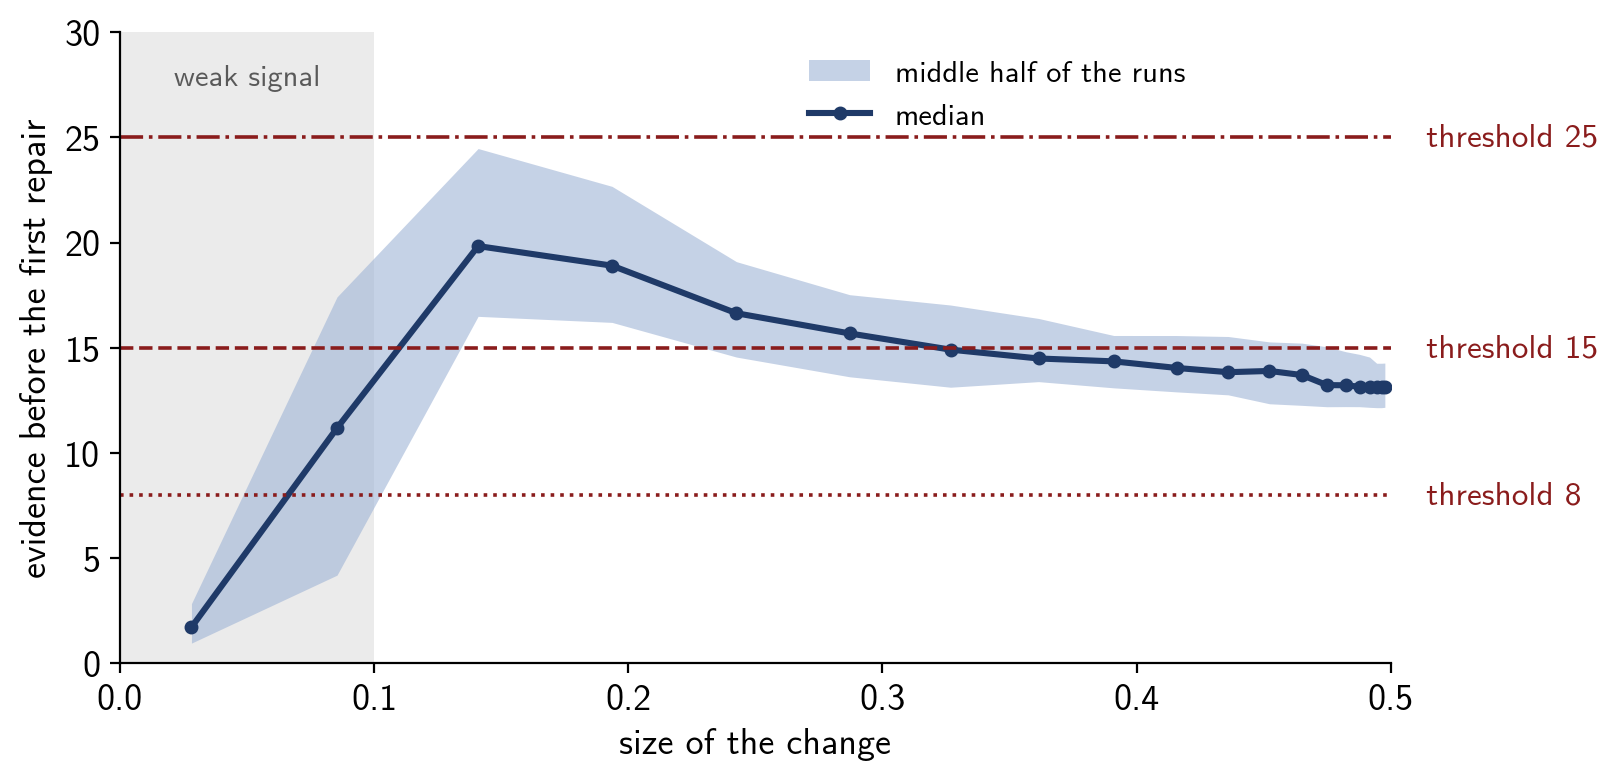
\includegraphics[width=\textwidth]{Fig_slide_spre.png}
    \end{column}\hfill
    \begin{column}{0.37\textwidth}
      \begin{itemize}
        \item Above the weak-signal zone, the median lies between \textbf{$13.1$ and $19.8$}:
              the transition the paper sees between $15$ and $25$, \alert{and leaves
              unexplained}.
        \item It \textbf{decreases} as the drift grows: at $\lambda = 15$ the detector wins
              $81\%$, then only $18\%$. That is the paradox.
      \end{itemize}
    \end{column}
  \end{columns}
  \note{Nous avons donc mesuré S pré sur chaque run. La ligne sombre est la médiane par
    taille de drift, la bande contient la moitié centrale des runs, et les lignes rouges sont
    des seuils. Au-dessus de la zone de signal faible, la médiane se situe entre treize et
    vingt. Un seuil sous ce niveau est atteint avant la réparation dans la plupart des runs ;
    un seuil au-dessus l'est rarement. C'est exactement la transition que l'article observe
    entre quinze et vingt-cinq, et qu'il laisse aux travaux futurs. Regardez maintenant la
    forme. Après les drifts moyens, S pré décroît quand le drift se renforce, parce que le
    premier remplacement vient plus tôt. À seuil fixé à quinze, le détecteur gagne
    quatre-vingt-un pour cent des courses sur les drifts moyens, et seulement dix-huit pour
    cent sur les plus forts. Le paradoxe, c'est cette preuve décroissante, lue face à un
    seuil fixe. Tout à gauche, le drift est trop faible pour accumuler quoi que ce soit :
    c'est un autre régime.}
\end{frame}

\begin{frame}{Stronger drifts leave no more evidence}
  \begin{columns}[c,onlytextwidth]
    \begin{column}{0.48\textwidth}
      \centering
      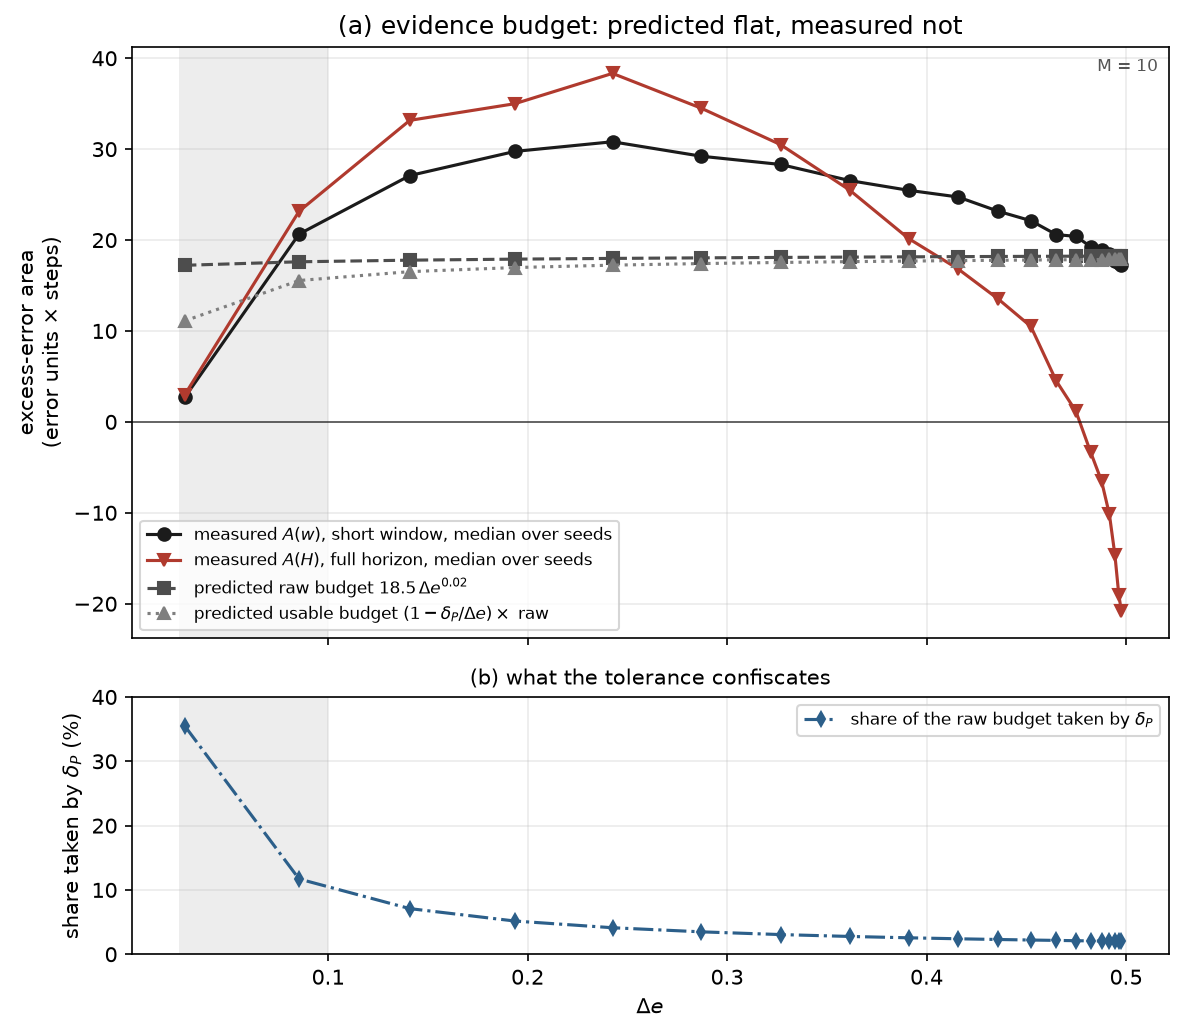
\includegraphics[height=0.66\textheight]{Fig_QC_budget_utilisable_full.png}
    \end{column}\hfill
    \begin{column}{0.46\textwidth}
      \begin{itemize}
        \item The paper's picture: an excess error $\Delta e$ over a window $\tau_{\mathrm{ARF}}$,
              so the area stays almost constant.
        \item Measured over the transition, the area varies by a factor of $1.8$ while the
              drift size varies by $5.8$: \alert{the compensation is real}.
        \item But the paper's rectangle misestimates it by up to $43\%$, and over the whole
              horizon the area turns negative at large drifts: the new task is easier.
      \end{itemize}
    \end{column}
  \end{columns}
  \note{Pourquoi un drift violent ne laisse-t-il pas plus de preuve qu'un drift doux ?
    L'image de l'article est un rectangle : une erreur excédentaire de hauteur delta e,
    pendant une fenêtre égale au temps de réparation. Comme le temps de réparation décroît
    comme un sur delta e, l'aire reste presque constante. Nous avons mesuré l'aire
    directement. Sur la transition, elle varie d'un facteur inférieur à deux, alors que la
    taille du drift varie de presque six : la compensation est réelle. Mais le rectangle
    lui-même est faux. Il se trompe sur l'aire jusqu'à quarante-trois pour cent, parce que le
    premier remplacement n'est pas la largeur du transitoire. Et sur tout l'horizon, aux
    grands drifts, l'aire devient même négative : après le changement, la tâche est plus
    facile qu'avant, et l'erreur se stabilise sous son ancien niveau. La preuve existe, elle
    est à peu près constante, mais la dérivation qu'en fait l'article ne tient pas.}
\end{frame}

\begin{frame}{Detecting is not winning}
  \begin{center}
    \begin{tabular}{@{}cccc@{}}
      \toprule
      threshold $\lambda$ & alarm fires & detector arrives first & false alarms, no drift \\
      \midrule
      $8$  & $95.3\%$ & $\mathbf{91.0\%}$ & $4.15\%$ \\
      $15$ & $92.9\%$ & $\mathbf{36.3\%}$ & $0.15\%$ \\
      $20$ & $66.2\%$ & $8.1\%$           & $0.00\%$ \\
      $25$ & $38.9\%$ & $2.5\%$           & $0.00\%$ \\
      \bottomrule
    \end{tabular}\\[0.3em]
    {\scriptsize\color{gray} $2\,000$ runs with drift and $2\,000$ without, over $2\,000$ steps}
  \end{center}
  \begin{itemize}
    \item At $\lambda = 15$ the alarm almost always fires, but mostly \emph{after} the repair.
    \item At $\lambda = 8$ the detector wins $91\%$ of races for $4.15\%$ of drift-free runs
          with a false alarm: the paper's ``no threshold escapes'' does not hold on this bench.
    \item \textcolor{gray}{Not tested: the heteroscedastic streams where the paper places its
          false-alarm tension.}
  \end{itemize}
  \note{Une conséquence pratique. Détecter un drift et gagner la course sont deux choses
    différentes. Au seuil quinze, l'alarme part sur quatre-vingt-treize pour cent des
    drifts, ce qui paraît excellent, mais elle arrive avant la réparation dans seulement
    trente-six pour cent d'entre eux. La plupart de ces alarmes viennent après que la forêt a
    déjà changé. Au seuil huit, le détecteur gagne quatre-vingt-onze pour cent des courses,
    et environ quatre pour cent des runs où rien ne se passe lèvent une fausse alarme en deux
    mille pas. Au seuil douze, il gagne encore soixante-dix-neuf pour cent des courses, pour
    un demi pour cent de fausses alarmes. Donc sur ce banc, les seuils bas échappent bel et
    bien au point aveugle, et l'affirmation de l'article qu'aucun seuil n'y échappe doit
    être restreinte. Nous n'avons pas testé les flux financiers à volatilité groupée, où
    l'article situe le problème des fausses alarmes.}
\end{frame}

% =====================================================================
\section{Conclusion}
% =====================================================================

\begin{frame}{What changes in the paper}
  \small
  \begin{tabular}{@{}p{0.34\textwidth}p{0.43\textwidth}l@{}}
    \toprule
    The paper & Our result & \\
    \midrule
    races the repair against a constant & race identified, bounded, decided run by run & \textbf{made exact} \\
    independent trees, bias asserted & direction proven, cannot reverse & \textbf{proven} \\
    error back to normal at the first replacement & it comes back later; the rectangle fails & \textbf{corrected} \\
    first replacement as the repair date & earliest date, fires without drift & \textbf{qualified} \\
    transition between $15$ and $25$, unexplained & set by the evidence before the repair & \textbf{explained} \\
    no threshold escapes & $\lambda = 8$ and $12$ do, on this bench & \textbf{restricted} \\
    \bottomrule
  \end{tabular}
  \vspace{0.6em}
  \begin{center}
    \alert{The phenomenon survives. What changes is its mechanism and its reach.}
  \end{center}
  \note{Pour résumer ce que notre travail change dans l'article. La course, qui comparait un
    temps aléatoire à une constante, est rendue exacte : identifiée, bornée, et décidée run
    par run. Le biais de l'hypothèse d'indépendance était affirmé ; il est maintenant
    prouvé, avec son sens. L'idée que l'erreur est revenue à la normale au premier
    remplacement est corrigée. Le premier remplacement comme date de réparation est
    qualifié : c'est la date la plus précoce et elle se déclenche sans drift. Le seuil de
    transition, que l'article laissait inexpliqué, est expliqué par la preuve avant la
    réparation. Et l'affirmation qu'aucun seuil n'échappe est restreinte aux réglages que
    l'article a réellement testés. Le phénomène survit à tout cela. Ce qui change, c'est son
    mécanisme, et sa portée.}
\end{frame}

\begin{frame}{An open question, and what we did not do}
  \begin{columns}[T,onlytextwidth]
    \begin{column}{0.50\textwidth}
      \begin{exampleblock}{Open: a reference for adaptation}
        Every indicator on the detector's side reads the \emph{error}, which mixes what the
        forest relearned with how hard the new task is. On analytic probes, the forest can
        relearn the changed region and lose a rare one, unseen by the error.
      \end{exampleblock}
    \end{column}\hfill
    \begin{column}{0.46\textwidth}
      \begin{block}{Not done}
        \small
        \begin{itemize}
          \item one forest size, one homoscedastic bench
          \item decision rule fixed during the analysis
          \item the independence bias has a sign, not a size
        \end{itemize}
      \end{block}
    \end{column}
  \end{columns}
  \note{Nous laissons une question ouverte. Toute mesure disponible pour le détecteur lit
    l'erreur, et l'erreur mélange deux choses : ce que la forêt a réappris, et la difficulté
    de la nouvelle tâche. Avec des sondes analytiques, des points dont nous connaissons la
    vraie étiquette, nous avons vu que la forêt peut réapprendre la région qui a changé tout
    en perdant une région rare ailleurs, et l'erreur ne voit pas cette perte. Alors quelle
    serait une vraie référence pour l'adaptation ? Nous n'avons pas la réponse. Et pour être
    honnêtes sur les limites : nous avons étudié une seule taille de forêt sur un seul banc
    simple, notre règle de décision a été fixée pendant l'analyse plutôt qu'avant, et nous
    pouvons donner le signe du biais d'indépendance mais pas sa taille.}
\end{frame}

\begin{frame}{Take-away}
  \begin{center}
    \small\alert{The blind spot is a budget of evidence, accumulated before the repair, set
    against a threshold.}
  \end{center}
  \vspace{-0.5em}
  \begin{center}\carte[0.71]{0}\end{center}
  \note{Retour à la carte. Le point aveugle est réel, et il survit à toutes les corrections.
    Mais ce n'est pas une course entre deux horloges. C'est la preuve que la forêt laisse
    passer avant sa première réparation, face à un seuil fixe. Cette seule grandeur explique
    quand le détecteur gagne, pourquoi la transition est là où elle est, et pourquoi les
    drifts plus forts sont ratés plus souvent. Merci de votre attention ; nous sommes à votre
    disposition pour vos questions.}
\end{frame}

% =====================================================================
\appendix
\section*{Backup}
% =====================================================================

\begin{frame}{Backup --- The supervisor's additional questions}
  {\small Treated in a separate working document on the same campaign; not merged into the report.}
  \begin{itemize}
    \item \textbf{Shape of the error after the drift}: not exponential, and its half-recovery comes
          \emph{after} the median first replacement on $17$ of the $18$ readable drift sizes.
          The first replacement is early, again.
    \item \textbf{End of the horizon}: the error settles \emph{below} its pre-drift baseline at all
          $20$ drift sizes. The new task is easier.
    \item \textbf{Inside the forest} (pilot, $100$ runs): disagreement between trees halves when only
          $63$ to $66\%$ of them are renewed --- the surviving trees learn too. After a strong drift,
          new trees err far less than survivors.
    \item \textbf{A z-score of the error drop} measures the number of seeds, not the dynamics.
  \end{itemize}
  \vfill
  {\small\color{gray} Open, and worth continuing: a reference for adaptation, the size of the
  independence bias, heteroscedastic streams, tree-by-tree dynamics.}
\end{frame}

\begin{frame}{Backup --- Fréchet bounds}
  For integer-valued clocks with marginal CDFs $F_A$ and $F_D$, and \emph{any} coupling,
  \begin{align*}
    P_{\mathrm{miss}} &\ge \max\Big(0,\ \sup_{s} \big[F_A(s)-F_D(s)\big]\Big),\\
    P_{\mathrm{miss}} &\le \min\Big(1,\ \inf_{s} \big[F_A(s) + 1 - F_D(s+1)\big]\Big).
  \end{align*}
  \begin{itemize}
    \item Lower: Fréchet on $\{\tau_{\mathrm{ARF}} \le s < \tau_{\mathrm{det}}\} \subseteq \mathrm{Miss}$.
    \item Upper: $\mathrm{Miss} \subseteq \{\tau_{\mathrm{ARF}} \le s\} \cup \{\tau_{\mathrm{det}} > s+1\}$, then Boole.
    \item Toy case, both clocks uniform on $\{1,2\}$: the bounds $0$ and $0.5$ are both attained.
  \end{itemize}
\end{frame}

\begin{frame}{Backup --- Lindley's closed form and the certificate}
  With $X_t = e_t - \hat p_0 - \delta_P$ and $A(k,j) = \sum_{t=k+1}^{j} (e_t - \hat p_0)$,
  \[
    S_j = \max_{0 \le k \le j} \sum_{t=k+1}^{j} X_t,
    \qquad
    S_{\max}(H) = \max_{0 \le k \le j \le H} \big[A(k,j) - (j-k)\,\delta_P\big].
  \]
  \begin{itemize}
    \item Certificate: the alarm fires by $H$ iff some sub-window carries
          $A(k,j) \ge \lambda + (j-k)\,\delta_P$. The full window alone is only sufficient.
    \item Race identity: the same maximum, taken up to the first replacement, is $S_{\mathrm{pre}}$.
  \end{itemize}
\end{frame}

\begin{frame}{Backup --- Association protocol}
  \begin{itemize}
    \item Every coefficient is computed \textbf{within a drift size} ($100$ seeds), on the $18$
          sizes with $\Delta e \ge 0.10$: pooling measures the drift size, not the link.
    \item Kendall's $\tau_b$: reads on pairs, corrects for ties. Censored durations ranked last,
          licit because the horizon is common to all runs.
    \item Pearson undefined on censored values; Spearman handles their ties implicitly.
    \item Percentile bootstrap over seeds, $2\,000$ resamples; discernible if the interval
          excludes zero. Fixed during the analysis, not before: stated in the report.
    \item Complete cases instead of ranking censored runs last: no coefficient moves by more
          than $0.0403$.
  \end{itemize}
\end{frame}

\begin{frame}{Backup --- The drift-free control}
  \begin{center}
    \begin{tabular}{@{}lr@{}}
      \toprule
      On $2\,000$ runs with no change point & \\
      \midrule
      runs where at least one tree is replaced & $2\,000/2\,000$ \\
      first replacement, median & $95$ steps \\
      distinct trees renewed, median & $9/10$ \\
      forest entirely renewed & $28.7\%$ \\
      \midrule
      first replacement at the weakest drift, median & $118$ steps \\
      \bottomrule
    \end{tabular}
  \end{center}
\end{frame}

\begin{frame}{Backup --- Notation}
  \begin{center}
    \small
    \begin{tabular}{@{}ll@{}}
      \toprule
      $\Delta e$ & drift size: the jump in error a stale model suffers \\
      $\tau_{\mathrm{ARF}}$ & first tree replaced after the change \\
      $\tau_{\mathrm{swap}}(q)$ & first time a share $q$ of the trees has been replaced \\
      $\tau_{\mathrm{det}}$ & first alarm of the external detector, possibly never \\
      $S_t$, $\lambda$ & detector statistic and its threshold \\
      $S_{\mathrm{pre}}$ & highest $S_t$ reached before the first replacement \\
      $A(w)$, $A(H)$ & excess error over the transient window, over the whole horizon \\
      $G$ & share of the detector's final evidence already reached at $\tau_{\mathrm{ARF}}$ \\
      \bottomrule
    \end{tabular}
  \end{center}
\end{frame}

\end{document}
"
% soutenance_20min.tex
% =====================================================================
% Soutenance du 16/09/2026 : 20 minutes de presentation, 10 de questions.
%
% Trame : celle du rapport refondu. These : le point aveugle n'est pas une
% course entre deux horloges mais un budget de preuve contre un seuil. La
% carte des idees (soutenance_schemas.tex) ouvre le propos, revient en tete
% de chaque partie avec la partie en couleur, et le conclut.
%
% Consignes de l'encadrant : vue globale, concepts, resultats inattendus ;
% pas de details de preuve, de calcul ou d'implementation dans le corps.
% Les preuves et le protocole sont en slides de secours, apres la fin.
% Pas de renvoi aux numeros de questions du sujet (preference du groupe).
%
% Duree : les notes sont le texte parle, environ 2 600 mots, soit
% 20 minutes a 130 mots par minute.
%
% Style : Madrid, comme le pitch. Compilation : lualatex, deux passes.
% Notes seules : lualatex -jobname=soutenance_notes "\def\NOTESSEULES{}% soutenance_20min.tex
% =====================================================================
% Soutenance du 16/09/2026 : 20 minutes de presentation, 10 de questions.
%
% Trame : celle du rapport refondu. These : le point aveugle n'est pas une
% course entre deux horloges mais un budget de preuve contre un seuil. La
% carte des idees (soutenance_schemas.tex) ouvre le propos, revient en tete
% de chaque partie avec la partie en couleur, et le conclut.
%
% Consignes de l'encadrant : vue globale, concepts, resultats inattendus ;
% pas de details de preuve, de calcul ou d'implementation dans le corps.
% Les preuves et le protocole sont en slides de secours, apres la fin.
% Pas de renvoi aux numeros de questions du sujet (preference du groupe).
%
% Duree : les notes sont le texte parle, environ 2 600 mots, soit
% 20 minutes a 130 mots par minute.
%
% Style : Madrid, comme le pitch. Compilation : lualatex, deux passes.
% Notes seules : lualatex -jobname=soutenance_notes "\def\NOTESSEULES{}\input{soutenance_20min}"
%
% Tracabilite : chaque chiffre vient du rapport ; controle par
%   verif_chiffres_tex.py ../../05_presentation/soutenance_20min.tex
% Figures : figures_slides.py --latex, figures_soutenance.py,
%   matrice_correlations.py, analyse_QCD.py (budget).
% =====================================================================

\documentclass[aspectratio=169,11pt]{beamer}

\usetheme{Madrid}
% Rouge de CentraleSupelec, pris dans le logo officiel (#B00739) ; logo
% CentraleSupelec / Universite Paris-Saclay sur la page de titre.
\definecolor{csRouge}{HTML}{B00739}
\usecolortheme[named=csRouge]{structure}
\setbeamercolor{alerted text}{fg=csRouge}
\setbeamersize{text margin left=1cm, text margin right=1cm}
\setbeamertemplate{navigation symbols}{}
\usepackage[english]{babel}
\usepackage{amsmath,amssymb}
\usepackage{graphicx}
\usepackage{booktabs}
\usepackage{tikz}
\input{soutenance_schemas}
\titlegraphic{
\includegraphics[height=1.7cm]{Logo_CS_Paris_Saclay.png}}
\ifdefined\NOTESSEULES\setbeameroption{show only notes}\fi
\graphicspath{{../04_experimentations/resultats_R2/resultats/figures/slides_latex/}{../04_experimentations/resultats_R2/resultats/figures/}}

\setbeamerfont{author}{size=\small}
\setbeamerfont{institute}{size=\scriptsize}

\title[The Blind Spot Paradox]{The Blind Spot Paradox}
\subtitle{Formalizing the race and measuring the adaptation}
\author[Boyer, Gouillou, Fonvielle, Petit-Tichanné]{Alexandre Boyer \and Melaine Gouillou \and Salomé Fonvielle \and Ulysse Petit-Tichanné}
\institute[CS]{Research Track, Topic 39, CentraleSupélec. Supervisor: Raphaël Minato}
\date{16 September 2026}

\begin{document}

\maketitle
\note{Good afternoon. Our subject is the blind spot paradox: a model that repairs
  itself can destroy the very evidence its own monitor needs. In the next twenty
  minutes we will present what we formalized, what we measured, and the single
  reading that ties the two together.}

% =====================================================================
\section{The problem}
% =====================================================================

\begin{frame}{Concept drift: the rule changes, the data does not}
  \vspace{-0.6em}
  \[
    \underbrace{P(X)}_{\text{the data}}\ \text{unchanged}
    \qquad\qquad
    \underbrace{P(Y \mid X)}_{\text{the rule}}\ \text{changes}
  \]
  \vspace{-0.9em}
  \begin{center}
    
\includegraphics[height=0.50\textheight]{Fig_slide_drift.png}
  \end{center}
  \begin{center}
    A model trained before the change is now \alert{wrong on the shaded band}.
  \end{center}
  \note{A classifier learns a rule from data. In a data stream, that rule can change
    while the inputs keep exactly the same distribution. This is concept drift: P of X
    does not move, P of Y given X does. It is the normal situation for a financial
    signal, where the same inputs stop meaning the same thing. In the bench we use,
    points in the plane are separated by a line. At the change, the line moves. Every
    point in the shaded band switches label, so a model trained before the change keeps
    predicting confidently, and is now wrong on that band. The size of the band is the
    size of the drift, written delta e.}
\end{frame}

\begin{frame}{Two defences that run at the same time}
  \begin{columns}[T,onlytextwidth]
    \begin{column}{0.49\textwidth}
      \centering
      \textbf{The model repairs itself}\\[0.3em]
      
\includegraphics[width=\textwidth]{Fig_slide_foret.png}\\[0.2em]
      \small Adaptive Random Forest: ten trees, each replaced when its own error rises.
    \end{column}\hfill
    \begin{column}{0.49\textwidth}
      \centering
      \textbf{A monitor raises the alarm}\\[0.3em]
      
\includegraphics[width=\textwidth]{Fig_slide_watchdog.png}\\[0.2em]
      \small Each error adds to a statistic $S_t$; the alarm fires when it crosses $\lambda$.
    \end{column}
  \end{columns}
  \note{Two defences are deployed together. The first one lives inside the model. The
    Adaptive Random Forest is made of ten decision trees that vote. Each tree watches its
    own error with a small detector, and when that error rises, the tree is replaced by a
    fresh one. The forest repairs itself locally, without asking anyone. The second defence
    sits outside. A cumulative detector, a Page-Hinkley test, watches the error of the
    whole forest. Every error pushes a statistic up by almost one, every correct answer
    pulls it down a little, never below zero. When the statistic crosses a threshold
    lambda, the alarm fires, and that alarm is the only thing a human operator sees.}
\end{frame}

\begin{frame}{The paradox, and what the reviewers asked}
  \begin{columns}[c,onlytextwidth]
    \begin{column}{0.50\textwidth}
      \centering
      
\includegraphics[width=\textwidth]{Fig_slide_mecanisme.png}\\
      {\scriptsize\color{gray} schematic}
    \end{column}\hfill
    \begin{column}{0.46\textwidth}
      \begin{block}{The paper's claim}
        The stronger the drift, the faster the repair, and the \alert{fewer} alarms.
      \end{block}
      \begin{alertblock}{Two corrections requested}
        \begin{enumerate}
          \item It races a random repair time against a \emph{constant}, and assumes the
                trees independent.
          \item It dates the repair at the \emph{first} tree replaced, without showing
                that this date means anything.
        \end{enumerate}
      \end{alertblock}
    \end{column}
  \end{columns}
  \note{When both defences run together, something unexpected happens. The drift starts,
    errors pile up in the detector, but the forest replaces trees, the errors stop, and the
    pile drains before it reaches the threshold. The paper we study calls this the blind
    spot paradox: the stronger the drift, the faster the forest repairs itself, and the
    fewer alarms the operator gets. The paper was reviewed, and two corrections were
    requested. First, it compares a random repair time with a constant detection time, and
    it assumes the ten trees are independent without proving it. Second, it dates the repair
    at the moment the first tree is replaced, without showing that this moment has anything
    to do with the error disappearing. These two corrections are where our work starts.}
\end{frame}

\begin{frame}{Our reading, in one map}
  \begin{center}
    \small\alert{The blind spot is not a race between two clocks,
    but a budget of evidence set against a threshold.}
  \end{center}
  \vspace{-0.5em}
  \begin{center}
    \carte[0.71]{0}
  \end{center}
  \note{Here is the whole talk on one map. At the top, the claim of the paper. The first
    column formalizes the race: we define the blind spot properly, we compute its
    probability, and we show that assuming independent trees makes the paper optimistic
    about the repair. The second column asks what the repair date really measures: it is
    the earliest possible date, it fires even when nothing changes, and when it fires most
    of the evidence is already there. The third column ties both together: the detector wins
    exactly when its evidence reaches the threshold before the repair, and that evidence
    explains both the transition and the paradox. The dashed arrows are the links between
    columns, and the box at the bottom is the question we leave open. Our one-sentence
    reading: the blind spot is not a race between two clocks, it is a budget of evidence set
    against a threshold.}
\end{frame}

% =====================================================================
\section{I. The race}
% =====================================================================

\begin{frame}{Part I --- The race, formally}
  \begin{center}\carte{1}\end{center}
  \note{Let us start with the theory: how to state the race without cheating.}
\end{frame}

\begin{frame}{The race is well posed, and its probability identified}
  \begin{columns}[T,onlytextwidth]
    \begin{column}{0.46\textwidth}
      \begin{block}{One definition, no ad hoc rule}
        \[
          \mathrm{Miss} := \{\tau_{\mathrm{ARF}} < \tau_{\mathrm{det}}\}
        \]
        \vspace{-0.6em}
        {\small strict inequality; the alarm may never come}
        \begin{itemize}
          \item a tie goes to the detector
          \item a silent repair, with no alarm ever, \alert{is} a miss
          \item if neither acts, it is not
        \end{itemize}
      \end{block}
    \end{column}\hfill
    \begin{column}{0.50\textwidth}
      \begin{exampleblock}{What the campaign allows}
        The forest always replaces a tree within the horizon, so no run is left
        undecided: $P_{\mathrm{miss}}$ is \textbf{identified}.\\[0.3em]
        \centering
        \begin{tabular}{@{}lccc@{}}
          $\lambda$ & $8$ & $25$ & $50$ \\
          $P_{\mathrm{miss}}$ & $0.0905$ & $0.9715$ & $1.0000$
        \end{tabular}
      \end{exampleblock}
      \begin{alertblock}{Without any dependence assumption}
        From the marginal laws alone, the blind spot at the weakest drift is at least
        $0.91$ at $\lambda = 8$.
      \end{alertblock}
    \end{column}
  \end{columns}
  \note{The paper says there is a blind spot when the forest repairs before the alarm, but
    it quietly sets aside the runs where the alarm never comes. Those are exactly the runs
    where the detector fails most. So we define the event on the complete race, with one
    definition and no extra rule. A tie counts for the detector, because the operator is
    warned at the right moment. A silent repair, where the alarm never comes, is a miss, and
    in fact the purest one. A run where neither mechanism acts is not a miss, because there
    was nothing to erase. Then comes the problem of the finite horizon: some runs could be
    undecided. On our campaign they are not, because the forest always acts within the
    horizon, so the miss probability is identified exactly: nine percent at threshold eight,
    ninety-seven at twenty-five, one hundred at fifty. And with Fréchet bounds, which use the
    two marginal laws and assume nothing on how the clocks are coupled, the blind spot at the
    weakest drift is already forced above ninety percent.}
\end{frame}

\begin{frame}{Trees share a stream: the paper is optimistic}
  \begin{enumerate}
    \item \textbf{Given the stream}, what separates two trees is their own random draws:
          the trees are independent \emph{conditionally}.
    \item \textbf{Averaging over streams}, convexity gives the direction:
          \[
            P(\tau_{\mathrm{ARF}} \le s) \;\le\; 1 - \big(1 - F(s)\big)^M
          \]
          \alert{The independence formula overstates the speed of the repair.}
    \item \textbf{Consequence}: the paper's critical ensemble size becomes a conservative
          ceiling; its verdict does not change.
    \item \textbf{No coupling reverses the sign}: sharing a stream can only make trees fail
          together, since the covariance equals a variance.
  \end{enumerate}
  \note{The second shortcut is independence. The ten trees learn from the same stream, so
    they cannot be independent. But the question is at which level. Once the stream is
    fixed, what distinguishes one tree from another is only its own randomness, the random
    weights of online bagging. At that level, given the stream, the trees are independent.
    When we average over streams, Jensen's inequality gives a clear direction: the
    probability that the forest has already repaired itself is at most what the independence
    formula predicts. So the paper makes the forest look faster than it is, and overestimates
    the blind spot. Its critical ensemble size is not wrong, it becomes a conservative
    ceiling, and the paper's own verdict does not change. Could dependence go the other way?
    No: the covariance between two trees equals a variance, so it is never negative.}
\end{frame}

% =====================================================================
\section{II. The repair date}
% =====================================================================

\begin{frame}{Part II --- What the repair date measures}
  \begin{center}\carte{2}\end{center}
  \note{Now the second correction: the date the paper uses for the repair.}
\end{frame}

\begin{frame}{How we measured}
  \begin{columns}[T,onlytextwidth]
    \begin{column}{0.48\textwidth}
      \begin{block}{The campaign}
        \begin{itemize}
          \item the paper's bench, rerun: $20$ drift sizes $\times$ $100$ seeds,
                $2\,000$ steps after the change
          \item $2\,000$ more runs with no change at all
          \item only the error and the replacement events are recorded; every threshold is
                replayed offline
        \end{itemize}
      \end{block}
    \end{column}\hfill
    \begin{column}{0.48\textwidth}
      \begin{block}{Reading an association}
        \begin{itemize}
          \item always \alert{within one drift size}: pooling measures the drift size, not
                the link
          \item Kendall's rank correlation, with bootstrap intervals over the seeds
          \item steps added after seeing the data are flagged as exploratory
        \end{itemize}
      \end{block}
    \end{column}
  \end{columns}
  \note{A word on how we measured, without the implementation details. We reran the bench
    of the paper on twenty drift sizes, with one hundred seeds each, and we observe two
    thousand steps after the change. We added two thousand runs where nothing changes at
    all, as a control. The simulation records only two things: the error at each step and
    the moments when trees are replaced. Everything else, including the detector at any
    threshold, is recomputed offline, so one campaign replaces many. When we correlate two
    quantities, we always do it within one drift size. The drift size moves every indicator
    at once, so a correlation pooled over sizes mostly measures the size itself. We use
    Kendall's rank correlation with bootstrap intervals, and we flag the steps we added
    after looking at the data.}
\end{frame}

\begin{frame}{The first replacement is the earliest possible date}
  \begin{center}
    
\includegraphics[width=0.90\textwidth]{Fig_slide_deux_horloges.png}
  \end{center}
  \vspace{-0.3em}
  \begin{itemize}
    \item On every run, the first replacement comes before any other quota of renewed
          trees. Three quarters of the forest are renewed \textbf{$6.0$ to $14.3$ times later}.
    \item \alert{With no drift at all}, the first replacement comes after $95$ steps in
          median, against $118$ on the weakest drift.
  \end{itemize}
  \note{The paper dates the repair at the first replaced tree. By construction, that is the
    earliest of all possible dates: the moment when three trees, or half, or three quarters
    of the forest are replaced, always comes later, on every run. The only question is how
    much later. On this medium drift, the first tree goes after eighty-six observations, and
    three quarters of the forest after more than twelve hundred. Over the grid, three
    quarters of the forest are renewed six to fourteen times later than the first tree. And
    there is a more worrying fact. On the two thousand runs with no change at all, the forest
    still replaces its first tree, after ninety-five steps in median. On the weakest real
    drift, it takes one hundred and eighteen. So at low drift, this date cannot tell a real
    change from noise.}
\end{frame}

\begin{frame}{When the first tree goes, most of the evidence is already there}
  \begin{columns}[T,onlytextwidth]
    \begin{column}{0.36\textwidth}
      \begin{block}{Evidence at the first replacement}
        \centering
        {\Large $49\%$ to $76\%$}\\[0.2em]
        \small of the detector's final peak, on the $18$ drift sizes studied
      \end{block}
    \end{column}\hfill
    \begin{column}{0.60\textwidth}
      \begin{block}{Does the date track anything, within a drift size?}
        \small
        \begin{tabular}{@{}lcc@{}}
          \toprule
          compared with & median link & sizes \\
          \midrule
          detector peak & $0.21$ & $15/18$ \\
          excess error, whole horizon & none & $0/18$ \\
          excess error, transition only & $0.23$ & $13/18$ \\
          \bottomrule
        \end{tabular}
      \end{block}
    \end{column}
  \end{columns}
  \vspace{0.8em}
  \begin{center}
    \small The null over the whole horizon is mostly noise: \alert{half} of that area's
    variance comes from the estimated baseline, multiplied by the horizon.
  \end{center}
  \note{Is the first replacement at least the end of the transient? No. When the first tree
    is replaced, the detector already holds between half and three quarters of all the
    evidence it will ever accumulate. The replacement is in the middle of the story, not at
    its end. Then we asked whether this date tracks anything, always within a drift size.
    With the peak of the detector, there is a weak but real link, visible on fifteen drift
    sizes out of eighteen. With the excess error over the whole horizon, there is no link at
    all. But we found out why: that area adds up two thousand steps, so any error on the
    baseline is multiplied by two thousand, and half of its variance is just that noise. If
    we keep only the transition, the link comes back, weak but real, on thirteen sizes out of
    eighteen. This last step is exploratory.}
\end{frame}

\begin{frame}{Unexpected: pooling manufactures agreement}
  \begin{center}
    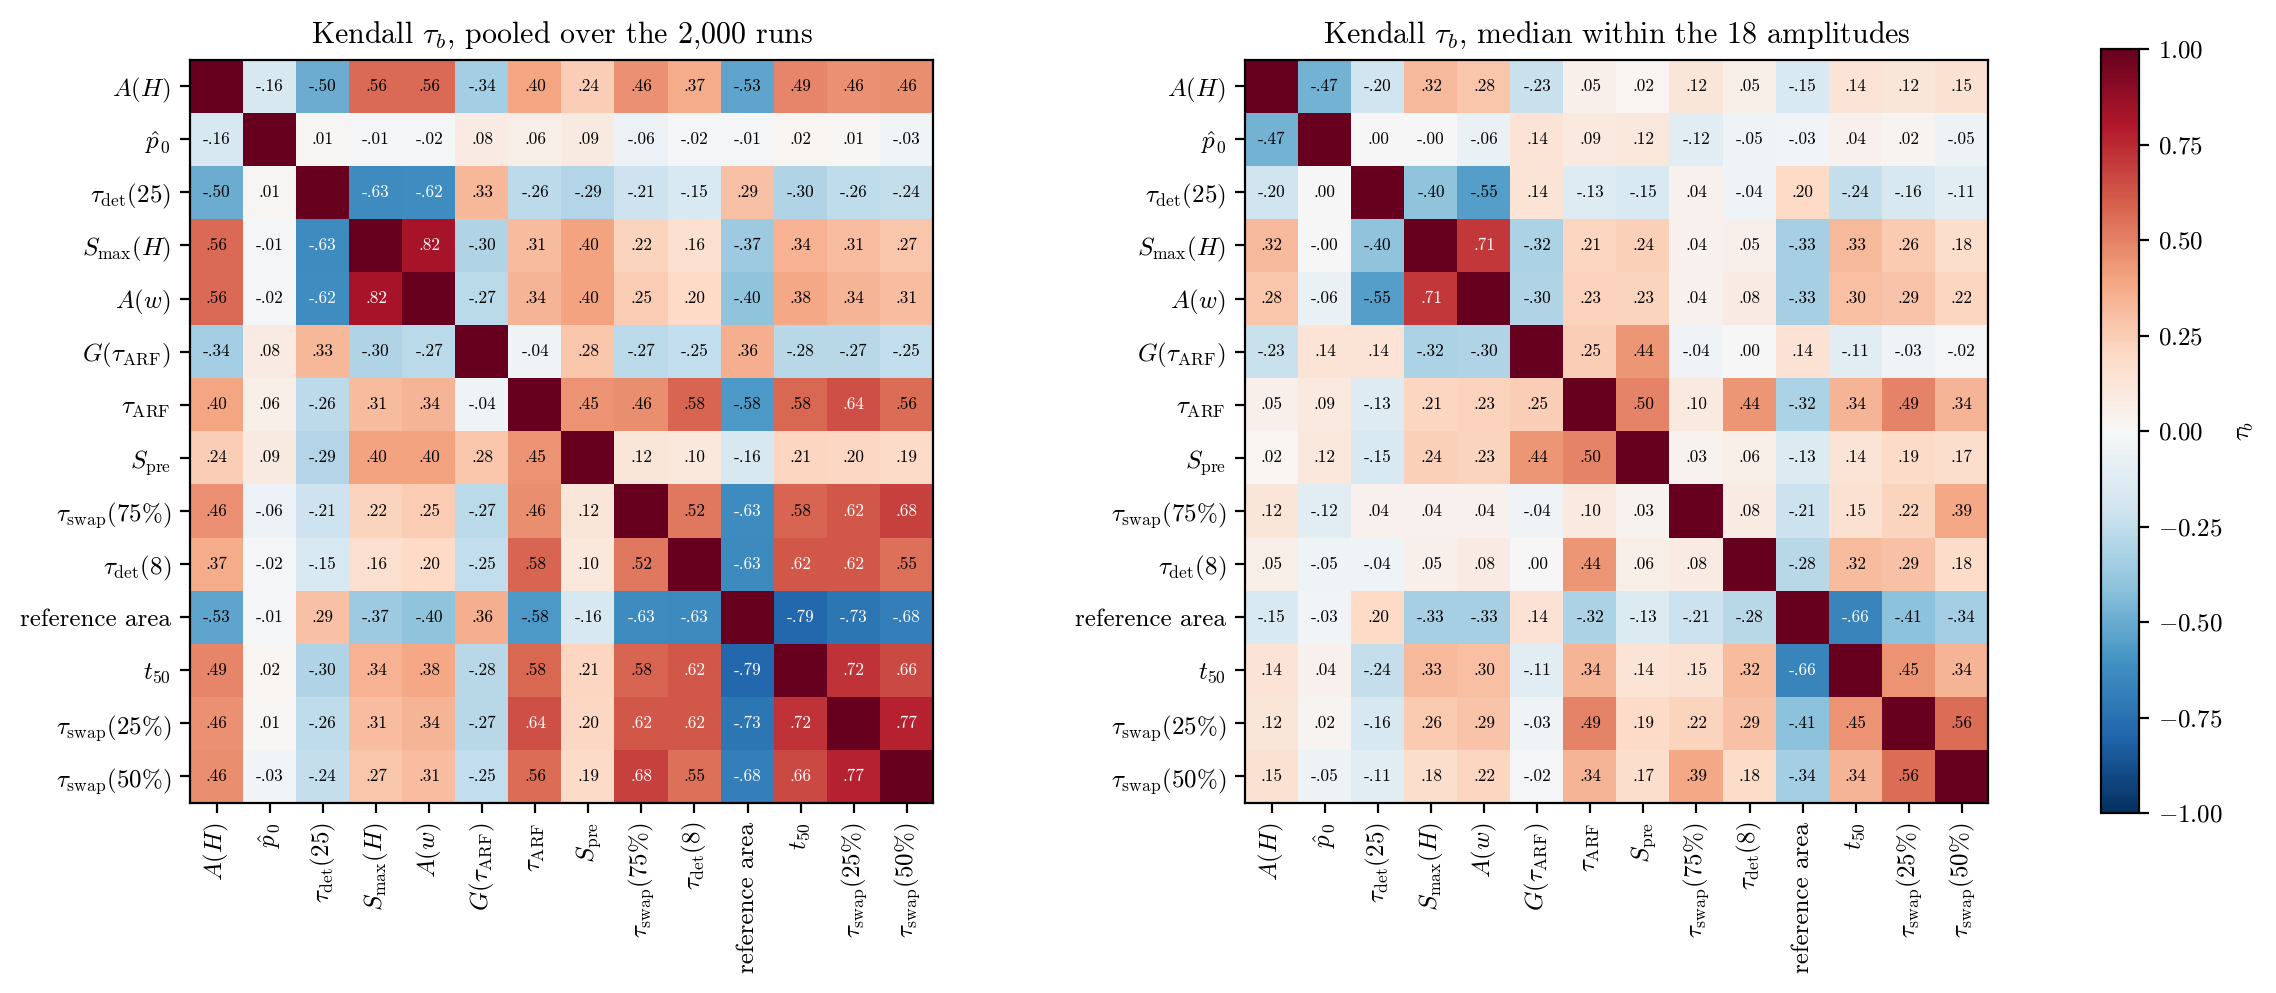
\includegraphics[width=0.86\textwidth]{Fig_QD_matrice_correlations_full.png}
  \end{center}
  \vspace{-0.5em}
  \small
  \begin{columns}[T,onlytextwidth]
    \begin{column}{0.32\textwidth}
      \textbf{Left, pooled:} almost everything agrees, because the drift size moves every
      indicator.
    \end{column}\hfill
    \begin{column}{0.32\textwidth}
      \textbf{Right, within a size:} two groups remain, \emph{evidence} ($0.71$) and
      \emph{repair}, weakly joined.
    \end{column}\hfill
    \begin{column}{0.32\textwidth}
      Best date against the analytic reference: \alert{3 trees replaced}, $0.45$, ahead of
      the first tree, $0.34$.
    \end{column}
  \end{columns}
  \note{To see all indicators at once, we crossed fourteen of them. The left panel pools all
    runs together: almost everything is strongly correlated with everything. That is an
    illusion, Simpson's paradox: the drift size moves every indicator, so pooling creates
    agreement. The right panel computes the same correlations within each drift size. Most of
    the agreement disappears, and two groups remain. One group measures evidence and damage:
    the detector's peak and the excess error over the transition agree strongly. The other
    group measures the repair. Between the two groups, links stay weak. We also compared the
    replacement dates with an analytic reference, the accuracy of the forest on the region
    whose label changed. The date at which three trees are replaced tracks it better than the
    first tree. This matrix is exploratory.}
\end{frame}

% =====================================================================
\section{III. Evidence vs threshold}
% =====================================================================

\begin{frame}{Part III --- Evidence against the threshold}
  \begin{center}\carte{3}\end{center}
  \note{The third part ties the first two together.}
\end{frame}

\begin{frame}{The race is decided before the repair}
  \begin{columns}[c,onlytextwidth]
    \begin{column}{0.52\textwidth}
      \centering
      \resizebox{\linewidth}{!}{\schemaidentite}\\
      {\scriptsize\color{gray} schematic}
    \end{column}\hfill
    \begin{column}{0.44\textwidth}
      A time counts observations; $\lambda$ counts \emph{excess errors}. Comparing them
      needs a rate that does not exist.
      \begin{block}{Race identity, on every run}
        \vspace{-0.4em}
        \[
          \tau_{\mathrm{det}} < \tau_{\mathrm{ARF}}
          \iff S_{\mathrm{pre}} \ge \lambda
        \]
        \vspace{-0.9em}
        \[
          S_{\mathrm{pre}} = \max_{t < \tau_{\mathrm{ARF}}} S_t
        \]
      \end{block}
      \small No rate, no averaging, no assumption on the trees. Checked on $2\,000$ runs out
      of $2\,000$ at three thresholds.
    \end{column}
  \end{columns}
  \note{Here is the key step. A repair time counts observations. A threshold counts excess
    errors. They are not in the same unit, and the paper bridges them with an average rate of
    errors per step. That rate does not exist: it falls as the forest repairs, and the
    detector forgets its evidence each time it hits zero. The exact statement is much
    simpler. Look at the statistic of the detector up to the first replacement, and take its
    highest point: we call it S pre. The detector arrives first if and only if S pre reaches
    the threshold. With a low threshold, it is reached before the repair; with a high one, it
    is not. This is exact on every run, it needs no rate, no averaging and no assumption on
    the trees, and we checked it on all two thousand runs.}
\end{frame}

\begin{frame}{The evidence before the repair sets the transition}
  \begin{columns}[c,onlytextwidth]
    \begin{column}{0.60\textwidth}
      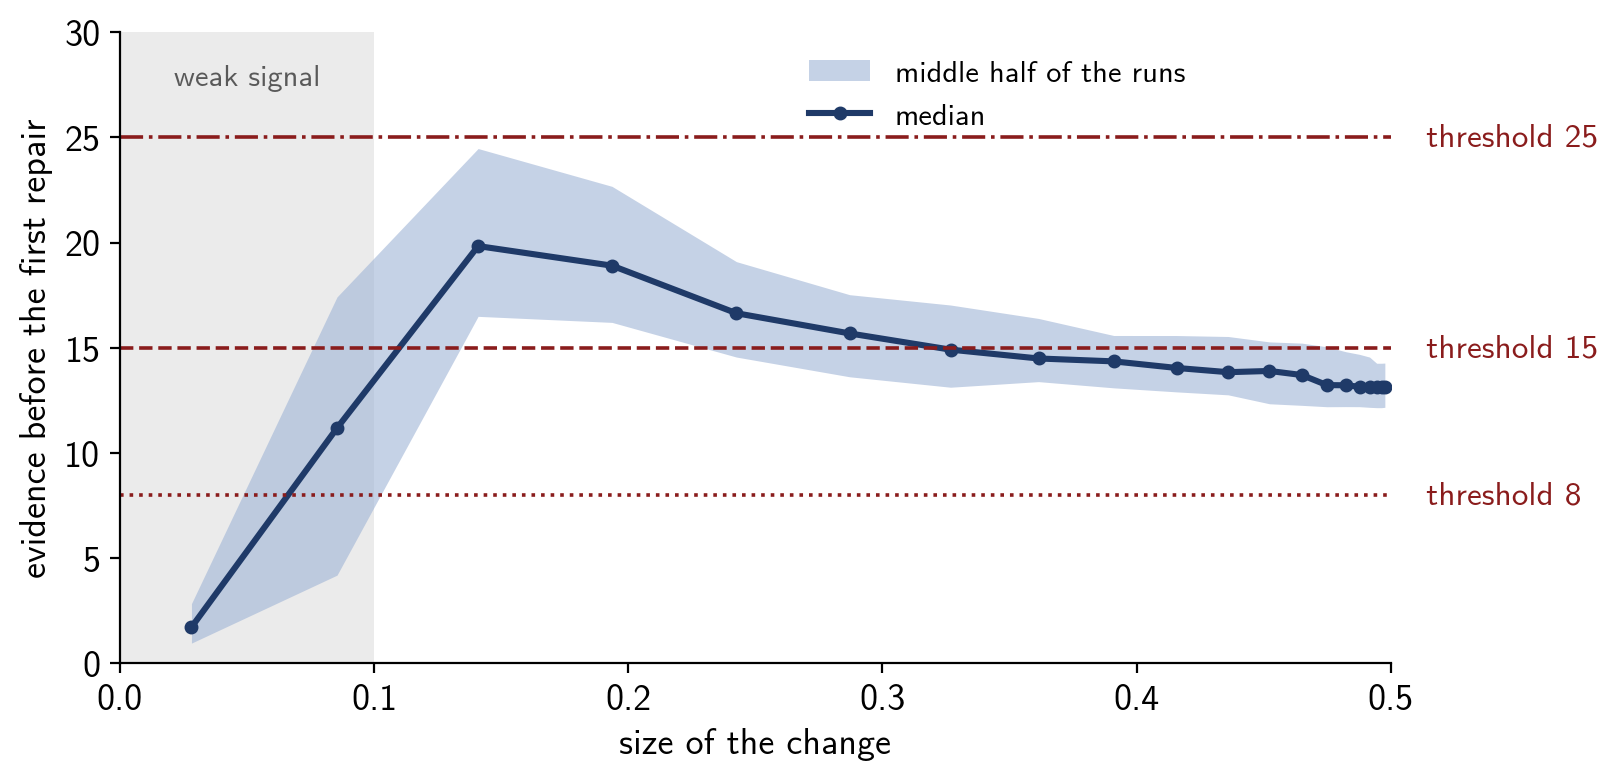
\includegraphics[width=\textwidth]{Fig_slide_spre.png}
    \end{column}\hfill
    \begin{column}{0.37\textwidth}
      \begin{itemize}
        \item Above the weak-signal zone, the median lies between \textbf{$13.1$ and $19.8$}:
              the transition the paper sees between $15$ and $25$, \alert{and leaves
              unexplained}.
        \item It \textbf{decreases} as the drift grows: at $\lambda = 15$ the detector wins
              $81\%$, then only $18\%$. That is the paradox.
      \end{itemize}
    \end{column}
  \end{columns}
  \note{So we measured S pre on every run. The dark line is the median by drift size, the band
    holds the middle half of the runs, and the red lines are thresholds. Above the weak-signal
    zone, the median sits between thirteen and twenty. A threshold below that level is reached
    before the repair in most runs; a threshold above it rarely is. That is exactly the
    transition the paper observes between fifteen and twenty-five, and leaves to future work.
    Now look at the shape. After the medium drifts, S pre decreases as the drift gets stronger,
    because the first replacement comes sooner. At a fixed threshold of fifteen, the detector
    wins eighty-one percent of the races on medium drifts, and only eighteen percent on the
    strongest ones. The paradox is this decreasing evidence, read against a fixed threshold. At
    the far left, the drift is too weak to accumulate anything: that is a different regime.}
\end{frame}

\begin{frame}{Stronger drifts leave no more evidence}
  \begin{columns}[c,onlytextwidth]
    \begin{column}{0.48\textwidth}
      \centering
      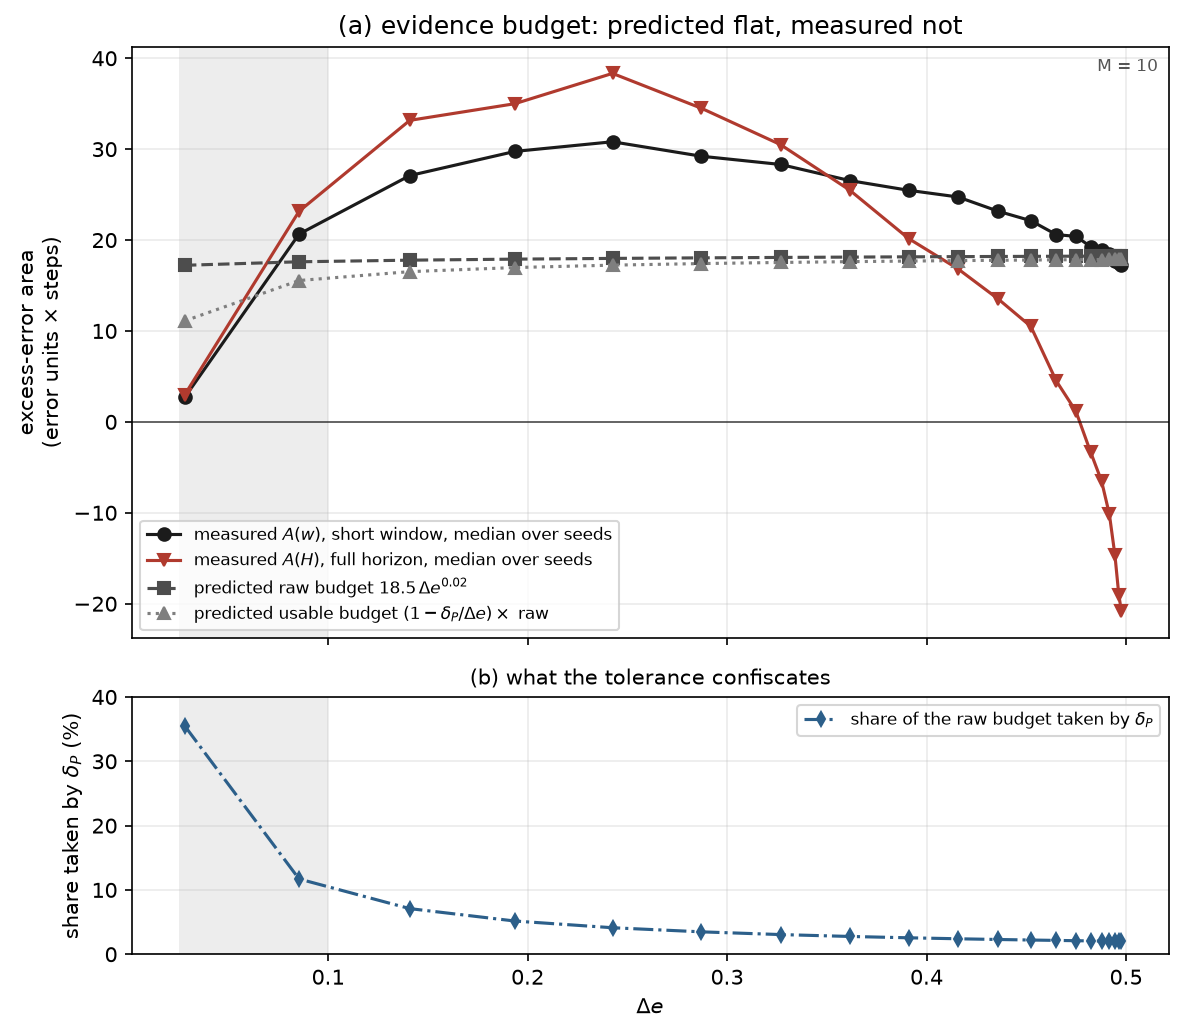
\includegraphics[height=0.66\textheight]{Fig_QC_budget_utilisable_full.png}
    \end{column}\hfill
    \begin{column}{0.46\textwidth}
      \begin{itemize}
        \item The paper's picture: an excess error $\Delta e$ over a window $\tau_{\mathrm{ARF}}$,
              so the area stays almost constant.
        \item Measured over the transition, the area varies by a factor of $1.8$ while the
              drift size varies by $5.8$: \alert{the compensation is real}.
        \item But the paper's rectangle misestimates it by up to $43\%$, and over the whole
              horizon the area turns negative at large drifts: the new task is easier.
      \end{itemize}
    \end{column}
  \end{columns}
  \note{Why doesn't a violent drift leave more evidence than a gentle one? The paper's picture
    is a rectangle: an excess error of height delta e, during a window equal to the repair
    time. Since the repair time shrinks like one over delta e, the area stays almost constant.
    We measured the area directly. Over the transition, it varies by a factor of less than two,
    while the drift size varies by almost six: the compensation is real. But the rectangle
    itself is wrong. It misestimates the area by up to forty-three percent, because the first
    replacement is not the width of the transient. And over the whole horizon, at large drifts,
    the area even becomes negative: after the change the task is easier than before, and the
    error settles below its old level. The evidence exists, it is roughly constant, but the
    paper's derivation of it does not hold.}
\end{frame}

\begin{frame}{Detecting is not winning}
  \begin{center}
    \begin{tabular}{@{}cccc@{}}
      \toprule
      threshold $\lambda$ & alarm fires & detector arrives first & false alarms, no drift \\
      \midrule
      $8$  & $95.3\%$ & $\mathbf{91.0\%}$ & $4.15\%$ \\
      $15$ & $92.9\%$ & $\mathbf{36.3\%}$ & $0.15\%$ \\
      $20$ & $66.2\%$ & $8.1\%$           & $0.00\%$ \\
      $25$ & $38.9\%$ & $2.5\%$           & $0.00\%$ \\
      \bottomrule
    \end{tabular}\\[0.3em]
    {\scriptsize\color{gray} $2\,000$ runs with drift and $2\,000$ without, over $2\,000$ steps}
  \end{center}
  \begin{itemize}
    \item At $\lambda = 15$ the alarm almost always fires, but mostly \emph{after} the repair.
    \item At $\lambda = 8$ the detector wins at an ordinary false-alarm cost: the paper's
          ``no threshold escapes'' does not hold on this bench.
    \item \textcolor{gray}{Not tested: the heteroscedastic streams where the paper places its
          false-alarm tension.}
  \end{itemize}
  \note{One practical consequence. Detecting a drift and winning the race are two different
    things. At threshold fifteen, the alarm fires on ninety-three percent of drifts, which
    looks excellent, but it arrives before the repair in only thirty-six percent of them.
    Most of these alarms come after the forest has already changed. At threshold eight, the
    detector wins ninety-one percent of the races, and it costs about four percent of false
    alarms over two thousand steps where nothing happens, which is an ordinary calibration
    level. So on this bench, one threshold does escape the blind spot, and the paper's claim
    that no threshold escapes has to be restricted. We did not test the financial streams
    with clustered volatility, where the paper places the false-alarm problem.}
\end{frame}

% =====================================================================
\section{Conclusion}
% =====================================================================

\begin{frame}{What changes in the paper}
  \small
  \begin{tabular}{@{}p{0.34\textwidth}p{0.43\textwidth}l@{}}
    \toprule
    The paper & Our result & \\
    \midrule
    races the repair against a constant & race identified, bounded, decided run by run & \textbf{made exact} \\
    independent trees, bias asserted & direction proven, cannot reverse & \textbf{proven} \\
    error back to normal at the first replacement & it comes back later; the rectangle fails & \textbf{corrected} \\
    first replacement as the repair date & earliest date, fires without drift & \textbf{qualified} \\
    transition between $15$ and $25$, unexplained & set by the evidence before the repair & \textbf{explained} \\
    no threshold escapes & $\lambda = 8$ does, on this bench & \textbf{restricted} \\
    \bottomrule
  \end{tabular}
  \vspace{0.6em}
  \begin{center}
    \alert{The phenomenon survives. What changes is its mechanism and its reach.}
  \end{center}
  \note{To sum up what our work changes in the paper. The race, which compared a random time
    with a constant, is made exact: identified, bounded, and decided run by run. The bias of
    the independence assumption was asserted; it is now proven, with its direction. The idea
    that the error is back to normal at the first replacement is corrected. The first
    replacement as a repair date is qualified: it is the earliest date and it fires without
    drift. The transition threshold, which the paper left unexplained, is explained by the
    evidence before the repair. And the claim that no threshold escapes is restricted to the
    settings the paper actually tested. The phenomenon survives all of this. What changes is
    its mechanism, and its reach.}
\end{frame}

\begin{frame}{An open question, and what we did not do}
  \begin{columns}[T,onlytextwidth]
    \begin{column}{0.50\textwidth}
      \begin{exampleblock}{Open: a reference for adaptation}
        Every indicator on the detector's side reads the \emph{error}, which mixes what the
        forest relearned with how hard the new task is. On analytic probes, the forest can
        relearn the changed region and lose a rare one, unseen by the error.
      \end{exampleblock}
    \end{column}\hfill
    \begin{column}{0.46\textwidth}
      \begin{block}{Not done}
        \small
        \begin{itemize}
          \item one forest size, one homoscedastic bench
          \item decision rule fixed during the analysis
          \item the independence bias has a sign, not a size
        \end{itemize}
      \end{block}
    \end{column}
  \end{columns}
  \note{We leave one question open. Every measure available to the detector reads the error,
    and the error mixes two things: what the forest has relearned, and how hard the new task
    is. Using analytic probes, points whose true label we know, we saw that the forest can
    relearn the region that changed while losing a rare region elsewhere, and the error does
    not see that loss. So what would a true reference for adaptation be? We do not have the
    answer. And to be honest about the limits: we studied one forest size on one simple
    bench, our decision rule was fixed during the analysis rather than before it, and we can
    give the sign of the independence bias but not its size.}
\end{frame}

\begin{frame}{Take-away}
  \begin{center}
    \small\alert{The blind spot is a budget of evidence, accumulated before the repair, set
    against a threshold.}
  \end{center}
  \vspace{-0.5em}
  \begin{center}\carte[0.71]{0}\end{center}
  \note{Back to the map. The blind spot is real, and it survives every correction. But it is
    not a race between two clocks. It is the evidence the forest lets through before its first
    repair, set against a fixed threshold. That single quantity explains when the detector
    wins, why the transition sits where it does, and why stronger drifts are missed more
    often. Thank you for your attention; we are happy to take your questions.}
\end{frame}

% =====================================================================
\appendix
\section*{Backup}
% =====================================================================

\begin{frame}{Backup --- Fréchet bounds}
  For integer-valued clocks with marginal CDFs $F_A$ and $F_D$, and \emph{any} coupling,
  \begin{align*}
    P_{\mathrm{miss}} &\ge \max\Big(0,\ \sup_{s} \big[F_A(s)-F_D(s)\big]\Big),\\
    P_{\mathrm{miss}} &\le \min\Big(1,\ \inf_{s} \big[F_A(s) + 1 - F_D(s+1)\big]\Big).
  \end{align*}
  \begin{itemize}
    \item Lower: Fréchet on $\{\tau_{\mathrm{ARF}} \le s < \tau_{\mathrm{det}}\} \subseteq \mathrm{Miss}$.
    \item Upper: $\mathrm{Miss} \subseteq \{\tau_{\mathrm{ARF}} \le s\} \cup \{\tau_{\mathrm{det}} > s+1\}$, then Boole.
    \item Toy case, both clocks uniform on $\{1,2\}$: the bounds $0$ and $0.5$ are both attained.
  \end{itemize}
\end{frame}

\begin{frame}{Backup --- Lindley's closed form and the certificate}
  With $X_t = e_t - \hat p_0 - \delta_P$ and $A(k,j) = \sum_{t=k+1}^{j} (e_t - \hat p_0)$,
  \[
    S_j = \max_{0 \le k \le j} \sum_{t=k+1}^{j} X_t,
    \qquad
    S_{\max}(H) = \max_{0 \le k \le j \le H} \big[A(k,j) - (j-k)\,\delta_P\big].
  \]
  \begin{itemize}
    \item Certificate: the alarm fires by $H$ iff some sub-window carries
          $A(k,j) \ge \lambda + (j-k)\,\delta_P$. The full window alone is only sufficient.
    \item Race identity: the same maximum, taken up to the first replacement, is $S_{\mathrm{pre}}$.
  \end{itemize}
\end{frame}

\begin{frame}{Backup --- Association protocol}
  \begin{itemize}
    \item Every coefficient is computed \textbf{within a drift size} ($100$ seeds), on the $18$
          sizes with $\Delta e \ge 0.10$: pooling measures the drift size, not the link.
    \item Kendall's $\tau_b$: reads on pairs, corrects for ties. Censored durations ranked last,
          licit because the horizon is common to all runs.
    \item Pearson undefined on censored values; Spearman handles their ties implicitly.
    \item Percentile bootstrap over seeds, $2\,000$ resamples; discernible if the interval
          excludes zero. Fixed during the analysis, not before: stated in the report.
    \item Complete cases instead of ranking censored runs last: no coefficient moves by more
          than $0.0403$.
  \end{itemize}
\end{frame}

\begin{frame}{Backup --- The drift-free control}
  \begin{center}
    \begin{tabular}{@{}lr@{}}
      \toprule
      On $2\,000$ runs with no change point & \\
      \midrule
      runs where at least one tree is replaced & $2\,000/2\,000$ \\
      first replacement, median & $95$ steps \\
      distinct trees renewed, median & $9/10$ \\
      forest entirely renewed & $28.7\%$ \\
      \midrule
      first replacement at the weakest drift, median & $118$ steps \\
      \bottomrule
    \end{tabular}
  \end{center}
\end{frame}

\end{document}
"
%
% Tracabilite : chaque chiffre vient du rapport ; controle par
%   verif_chiffres_tex.py ../../05_presentation/soutenance_20min.tex
% Figures : figures_slides.py --latex, figures_soutenance.py,
%   matrice_correlations.py, analyse_QCD.py (budget).
% =====================================================================

\documentclass[aspectratio=169,11pt]{beamer}

\usetheme{Madrid}
% Rouge de CentraleSupelec, pris dans le logo officiel (#B00739) ; logo
% CentraleSupelec / Universite Paris-Saclay sur la page de titre.
\definecolor{csRouge}{HTML}{B00739}
\usecolortheme[named=csRouge]{structure}
\setbeamercolor{alerted text}{fg=csRouge}
\setbeamersize{text margin left=1cm, text margin right=1cm}
\setbeamertemplate{navigation symbols}{}
\usepackage[english,french]{babel}
\usepackage{amsmath,amssymb}
\usepackage{graphicx}
\usepackage{booktabs}
\usepackage{tikz}
% soutenance_schemas.tex
% =====================================================================
% Schemas TikZ de `soutenance_20min.tex` : la carte des idees et le schema
% de l'identite de course.
%
% Fichier separe pour la meme raison que `point_encadrant_schemas.tex` :
% `verif_chiffres_tex.py` ramasserait les coordonnees TikZ comme des mesures.
% AUCUN chiffre de mesure ici ; les schemas sont stylises, sans donnees.
% =====================================================================

\usetikzlibrary{positioning, arrows.meta, calc}

\definecolor{mTheorie}{RGB}{31,58,104}
\definecolor{mDate}{RGB}{138,28,28}
\definecolor{mPreuve}{RGB}{38,92,58}
\definecolor{mEteint}{gray}{0.74}

% ---------------------------------------------------------------------
% \carte[hauteur]{k} : la carte des idees.
%   k = 0 : tout est actif (ouverture et conclusion)
%   k = 1, 2, 3 : seule la partie k est en couleur, le reste est grise
%   hauteur : fraction de \textheight (0.80 par defaut)
% Les fleches en pointille relient les parties ; elles sont commentees a
% l'oral plutot qu'etiquetees, faute de place entre les colonnes.
% ---------------------------------------------------------------------
\newcommand{\carte}[2][0.80]{%
  \colorlet{cUn}{mEteint}\colorlet{cDeux}{mEteint}\colorlet{cTrois}{mEteint}%
  \colorlet{tUn}{mEteint}\colorlet{tDeux}{mEteint}\colorlet{tTrois}{mEteint}%
  \ifnum#2=0 \colorlet{cUn}{mTheorie}\colorlet{cDeux}{mDate}\colorlet{cTrois}{mPreuve}%
    \colorlet{tUn}{black}\colorlet{tDeux}{black}\colorlet{tTrois}{black}\fi
  \ifnum#2=1 \colorlet{cUn}{mTheorie}\colorlet{tUn}{black}\fi
  \ifnum#2=2 \colorlet{cDeux}{mDate}\colorlet{tDeux}{black}\fi
  \ifnum#2=3 \colorlet{cTrois}{mPreuve}\colorlet{tTrois}{black}\fi
  \resizebox{!}{#1\textheight}{%
  \begin{tikzpicture}[
      font=\normalsize, align=center,
      boite/.style={draw, line width=1pt, rounded corners=3pt, inner sep=4pt,
                    text width=4.3cm, minimum height=1.05cm},
      un/.style={boite, draw=cUn, text=tUn},
      deux/.style={boite, draw=cDeux, text=tDeux},
      trois/.style={boite, draw=cTrois, text=tTrois},
      tete/.style={font=\bfseries\normalsize, text width=4.8cm},
      fl/.style={-{Stealth[length=2.4mm]}, line width=0.9pt},
      lien/.style={-{Stealth[length=2.4mm]}, line width=0.9pt, dashed},
    ]
    \node[boite, draw=black, fill=black!4, text width=12cm, minimum height=0.8cm] (P) at (5.6,0.15)
      {\textbf{The paper:} the stronger the drift, the faster the repair, the fewer the alarms};

    \node[tete, text=cUn]    (H1) at (0,-1.05)    {I.\ The race, formally};
    \node[tete, text=cDeux]  (H2) at (5.6,-1.05)  {II.\ The repair date};
    \node[tete, text=cTrois] (H3) at (11.2,-1.05) {III.\ Evidence vs threshold};
    \draw[fl, black!55] (P.south) -- ++(0,-0.25) -| (H1.north);
    \draw[fl, black!55] (P.south) -- (H2.north);
    \draw[fl, black!55] (P.south) -- ++(0,-0.25) -| (H3.north);

    \node[un] (A1) at (0,-2.1)  {The miss is well defined, its probability identified};
    \node[un] (A2) at (0,-3.45) {The blind spot holds whatever the dependence};
    \node[un] (B1) at (0,-4.8)  {Independent trees overstate the speed of repair};

    \node[deux] (C1) at (5.6,-2.1)  {The first replacement is the earliest date};
    \node[deux] (E1) at (5.6,-3.45) {It fires as fast when nothing changes};
    \node[deux] (D1) at (5.6,-4.8)  {When it fires, half the evidence is there};
    \node[deux] (D2) at (5.6,-6.15) {Indicators form two groups, weakly linked};

    \node[trois] (C2) at (11.2,-2.1)  {The alarm is a function of the error path};
    \node[trois] (K)  at (11.2,-3.45) {Detector first \emph{iff} it reaches $\lambda$ before the repair};
    \node[trois] (S)  at (11.2,-4.8)  {That evidence sets the transition and the paradox};
    \node[trois] (T)  at (11.2,-6.15) {Detecting is not winning};

    \node[boite, draw=black!55, text=black!80, dashed, text width=7cm, minimum height=0.8cm] (O) at (5.6,-7.45)
      {\textbf{Open:} a reference for adaptation itself};

    \draw[fl, cUn]    (A1) -- (A2);
    \draw[fl, cDeux]  (C1) -- (E1);
    \draw[fl, cDeux]  (E1) -- (D1);
    \draw[fl, cDeux]  (D1) -- (D2);
    \draw[fl, cTrois] (C2) -- (K);
    \draw[fl, cTrois] (K) -- (S);
    \draw[fl, cTrois] (S) -- (T);
    \draw[lien, black!55] (B1.east) -- (D1.west);
    \draw[lien, black!55] (D1.east) -- (S.west);
    \draw[lien, black!55] (D2.south) -- (O.north);
  \end{tikzpicture}}%
}

% ---------------------------------------------------------------------
% \schemaidentite : la pile S_t, le premier remplacement, deux seuils.
% Stylise, sans donnees.
% ---------------------------------------------------------------------
\newcommand{\schemaidentite}{%
  \begin{tikzpicture}[x=1cm, y=1cm, font=\small]
    \draw[-{Stealth}, line width=0.7pt] (0,0) -- (7.2,0);
    \node[below left] at (7.2,-0.05) {time};
    \draw[-{Stealth}, line width=0.7pt] (0,0) -- (0,3.7);
    \node[rotate=90, above] at (-0.05,1.85) {detector statistic $S_t$};
    \draw[line width=1.4pt, mTheorie]
      (0,0) .. controls (0.8,0.6) and (1.6,1.9) .. (2.4,2.25)
            .. controls (3.0,2.5) and (3.4,2.55) .. (3.9,2.4)
            .. controls (4.8,2.0) and (5.8,1.0) .. (7.0,0.3);
    \draw[dashed, mDate, line width=1pt] (2.8,0) -- (2.8,3.4);
    \node[above, text=mDate] at (2.8,3.4) {first replacement};
    \fill[mTheorie] (2.8,2.38) circle (2.3pt);
    \node[above left, text=mTheorie] at (2.75,2.4) {$S_{\mathrm{pre}}$};
    \draw[mPreuve, line width=1pt] (0,1.5) -- (7.0,1.5);
    \node[above left, text=mPreuve] at (7.0,1.5) {low $\lambda$: reached before};
    \draw[mDate, line width=1pt, dash dot] (0,3.0) -- (7.0,3.0);
    \node[above left, text=mDate] at (7.0,3.0) {high $\lambda$: not reached};
  \end{tikzpicture}%
}

\titlegraphic{
\includegraphics[height=1.7cm]{Logo_CS_Paris_Saclay.png}}
\ifdefined\NOTESSEULES\setbeameroption{show only notes}\fi
\graphicspath{{../04_experimentations/resultats_R2/resultats/figures/slides_latex/}{../04_experimentations/resultats_R2/resultats/figures/}}

\setbeamerfont{author}{size=\small}
\setbeamerfont{institute}{size=\scriptsize}

\title[The Blind Spot Paradox]{The Blind Spot Paradox}
\subtitle{Formalizing the race and measuring the adaptation}
\author[Boyer, Gouillou, Fonvielle, Petit-Tichanné]{Alexandre Boyer \and Melaine Gouillou \and Salomé Fonvielle \and Ulysse Petit-Tichanné}
\institute[CS]{Research Track, Topic 39, CentraleSupélec. Supervisor: Raphaël Minato}
\date{16 September 2026}

\begin{document}

\maketitle
\note{Bonjour à tous. Notre sujet est le paradoxe du point aveugle : un modèle qui se
  répare lui-même peut détruire la preuve même dont son propre moniteur a besoin. Dans
  les vingt prochaines minutes, nous présenterons ce que nous avons formalisé, ce que
  nous avons mesuré, et la lecture unique qui relie les deux.}

% =====================================================================
\section{The problem}
% =====================================================================

\begin{frame}{Concept drift: the rule changes, the data does not}
  \vspace{-0.6em}
  \[
    \underbrace{P(X)}_{\text{the data}}\ \text{unchanged}
    \qquad\qquad
    \underbrace{P(Y \mid X)}_{\text{the rule}}\ \text{changes}
  \]
  \vspace{-0.9em}
  \begin{center}
    
\includegraphics[height=0.50\textheight]{Fig_slide_drift.png}
  \end{center}
  \begin{center}
    A model trained before the change is now \alert{wrong on the shaded band}.
  \end{center}
  \note{Un classifieur apprend une règle à partir de données. Dans un flux, cette règle peut
    changer alors que les entrées gardent exactement la même distribution. C'est le concept
    drift : P de X ne bouge pas, P de Y sachant X bouge. C'est la situation normale d'un
    signal financier, où les mêmes entrées cessent de vouloir dire la même chose. Sur le banc
    que nous utilisons, des points du plan sont séparés par une droite. Au changement, la
    droite se déplace. Chaque point de la bande grisée change d'étiquette, si bien qu'un
    modèle entraîné avant le changement continue de prédire avec assurance, et se trompe
    désormais sur cette bande. La largeur de la bande est la taille du drift, notée delta e.}
\end{frame}

\begin{frame}{Two defences that run at the same time}
  \begin{columns}[T,onlytextwidth]
    \begin{column}{0.49\textwidth}
      \centering
      \textbf{The model repairs itself}\\[0.3em]
      
\includegraphics[width=\textwidth]{Fig_slide_foret.png}\\[0.2em]
      \small Adaptive Random Forest: ten trees, each replaced when its own error rises.
    \end{column}\hfill
    \begin{column}{0.49\textwidth}
      \centering
      \textbf{A monitor raises the alarm}\\[0.3em]
      
\includegraphics[width=\textwidth]{Fig_slide_watchdog.png}\\[0.2em]
      \small Each error adds to a statistic $S_t$; the alarm fires when it crosses $\lambda$.
    \end{column}
  \end{columns}
  \note{Deux défenses sont déployées ensemble. La première vit à l'intérieur du modèle. La
    forêt aléatoire adaptative est faite de dix arbres de décision qui votent. Chaque arbre
    surveille sa propre erreur avec un petit détecteur, et quand cette erreur monte, l'arbre
    est remplacé par un neuf. La forêt se répare localement, sans demander à personne. La
    seconde défense est à l'extérieur. Un détecteur cumulatif, un test de Page-Hinkley,
    surveille l'erreur de toute la forêt. Chaque erreur pousse une statistique vers le haut
    de presque un, chaque bonne réponse la tire un peu vers le bas, jamais sous zéro. Quand
    la statistique franchit un seuil lambda, l'alarme part, et cette alarme est la seule
    chose qu'un opérateur humain voit.}
\end{frame}

\begin{frame}{The paradox, and what the reviewers asked}
  \begin{columns}[c,onlytextwidth]
    \begin{column}{0.50\textwidth}
      \centering
      
\includegraphics[width=\textwidth]{Fig_slide_mecanisme.png}\\
      {\scriptsize\color{gray} schematic}
    \end{column}\hfill
    \begin{column}{0.46\textwidth}
      \begin{block}{The paper's claim}
        The stronger the drift, the faster the repair, and the \alert{fewer} alarms.
      \end{block}
      \begin{alertblock}{Two corrections requested}
        \begin{enumerate}
          \item It races a random repair time against a \emph{constant}, and assumes the
                trees independent.
          \item It dates the repair at the \emph{first} tree replaced, without showing
                that this date means anything.
        \end{enumerate}
      \end{alertblock}
    \end{column}
  \end{columns}
  \note{Quand les deux défenses tournent ensemble, il se passe quelque chose d'inattendu. Le
    drift commence, les erreurs s'accumulent dans le détecteur, mais la forêt remplace des
    arbres, les erreurs s'arrêtent, et le tas se vide avant d'atteindre le seuil. L'article
    que nous étudions appelle cela le paradoxe du point aveugle : plus le drift est fort,
    plus la forêt se répare vite, et moins l'opérateur reçoit d'alarmes. L'article a été
    relu, et deux corrections ont été demandées. D'abord, il compare un temps de réparation
    aléatoire à un temps de détection constant, et il suppose les dix arbres indépendants
    sans le prouver. Ensuite, il date la réparation au moment où le premier arbre est
    remplacé, sans montrer que ce moment a quoi que ce soit à voir avec la disparition de
    l'erreur. C'est de ces deux corrections que part notre travail.}
\end{frame}

\begin{frame}{Our reading, in one map}
  \begin{center}
    \small\alert{The blind spot is not a race between two clocks,
    but a budget of evidence set against a threshold.}
  \end{center}
  \vspace{-0.5em}
  \begin{center}
    \carte[0.71]{0}
  \end{center}
  \note{Voici tout l'exposé sur une seule carte. En haut, l'affirmation de l'article. La
    première colonne formalise la course : nous définissons proprement le point aveugle,
    nous calculons sa probabilité, et nous montrons que supposer les arbres indépendants
    rend l'article optimiste sur la réparation. La deuxième colonne demande ce que la date
    de réparation mesure réellement : c'est la date la plus précoce possible, elle se
    déclenche même quand rien ne change, et quand elle se déclenche l'essentiel de la preuve
    est déjà là. La troisième colonne relie les deux : le détecteur gagne exactement quand sa
    preuve atteint le seuil avant la réparation, et cette preuve explique à la fois la
    transition et le paradoxe. Les flèches en pointillés sont les liens entre colonnes, et
    la boîte du bas est la question que nous laissons ouverte. Notre lecture en une phrase :
    le point aveugle n'est pas une course entre deux horloges, c'est un budget de preuve
    face à un seuil.}
\end{frame}

% =====================================================================
\section{I. The race}
% =====================================================================

\begin{frame}{Part I --- The race, formally}
  \begin{center}\carte{1}\end{center}
  \note{Commençons par la théorie : comment énoncer la course sans tricher.}
\end{frame}

\begin{frame}{The race is well posed, and its probability identified}
  \begin{columns}[T,onlytextwidth]
    \begin{column}{0.46\textwidth}
      \begin{block}{One definition, no ad hoc rule}
        \[
          \mathrm{Miss} := \{\tau_{\mathrm{ARF}} < \tau_{\mathrm{det}}\}
        \]
        \vspace{-0.6em}
        {\small strict inequality; the alarm may never come}
        \begin{itemize}
          \item a tie goes to the detector
          \item a silent repair, with no alarm ever, \alert{is} a miss
          \item if neither acts, it is not
        \end{itemize}
      \end{block}
    \end{column}\hfill
    \begin{column}{0.50\textwidth}
      \begin{exampleblock}{What the campaign allows}
        The forest always replaces a tree within the horizon, so no run is left
        undecided: $P_{\mathrm{miss}}$ is \textbf{identified}.\\[0.3em]
        \centering
        {\small all $20$ drift sizes pooled:}\\[0.1em]
        \begin{tabular}{@{}lccc@{}}
          $\lambda$ & $8$ & $25$ & $50$ \\
          $P_{\mathrm{miss}}$ & $0.0905$ & $0.9715$ & $1.0000$
        \end{tabular}
      \end{exampleblock}
      \begin{alertblock}{Without any dependence assumption}
        From the marginal laws alone, the blind spot at the weakest drift
        ($\Delta e = 0.028$, observed $1.00$) is at least $0.91$ at $\lambda = 8$.
      \end{alertblock}
    \end{column}
  \end{columns}
  \vspace{0.3em}
  {\scriptsize\color{gray} $\tau_{\mathrm{ARF}}$: first tree replaced \quad
   $\tau_{\mathrm{det}}$: first alarm \quad $\Delta e$: drift size, the jump in error}
  \note{L'article dit qu'il y a point aveugle quand la forêt se répare avant l'alarme, mais
    il écarte discrètement les runs où l'alarme ne vient jamais. Ce sont exactement les runs
    où le détecteur échoue le plus. Nous définissons donc l'événement sur la course
    complète, avec une seule définition et aucune règle supplémentaire. Une égalité compte
    pour le détecteur, parce que l'opérateur est prévenu au bon moment. Une réparation
    silencieuse, où l'alarme ne vient jamais, est un raté, et même le plus pur. Un run où
    aucun des deux mécanismes n'agit n'est pas un raté, parce qu'il n'y avait rien à
    effacer. Vient ensuite le problème de l'horizon fini : certains runs pourraient rester
    indécis. Sur notre campagne ils ne le sont pas, parce que la forêt agit toujours avant
    l'horizon, donc la probabilité de raté est identifiée exactement : neuf pour cent au
    seuil huit, quatre-vingt-dix-sept à vingt-cinq, cent à cinquante. Et avec les bornes de
    Fréchet, qui n'utilisent que les deux lois marginales et ne supposent rien sur le
    couplage des horloges, le point aveugle au drift le plus faible est déjà forcé au-dessus
    de quatre-vingt-dix pour cent.}
\end{frame}

\begin{frame}{Trees share a stream: the paper is optimistic}
  \begin{enumerate}
    \item \textbf{Given the stream}, what separates two trees is their own random draws:
          the trees are independent \emph{conditionally}.
    \item \textbf{Hence the covariance of two trees is a variance}, never negative: sharing
          a stream can only make them fail together --- the forest is \emph{slower} than
          the independence formula says.
    \item \textbf{More precisely}, averaging over streams, convexity gives the bound:
          \[
            P(\tau_{\mathrm{ARF}} \le s) \;\le\; 1 - \big(1 - F(s)\big)^M
          \]
    \item \textbf{Conclusion}: \alert{the independence formula overstates the speed of
          the repair}, hence the blind spot; the paper's critical ensemble size becomes a
          conservative ceiling, and its verdict does not change.
  \end{enumerate}
  \note{Le second raccourci est l'indépendance. Les dix arbres apprennent sur le même flux,
    ils ne peuvent donc pas être indépendants. Mais la question est : à quel niveau. Une
    fois le flux fixé, ce qui distingue un arbre d'un autre n'est plus que son aléa propre,
    les poids aléatoires du bagging en ligne. À ce niveau, sachant le flux, les arbres sont
    indépendants. C'est une propriété de l'algorithme, et tout le reste en découle. D'abord
    le sens : le seul canal entre deux arbres est le flux qu'ils partagent, et un flux
    partagé ne peut que les faire échouer ensemble, puisque leur covariance se réduit à une
    variance. La vraie forêt se répare donc plus lentement que ne le dit la formule
    d'indépendance. Ensuite la taille : en moyennant sur les flux, l'inégalité de Jensen
    donne une majoration, la probabilité que la forêt se soit déjà réparée est au plus ce
    que la formule d'indépendance prédit. L'article fait donc paraître la forêt plus rapide
    qu'elle n'est, et surestime le point aveugle. Sa taille critique d'ensemble n'est pas
    fausse, elle devient un plafond conservateur, et le verdict de l'article lui-même ne
    change pas.}
\end{frame}

% =====================================================================
\section{II. The repair date}
% =====================================================================

\begin{frame}{Part II --- What the repair date measures}
  \begin{center}\carte{2}\end{center}
  \note{Passons à la seconde correction : la date que l'article utilise pour la réparation.}
\end{frame}

\begin{frame}{How we measured}
  \begin{columns}[T,onlytextwidth]
    \begin{column}{0.48\textwidth}
      \begin{block}{The campaign}
        \begin{itemize}
          \item the paper's bench, rerun: $20$ drift sizes $\times$ $100$ seeds,
                $2\,000$ steps after the change
          \item $2\,000$ more runs with no change at all
          \item only the error and the replacement events are recorded; every threshold is
                replayed offline
        \end{itemize}
      \end{block}
    \end{column}\hfill
    \begin{column}{0.48\textwidth}
      \begin{block}{Reading an association}
        \begin{itemize}
          \item always \alert{within one drift size}: pooling measures the drift size, not
                the link
          \item Kendall's rank correlation, with bootstrap intervals over the seeds
          \item steps added after seeing the data are flagged as exploratory
        \end{itemize}
      \end{block}
    \end{column}
  \end{columns}
  \note{Un mot sur la façon dont nous avons mesuré, sans les détails d'implémentation. Nous
    avons rejoué le banc de l'article sur vingt tailles de drift, avec cent graines chacune,
    et nous observons deux mille pas après le changement. Nous avons ajouté deux mille runs
    où rien ne change du tout, comme témoin. La simulation n'enregistre que deux choses :
    l'erreur à chaque pas et les instants où des arbres sont remplacés. Tout le reste, y
    compris le détecteur à n'importe quel seuil, est recalculé hors ligne, si bien qu'une
    campagne en remplace plusieurs. Quand nous corrélons deux grandeurs, nous le faisons
    toujours à taille de drift fixée. La taille du drift déplace tous les indicateurs à la
    fois, donc une corrélation mélangeant les tailles mesure surtout la taille elle-même.
    Nous utilisons la corrélation de rang de Kendall avec des intervalles bootstrap, et nous
    signalons les étapes ajoutées après avoir regardé les données.}
\end{frame}

\begin{frame}{The first replacement is the earliest possible date}
  \begin{center}
    
\includegraphics[width=0.90\textwidth]{Fig_slide_deux_horloges.png}
  \end{center}
  \vspace{-0.3em}
  \begin{itemize}
    \item On every run, the first replacement comes before any other quota of renewed
          trees. Three quarters of the forest are renewed \textbf{$6.0$ to $14.3$ times later}.
    \item \alert{With no drift at all}, the first replacement comes after $95$ steps in
          median, against $118$ on the weakest drift.
    \item On weak drifts it comes \emph{later}: $346$ steps at $\Delta e = 0.085$. With no drift
          but the same error level, it also waits $268$: the error level delays it, not the change.
  \end{itemize}
  \note{L'article date la réparation au premier arbre remplacé. Par construction, c'est la
    plus précoce de toutes les dates possibles : le moment où trois arbres, ou la moitié, ou
    les trois quarts de la forêt sont remplacés vient toujours après, sur chaque run. La
    seule question est : combien de temps après. Sur ce drift moyen, le premier arbre tombe
    après quatre-vingt-six observations, et les trois quarts de la forêt après plus de douze
    cents. Sur la grille, les trois quarts de la forêt sont renouvelés six à quatorze fois
    plus tard que le premier arbre. Et il y a un fait plus inquiétant. Sur les deux mille
    runs sans aucun changement, la forêt remplace quand même son premier arbre, après
    quatre-vingt-quinze pas en médiane. Sur le drift réel le plus faible, il lui en faut cent
    dix-huit. Donc à faible drift, cette date ne distingue pas un vrai changement du bruit.
    Pire, sur un drift un peu plus fort elle vient plus tard, après trois cent quarante-six
    pas. Nous avons vérifié pourquoi avec un second témoin sans drift, où l'on élève seulement
    le niveau d'erreur en retournant des étiquettes. Au même niveau d'erreur, le premier
    remplacement attend aussi environ deux cent soixante-dix pas. Le détecteur interne de
    chaque arbre coupe moins souvent quand l'erreur est plus bruitée, donc sur les drifts
    faibles cette date mesure le niveau d'erreur, pas le changement.}
\end{frame}

\begin{frame}{When the first tree goes, most of the evidence is already there}
  \begin{columns}[T,onlytextwidth]
    \begin{column}{0.36\textwidth}
      \begin{block}{Evidence at the first replacement}
        \centering
        {\Large $49\%$ to $76\%$}\\[0.2em]
        \small of the detector's final peak, on the $18$ drift sizes studied
      \end{block}
    \end{column}\hfill
    \begin{column}{0.60\textwidth}
      \begin{block}{Does the date track anything, within a drift size?}
        \small
        \begin{tabular}{@{}lcc@{}}
          \toprule
          compared with & median link & sizes \\
          \midrule
          detector peak & $0.21$ & $15/18$ \\
          excess error, whole horizon & none & $0/18$ \\
          excess error, transition only & $0.23$ & $13/18$ \\
          \bottomrule
        \end{tabular}
      \end{block}
    \end{column}
  \end{columns}
  \vspace{0.8em}
  \begin{center}
    \small The null over the whole horizon is mostly noise: \alert{half} of that area's
    variance comes from the estimated baseline, multiplied by the horizon.
  \end{center}
  \note{Le premier remplacement est-il au moins la fin du transitoire ? Non. Quand le premier
    arbre est remplacé, le détecteur détient déjà entre la moitié et les trois quarts de
    toute la preuve qu'il accumulera jamais. Le remplacement est au milieu de l'histoire, pas
    à sa fin. Nous avons ensuite demandé si cette date suit quelque chose, toujours à taille
    de drift fixée. Avec le pic du détecteur, il y a un lien faible mais réel, visible sur
    quinze tailles de drift sur dix-huit. Avec l'erreur excédentaire sur tout l'horizon, il
    n'y a aucun lien. Mais nous avons compris pourquoi : cette aire additionne deux mille
    pas, donc toute erreur sur le socle est multipliée par deux mille, et la moitié de sa
    variance n'est que ce bruit. Si l'on ne garde que la transition, le lien revient, faible
    mais réel, sur treize tailles sur dix-huit. Cette dernière étape est exploratoire.}
\end{frame}

\begin{frame}{Unexpected: pooling manufactures agreement}
  \begin{center}
    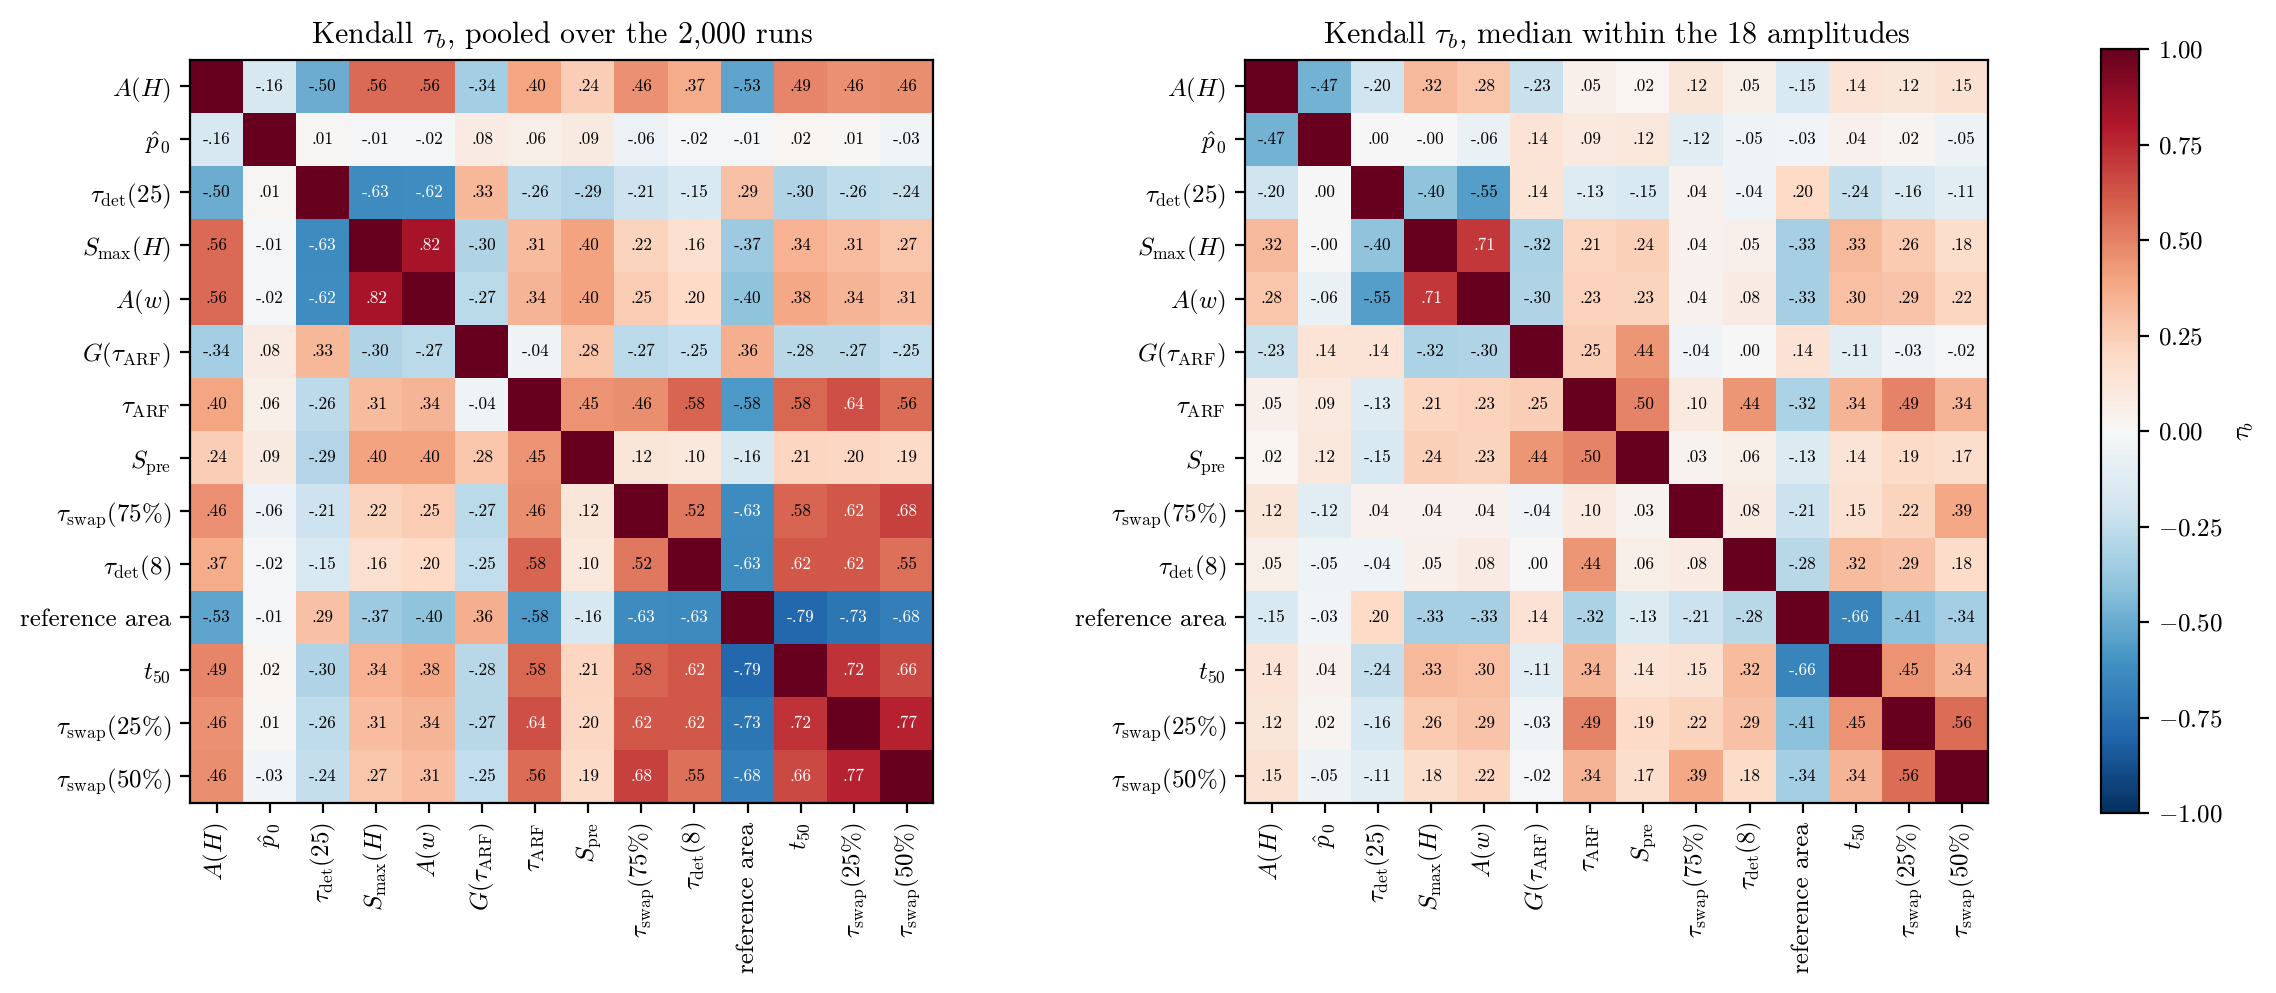
\includegraphics[width=0.86\textwidth]{Fig_QD_matrice_correlations_full.png}
  \end{center}
  \vspace{-0.5em}
  \small
  \begin{columns}[T,onlytextwidth]
    \begin{column}{0.32\textwidth}
      \textbf{Left, pooled:} almost everything agrees, because the drift size moves every
      indicator.
    \end{column}\hfill
    \begin{column}{0.32\textwidth}
      \textbf{Right, within a size:} two groups remain, \emph{evidence} ($0.71$) and
      \emph{repair}, weakly joined.
    \end{column}\hfill
    \begin{column}{0.32\textwidth}
      Best date against the analytic reference: \alert{3 trees replaced}, $0.45$, ahead of
      the first tree, $0.34$.
    \end{column}
  \end{columns}
  \note{Pour voir tous les indicateurs d'un coup, nous en avons croisé quatorze. Le panneau
    de gauche mélange tous les runs : presque tout est fortement corrélé avec tout. C'est une
    illusion, le paradoxe de Simpson : la taille du drift déplace chaque indicateur, donc le
    mélange fabrique de l'accord. Le panneau de droite calcule les mêmes corrélations à
    l'intérieur de chaque taille de drift. L'essentiel de l'accord disparaît, et deux groupes
    subsistent. Un groupe mesure la preuve et les dégâts : le pic du détecteur et l'erreur
    excédentaire sur la transition s'accordent fortement. L'autre groupe mesure la
    réparation. Entre les deux groupes, les liens restent faibles. Nous avons aussi comparé
    les dates de remplacement à une référence analytique, la précision de la forêt sur la
    région dont l'étiquette a changé. La date à laquelle trois arbres sont remplacés la suit
    mieux que le premier arbre. Cette matrice est exploratoire.}
\end{frame}

% =====================================================================
\section{III. Evidence vs threshold}
% =====================================================================

\begin{frame}{Part III --- Evidence against the threshold}
  \begin{center}\carte{3}\end{center}
  \note{La troisième partie relie les deux premières.}
\end{frame}

\begin{frame}{The race is decided before the repair}
  \begin{columns}[c,onlytextwidth]
    \begin{column}{0.52\textwidth}
      \centering
      \resizebox{\linewidth}{!}{\schemaidentite}\\
      {\scriptsize\color{gray} schematic}
    \end{column}\hfill
    \begin{column}{0.44\textwidth}
      A time counts observations; $\lambda$ counts \emph{excess errors}. Comparing them
      needs a rate that does not exist.
      \begin{block}{Race identity, on every run}
        \vspace{-0.4em}
        \[
          \tau_{\mathrm{det}} < \tau_{\mathrm{ARF}}
          \iff S_{\mathrm{pre}} \ge \lambda
        \]
        \vspace{-0.9em}
        \[
          S_{\mathrm{pre}} = \max_{t < \tau_{\mathrm{ARF}}} S_t
        \]
      \end{block}
      \vspace{-0.3em}
      {\scriptsize\color{gray} $S_{\mathrm{pre}}$: the highest the detector's evidence gets
       before the forest repairs itself\par}
      \vspace{0.3em}
      \small No rate, no averaging, no assumption on the trees. Checked on $2\,000$ runs out
      of $2\,000$ at three thresholds.
    \end{column}
  \end{columns}
  \note{Voici l'étape clé. Un temps de réparation compte des observations. Un seuil compte
    des erreurs excédentaires. Ils ne sont pas dans la même unité, et l'article fait le pont
    avec un taux moyen d'erreurs par pas. Ce taux n'existe pas : il chute à mesure que la
    forêt se répare, et le détecteur oublie sa preuve chaque fois qu'il touche zéro.
    L'énoncé exact est bien plus simple. Regardez la statistique du détecteur jusqu'au
    premier remplacement, et prenez son point le plus haut : nous l'appelons S pré. Le
    détecteur arrive premier si et seulement si S pré atteint le seuil. Avec un seuil bas, il
    est atteint avant la réparation ; avec un seuil haut, il ne l'est pas. C'est exact sur
    chaque run, ça ne demande ni taux, ni moyenne, ni hypothèse sur les arbres, et nous
    l'avons vérifié sur les deux mille runs.}
\end{frame}

\begin{frame}{The evidence before the repair sets the transition}
  \begin{columns}[c,onlytextwidth]
    \begin{column}{0.60\textwidth}
      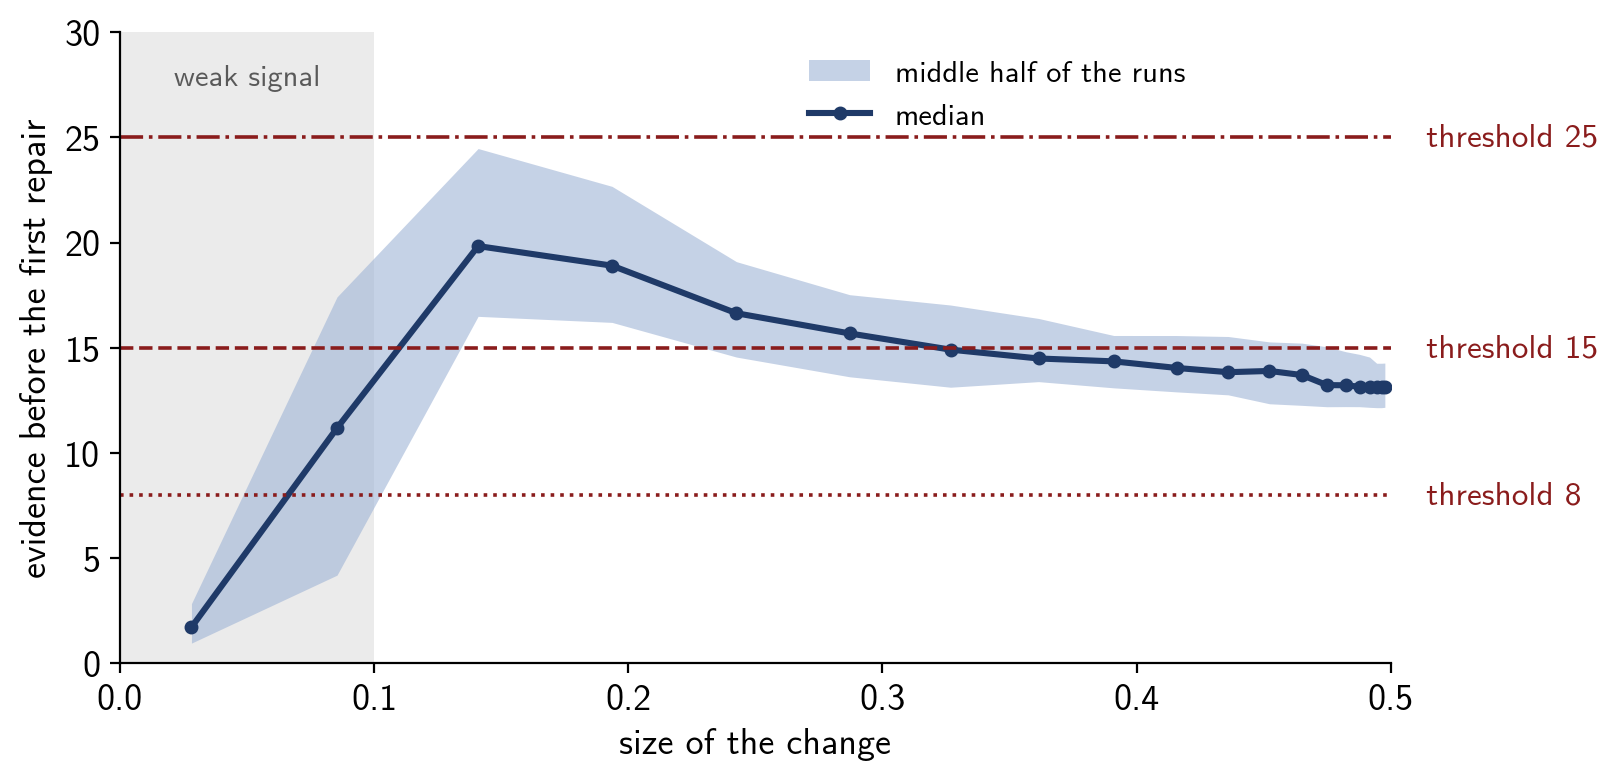
\includegraphics[width=\textwidth]{Fig_slide_spre.png}
    \end{column}\hfill
    \begin{column}{0.37\textwidth}
      \begin{itemize}
        \item Above the weak-signal zone, the median lies between \textbf{$13.1$ and $19.8$}:
              the transition the paper sees between $15$ and $25$, \alert{and leaves
              unexplained}.
        \item It \textbf{decreases} as the drift grows: at $\lambda = 15$ the detector wins
              $81\%$, then only $18\%$. That is the paradox.
      \end{itemize}
    \end{column}
  \end{columns}
  \note{Nous avons donc mesuré S pré sur chaque run. La ligne sombre est la médiane par
    taille de drift, la bande contient la moitié centrale des runs, et les lignes rouges sont
    des seuils. Au-dessus de la zone de signal faible, la médiane se situe entre treize et
    vingt. Un seuil sous ce niveau est atteint avant la réparation dans la plupart des runs ;
    un seuil au-dessus l'est rarement. C'est exactement la transition que l'article observe
    entre quinze et vingt-cinq, et qu'il laisse aux travaux futurs. Regardez maintenant la
    forme. Après les drifts moyens, S pré décroît quand le drift se renforce, parce que le
    premier remplacement vient plus tôt. À seuil fixé à quinze, le détecteur gagne
    quatre-vingt-un pour cent des courses sur les drifts moyens, et seulement dix-huit pour
    cent sur les plus forts. Le paradoxe, c'est cette preuve décroissante, lue face à un
    seuil fixe. Tout à gauche, le drift est trop faible pour accumuler quoi que ce soit :
    c'est un autre régime.}
\end{frame}

\begin{frame}{Stronger drifts leave no more evidence}
  \begin{columns}[c,onlytextwidth]
    \begin{column}{0.48\textwidth}
      \centering
      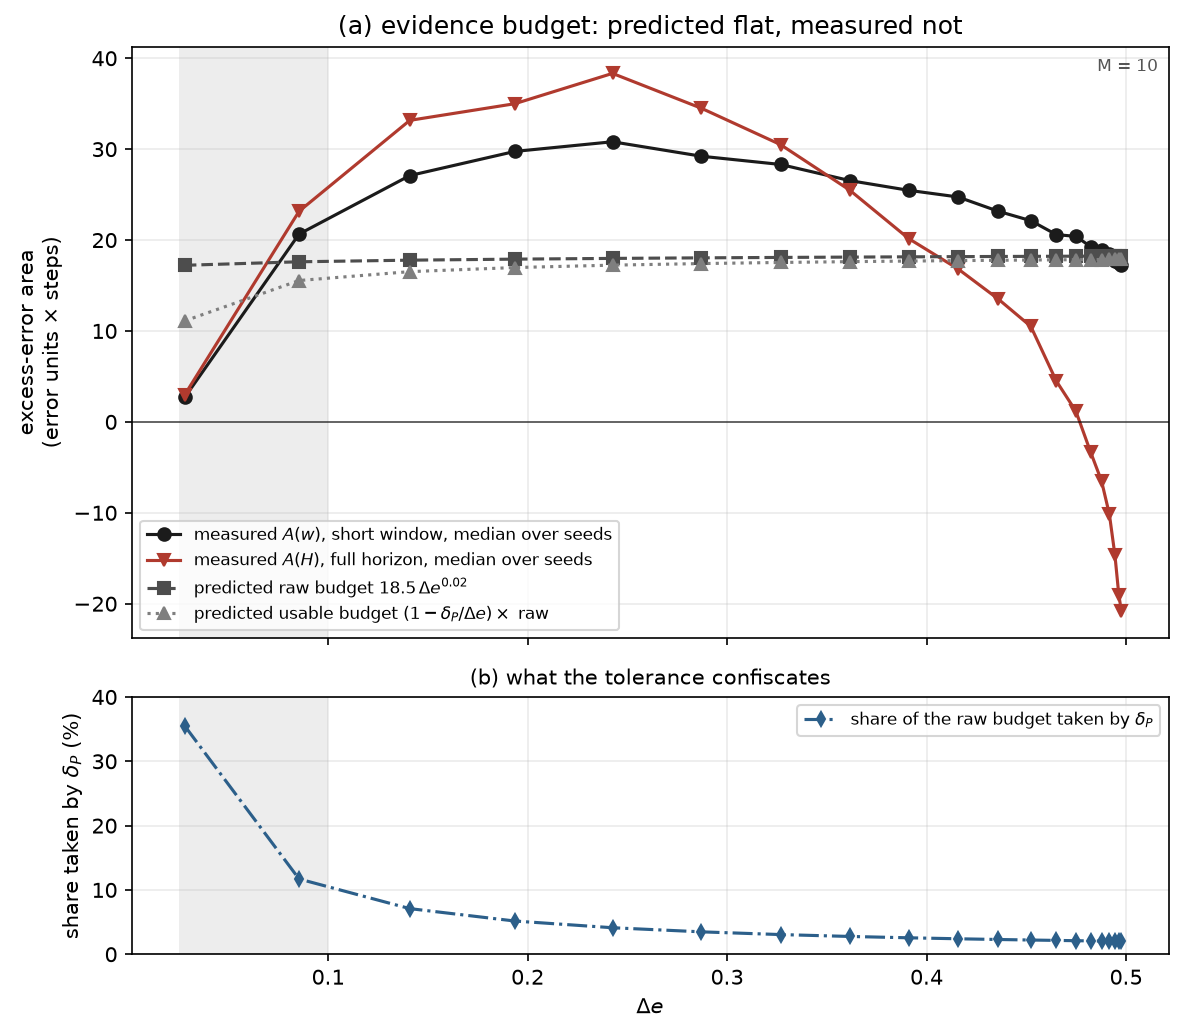
\includegraphics[height=0.66\textheight]{Fig_QC_budget_utilisable_full.png}
    \end{column}\hfill
    \begin{column}{0.46\textwidth}
      \begin{itemize}
        \item The paper's picture: an excess error $\Delta e$ over a window $\tau_{\mathrm{ARF}}$,
              so the area stays almost constant.
        \item Measured over the transition, the area varies by a factor of $1.8$ while the
              drift size varies by $5.8$: \alert{the compensation is real}.
        \item But the paper's rectangle misestimates it by up to $43\%$, and over the whole
              horizon the area turns negative at large drifts: the new task is easier.
      \end{itemize}
    \end{column}
  \end{columns}
  \note{Pourquoi un drift violent ne laisse-t-il pas plus de preuve qu'un drift doux ?
    L'image de l'article est un rectangle : une erreur excédentaire de hauteur delta e,
    pendant une fenêtre égale au temps de réparation. Comme le temps de réparation décroît
    comme un sur delta e, l'aire reste presque constante. Nous avons mesuré l'aire
    directement. Sur la transition, elle varie d'un facteur inférieur à deux, alors que la
    taille du drift varie de presque six : la compensation est réelle. Mais le rectangle
    lui-même est faux. Il se trompe sur l'aire jusqu'à quarante-trois pour cent, parce que le
    premier remplacement n'est pas la largeur du transitoire. Et sur tout l'horizon, aux
    grands drifts, l'aire devient même négative : après le changement, la tâche est plus
    facile qu'avant, et l'erreur se stabilise sous son ancien niveau. La preuve existe, elle
    est à peu près constante, mais la dérivation qu'en fait l'article ne tient pas.}
\end{frame}

\begin{frame}{Detecting is not winning}
  \begin{center}
    \begin{tabular}{@{}cccc@{}}
      \toprule
      threshold $\lambda$ & alarm fires & detector arrives first & false alarms, no drift \\
      \midrule
      $8$  & $95.3\%$ & $\mathbf{91.0\%}$ & $4.15\%$ \\
      $15$ & $92.9\%$ & $\mathbf{36.3\%}$ & $0.15\%$ \\
      $20$ & $66.2\%$ & $8.1\%$           & $0.00\%$ \\
      $25$ & $38.9\%$ & $2.5\%$           & $0.00\%$ \\
      \bottomrule
    \end{tabular}\\[0.3em]
    {\scriptsize\color{gray} $2\,000$ runs with drift and $2\,000$ without, over $2\,000$ steps}
  \end{center}
  \begin{itemize}
    \item At $\lambda = 15$ the alarm almost always fires, but mostly \emph{after} the repair.
    \item At $\lambda = 8$ the detector wins $91\%$ of races for $4.15\%$ of drift-free runs
          with a false alarm: the paper's ``no threshold escapes'' does not hold on this bench.
    \item \textcolor{gray}{Not tested: the heteroscedastic streams where the paper places its
          false-alarm tension.}
  \end{itemize}
  \note{Une conséquence pratique. Détecter un drift et gagner la course sont deux choses
    différentes. Au seuil quinze, l'alarme part sur quatre-vingt-treize pour cent des
    drifts, ce qui paraît excellent, mais elle arrive avant la réparation dans seulement
    trente-six pour cent d'entre eux. La plupart de ces alarmes viennent après que la forêt a
    déjà changé. Au seuil huit, le détecteur gagne quatre-vingt-onze pour cent des courses,
    et environ quatre pour cent des runs où rien ne se passe lèvent une fausse alarme en deux
    mille pas. Au seuil douze, il gagne encore soixante-dix-neuf pour cent des courses, pour
    un demi pour cent de fausses alarmes. Donc sur ce banc, les seuils bas échappent bel et
    bien au point aveugle, et l'affirmation de l'article qu'aucun seuil n'y échappe doit
    être restreinte. Nous n'avons pas testé les flux financiers à volatilité groupée, où
    l'article situe le problème des fausses alarmes.}
\end{frame}

% =====================================================================
\section{Conclusion}
% =====================================================================

\begin{frame}{What changes in the paper}
  \small
  \begin{tabular}{@{}p{0.34\textwidth}p{0.43\textwidth}l@{}}
    \toprule
    The paper & Our result & \\
    \midrule
    races the repair against a constant & race identified, bounded, decided run by run & \textbf{made exact} \\
    independent trees, bias asserted & direction proven, cannot reverse & \textbf{proven} \\
    error back to normal at the first replacement & it comes back later; the rectangle fails & \textbf{corrected} \\
    first replacement as the repair date & earliest date, fires without drift & \textbf{qualified} \\
    transition between $15$ and $25$, unexplained & set by the evidence before the repair & \textbf{explained} \\
    no threshold escapes & $\lambda = 8$ and $12$ do, on this bench & \textbf{restricted} \\
    \bottomrule
  \end{tabular}
  \vspace{0.6em}
  \begin{center}
    \alert{The phenomenon survives. What changes is its mechanism and its reach.}
  \end{center}
  \note{Pour résumer ce que notre travail change dans l'article. La course, qui comparait un
    temps aléatoire à une constante, est rendue exacte : identifiée, bornée, et décidée run
    par run. Le biais de l'hypothèse d'indépendance était affirmé ; il est maintenant
    prouvé, avec son sens. L'idée que l'erreur est revenue à la normale au premier
    remplacement est corrigée. Le premier remplacement comme date de réparation est
    qualifié : c'est la date la plus précoce et elle se déclenche sans drift. Le seuil de
    transition, que l'article laissait inexpliqué, est expliqué par la preuve avant la
    réparation. Et l'affirmation qu'aucun seuil n'échappe est restreinte aux réglages que
    l'article a réellement testés. Le phénomène survit à tout cela. Ce qui change, c'est son
    mécanisme, et sa portée.}
\end{frame}

\begin{frame}{An open question, and what we did not do}
  \begin{columns}[T,onlytextwidth]
    \begin{column}{0.50\textwidth}
      \begin{exampleblock}{Open: a reference for adaptation}
        Every indicator on the detector's side reads the \emph{error}, which mixes what the
        forest relearned with how hard the new task is. On analytic probes, the forest can
        relearn the changed region and lose a rare one, unseen by the error.
      \end{exampleblock}
    \end{column}\hfill
    \begin{column}{0.46\textwidth}
      \begin{block}{Not done}
        \small
        \begin{itemize}
          \item one forest size, one homoscedastic bench
          \item decision rule fixed during the analysis
          \item the independence bias has a sign, not a size
        \end{itemize}
      \end{block}
    \end{column}
  \end{columns}
  \note{Nous laissons une question ouverte. Toute mesure disponible pour le détecteur lit
    l'erreur, et l'erreur mélange deux choses : ce que la forêt a réappris, et la difficulté
    de la nouvelle tâche. Avec des sondes analytiques, des points dont nous connaissons la
    vraie étiquette, nous avons vu que la forêt peut réapprendre la région qui a changé tout
    en perdant une région rare ailleurs, et l'erreur ne voit pas cette perte. Alors quelle
    serait une vraie référence pour l'adaptation ? Nous n'avons pas la réponse. Et pour être
    honnêtes sur les limites : nous avons étudié une seule taille de forêt sur un seul banc
    simple, notre règle de décision a été fixée pendant l'analyse plutôt qu'avant, et nous
    pouvons donner le signe du biais d'indépendance mais pas sa taille.}
\end{frame}

\begin{frame}{Take-away}
  \begin{center}
    \small\alert{The blind spot is a budget of evidence, accumulated before the repair, set
    against a threshold.}
  \end{center}
  \vspace{-0.5em}
  \begin{center}\carte[0.71]{0}\end{center}
  \note{Retour à la carte. Le point aveugle est réel, et il survit à toutes les corrections.
    Mais ce n'est pas une course entre deux horloges. C'est la preuve que la forêt laisse
    passer avant sa première réparation, face à un seuil fixe. Cette seule grandeur explique
    quand le détecteur gagne, pourquoi la transition est là où elle est, et pourquoi les
    drifts plus forts sont ratés plus souvent. Merci de votre attention ; nous sommes à votre
    disposition pour vos questions.}
\end{frame}

% =====================================================================
\appendix
\section*{Backup}
% =====================================================================

\begin{frame}{Backup --- The supervisor's additional questions}
  {\small Treated in a separate working document on the same campaign; not merged into the report.}
  \begin{itemize}
    \item \textbf{Shape of the error after the drift}: not exponential, and its half-recovery comes
          \emph{after} the median first replacement on $17$ of the $18$ readable drift sizes.
          The first replacement is early, again.
    \item \textbf{End of the horizon}: the error settles \emph{below} its pre-drift baseline at all
          $20$ drift sizes. The new task is easier.
    \item \textbf{Inside the forest} (pilot, $100$ runs): disagreement between trees halves when only
          $63$ to $66\%$ of them are renewed --- the surviving trees learn too. After a strong drift,
          new trees err far less than survivors.
    \item \textbf{A z-score of the error drop} measures the number of seeds, not the dynamics.
  \end{itemize}
  \vfill
  {\small\color{gray} Open, and worth continuing: a reference for adaptation, the size of the
  independence bias, heteroscedastic streams, tree-by-tree dynamics.}
\end{frame}

\begin{frame}{Backup --- Fréchet bounds}
  For integer-valued clocks with marginal CDFs $F_A$ and $F_D$, and \emph{any} coupling,
  \begin{align*}
    P_{\mathrm{miss}} &\ge \max\Big(0,\ \sup_{s} \big[F_A(s)-F_D(s)\big]\Big),\\
    P_{\mathrm{miss}} &\le \min\Big(1,\ \inf_{s} \big[F_A(s) + 1 - F_D(s+1)\big]\Big).
  \end{align*}
  \begin{itemize}
    \item Lower: Fréchet on $\{\tau_{\mathrm{ARF}} \le s < \tau_{\mathrm{det}}\} \subseteq \mathrm{Miss}$.
    \item Upper: $\mathrm{Miss} \subseteq \{\tau_{\mathrm{ARF}} \le s\} \cup \{\tau_{\mathrm{det}} > s+1\}$, then Boole.
    \item Toy case, both clocks uniform on $\{1,2\}$: the bounds $0$ and $0.5$ are both attained.
  \end{itemize}
\end{frame}

\begin{frame}{Backup --- Lindley's closed form and the certificate}
  With $X_t = e_t - \hat p_0 - \delta_P$ and $A(k,j) = \sum_{t=k+1}^{j} (e_t - \hat p_0)$,
  \[
    S_j = \max_{0 \le k \le j} \sum_{t=k+1}^{j} X_t,
    \qquad
    S_{\max}(H) = \max_{0 \le k \le j \le H} \big[A(k,j) - (j-k)\,\delta_P\big].
  \]
  \begin{itemize}
    \item Certificate: the alarm fires by $H$ iff some sub-window carries
          $A(k,j) \ge \lambda + (j-k)\,\delta_P$. The full window alone is only sufficient.
    \item Race identity: the same maximum, taken up to the first replacement, is $S_{\mathrm{pre}}$.
  \end{itemize}
\end{frame}

\begin{frame}{Backup --- Association protocol}
  \begin{itemize}
    \item Every coefficient is computed \textbf{within a drift size} ($100$ seeds), on the $18$
          sizes with $\Delta e \ge 0.10$: pooling measures the drift size, not the link.
    \item Kendall's $\tau_b$: reads on pairs, corrects for ties. Censored durations ranked last,
          licit because the horizon is common to all runs.
    \item Pearson undefined on censored values; Spearman handles their ties implicitly.
    \item Percentile bootstrap over seeds, $2\,000$ resamples; discernible if the interval
          excludes zero. Fixed during the analysis, not before: stated in the report.
    \item Complete cases instead of ranking censored runs last: no coefficient moves by more
          than $0.0403$.
  \end{itemize}
\end{frame}

\begin{frame}{Backup --- The drift-free control}
  \begin{center}
    \begin{tabular}{@{}lr@{}}
      \toprule
      On $2\,000$ runs with no change point & \\
      \midrule
      runs where at least one tree is replaced & $2\,000/2\,000$ \\
      first replacement, median & $95$ steps \\
      distinct trees renewed, median & $9/10$ \\
      forest entirely renewed & $28.7\%$ \\
      \midrule
      first replacement at the weakest drift, median & $118$ steps \\
      \bottomrule
    \end{tabular}
  \end{center}
\end{frame}

\begin{frame}{Backup --- Notation}
  \begin{center}
    \small
    \begin{tabular}{@{}ll@{}}
      \toprule
      $\Delta e$ & drift size: the jump in error a stale model suffers \\
      $\tau_{\mathrm{ARF}}$ & first tree replaced after the change \\
      $\tau_{\mathrm{swap}}(q)$ & first time a share $q$ of the trees has been replaced \\
      $\tau_{\mathrm{det}}$ & first alarm of the external detector, possibly never \\
      $S_t$, $\lambda$ & detector statistic and its threshold \\
      $S_{\mathrm{pre}}$ & highest $S_t$ reached before the first replacement \\
      $A(w)$, $A(H)$ & excess error over the transient window, over the whole horizon \\
      $G$ & share of the detector's final evidence already reached at $\tau_{\mathrm{ARF}}$ \\
      \bottomrule
    \end{tabular}
  \end{center}
\end{frame}

\end{document}
"
% soutenance_20min.tex
% =====================================================================
% Soutenance du 16/09/2026 : 20 minutes de presentation, 10 de questions.
%
% Trame : celle du rapport refondu. These : le point aveugle n'est pas une
% course entre deux horloges mais un budget de preuve contre un seuil. La
% carte des idees (soutenance_schemas.tex) ouvre le propos, revient en tete
% de chaque partie avec la partie en couleur, et le conclut.
%
% Consignes de l'encadrant : vue globale, concepts, resultats inattendus ;
% pas de details de preuve, de calcul ou d'implementation dans le corps.
% Les preuves et le protocole sont en slides de secours, apres la fin.
% Pas de renvoi aux numeros de questions du sujet (preference du groupe).
%
% Duree : les notes sont le texte parle, environ 2 600 mots, soit
% 20 minutes a 130 mots par minute.
%
% Style : Madrid, comme le pitch. Compilation : lualatex, deux passes.
% Notes seules : lualatex -jobname=soutenance_notes "\def\NOTESSEULES{}% soutenance_20min.tex
% =====================================================================
% Soutenance du 16/09/2026 : 20 minutes de presentation, 10 de questions.
%
% Trame : celle du rapport refondu. These : le point aveugle n'est pas une
% course entre deux horloges mais un budget de preuve contre un seuil. La
% carte des idees (soutenance_schemas.tex) ouvre le propos, revient en tete
% de chaque partie avec la partie en couleur, et le conclut.
%
% Consignes de l'encadrant : vue globale, concepts, resultats inattendus ;
% pas de details de preuve, de calcul ou d'implementation dans le corps.
% Les preuves et le protocole sont en slides de secours, apres la fin.
% Pas de renvoi aux numeros de questions du sujet (preference du groupe).
%
% Duree : les notes sont le texte parle, environ 2 600 mots, soit
% 20 minutes a 130 mots par minute.
%
% Style : Madrid, comme le pitch. Compilation : lualatex, deux passes.
% Notes seules : lualatex -jobname=soutenance_notes "\def\NOTESSEULES{}% soutenance_20min.tex
% =====================================================================
% Soutenance du 16/09/2026 : 20 minutes de presentation, 10 de questions.
%
% Trame : celle du rapport refondu. These : le point aveugle n'est pas une
% course entre deux horloges mais un budget de preuve contre un seuil. La
% carte des idees (soutenance_schemas.tex) ouvre le propos, revient en tete
% de chaque partie avec la partie en couleur, et le conclut.
%
% Consignes de l'encadrant : vue globale, concepts, resultats inattendus ;
% pas de details de preuve, de calcul ou d'implementation dans le corps.
% Les preuves et le protocole sont en slides de secours, apres la fin.
% Pas de renvoi aux numeros de questions du sujet (preference du groupe).
%
% Duree : les notes sont le texte parle, environ 2 600 mots, soit
% 20 minutes a 130 mots par minute.
%
% Style : Madrid, comme le pitch. Compilation : lualatex, deux passes.
% Notes seules : lualatex -jobname=soutenance_notes "\def\NOTESSEULES{}\input{soutenance_20min}"
%
% Tracabilite : chaque chiffre vient du rapport ; controle par
%   verif_chiffres_tex.py ../../05_presentation/soutenance_20min.tex
% Figures : figures_slides.py --latex, figures_soutenance.py,
%   matrice_correlations.py, analyse_QCD.py (budget).
% =====================================================================

\documentclass[aspectratio=169,11pt]{beamer}

\usetheme{Madrid}
% Rouge de CentraleSupelec, pris dans le logo officiel (#B00739) ; logo
% CentraleSupelec / Universite Paris-Saclay sur la page de titre.
\definecolor{csRouge}{HTML}{B00739}
\usecolortheme[named=csRouge]{structure}
\setbeamercolor{alerted text}{fg=csRouge}
\setbeamersize{text margin left=1cm, text margin right=1cm}
\setbeamertemplate{navigation symbols}{}
\usepackage[english]{babel}
\usepackage{amsmath,amssymb}
\usepackage{graphicx}
\usepackage{booktabs}
\usepackage{tikz}
\input{soutenance_schemas}
\titlegraphic{
\includegraphics[height=1.7cm]{Logo_CS_Paris_Saclay.png}}
\ifdefined\NOTESSEULES\setbeameroption{show only notes}\fi
\graphicspath{{../04_experimentations/resultats_R2/resultats/figures/slides_latex/}{../04_experimentations/resultats_R2/resultats/figures/}}

\setbeamerfont{author}{size=\small}
\setbeamerfont{institute}{size=\scriptsize}

\title[The Blind Spot Paradox]{The Blind Spot Paradox}
\subtitle{Formalizing the race and measuring the adaptation}
\author[Boyer, Gouillou, Fonvielle, Petit-Tichanné]{Alexandre Boyer \and Melaine Gouillou \and Salomé Fonvielle \and Ulysse Petit-Tichanné}
\institute[CS]{Research Track, Topic 39, CentraleSupélec. Supervisor: Raphaël Minato}
\date{16 September 2026}

\begin{document}

\maketitle
\note{Good afternoon. Our subject is the blind spot paradox: a model that repairs
  itself can destroy the very evidence its own monitor needs. In the next twenty
  minutes we will present what we formalized, what we measured, and the single
  reading that ties the two together.}

% =====================================================================
\section{The problem}
% =====================================================================

\begin{frame}{Concept drift: the rule changes, the data does not}
  \vspace{-0.6em}
  \[
    \underbrace{P(X)}_{\text{the data}}\ \text{unchanged}
    \qquad\qquad
    \underbrace{P(Y \mid X)}_{\text{the rule}}\ \text{changes}
  \]
  \vspace{-0.9em}
  \begin{center}
    
\includegraphics[height=0.50\textheight]{Fig_slide_drift.png}
  \end{center}
  \begin{center}
    A model trained before the change is now \alert{wrong on the shaded band}.
  \end{center}
  \note{A classifier learns a rule from data. In a data stream, that rule can change
    while the inputs keep exactly the same distribution. This is concept drift: P of X
    does not move, P of Y given X does. It is the normal situation for a financial
    signal, where the same inputs stop meaning the same thing. In the bench we use,
    points in the plane are separated by a line. At the change, the line moves. Every
    point in the shaded band switches label, so a model trained before the change keeps
    predicting confidently, and is now wrong on that band. The size of the band is the
    size of the drift, written delta e.}
\end{frame}

\begin{frame}{Two defences that run at the same time}
  \begin{columns}[T,onlytextwidth]
    \begin{column}{0.49\textwidth}
      \centering
      \textbf{The model repairs itself}\\[0.3em]
      
\includegraphics[width=\textwidth]{Fig_slide_foret.png}\\[0.2em]
      \small Adaptive Random Forest: ten trees, each replaced when its own error rises.
    \end{column}\hfill
    \begin{column}{0.49\textwidth}
      \centering
      \textbf{A monitor raises the alarm}\\[0.3em]
      
\includegraphics[width=\textwidth]{Fig_slide_watchdog.png}\\[0.2em]
      \small Each error adds to a statistic $S_t$; the alarm fires when it crosses $\lambda$.
    \end{column}
  \end{columns}
  \note{Two defences are deployed together. The first one lives inside the model. The
    Adaptive Random Forest is made of ten decision trees that vote. Each tree watches its
    own error with a small detector, and when that error rises, the tree is replaced by a
    fresh one. The forest repairs itself locally, without asking anyone. The second defence
    sits outside. A cumulative detector, a Page-Hinkley test, watches the error of the
    whole forest. Every error pushes a statistic up by almost one, every correct answer
    pulls it down a little, never below zero. When the statistic crosses a threshold
    lambda, the alarm fires, and that alarm is the only thing a human operator sees.}
\end{frame}

\begin{frame}{The paradox, and what the reviewers asked}
  \begin{columns}[c,onlytextwidth]
    \begin{column}{0.50\textwidth}
      \centering
      
\includegraphics[width=\textwidth]{Fig_slide_mecanisme.png}\\
      {\scriptsize\color{gray} schematic}
    \end{column}\hfill
    \begin{column}{0.46\textwidth}
      \begin{block}{The paper's claim}
        The stronger the drift, the faster the repair, and the \alert{fewer} alarms.
      \end{block}
      \begin{alertblock}{Two corrections requested}
        \begin{enumerate}
          \item It races a random repair time against a \emph{constant}, and assumes the
                trees independent.
          \item It dates the repair at the \emph{first} tree replaced, without showing
                that this date means anything.
        \end{enumerate}
      \end{alertblock}
    \end{column}
  \end{columns}
  \note{When both defences run together, something unexpected happens. The drift starts,
    errors pile up in the detector, but the forest replaces trees, the errors stop, and the
    pile drains before it reaches the threshold. The paper we study calls this the blind
    spot paradox: the stronger the drift, the faster the forest repairs itself, and the
    fewer alarms the operator gets. The paper was reviewed, and two corrections were
    requested. First, it compares a random repair time with a constant detection time, and
    it assumes the ten trees are independent without proving it. Second, it dates the repair
    at the moment the first tree is replaced, without showing that this moment has anything
    to do with the error disappearing. These two corrections are where our work starts.}
\end{frame}

\begin{frame}{Our reading, in one map}
  \begin{center}
    \small\alert{The blind spot is not a race between two clocks,
    but a budget of evidence set against a threshold.}
  \end{center}
  \vspace{-0.5em}
  \begin{center}
    \carte[0.71]{0}
  \end{center}
  \note{Here is the whole talk on one map. At the top, the claim of the paper. The first
    column formalizes the race: we define the blind spot properly, we compute its
    probability, and we show that assuming independent trees makes the paper optimistic
    about the repair. The second column asks what the repair date really measures: it is
    the earliest possible date, it fires even when nothing changes, and when it fires most
    of the evidence is already there. The third column ties both together: the detector wins
    exactly when its evidence reaches the threshold before the repair, and that evidence
    explains both the transition and the paradox. The dashed arrows are the links between
    columns, and the box at the bottom is the question we leave open. Our one-sentence
    reading: the blind spot is not a race between two clocks, it is a budget of evidence set
    against a threshold.}
\end{frame}

% =====================================================================
\section{I. The race}
% =====================================================================

\begin{frame}{Part I --- The race, formally}
  \begin{center}\carte{1}\end{center}
  \note{Let us start with the theory: how to state the race without cheating.}
\end{frame}

\begin{frame}{The race is well posed, and its probability identified}
  \begin{columns}[T,onlytextwidth]
    \begin{column}{0.46\textwidth}
      \begin{block}{One definition, no ad hoc rule}
        \[
          \mathrm{Miss} := \{\tau_{\mathrm{ARF}} < \tau_{\mathrm{det}}\}
        \]
        \vspace{-0.6em}
        {\small strict inequality; the alarm may never come}
        \begin{itemize}
          \item a tie goes to the detector
          \item a silent repair, with no alarm ever, \alert{is} a miss
          \item if neither acts, it is not
        \end{itemize}
      \end{block}
    \end{column}\hfill
    \begin{column}{0.50\textwidth}
      \begin{exampleblock}{What the campaign allows}
        The forest always replaces a tree within the horizon, so no run is left
        undecided: $P_{\mathrm{miss}}$ is \textbf{identified}.\\[0.3em]
        \centering
        \begin{tabular}{@{}lccc@{}}
          $\lambda$ & $8$ & $25$ & $50$ \\
          $P_{\mathrm{miss}}$ & $0.0905$ & $0.9715$ & $1.0000$
        \end{tabular}
      \end{exampleblock}
      \begin{alertblock}{Without any dependence assumption}
        From the marginal laws alone, the blind spot at the weakest drift is at least
        $0.91$ at $\lambda = 8$.
      \end{alertblock}
    \end{column}
  \end{columns}
  \note{The paper says there is a blind spot when the forest repairs before the alarm, but
    it quietly sets aside the runs where the alarm never comes. Those are exactly the runs
    where the detector fails most. So we define the event on the complete race, with one
    definition and no extra rule. A tie counts for the detector, because the operator is
    warned at the right moment. A silent repair, where the alarm never comes, is a miss, and
    in fact the purest one. A run where neither mechanism acts is not a miss, because there
    was nothing to erase. Then comes the problem of the finite horizon: some runs could be
    undecided. On our campaign they are not, because the forest always acts within the
    horizon, so the miss probability is identified exactly: nine percent at threshold eight,
    ninety-seven at twenty-five, one hundred at fifty. And with Fréchet bounds, which use the
    two marginal laws and assume nothing on how the clocks are coupled, the blind spot at the
    weakest drift is already forced above ninety percent.}
\end{frame}

\begin{frame}{Trees share a stream: the paper is optimistic}
  \begin{enumerate}
    \item \textbf{Given the stream}, what separates two trees is their own random draws:
          the trees are independent \emph{conditionally}.
    \item \textbf{Averaging over streams}, convexity gives the direction:
          \[
            P(\tau_{\mathrm{ARF}} \le s) \;\le\; 1 - \big(1 - F(s)\big)^M
          \]
          \alert{The independence formula overstates the speed of the repair.}
    \item \textbf{Consequence}: the paper's critical ensemble size becomes a conservative
          ceiling; its verdict does not change.
    \item \textbf{No coupling reverses the sign}: sharing a stream can only make trees fail
          together, since the covariance equals a variance.
  \end{enumerate}
  \note{The second shortcut is independence. The ten trees learn from the same stream, so
    they cannot be independent. But the question is at which level. Once the stream is
    fixed, what distinguishes one tree from another is only its own randomness, the random
    weights of online bagging. At that level, given the stream, the trees are independent.
    When we average over streams, Jensen's inequality gives a clear direction: the
    probability that the forest has already repaired itself is at most what the independence
    formula predicts. So the paper makes the forest look faster than it is, and overestimates
    the blind spot. Its critical ensemble size is not wrong, it becomes a conservative
    ceiling, and the paper's own verdict does not change. Could dependence go the other way?
    No: the covariance between two trees equals a variance, so it is never negative.}
\end{frame}

% =====================================================================
\section{II. The repair date}
% =====================================================================

\begin{frame}{Part II --- What the repair date measures}
  \begin{center}\carte{2}\end{center}
  \note{Now the second correction: the date the paper uses for the repair.}
\end{frame}

\begin{frame}{How we measured}
  \begin{columns}[T,onlytextwidth]
    \begin{column}{0.48\textwidth}
      \begin{block}{The campaign}
        \begin{itemize}
          \item the paper's bench, rerun: $20$ drift sizes $\times$ $100$ seeds,
                $2\,000$ steps after the change
          \item $2\,000$ more runs with no change at all
          \item only the error and the replacement events are recorded; every threshold is
                replayed offline
        \end{itemize}
      \end{block}
    \end{column}\hfill
    \begin{column}{0.48\textwidth}
      \begin{block}{Reading an association}
        \begin{itemize}
          \item always \alert{within one drift size}: pooling measures the drift size, not
                the link
          \item Kendall's rank correlation, with bootstrap intervals over the seeds
          \item steps added after seeing the data are flagged as exploratory
        \end{itemize}
      \end{block}
    \end{column}
  \end{columns}
  \note{A word on how we measured, without the implementation details. We reran the bench
    of the paper on twenty drift sizes, with one hundred seeds each, and we observe two
    thousand steps after the change. We added two thousand runs where nothing changes at
    all, as a control. The simulation records only two things: the error at each step and
    the moments when trees are replaced. Everything else, including the detector at any
    threshold, is recomputed offline, so one campaign replaces many. When we correlate two
    quantities, we always do it within one drift size. The drift size moves every indicator
    at once, so a correlation pooled over sizes mostly measures the size itself. We use
    Kendall's rank correlation with bootstrap intervals, and we flag the steps we added
    after looking at the data.}
\end{frame}

\begin{frame}{The first replacement is the earliest possible date}
  \begin{center}
    
\includegraphics[width=0.90\textwidth]{Fig_slide_deux_horloges.png}
  \end{center}
  \vspace{-0.3em}
  \begin{itemize}
    \item On every run, the first replacement comes before any other quota of renewed
          trees. Three quarters of the forest are renewed \textbf{$6.0$ to $14.3$ times later}.
    \item \alert{With no drift at all}, the first replacement comes after $95$ steps in
          median, against $118$ on the weakest drift.
  \end{itemize}
  \note{The paper dates the repair at the first replaced tree. By construction, that is the
    earliest of all possible dates: the moment when three trees, or half, or three quarters
    of the forest are replaced, always comes later, on every run. The only question is how
    much later. On this medium drift, the first tree goes after eighty-six observations, and
    three quarters of the forest after more than twelve hundred. Over the grid, three
    quarters of the forest are renewed six to fourteen times later than the first tree. And
    there is a more worrying fact. On the two thousand runs with no change at all, the forest
    still replaces its first tree, after ninety-five steps in median. On the weakest real
    drift, it takes one hundred and eighteen. So at low drift, this date cannot tell a real
    change from noise.}
\end{frame}

\begin{frame}{When the first tree goes, most of the evidence is already there}
  \begin{columns}[T,onlytextwidth]
    \begin{column}{0.36\textwidth}
      \begin{block}{Evidence at the first replacement}
        \centering
        {\Large $49\%$ to $76\%$}\\[0.2em]
        \small of the detector's final peak, on the $18$ drift sizes studied
      \end{block}
    \end{column}\hfill
    \begin{column}{0.60\textwidth}
      \begin{block}{Does the date track anything, within a drift size?}
        \small
        \begin{tabular}{@{}lcc@{}}
          \toprule
          compared with & median link & sizes \\
          \midrule
          detector peak & $0.21$ & $15/18$ \\
          excess error, whole horizon & none & $0/18$ \\
          excess error, transition only & $0.23$ & $13/18$ \\
          \bottomrule
        \end{tabular}
      \end{block}
    \end{column}
  \end{columns}
  \vspace{0.8em}
  \begin{center}
    \small The null over the whole horizon is mostly noise: \alert{half} of that area's
    variance comes from the estimated baseline, multiplied by the horizon.
  \end{center}
  \note{Is the first replacement at least the end of the transient? No. When the first tree
    is replaced, the detector already holds between half and three quarters of all the
    evidence it will ever accumulate. The replacement is in the middle of the story, not at
    its end. Then we asked whether this date tracks anything, always within a drift size.
    With the peak of the detector, there is a weak but real link, visible on fifteen drift
    sizes out of eighteen. With the excess error over the whole horizon, there is no link at
    all. But we found out why: that area adds up two thousand steps, so any error on the
    baseline is multiplied by two thousand, and half of its variance is just that noise. If
    we keep only the transition, the link comes back, weak but real, on thirteen sizes out of
    eighteen. This last step is exploratory.}
\end{frame}

\begin{frame}{Unexpected: pooling manufactures agreement}
  \begin{center}
    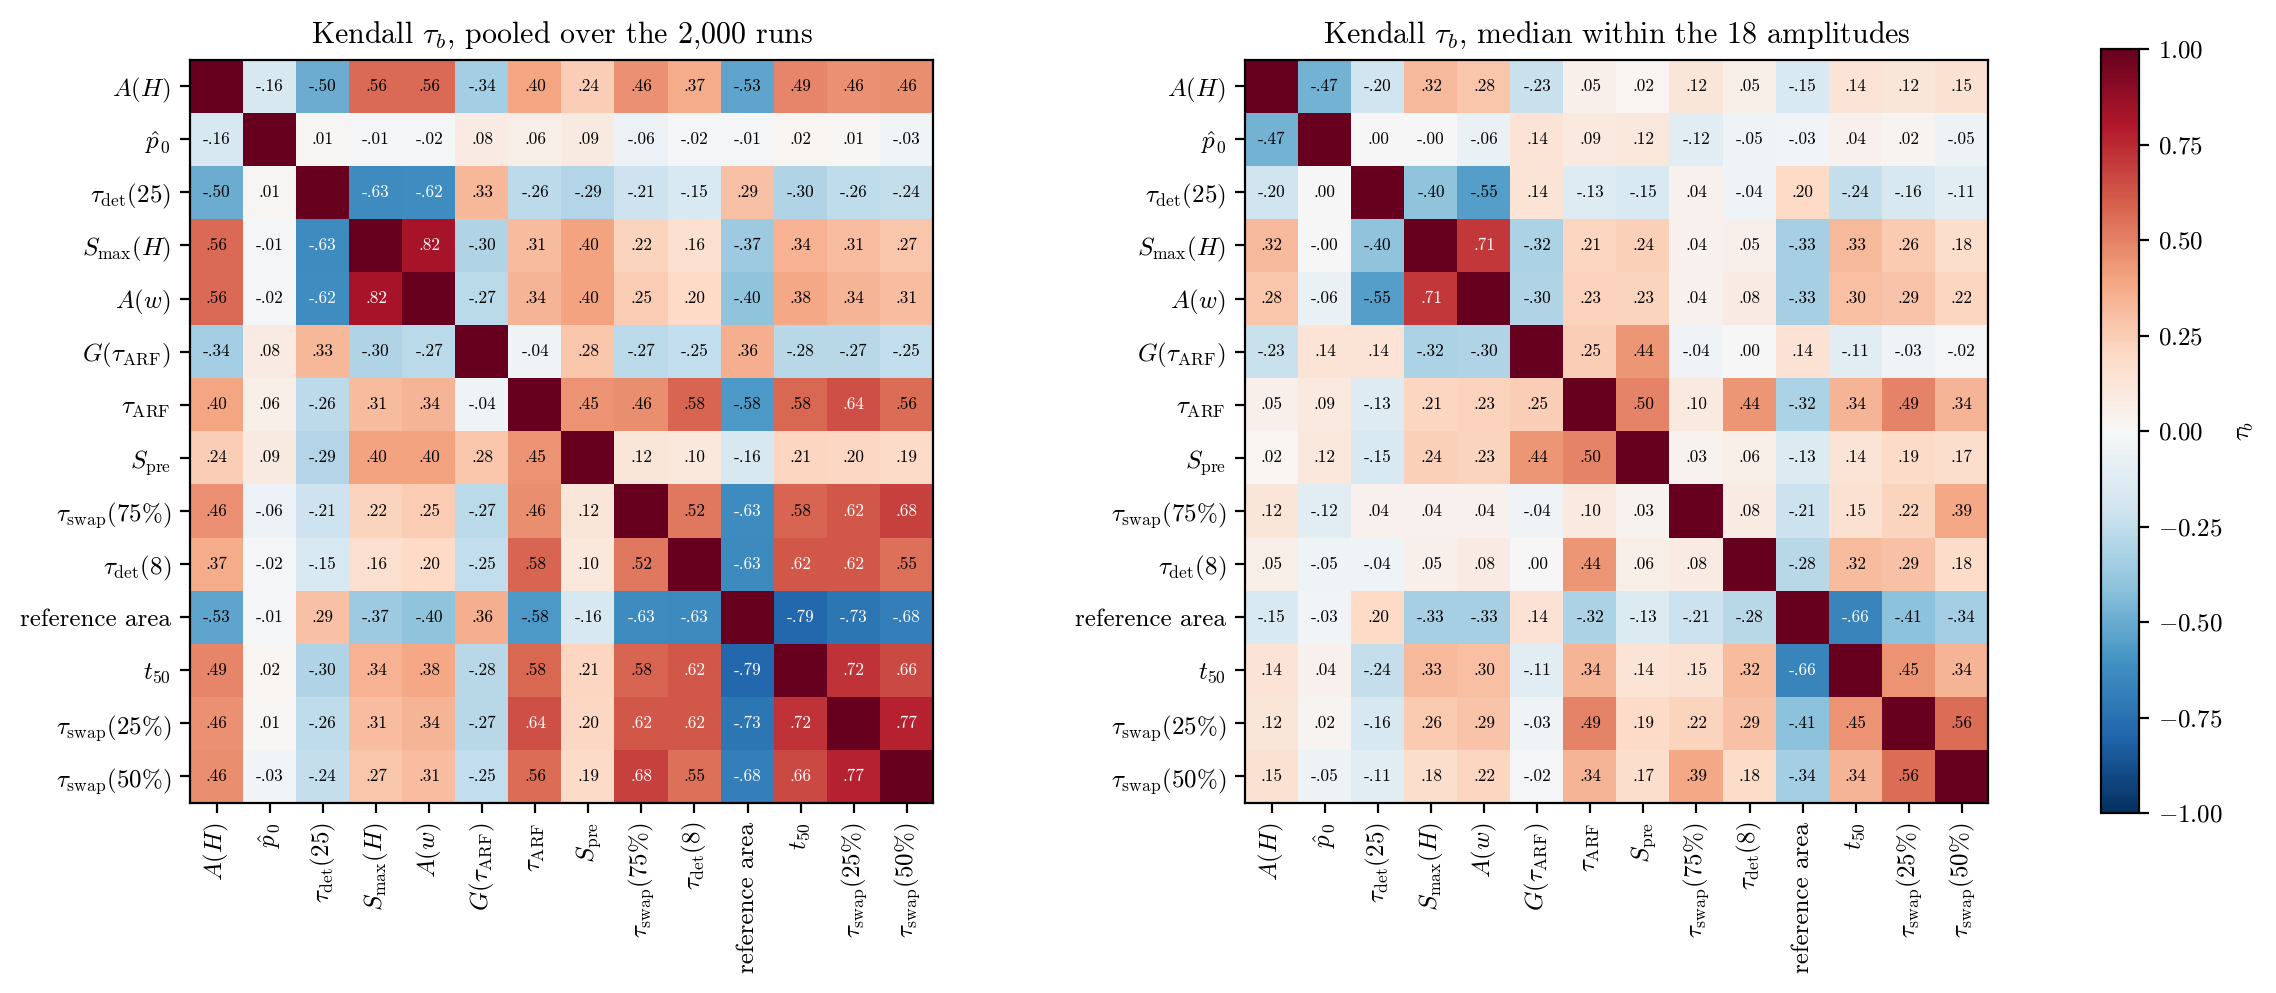
\includegraphics[width=0.86\textwidth]{Fig_QD_matrice_correlations_full.png}
  \end{center}
  \vspace{-0.5em}
  \small
  \begin{columns}[T,onlytextwidth]
    \begin{column}{0.32\textwidth}
      \textbf{Left, pooled:} almost everything agrees, because the drift size moves every
      indicator.
    \end{column}\hfill
    \begin{column}{0.32\textwidth}
      \textbf{Right, within a size:} two groups remain, \emph{evidence} ($0.71$) and
      \emph{repair}, weakly joined.
    \end{column}\hfill
    \begin{column}{0.32\textwidth}
      Best date against the analytic reference: \alert{3 trees replaced}, $0.45$, ahead of
      the first tree, $0.34$.
    \end{column}
  \end{columns}
  \note{To see all indicators at once, we crossed fourteen of them. The left panel pools all
    runs together: almost everything is strongly correlated with everything. That is an
    illusion, Simpson's paradox: the drift size moves every indicator, so pooling creates
    agreement. The right panel computes the same correlations within each drift size. Most of
    the agreement disappears, and two groups remain. One group measures evidence and damage:
    the detector's peak and the excess error over the transition agree strongly. The other
    group measures the repair. Between the two groups, links stay weak. We also compared the
    replacement dates with an analytic reference, the accuracy of the forest on the region
    whose label changed. The date at which three trees are replaced tracks it better than the
    first tree. This matrix is exploratory.}
\end{frame}

% =====================================================================
\section{III. Evidence vs threshold}
% =====================================================================

\begin{frame}{Part III --- Evidence against the threshold}
  \begin{center}\carte{3}\end{center}
  \note{The third part ties the first two together.}
\end{frame}

\begin{frame}{The race is decided before the repair}
  \begin{columns}[c,onlytextwidth]
    \begin{column}{0.52\textwidth}
      \centering
      \resizebox{\linewidth}{!}{\schemaidentite}\\
      {\scriptsize\color{gray} schematic}
    \end{column}\hfill
    \begin{column}{0.44\textwidth}
      A time counts observations; $\lambda$ counts \emph{excess errors}. Comparing them
      needs a rate that does not exist.
      \begin{block}{Race identity, on every run}
        \vspace{-0.4em}
        \[
          \tau_{\mathrm{det}} < \tau_{\mathrm{ARF}}
          \iff S_{\mathrm{pre}} \ge \lambda
        \]
        \vspace{-0.9em}
        \[
          S_{\mathrm{pre}} = \max_{t < \tau_{\mathrm{ARF}}} S_t
        \]
      \end{block}
      \small No rate, no averaging, no assumption on the trees. Checked on $2\,000$ runs out
      of $2\,000$ at three thresholds.
    \end{column}
  \end{columns}
  \note{Here is the key step. A repair time counts observations. A threshold counts excess
    errors. They are not in the same unit, and the paper bridges them with an average rate of
    errors per step. That rate does not exist: it falls as the forest repairs, and the
    detector forgets its evidence each time it hits zero. The exact statement is much
    simpler. Look at the statistic of the detector up to the first replacement, and take its
    highest point: we call it S pre. The detector arrives first if and only if S pre reaches
    the threshold. With a low threshold, it is reached before the repair; with a high one, it
    is not. This is exact on every run, it needs no rate, no averaging and no assumption on
    the trees, and we checked it on all two thousand runs.}
\end{frame}

\begin{frame}{The evidence before the repair sets the transition}
  \begin{columns}[c,onlytextwidth]
    \begin{column}{0.60\textwidth}
      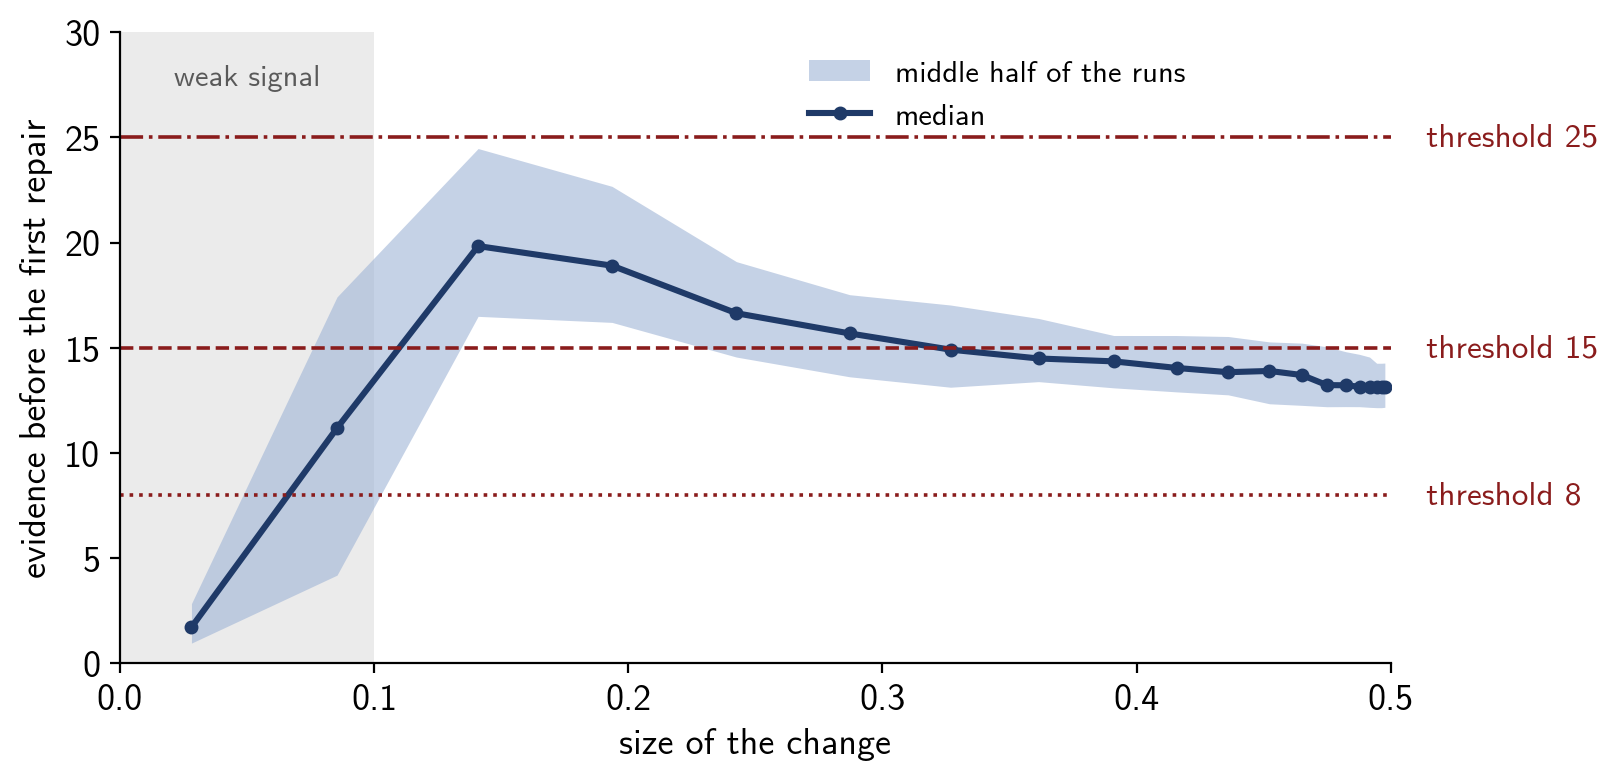
\includegraphics[width=\textwidth]{Fig_slide_spre.png}
    \end{column}\hfill
    \begin{column}{0.37\textwidth}
      \begin{itemize}
        \item Above the weak-signal zone, the median lies between \textbf{$13.1$ and $19.8$}:
              the transition the paper sees between $15$ and $25$, \alert{and leaves
              unexplained}.
        \item It \textbf{decreases} as the drift grows: at $\lambda = 15$ the detector wins
              $81\%$, then only $18\%$. That is the paradox.
      \end{itemize}
    \end{column}
  \end{columns}
  \note{So we measured S pre on every run. The dark line is the median by drift size, the band
    holds the middle half of the runs, and the red lines are thresholds. Above the weak-signal
    zone, the median sits between thirteen and twenty. A threshold below that level is reached
    before the repair in most runs; a threshold above it rarely is. That is exactly the
    transition the paper observes between fifteen and twenty-five, and leaves to future work.
    Now look at the shape. After the medium drifts, S pre decreases as the drift gets stronger,
    because the first replacement comes sooner. At a fixed threshold of fifteen, the detector
    wins eighty-one percent of the races on medium drifts, and only eighteen percent on the
    strongest ones. The paradox is this decreasing evidence, read against a fixed threshold. At
    the far left, the drift is too weak to accumulate anything: that is a different regime.}
\end{frame}

\begin{frame}{Stronger drifts leave no more evidence}
  \begin{columns}[c,onlytextwidth]
    \begin{column}{0.48\textwidth}
      \centering
      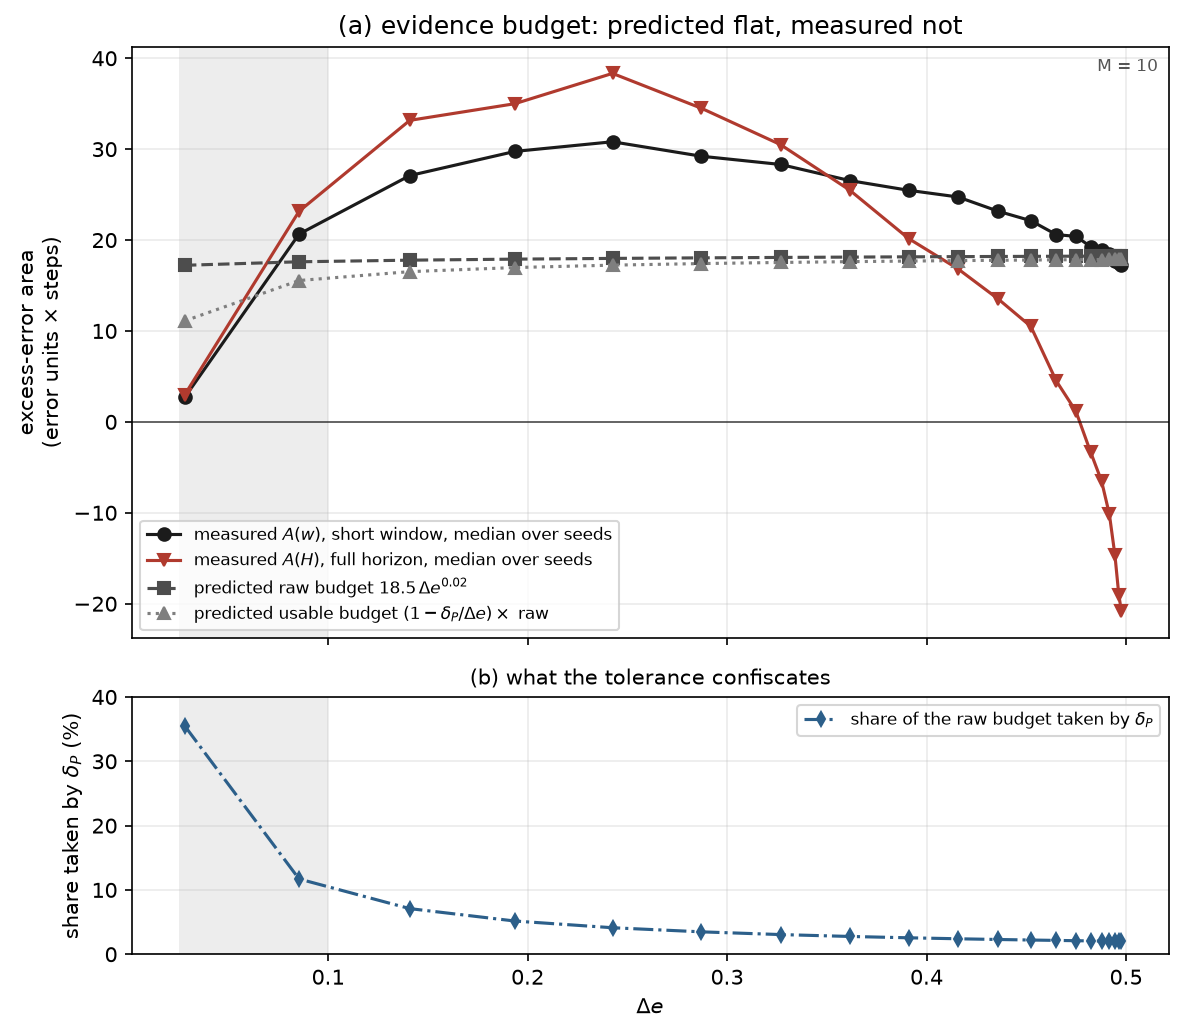
\includegraphics[height=0.66\textheight]{Fig_QC_budget_utilisable_full.png}
    \end{column}\hfill
    \begin{column}{0.46\textwidth}
      \begin{itemize}
        \item The paper's picture: an excess error $\Delta e$ over a window $\tau_{\mathrm{ARF}}$,
              so the area stays almost constant.
        \item Measured over the transition, the area varies by a factor of $1.8$ while the
              drift size varies by $5.8$: \alert{the compensation is real}.
        \item But the paper's rectangle misestimates it by up to $43\%$, and over the whole
              horizon the area turns negative at large drifts: the new task is easier.
      \end{itemize}
    \end{column}
  \end{columns}
  \note{Why doesn't a violent drift leave more evidence than a gentle one? The paper's picture
    is a rectangle: an excess error of height delta e, during a window equal to the repair
    time. Since the repair time shrinks like one over delta e, the area stays almost constant.
    We measured the area directly. Over the transition, it varies by a factor of less than two,
    while the drift size varies by almost six: the compensation is real. But the rectangle
    itself is wrong. It misestimates the area by up to forty-three percent, because the first
    replacement is not the width of the transient. And over the whole horizon, at large drifts,
    the area even becomes negative: after the change the task is easier than before, and the
    error settles below its old level. The evidence exists, it is roughly constant, but the
    paper's derivation of it does not hold.}
\end{frame}

\begin{frame}{Detecting is not winning}
  \begin{center}
    \begin{tabular}{@{}cccc@{}}
      \toprule
      threshold $\lambda$ & alarm fires & detector arrives first & false alarms, no drift \\
      \midrule
      $8$  & $95.3\%$ & $\mathbf{91.0\%}$ & $4.15\%$ \\
      $15$ & $92.9\%$ & $\mathbf{36.3\%}$ & $0.15\%$ \\
      $20$ & $66.2\%$ & $8.1\%$           & $0.00\%$ \\
      $25$ & $38.9\%$ & $2.5\%$           & $0.00\%$ \\
      \bottomrule
    \end{tabular}\\[0.3em]
    {\scriptsize\color{gray} $2\,000$ runs with drift and $2\,000$ without, over $2\,000$ steps}
  \end{center}
  \begin{itemize}
    \item At $\lambda = 15$ the alarm almost always fires, but mostly \emph{after} the repair.
    \item At $\lambda = 8$ the detector wins at an ordinary false-alarm cost: the paper's
          ``no threshold escapes'' does not hold on this bench.
    \item \textcolor{gray}{Not tested: the heteroscedastic streams where the paper places its
          false-alarm tension.}
  \end{itemize}
  \note{One practical consequence. Detecting a drift and winning the race are two different
    things. At threshold fifteen, the alarm fires on ninety-three percent of drifts, which
    looks excellent, but it arrives before the repair in only thirty-six percent of them.
    Most of these alarms come after the forest has already changed. At threshold eight, the
    detector wins ninety-one percent of the races, and it costs about four percent of false
    alarms over two thousand steps where nothing happens, which is an ordinary calibration
    level. So on this bench, one threshold does escape the blind spot, and the paper's claim
    that no threshold escapes has to be restricted. We did not test the financial streams
    with clustered volatility, where the paper places the false-alarm problem.}
\end{frame}

% =====================================================================
\section{Conclusion}
% =====================================================================

\begin{frame}{What changes in the paper}
  \small
  \begin{tabular}{@{}p{0.34\textwidth}p{0.43\textwidth}l@{}}
    \toprule
    The paper & Our result & \\
    \midrule
    races the repair against a constant & race identified, bounded, decided run by run & \textbf{made exact} \\
    independent trees, bias asserted & direction proven, cannot reverse & \textbf{proven} \\
    error back to normal at the first replacement & it comes back later; the rectangle fails & \textbf{corrected} \\
    first replacement as the repair date & earliest date, fires without drift & \textbf{qualified} \\
    transition between $15$ and $25$, unexplained & set by the evidence before the repair & \textbf{explained} \\
    no threshold escapes & $\lambda = 8$ does, on this bench & \textbf{restricted} \\
    \bottomrule
  \end{tabular}
  \vspace{0.6em}
  \begin{center}
    \alert{The phenomenon survives. What changes is its mechanism and its reach.}
  \end{center}
  \note{To sum up what our work changes in the paper. The race, which compared a random time
    with a constant, is made exact: identified, bounded, and decided run by run. The bias of
    the independence assumption was asserted; it is now proven, with its direction. The idea
    that the error is back to normal at the first replacement is corrected. The first
    replacement as a repair date is qualified: it is the earliest date and it fires without
    drift. The transition threshold, which the paper left unexplained, is explained by the
    evidence before the repair. And the claim that no threshold escapes is restricted to the
    settings the paper actually tested. The phenomenon survives all of this. What changes is
    its mechanism, and its reach.}
\end{frame}

\begin{frame}{An open question, and what we did not do}
  \begin{columns}[T,onlytextwidth]
    \begin{column}{0.50\textwidth}
      \begin{exampleblock}{Open: a reference for adaptation}
        Every indicator on the detector's side reads the \emph{error}, which mixes what the
        forest relearned with how hard the new task is. On analytic probes, the forest can
        relearn the changed region and lose a rare one, unseen by the error.
      \end{exampleblock}
    \end{column}\hfill
    \begin{column}{0.46\textwidth}
      \begin{block}{Not done}
        \small
        \begin{itemize}
          \item one forest size, one homoscedastic bench
          \item decision rule fixed during the analysis
          \item the independence bias has a sign, not a size
        \end{itemize}
      \end{block}
    \end{column}
  \end{columns}
  \note{We leave one question open. Every measure available to the detector reads the error,
    and the error mixes two things: what the forest has relearned, and how hard the new task
    is. Using analytic probes, points whose true label we know, we saw that the forest can
    relearn the region that changed while losing a rare region elsewhere, and the error does
    not see that loss. So what would a true reference for adaptation be? We do not have the
    answer. And to be honest about the limits: we studied one forest size on one simple
    bench, our decision rule was fixed during the analysis rather than before it, and we can
    give the sign of the independence bias but not its size.}
\end{frame}

\begin{frame}{Take-away}
  \begin{center}
    \small\alert{The blind spot is a budget of evidence, accumulated before the repair, set
    against a threshold.}
  \end{center}
  \vspace{-0.5em}
  \begin{center}\carte[0.71]{0}\end{center}
  \note{Back to the map. The blind spot is real, and it survives every correction. But it is
    not a race between two clocks. It is the evidence the forest lets through before its first
    repair, set against a fixed threshold. That single quantity explains when the detector
    wins, why the transition sits where it does, and why stronger drifts are missed more
    often. Thank you for your attention; we are happy to take your questions.}
\end{frame}

% =====================================================================
\appendix
\section*{Backup}
% =====================================================================

\begin{frame}{Backup --- Fréchet bounds}
  For integer-valued clocks with marginal CDFs $F_A$ and $F_D$, and \emph{any} coupling,
  \begin{align*}
    P_{\mathrm{miss}} &\ge \max\Big(0,\ \sup_{s} \big[F_A(s)-F_D(s)\big]\Big),\\
    P_{\mathrm{miss}} &\le \min\Big(1,\ \inf_{s} \big[F_A(s) + 1 - F_D(s+1)\big]\Big).
  \end{align*}
  \begin{itemize}
    \item Lower: Fréchet on $\{\tau_{\mathrm{ARF}} \le s < \tau_{\mathrm{det}}\} \subseteq \mathrm{Miss}$.
    \item Upper: $\mathrm{Miss} \subseteq \{\tau_{\mathrm{ARF}} \le s\} \cup \{\tau_{\mathrm{det}} > s+1\}$, then Boole.
    \item Toy case, both clocks uniform on $\{1,2\}$: the bounds $0$ and $0.5$ are both attained.
  \end{itemize}
\end{frame}

\begin{frame}{Backup --- Lindley's closed form and the certificate}
  With $X_t = e_t - \hat p_0 - \delta_P$ and $A(k,j) = \sum_{t=k+1}^{j} (e_t - \hat p_0)$,
  \[
    S_j = \max_{0 \le k \le j} \sum_{t=k+1}^{j} X_t,
    \qquad
    S_{\max}(H) = \max_{0 \le k \le j \le H} \big[A(k,j) - (j-k)\,\delta_P\big].
  \]
  \begin{itemize}
    \item Certificate: the alarm fires by $H$ iff some sub-window carries
          $A(k,j) \ge \lambda + (j-k)\,\delta_P$. The full window alone is only sufficient.
    \item Race identity: the same maximum, taken up to the first replacement, is $S_{\mathrm{pre}}$.
  \end{itemize}
\end{frame}

\begin{frame}{Backup --- Association protocol}
  \begin{itemize}
    \item Every coefficient is computed \textbf{within a drift size} ($100$ seeds), on the $18$
          sizes with $\Delta e \ge 0.10$: pooling measures the drift size, not the link.
    \item Kendall's $\tau_b$: reads on pairs, corrects for ties. Censored durations ranked last,
          licit because the horizon is common to all runs.
    \item Pearson undefined on censored values; Spearman handles their ties implicitly.
    \item Percentile bootstrap over seeds, $2\,000$ resamples; discernible if the interval
          excludes zero. Fixed during the analysis, not before: stated in the report.
    \item Complete cases instead of ranking censored runs last: no coefficient moves by more
          than $0.0403$.
  \end{itemize}
\end{frame}

\begin{frame}{Backup --- The drift-free control}
  \begin{center}
    \begin{tabular}{@{}lr@{}}
      \toprule
      On $2\,000$ runs with no change point & \\
      \midrule
      runs where at least one tree is replaced & $2\,000/2\,000$ \\
      first replacement, median & $95$ steps \\
      distinct trees renewed, median & $9/10$ \\
      forest entirely renewed & $28.7\%$ \\
      \midrule
      first replacement at the weakest drift, median & $118$ steps \\
      \bottomrule
    \end{tabular}
  \end{center}
\end{frame}

\end{document}
"
%
% Tracabilite : chaque chiffre vient du rapport ; controle par
%   verif_chiffres_tex.py ../../05_presentation/soutenance_20min.tex
% Figures : figures_slides.py --latex, figures_soutenance.py,
%   matrice_correlations.py, analyse_QCD.py (budget).
% =====================================================================

\documentclass[aspectratio=169,11pt]{beamer}

\usetheme{Madrid}
% Rouge de CentraleSupelec, pris dans le logo officiel (#B00739) ; logo
% CentraleSupelec / Universite Paris-Saclay sur la page de titre.
\definecolor{csRouge}{HTML}{B00739}
\usecolortheme[named=csRouge]{structure}
\setbeamercolor{alerted text}{fg=csRouge}
\setbeamersize{text margin left=1cm, text margin right=1cm}
\setbeamertemplate{navigation symbols}{}
\usepackage[english]{babel}
\usepackage{amsmath,amssymb}
\usepackage{graphicx}
\usepackage{booktabs}
\usepackage{tikz}
% soutenance_schemas.tex
% =====================================================================
% Schemas TikZ de `soutenance_20min.tex` : la carte des idees et le schema
% de l'identite de course.
%
% Fichier separe pour la meme raison que `point_encadrant_schemas.tex` :
% `verif_chiffres_tex.py` ramasserait les coordonnees TikZ comme des mesures.
% AUCUN chiffre de mesure ici ; les schemas sont stylises, sans donnees.
% =====================================================================

\usetikzlibrary{positioning, arrows.meta, calc}

\definecolor{mTheorie}{RGB}{31,58,104}
\definecolor{mDate}{RGB}{138,28,28}
\definecolor{mPreuve}{RGB}{38,92,58}
\definecolor{mEteint}{gray}{0.74}

% ---------------------------------------------------------------------
% \carte[hauteur]{k} : la carte des idees.
%   k = 0 : tout est actif (ouverture et conclusion)
%   k = 1, 2, 3 : seule la partie k est en couleur, le reste est grise
%   hauteur : fraction de \textheight (0.80 par defaut)
% Les fleches en pointille relient les parties ; elles sont commentees a
% l'oral plutot qu'etiquetees, faute de place entre les colonnes.
% ---------------------------------------------------------------------
\newcommand{\carte}[2][0.80]{%
  \colorlet{cUn}{mEteint}\colorlet{cDeux}{mEteint}\colorlet{cTrois}{mEteint}%
  \colorlet{tUn}{mEteint}\colorlet{tDeux}{mEteint}\colorlet{tTrois}{mEteint}%
  \ifnum#2=0 \colorlet{cUn}{mTheorie}\colorlet{cDeux}{mDate}\colorlet{cTrois}{mPreuve}%
    \colorlet{tUn}{black}\colorlet{tDeux}{black}\colorlet{tTrois}{black}\fi
  \ifnum#2=1 \colorlet{cUn}{mTheorie}\colorlet{tUn}{black}\fi
  \ifnum#2=2 \colorlet{cDeux}{mDate}\colorlet{tDeux}{black}\fi
  \ifnum#2=3 \colorlet{cTrois}{mPreuve}\colorlet{tTrois}{black}\fi
  \resizebox{!}{#1\textheight}{%
  \begin{tikzpicture}[
      font=\normalsize, align=center,
      boite/.style={draw, line width=1pt, rounded corners=3pt, inner sep=4pt,
                    text width=4.3cm, minimum height=1.05cm},
      un/.style={boite, draw=cUn, text=tUn},
      deux/.style={boite, draw=cDeux, text=tDeux},
      trois/.style={boite, draw=cTrois, text=tTrois},
      tete/.style={font=\bfseries\normalsize, text width=4.8cm},
      fl/.style={-{Stealth[length=2.4mm]}, line width=0.9pt},
      lien/.style={-{Stealth[length=2.4mm]}, line width=0.9pt, dashed},
    ]
    \node[boite, draw=black, fill=black!4, text width=12cm, minimum height=0.8cm] (P) at (5.6,0.15)
      {\textbf{The paper:} the stronger the drift, the faster the repair, the fewer the alarms};

    \node[tete, text=cUn]    (H1) at (0,-1.05)    {I.\ The race, formally};
    \node[tete, text=cDeux]  (H2) at (5.6,-1.05)  {II.\ The repair date};
    \node[tete, text=cTrois] (H3) at (11.2,-1.05) {III.\ Evidence vs threshold};
    \draw[fl, black!55] (P.south) -- ++(0,-0.25) -| (H1.north);
    \draw[fl, black!55] (P.south) -- (H2.north);
    \draw[fl, black!55] (P.south) -- ++(0,-0.25) -| (H3.north);

    \node[un] (A1) at (0,-2.1)  {The miss is well defined, its probability identified};
    \node[un] (A2) at (0,-3.45) {The blind spot holds whatever the dependence};
    \node[un] (B1) at (0,-4.8)  {Independent trees overstate the speed of repair};

    \node[deux] (C1) at (5.6,-2.1)  {The first replacement is the earliest date};
    \node[deux] (E1) at (5.6,-3.45) {It fires as fast when nothing changes};
    \node[deux] (D1) at (5.6,-4.8)  {When it fires, half the evidence is there};
    \node[deux] (D2) at (5.6,-6.15) {Indicators form two groups, weakly linked};

    \node[trois] (C2) at (11.2,-2.1)  {The alarm is a function of the error path};
    \node[trois] (K)  at (11.2,-3.45) {Detector first \emph{iff} it reaches $\lambda$ before the repair};
    \node[trois] (S)  at (11.2,-4.8)  {That evidence sets the transition and the paradox};
    \node[trois] (T)  at (11.2,-6.15) {Detecting is not winning};

    \node[boite, draw=black!55, text=black!80, dashed, text width=7cm, minimum height=0.8cm] (O) at (5.6,-7.45)
      {\textbf{Open:} a reference for adaptation itself};

    \draw[fl, cUn]    (A1) -- (A2);
    \draw[fl, cDeux]  (C1) -- (E1);
    \draw[fl, cDeux]  (E1) -- (D1);
    \draw[fl, cDeux]  (D1) -- (D2);
    \draw[fl, cTrois] (C2) -- (K);
    \draw[fl, cTrois] (K) -- (S);
    \draw[fl, cTrois] (S) -- (T);
    \draw[lien, black!55] (B1.east) -- (D1.west);
    \draw[lien, black!55] (D1.east) -- (S.west);
    \draw[lien, black!55] (D2.south) -- (O.north);
  \end{tikzpicture}}%
}

% ---------------------------------------------------------------------
% \schemaidentite : la pile S_t, le premier remplacement, deux seuils.
% Stylise, sans donnees.
% ---------------------------------------------------------------------
\newcommand{\schemaidentite}{%
  \begin{tikzpicture}[x=1cm, y=1cm, font=\small]
    \draw[-{Stealth}, line width=0.7pt] (0,0) -- (7.2,0);
    \node[below left] at (7.2,-0.05) {time};
    \draw[-{Stealth}, line width=0.7pt] (0,0) -- (0,3.7);
    \node[rotate=90, above] at (-0.05,1.85) {detector statistic $S_t$};
    \draw[line width=1.4pt, mTheorie]
      (0,0) .. controls (0.8,0.6) and (1.6,1.9) .. (2.4,2.25)
            .. controls (3.0,2.5) and (3.4,2.55) .. (3.9,2.4)
            .. controls (4.8,2.0) and (5.8,1.0) .. (7.0,0.3);
    \draw[dashed, mDate, line width=1pt] (2.8,0) -- (2.8,3.4);
    \node[above, text=mDate] at (2.8,3.4) {first replacement};
    \fill[mTheorie] (2.8,2.38) circle (2.3pt);
    \node[above left, text=mTheorie] at (2.75,2.4) {$S_{\mathrm{pre}}$};
    \draw[mPreuve, line width=1pt] (0,1.5) -- (7.0,1.5);
    \node[above left, text=mPreuve] at (7.0,1.5) {low $\lambda$: reached before};
    \draw[mDate, line width=1pt, dash dot] (0,3.0) -- (7.0,3.0);
    \node[above left, text=mDate] at (7.0,3.0) {high $\lambda$: not reached};
  \end{tikzpicture}%
}

\titlegraphic{
\includegraphics[height=1.7cm]{Logo_CS_Paris_Saclay.png}}
\ifdefined\NOTESSEULES\setbeameroption{show only notes}\fi
\graphicspath{{../04_experimentations/resultats_R2/resultats/figures/slides_latex/}{../04_experimentations/resultats_R2/resultats/figures/}}

\setbeamerfont{author}{size=\small}
\setbeamerfont{institute}{size=\scriptsize}

\title[The Blind Spot Paradox]{The Blind Spot Paradox}
\subtitle{Formalizing the race and measuring the adaptation}
\author[Boyer, Gouillou, Fonvielle, Petit-Tichanné]{Alexandre Boyer \and Melaine Gouillou \and Salomé Fonvielle \and Ulysse Petit-Tichanné}
\institute[CS]{Research Track, Topic 39, CentraleSupélec. Supervisor: Raphaël Minato}
\date{16 September 2026}

\begin{document}

\maketitle
\note{Good afternoon. Our subject is the blind spot paradox: a model that repairs
  itself can destroy the very evidence its own monitor needs. In the next twenty
  minutes we will present what we formalized, what we measured, and the single
  reading that ties the two together.}

% =====================================================================
\section{The problem}
% =====================================================================

\begin{frame}{Concept drift: the rule changes, the data does not}
  \vspace{-0.6em}
  \[
    \underbrace{P(X)}_{\text{the data}}\ \text{unchanged}
    \qquad\qquad
    \underbrace{P(Y \mid X)}_{\text{the rule}}\ \text{changes}
  \]
  \vspace{-0.9em}
  \begin{center}
    
\includegraphics[height=0.50\textheight]{Fig_slide_drift.png}
  \end{center}
  \begin{center}
    A model trained before the change is now \alert{wrong on the shaded band}.
  \end{center}
  \note{A classifier learns a rule from data. In a data stream, that rule can change
    while the inputs keep exactly the same distribution. This is concept drift: P of X
    does not move, P of Y given X does. It is the normal situation for a financial
    signal, where the same inputs stop meaning the same thing. In the bench we use,
    points in the plane are separated by a line. At the change, the line moves. Every
    point in the shaded band switches label, so a model trained before the change keeps
    predicting confidently, and is now wrong on that band. The size of the band is the
    size of the drift, written delta e.}
\end{frame}

\begin{frame}{Two defences that run at the same time}
  \begin{columns}[T,onlytextwidth]
    \begin{column}{0.49\textwidth}
      \centering
      \textbf{The model repairs itself}\\[0.3em]
      
\includegraphics[width=\textwidth]{Fig_slide_foret.png}\\[0.2em]
      \small Adaptive Random Forest: ten trees, each replaced when its own error rises.
    \end{column}\hfill
    \begin{column}{0.49\textwidth}
      \centering
      \textbf{A monitor raises the alarm}\\[0.3em]
      
\includegraphics[width=\textwidth]{Fig_slide_watchdog.png}\\[0.2em]
      \small Each error adds to a statistic $S_t$; the alarm fires when it crosses $\lambda$.
    \end{column}
  \end{columns}
  \note{Two defences are deployed together. The first one lives inside the model. The
    Adaptive Random Forest is made of ten decision trees that vote. Each tree watches its
    own error with a small detector, and when that error rises, the tree is replaced by a
    fresh one. The forest repairs itself locally, without asking anyone. The second defence
    sits outside. A cumulative detector, a Page-Hinkley test, watches the error of the
    whole forest. Every error pushes a statistic up by almost one, every correct answer
    pulls it down a little, never below zero. When the statistic crosses a threshold
    lambda, the alarm fires, and that alarm is the only thing a human operator sees.}
\end{frame}

\begin{frame}{The paradox, and what the reviewers asked}
  \begin{columns}[c,onlytextwidth]
    \begin{column}{0.50\textwidth}
      \centering
      
\includegraphics[width=\textwidth]{Fig_slide_mecanisme.png}\\
      {\scriptsize\color{gray} schematic}
    \end{column}\hfill
    \begin{column}{0.46\textwidth}
      \begin{block}{The paper's claim}
        The stronger the drift, the faster the repair, and the \alert{fewer} alarms.
      \end{block}
      \begin{alertblock}{Two corrections requested}
        \begin{enumerate}
          \item It races a random repair time against a \emph{constant}, and assumes the
                trees independent.
          \item It dates the repair at the \emph{first} tree replaced, without showing
                that this date means anything.
        \end{enumerate}
      \end{alertblock}
    \end{column}
  \end{columns}
  \note{When both defences run together, something unexpected happens. The drift starts,
    errors pile up in the detector, but the forest replaces trees, the errors stop, and the
    pile drains before it reaches the threshold. The paper we study calls this the blind
    spot paradox: the stronger the drift, the faster the forest repairs itself, and the
    fewer alarms the operator gets. The paper was reviewed, and two corrections were
    requested. First, it compares a random repair time with a constant detection time, and
    it assumes the ten trees are independent without proving it. Second, it dates the repair
    at the moment the first tree is replaced, without showing that this moment has anything
    to do with the error disappearing. These two corrections are where our work starts.}
\end{frame}

\begin{frame}{Our reading, in one map}
  \begin{center}
    \small\alert{The blind spot is not a race between two clocks,
    but a budget of evidence set against a threshold.}
  \end{center}
  \vspace{-0.5em}
  \begin{center}
    \carte[0.71]{0}
  \end{center}
  \note{Here is the whole talk on one map. At the top, the claim of the paper. The first
    column formalizes the race: we define the blind spot properly, we compute its
    probability, and we show that assuming independent trees makes the paper optimistic
    about the repair. The second column asks what the repair date really measures: it is
    the earliest possible date, it fires even when nothing changes, and when it fires most
    of the evidence is already there. The third column ties both together: the detector wins
    exactly when its evidence reaches the threshold before the repair, and that evidence
    explains both the transition and the paradox. The dashed arrows are the links between
    columns, and the box at the bottom is the question we leave open. Our one-sentence
    reading: the blind spot is not a race between two clocks, it is a budget of evidence set
    against a threshold.}
\end{frame}

% =====================================================================
\section{I. The race}
% =====================================================================

\begin{frame}{Part I --- The race, formally}
  \begin{center}\carte{1}\end{center}
  \note{Let us start with the theory: how to state the race without cheating.}
\end{frame}

\begin{frame}{The race is well posed, and its probability identified}
  \begin{columns}[T,onlytextwidth]
    \begin{column}{0.46\textwidth}
      \begin{block}{One definition, no ad hoc rule}
        \[
          \mathrm{Miss} := \{\tau_{\mathrm{ARF}} < \tau_{\mathrm{det}}\}
        \]
        \vspace{-0.6em}
        {\small strict inequality; the alarm may never come}
        \begin{itemize}
          \item a tie goes to the detector
          \item a silent repair, with no alarm ever, \alert{is} a miss
          \item if neither acts, it is not
        \end{itemize}
      \end{block}
    \end{column}\hfill
    \begin{column}{0.50\textwidth}
      \begin{exampleblock}{What the campaign allows}
        The forest always replaces a tree within the horizon, so no run is left
        undecided: $P_{\mathrm{miss}}$ is \textbf{identified}.\\[0.3em]
        \centering
        \begin{tabular}{@{}lccc@{}}
          $\lambda$ & $8$ & $25$ & $50$ \\
          $P_{\mathrm{miss}}$ & $0.0905$ & $0.9715$ & $1.0000$
        \end{tabular}
      \end{exampleblock}
      \begin{alertblock}{Without any dependence assumption}
        From the marginal laws alone, the blind spot at the weakest drift is at least
        $0.91$ at $\lambda = 8$.
      \end{alertblock}
    \end{column}
  \end{columns}
  \note{The paper says there is a blind spot when the forest repairs before the alarm, but
    it quietly sets aside the runs where the alarm never comes. Those are exactly the runs
    where the detector fails most. So we define the event on the complete race, with one
    definition and no extra rule. A tie counts for the detector, because the operator is
    warned at the right moment. A silent repair, where the alarm never comes, is a miss, and
    in fact the purest one. A run where neither mechanism acts is not a miss, because there
    was nothing to erase. Then comes the problem of the finite horizon: some runs could be
    undecided. On our campaign they are not, because the forest always acts within the
    horizon, so the miss probability is identified exactly: nine percent at threshold eight,
    ninety-seven at twenty-five, one hundred at fifty. And with Fréchet bounds, which use the
    two marginal laws and assume nothing on how the clocks are coupled, the blind spot at the
    weakest drift is already forced above ninety percent.}
\end{frame}

\begin{frame}{Trees share a stream: the paper is optimistic}
  \begin{enumerate}
    \item \textbf{Given the stream}, what separates two trees is their own random draws:
          the trees are independent \emph{conditionally}.
    \item \textbf{Averaging over streams}, convexity gives the direction:
          \[
            P(\tau_{\mathrm{ARF}} \le s) \;\le\; 1 - \big(1 - F(s)\big)^M
          \]
          \alert{The independence formula overstates the speed of the repair.}
    \item \textbf{Consequence}: the paper's critical ensemble size becomes a conservative
          ceiling; its verdict does not change.
    \item \textbf{No coupling reverses the sign}: sharing a stream can only make trees fail
          together, since the covariance equals a variance.
  \end{enumerate}
  \note{The second shortcut is independence. The ten trees learn from the same stream, so
    they cannot be independent. But the question is at which level. Once the stream is
    fixed, what distinguishes one tree from another is only its own randomness, the random
    weights of online bagging. At that level, given the stream, the trees are independent.
    When we average over streams, Jensen's inequality gives a clear direction: the
    probability that the forest has already repaired itself is at most what the independence
    formula predicts. So the paper makes the forest look faster than it is, and overestimates
    the blind spot. Its critical ensemble size is not wrong, it becomes a conservative
    ceiling, and the paper's own verdict does not change. Could dependence go the other way?
    No: the covariance between two trees equals a variance, so it is never negative.}
\end{frame}

% =====================================================================
\section{II. The repair date}
% =====================================================================

\begin{frame}{Part II --- What the repair date measures}
  \begin{center}\carte{2}\end{center}
  \note{Now the second correction: the date the paper uses for the repair.}
\end{frame}

\begin{frame}{How we measured}
  \begin{columns}[T,onlytextwidth]
    \begin{column}{0.48\textwidth}
      \begin{block}{The campaign}
        \begin{itemize}
          \item the paper's bench, rerun: $20$ drift sizes $\times$ $100$ seeds,
                $2\,000$ steps after the change
          \item $2\,000$ more runs with no change at all
          \item only the error and the replacement events are recorded; every threshold is
                replayed offline
        \end{itemize}
      \end{block}
    \end{column}\hfill
    \begin{column}{0.48\textwidth}
      \begin{block}{Reading an association}
        \begin{itemize}
          \item always \alert{within one drift size}: pooling measures the drift size, not
                the link
          \item Kendall's rank correlation, with bootstrap intervals over the seeds
          \item steps added after seeing the data are flagged as exploratory
        \end{itemize}
      \end{block}
    \end{column}
  \end{columns}
  \note{A word on how we measured, without the implementation details. We reran the bench
    of the paper on twenty drift sizes, with one hundred seeds each, and we observe two
    thousand steps after the change. We added two thousand runs where nothing changes at
    all, as a control. The simulation records only two things: the error at each step and
    the moments when trees are replaced. Everything else, including the detector at any
    threshold, is recomputed offline, so one campaign replaces many. When we correlate two
    quantities, we always do it within one drift size. The drift size moves every indicator
    at once, so a correlation pooled over sizes mostly measures the size itself. We use
    Kendall's rank correlation with bootstrap intervals, and we flag the steps we added
    after looking at the data.}
\end{frame}

\begin{frame}{The first replacement is the earliest possible date}
  \begin{center}
    
\includegraphics[width=0.90\textwidth]{Fig_slide_deux_horloges.png}
  \end{center}
  \vspace{-0.3em}
  \begin{itemize}
    \item On every run, the first replacement comes before any other quota of renewed
          trees. Three quarters of the forest are renewed \textbf{$6.0$ to $14.3$ times later}.
    \item \alert{With no drift at all}, the first replacement comes after $95$ steps in
          median, against $118$ on the weakest drift.
  \end{itemize}
  \note{The paper dates the repair at the first replaced tree. By construction, that is the
    earliest of all possible dates: the moment when three trees, or half, or three quarters
    of the forest are replaced, always comes later, on every run. The only question is how
    much later. On this medium drift, the first tree goes after eighty-six observations, and
    three quarters of the forest after more than twelve hundred. Over the grid, three
    quarters of the forest are renewed six to fourteen times later than the first tree. And
    there is a more worrying fact. On the two thousand runs with no change at all, the forest
    still replaces its first tree, after ninety-five steps in median. On the weakest real
    drift, it takes one hundred and eighteen. So at low drift, this date cannot tell a real
    change from noise.}
\end{frame}

\begin{frame}{When the first tree goes, most of the evidence is already there}
  \begin{columns}[T,onlytextwidth]
    \begin{column}{0.36\textwidth}
      \begin{block}{Evidence at the first replacement}
        \centering
        {\Large $49\%$ to $76\%$}\\[0.2em]
        \small of the detector's final peak, on the $18$ drift sizes studied
      \end{block}
    \end{column}\hfill
    \begin{column}{0.60\textwidth}
      \begin{block}{Does the date track anything, within a drift size?}
        \small
        \begin{tabular}{@{}lcc@{}}
          \toprule
          compared with & median link & sizes \\
          \midrule
          detector peak & $0.21$ & $15/18$ \\
          excess error, whole horizon & none & $0/18$ \\
          excess error, transition only & $0.23$ & $13/18$ \\
          \bottomrule
        \end{tabular}
      \end{block}
    \end{column}
  \end{columns}
  \vspace{0.8em}
  \begin{center}
    \small The null over the whole horizon is mostly noise: \alert{half} of that area's
    variance comes from the estimated baseline, multiplied by the horizon.
  \end{center}
  \note{Is the first replacement at least the end of the transient? No. When the first tree
    is replaced, the detector already holds between half and three quarters of all the
    evidence it will ever accumulate. The replacement is in the middle of the story, not at
    its end. Then we asked whether this date tracks anything, always within a drift size.
    With the peak of the detector, there is a weak but real link, visible on fifteen drift
    sizes out of eighteen. With the excess error over the whole horizon, there is no link at
    all. But we found out why: that area adds up two thousand steps, so any error on the
    baseline is multiplied by two thousand, and half of its variance is just that noise. If
    we keep only the transition, the link comes back, weak but real, on thirteen sizes out of
    eighteen. This last step is exploratory.}
\end{frame}

\begin{frame}{Unexpected: pooling manufactures agreement}
  \begin{center}
    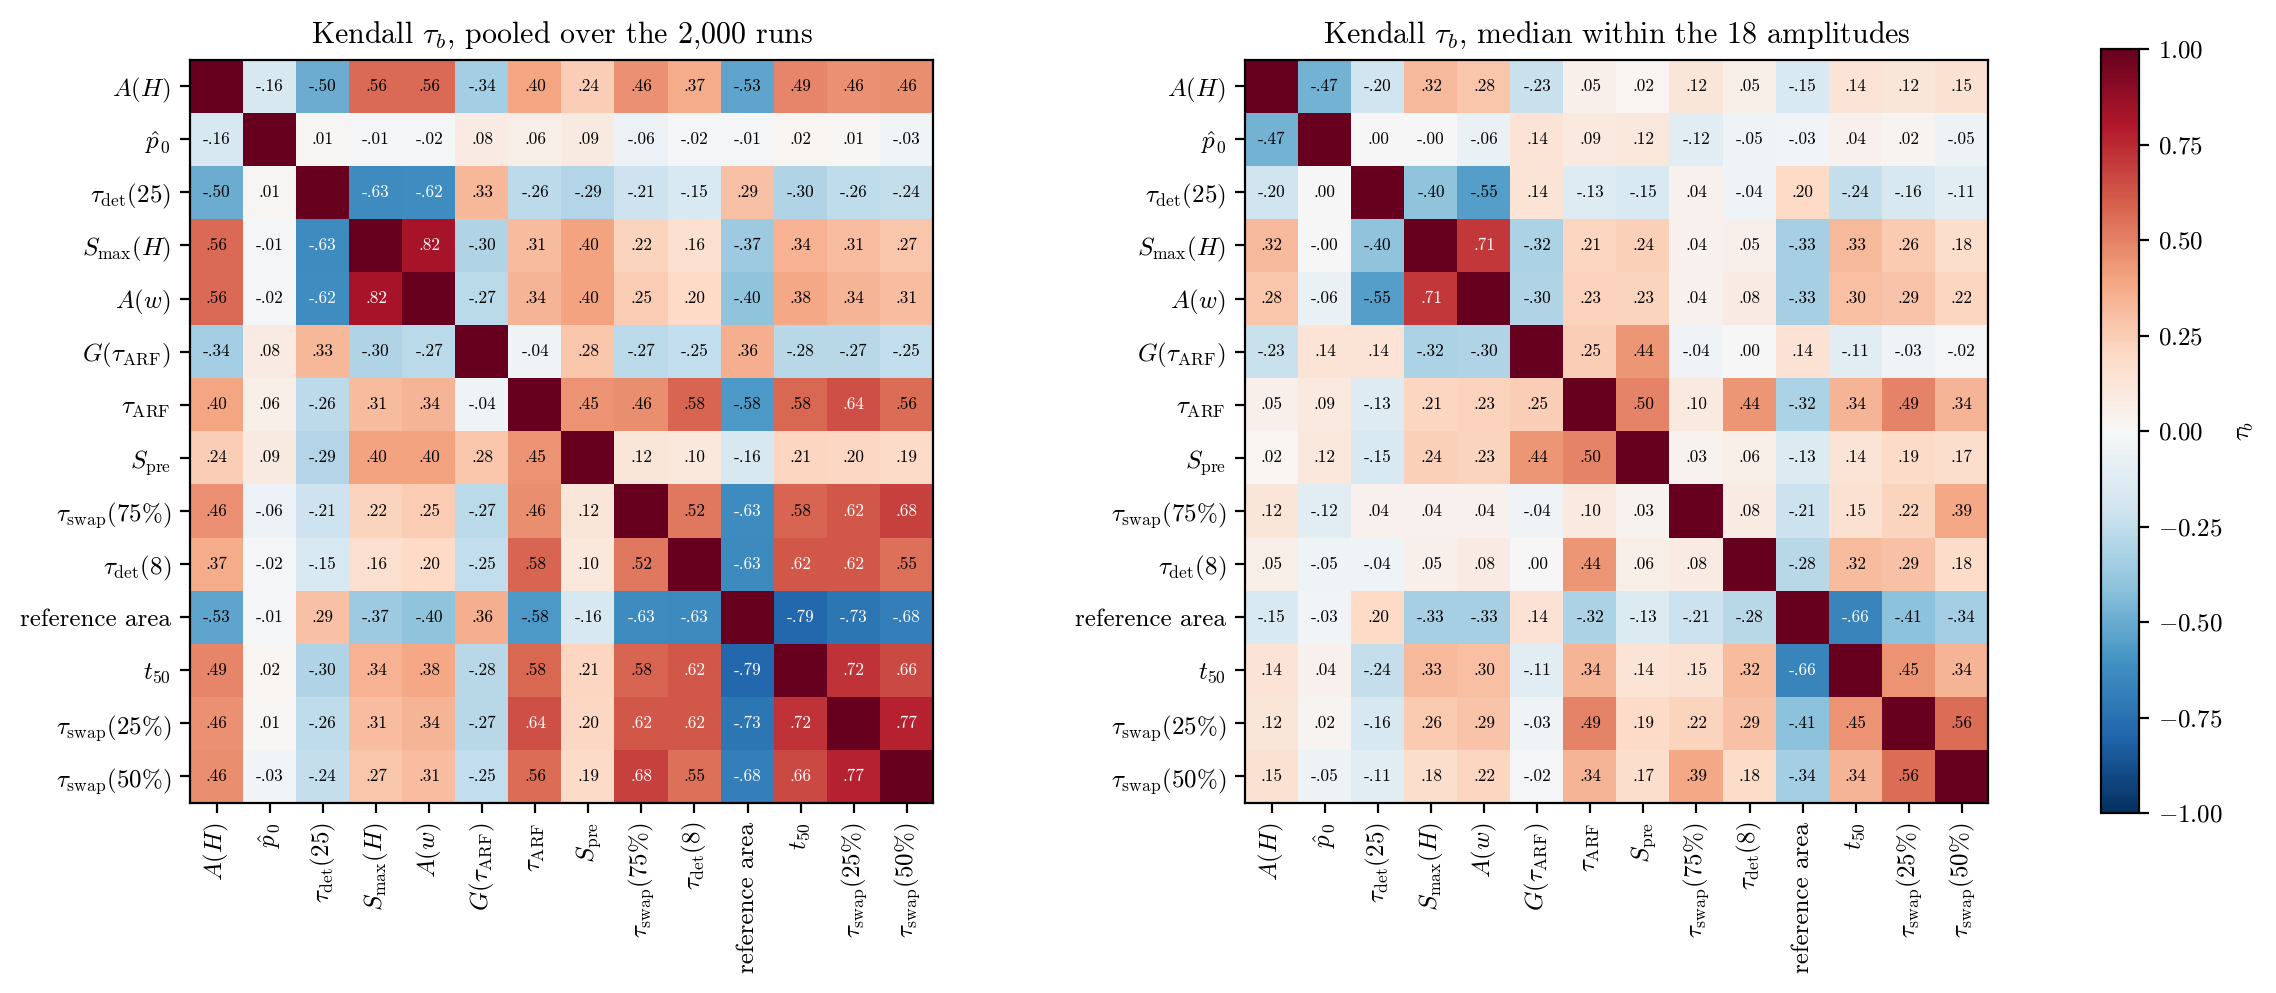
\includegraphics[width=0.86\textwidth]{Fig_QD_matrice_correlations_full.png}
  \end{center}
  \vspace{-0.5em}
  \small
  \begin{columns}[T,onlytextwidth]
    \begin{column}{0.32\textwidth}
      \textbf{Left, pooled:} almost everything agrees, because the drift size moves every
      indicator.
    \end{column}\hfill
    \begin{column}{0.32\textwidth}
      \textbf{Right, within a size:} two groups remain, \emph{evidence} ($0.71$) and
      \emph{repair}, weakly joined.
    \end{column}\hfill
    \begin{column}{0.32\textwidth}
      Best date against the analytic reference: \alert{3 trees replaced}, $0.45$, ahead of
      the first tree, $0.34$.
    \end{column}
  \end{columns}
  \note{To see all indicators at once, we crossed fourteen of them. The left panel pools all
    runs together: almost everything is strongly correlated with everything. That is an
    illusion, Simpson's paradox: the drift size moves every indicator, so pooling creates
    agreement. The right panel computes the same correlations within each drift size. Most of
    the agreement disappears, and two groups remain. One group measures evidence and damage:
    the detector's peak and the excess error over the transition agree strongly. The other
    group measures the repair. Between the two groups, links stay weak. We also compared the
    replacement dates with an analytic reference, the accuracy of the forest on the region
    whose label changed. The date at which three trees are replaced tracks it better than the
    first tree. This matrix is exploratory.}
\end{frame}

% =====================================================================
\section{III. Evidence vs threshold}
% =====================================================================

\begin{frame}{Part III --- Evidence against the threshold}
  \begin{center}\carte{3}\end{center}
  \note{The third part ties the first two together.}
\end{frame}

\begin{frame}{The race is decided before the repair}
  \begin{columns}[c,onlytextwidth]
    \begin{column}{0.52\textwidth}
      \centering
      \resizebox{\linewidth}{!}{\schemaidentite}\\
      {\scriptsize\color{gray} schematic}
    \end{column}\hfill
    \begin{column}{0.44\textwidth}
      A time counts observations; $\lambda$ counts \emph{excess errors}. Comparing them
      needs a rate that does not exist.
      \begin{block}{Race identity, on every run}
        \vspace{-0.4em}
        \[
          \tau_{\mathrm{det}} < \tau_{\mathrm{ARF}}
          \iff S_{\mathrm{pre}} \ge \lambda
        \]
        \vspace{-0.9em}
        \[
          S_{\mathrm{pre}} = \max_{t < \tau_{\mathrm{ARF}}} S_t
        \]
      \end{block}
      \small No rate, no averaging, no assumption on the trees. Checked on $2\,000$ runs out
      of $2\,000$ at three thresholds.
    \end{column}
  \end{columns}
  \note{Here is the key step. A repair time counts observations. A threshold counts excess
    errors. They are not in the same unit, and the paper bridges them with an average rate of
    errors per step. That rate does not exist: it falls as the forest repairs, and the
    detector forgets its evidence each time it hits zero. The exact statement is much
    simpler. Look at the statistic of the detector up to the first replacement, and take its
    highest point: we call it S pre. The detector arrives first if and only if S pre reaches
    the threshold. With a low threshold, it is reached before the repair; with a high one, it
    is not. This is exact on every run, it needs no rate, no averaging and no assumption on
    the trees, and we checked it on all two thousand runs.}
\end{frame}

\begin{frame}{The evidence before the repair sets the transition}
  \begin{columns}[c,onlytextwidth]
    \begin{column}{0.60\textwidth}
      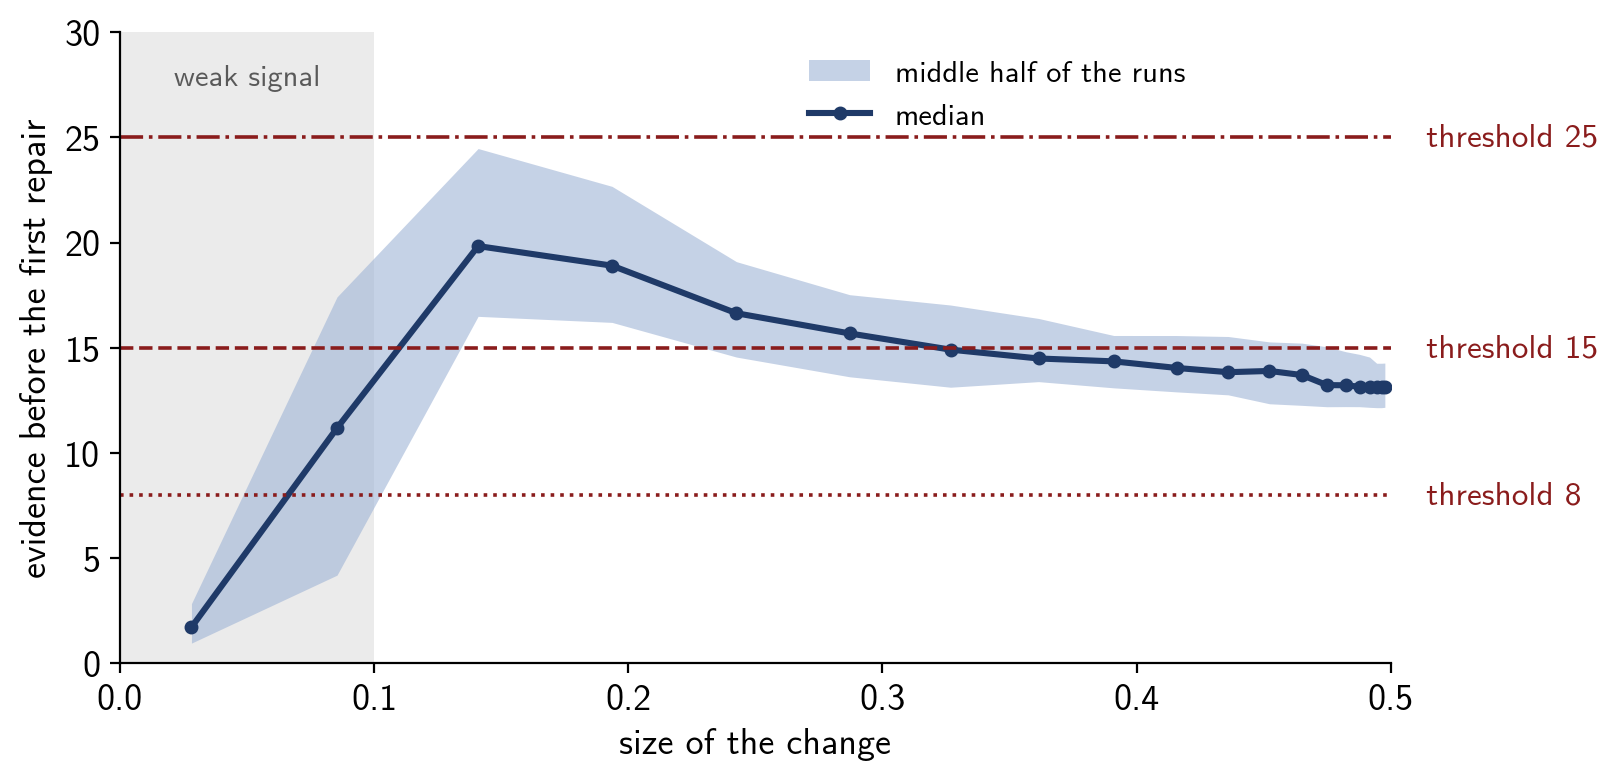
\includegraphics[width=\textwidth]{Fig_slide_spre.png}
    \end{column}\hfill
    \begin{column}{0.37\textwidth}
      \begin{itemize}
        \item Above the weak-signal zone, the median lies between \textbf{$13.1$ and $19.8$}:
              the transition the paper sees between $15$ and $25$, \alert{and leaves
              unexplained}.
        \item It \textbf{decreases} as the drift grows: at $\lambda = 15$ the detector wins
              $81\%$, then only $18\%$. That is the paradox.
      \end{itemize}
    \end{column}
  \end{columns}
  \note{So we measured S pre on every run. The dark line is the median by drift size, the band
    holds the middle half of the runs, and the red lines are thresholds. Above the weak-signal
    zone, the median sits between thirteen and twenty. A threshold below that level is reached
    before the repair in most runs; a threshold above it rarely is. That is exactly the
    transition the paper observes between fifteen and twenty-five, and leaves to future work.
    Now look at the shape. After the medium drifts, S pre decreases as the drift gets stronger,
    because the first replacement comes sooner. At a fixed threshold of fifteen, the detector
    wins eighty-one percent of the races on medium drifts, and only eighteen percent on the
    strongest ones. The paradox is this decreasing evidence, read against a fixed threshold. At
    the far left, the drift is too weak to accumulate anything: that is a different regime.}
\end{frame}

\begin{frame}{Stronger drifts leave no more evidence}
  \begin{columns}[c,onlytextwidth]
    \begin{column}{0.48\textwidth}
      \centering
      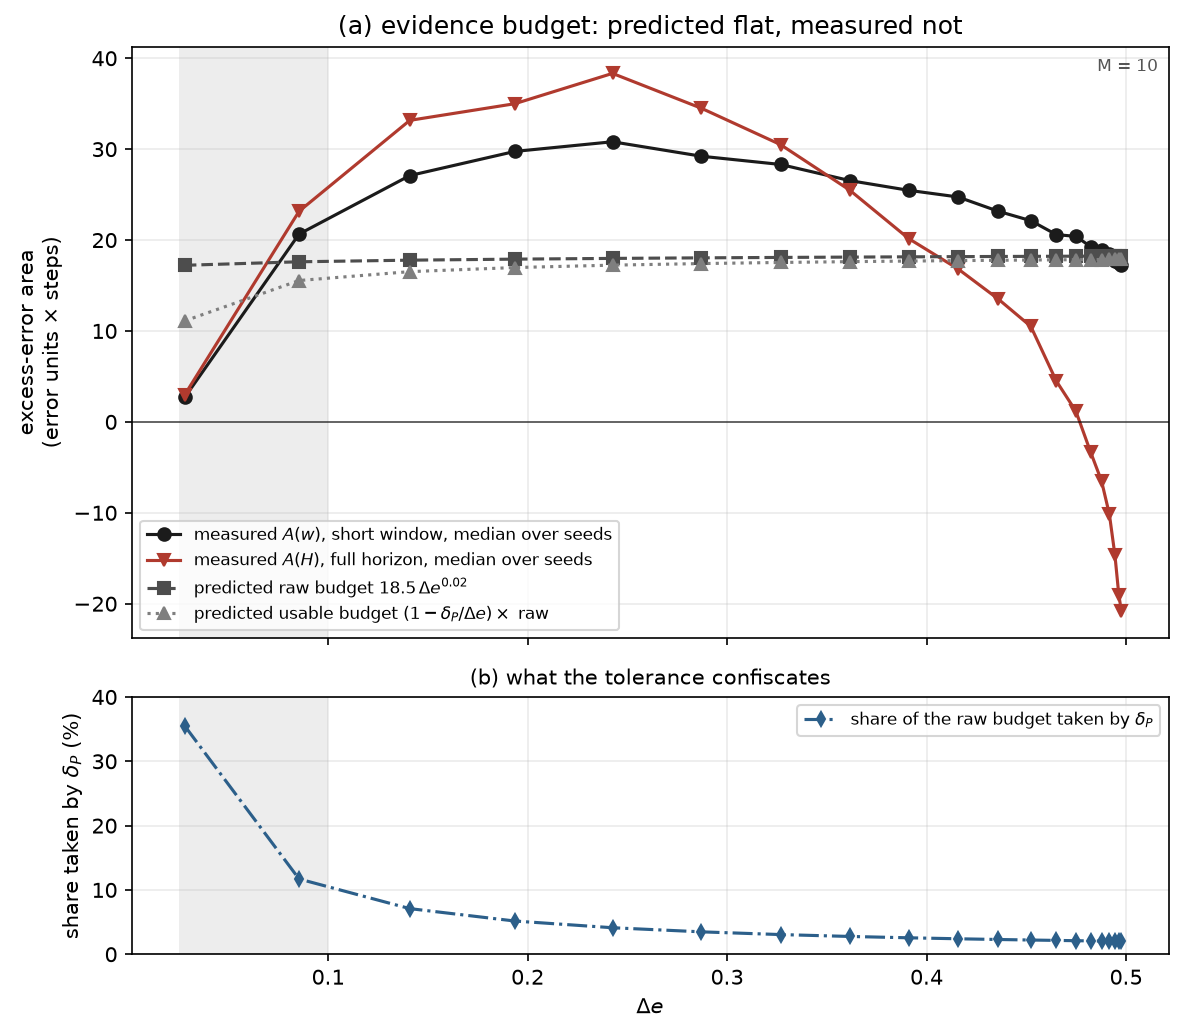
\includegraphics[height=0.66\textheight]{Fig_QC_budget_utilisable_full.png}
    \end{column}\hfill
    \begin{column}{0.46\textwidth}
      \begin{itemize}
        \item The paper's picture: an excess error $\Delta e$ over a window $\tau_{\mathrm{ARF}}$,
              so the area stays almost constant.
        \item Measured over the transition, the area varies by a factor of $1.8$ while the
              drift size varies by $5.8$: \alert{the compensation is real}.
        \item But the paper's rectangle misestimates it by up to $43\%$, and over the whole
              horizon the area turns negative at large drifts: the new task is easier.
      \end{itemize}
    \end{column}
  \end{columns}
  \note{Why doesn't a violent drift leave more evidence than a gentle one? The paper's picture
    is a rectangle: an excess error of height delta e, during a window equal to the repair
    time. Since the repair time shrinks like one over delta e, the area stays almost constant.
    We measured the area directly. Over the transition, it varies by a factor of less than two,
    while the drift size varies by almost six: the compensation is real. But the rectangle
    itself is wrong. It misestimates the area by up to forty-three percent, because the first
    replacement is not the width of the transient. And over the whole horizon, at large drifts,
    the area even becomes negative: after the change the task is easier than before, and the
    error settles below its old level. The evidence exists, it is roughly constant, but the
    paper's derivation of it does not hold.}
\end{frame}

\begin{frame}{Detecting is not winning}
  \begin{center}
    \begin{tabular}{@{}cccc@{}}
      \toprule
      threshold $\lambda$ & alarm fires & detector arrives first & false alarms, no drift \\
      \midrule
      $8$  & $95.3\%$ & $\mathbf{91.0\%}$ & $4.15\%$ \\
      $15$ & $92.9\%$ & $\mathbf{36.3\%}$ & $0.15\%$ \\
      $20$ & $66.2\%$ & $8.1\%$           & $0.00\%$ \\
      $25$ & $38.9\%$ & $2.5\%$           & $0.00\%$ \\
      \bottomrule
    \end{tabular}\\[0.3em]
    {\scriptsize\color{gray} $2\,000$ runs with drift and $2\,000$ without, over $2\,000$ steps}
  \end{center}
  \begin{itemize}
    \item At $\lambda = 15$ the alarm almost always fires, but mostly \emph{after} the repair.
    \item At $\lambda = 8$ the detector wins at an ordinary false-alarm cost: the paper's
          ``no threshold escapes'' does not hold on this bench.
    \item \textcolor{gray}{Not tested: the heteroscedastic streams where the paper places its
          false-alarm tension.}
  \end{itemize}
  \note{One practical consequence. Detecting a drift and winning the race are two different
    things. At threshold fifteen, the alarm fires on ninety-three percent of drifts, which
    looks excellent, but it arrives before the repair in only thirty-six percent of them.
    Most of these alarms come after the forest has already changed. At threshold eight, the
    detector wins ninety-one percent of the races, and it costs about four percent of false
    alarms over two thousand steps where nothing happens, which is an ordinary calibration
    level. So on this bench, one threshold does escape the blind spot, and the paper's claim
    that no threshold escapes has to be restricted. We did not test the financial streams
    with clustered volatility, where the paper places the false-alarm problem.}
\end{frame}

% =====================================================================
\section{Conclusion}
% =====================================================================

\begin{frame}{What changes in the paper}
  \small
  \begin{tabular}{@{}p{0.34\textwidth}p{0.43\textwidth}l@{}}
    \toprule
    The paper & Our result & \\
    \midrule
    races the repair against a constant & race identified, bounded, decided run by run & \textbf{made exact} \\
    independent trees, bias asserted & direction proven, cannot reverse & \textbf{proven} \\
    error back to normal at the first replacement & it comes back later; the rectangle fails & \textbf{corrected} \\
    first replacement as the repair date & earliest date, fires without drift & \textbf{qualified} \\
    transition between $15$ and $25$, unexplained & set by the evidence before the repair & \textbf{explained} \\
    no threshold escapes & $\lambda = 8$ does, on this bench & \textbf{restricted} \\
    \bottomrule
  \end{tabular}
  \vspace{0.6em}
  \begin{center}
    \alert{The phenomenon survives. What changes is its mechanism and its reach.}
  \end{center}
  \note{To sum up what our work changes in the paper. The race, which compared a random time
    with a constant, is made exact: identified, bounded, and decided run by run. The bias of
    the independence assumption was asserted; it is now proven, with its direction. The idea
    that the error is back to normal at the first replacement is corrected. The first
    replacement as a repair date is qualified: it is the earliest date and it fires without
    drift. The transition threshold, which the paper left unexplained, is explained by the
    evidence before the repair. And the claim that no threshold escapes is restricted to the
    settings the paper actually tested. The phenomenon survives all of this. What changes is
    its mechanism, and its reach.}
\end{frame}

\begin{frame}{An open question, and what we did not do}
  \begin{columns}[T,onlytextwidth]
    \begin{column}{0.50\textwidth}
      \begin{exampleblock}{Open: a reference for adaptation}
        Every indicator on the detector's side reads the \emph{error}, which mixes what the
        forest relearned with how hard the new task is. On analytic probes, the forest can
        relearn the changed region and lose a rare one, unseen by the error.
      \end{exampleblock}
    \end{column}\hfill
    \begin{column}{0.46\textwidth}
      \begin{block}{Not done}
        \small
        \begin{itemize}
          \item one forest size, one homoscedastic bench
          \item decision rule fixed during the analysis
          \item the independence bias has a sign, not a size
        \end{itemize}
      \end{block}
    \end{column}
  \end{columns}
  \note{We leave one question open. Every measure available to the detector reads the error,
    and the error mixes two things: what the forest has relearned, and how hard the new task
    is. Using analytic probes, points whose true label we know, we saw that the forest can
    relearn the region that changed while losing a rare region elsewhere, and the error does
    not see that loss. So what would a true reference for adaptation be? We do not have the
    answer. And to be honest about the limits: we studied one forest size on one simple
    bench, our decision rule was fixed during the analysis rather than before it, and we can
    give the sign of the independence bias but not its size.}
\end{frame}

\begin{frame}{Take-away}
  \begin{center}
    \small\alert{The blind spot is a budget of evidence, accumulated before the repair, set
    against a threshold.}
  \end{center}
  \vspace{-0.5em}
  \begin{center}\carte[0.71]{0}\end{center}
  \note{Back to the map. The blind spot is real, and it survives every correction. But it is
    not a race between two clocks. It is the evidence the forest lets through before its first
    repair, set against a fixed threshold. That single quantity explains when the detector
    wins, why the transition sits where it does, and why stronger drifts are missed more
    often. Thank you for your attention; we are happy to take your questions.}
\end{frame}

% =====================================================================
\appendix
\section*{Backup}
% =====================================================================

\begin{frame}{Backup --- Fréchet bounds}
  For integer-valued clocks with marginal CDFs $F_A$ and $F_D$, and \emph{any} coupling,
  \begin{align*}
    P_{\mathrm{miss}} &\ge \max\Big(0,\ \sup_{s} \big[F_A(s)-F_D(s)\big]\Big),\\
    P_{\mathrm{miss}} &\le \min\Big(1,\ \inf_{s} \big[F_A(s) + 1 - F_D(s+1)\big]\Big).
  \end{align*}
  \begin{itemize}
    \item Lower: Fréchet on $\{\tau_{\mathrm{ARF}} \le s < \tau_{\mathrm{det}}\} \subseteq \mathrm{Miss}$.
    \item Upper: $\mathrm{Miss} \subseteq \{\tau_{\mathrm{ARF}} \le s\} \cup \{\tau_{\mathrm{det}} > s+1\}$, then Boole.
    \item Toy case, both clocks uniform on $\{1,2\}$: the bounds $0$ and $0.5$ are both attained.
  \end{itemize}
\end{frame}

\begin{frame}{Backup --- Lindley's closed form and the certificate}
  With $X_t = e_t - \hat p_0 - \delta_P$ and $A(k,j) = \sum_{t=k+1}^{j} (e_t - \hat p_0)$,
  \[
    S_j = \max_{0 \le k \le j} \sum_{t=k+1}^{j} X_t,
    \qquad
    S_{\max}(H) = \max_{0 \le k \le j \le H} \big[A(k,j) - (j-k)\,\delta_P\big].
  \]
  \begin{itemize}
    \item Certificate: the alarm fires by $H$ iff some sub-window carries
          $A(k,j) \ge \lambda + (j-k)\,\delta_P$. The full window alone is only sufficient.
    \item Race identity: the same maximum, taken up to the first replacement, is $S_{\mathrm{pre}}$.
  \end{itemize}
\end{frame}

\begin{frame}{Backup --- Association protocol}
  \begin{itemize}
    \item Every coefficient is computed \textbf{within a drift size} ($100$ seeds), on the $18$
          sizes with $\Delta e \ge 0.10$: pooling measures the drift size, not the link.
    \item Kendall's $\tau_b$: reads on pairs, corrects for ties. Censored durations ranked last,
          licit because the horizon is common to all runs.
    \item Pearson undefined on censored values; Spearman handles their ties implicitly.
    \item Percentile bootstrap over seeds, $2\,000$ resamples; discernible if the interval
          excludes zero. Fixed during the analysis, not before: stated in the report.
    \item Complete cases instead of ranking censored runs last: no coefficient moves by more
          than $0.0403$.
  \end{itemize}
\end{frame}

\begin{frame}{Backup --- The drift-free control}
  \begin{center}
    \begin{tabular}{@{}lr@{}}
      \toprule
      On $2\,000$ runs with no change point & \\
      \midrule
      runs where at least one tree is replaced & $2\,000/2\,000$ \\
      first replacement, median & $95$ steps \\
      distinct trees renewed, median & $9/10$ \\
      forest entirely renewed & $28.7\%$ \\
      \midrule
      first replacement at the weakest drift, median & $118$ steps \\
      \bottomrule
    \end{tabular}
  \end{center}
\end{frame}

\end{document}
"
%
% Tracabilite : chaque chiffre vient du rapport ; controle par
%   verif_chiffres_tex.py ../../05_presentation/soutenance_20min.tex
% Figures : figures_slides.py --latex, figures_soutenance.py,
%   matrice_correlations.py, analyse_QCD.py (budget).
% =====================================================================

\documentclass[aspectratio=169,11pt]{beamer}

\usetheme{Madrid}
% Rouge de CentraleSupelec, pris dans le logo officiel (#B00739) ; logo
% CentraleSupelec / Universite Paris-Saclay sur la page de titre.
\definecolor{csRouge}{HTML}{B00739}
\usecolortheme[named=csRouge]{structure}
\setbeamercolor{alerted text}{fg=csRouge}
\setbeamersize{text margin left=1cm, text margin right=1cm}
\setbeamertemplate{navigation symbols}{}
\usepackage[english,french]{babel}
\usepackage{amsmath,amssymb}
\usepackage{graphicx}
\usepackage{booktabs}
\usepackage{tikz}
% soutenance_schemas.tex
% =====================================================================
% Schemas TikZ de `soutenance_20min.tex` : la carte des idees et le schema
% de l'identite de course.
%
% Fichier separe pour la meme raison que `point_encadrant_schemas.tex` :
% `verif_chiffres_tex.py` ramasserait les coordonnees TikZ comme des mesures.
% AUCUN chiffre de mesure ici ; les schemas sont stylises, sans donnees.
% =====================================================================

\usetikzlibrary{positioning, arrows.meta, calc}

\definecolor{mTheorie}{RGB}{31,58,104}
\definecolor{mDate}{RGB}{138,28,28}
\definecolor{mPreuve}{RGB}{38,92,58}
\definecolor{mEteint}{gray}{0.74}

% ---------------------------------------------------------------------
% \carte[hauteur]{k} : la carte des idees.
%   k = 0 : tout est actif (ouverture et conclusion)
%   k = 1, 2, 3 : seule la partie k est en couleur, le reste est grise
%   hauteur : fraction de \textheight (0.80 par defaut)
% Les fleches en pointille relient les parties ; elles sont commentees a
% l'oral plutot qu'etiquetees, faute de place entre les colonnes.
% ---------------------------------------------------------------------
\newcommand{\carte}[2][0.80]{%
  \colorlet{cUn}{mEteint}\colorlet{cDeux}{mEteint}\colorlet{cTrois}{mEteint}%
  \colorlet{tUn}{mEteint}\colorlet{tDeux}{mEteint}\colorlet{tTrois}{mEteint}%
  \ifnum#2=0 \colorlet{cUn}{mTheorie}\colorlet{cDeux}{mDate}\colorlet{cTrois}{mPreuve}%
    \colorlet{tUn}{black}\colorlet{tDeux}{black}\colorlet{tTrois}{black}\fi
  \ifnum#2=1 \colorlet{cUn}{mTheorie}\colorlet{tUn}{black}\fi
  \ifnum#2=2 \colorlet{cDeux}{mDate}\colorlet{tDeux}{black}\fi
  \ifnum#2=3 \colorlet{cTrois}{mPreuve}\colorlet{tTrois}{black}\fi
  \resizebox{!}{#1\textheight}{%
  \begin{tikzpicture}[
      font=\normalsize, align=center,
      boite/.style={draw, line width=1pt, rounded corners=3pt, inner sep=4pt,
                    text width=4.3cm, minimum height=1.05cm},
      un/.style={boite, draw=cUn, text=tUn},
      deux/.style={boite, draw=cDeux, text=tDeux},
      trois/.style={boite, draw=cTrois, text=tTrois},
      tete/.style={font=\bfseries\normalsize, text width=4.8cm},
      fl/.style={-{Stealth[length=2.4mm]}, line width=0.9pt},
      lien/.style={-{Stealth[length=2.4mm]}, line width=0.9pt, dashed},
    ]
    \node[boite, draw=black, fill=black!4, text width=12cm, minimum height=0.8cm] (P) at (5.6,0.15)
      {\textbf{The paper:} the stronger the drift, the faster the repair, the fewer the alarms};

    \node[tete, text=cUn]    (H1) at (0,-1.05)    {I.\ The race, formally};
    \node[tete, text=cDeux]  (H2) at (5.6,-1.05)  {II.\ The repair date};
    \node[tete, text=cTrois] (H3) at (11.2,-1.05) {III.\ Evidence vs threshold};
    \draw[fl, black!55] (P.south) -- ++(0,-0.25) -| (H1.north);
    \draw[fl, black!55] (P.south) -- (H2.north);
    \draw[fl, black!55] (P.south) -- ++(0,-0.25) -| (H3.north);

    \node[un] (A1) at (0,-2.1)  {The miss is well defined, its probability identified};
    \node[un] (A2) at (0,-3.45) {The blind spot holds whatever the dependence};
    \node[un] (B1) at (0,-4.8)  {Independent trees overstate the speed of repair};

    \node[deux] (C1) at (5.6,-2.1)  {The first replacement is the earliest date};
    \node[deux] (E1) at (5.6,-3.45) {It fires as fast when nothing changes};
    \node[deux] (D1) at (5.6,-4.8)  {When it fires, half the evidence is there};
    \node[deux] (D2) at (5.6,-6.15) {Indicators form two groups, weakly linked};

    \node[trois] (C2) at (11.2,-2.1)  {The alarm is a function of the error path};
    \node[trois] (K)  at (11.2,-3.45) {Detector first \emph{iff} it reaches $\lambda$ before the repair};
    \node[trois] (S)  at (11.2,-4.8)  {That evidence sets the transition and the paradox};
    \node[trois] (T)  at (11.2,-6.15) {Detecting is not winning};

    \node[boite, draw=black!55, text=black!80, dashed, text width=7cm, minimum height=0.8cm] (O) at (5.6,-7.45)
      {\textbf{Open:} a reference for adaptation itself};

    \draw[fl, cUn]    (A1) -- (A2);
    \draw[fl, cDeux]  (C1) -- (E1);
    \draw[fl, cDeux]  (E1) -- (D1);
    \draw[fl, cDeux]  (D1) -- (D2);
    \draw[fl, cTrois] (C2) -- (K);
    \draw[fl, cTrois] (K) -- (S);
    \draw[fl, cTrois] (S) -- (T);
    \draw[lien, black!55] (B1.east) -- (D1.west);
    \draw[lien, black!55] (D1.east) -- (S.west);
    \draw[lien, black!55] (D2.south) -- (O.north);
  \end{tikzpicture}}%
}

% ---------------------------------------------------------------------
% \schemaidentite : la pile S_t, le premier remplacement, deux seuils.
% Stylise, sans donnees.
% ---------------------------------------------------------------------
\newcommand{\schemaidentite}{%
  \begin{tikzpicture}[x=1cm, y=1cm, font=\small]
    \draw[-{Stealth}, line width=0.7pt] (0,0) -- (7.2,0);
    \node[below left] at (7.2,-0.05) {time};
    \draw[-{Stealth}, line width=0.7pt] (0,0) -- (0,3.7);
    \node[rotate=90, above] at (-0.05,1.85) {detector statistic $S_t$};
    \draw[line width=1.4pt, mTheorie]
      (0,0) .. controls (0.8,0.6) and (1.6,1.9) .. (2.4,2.25)
            .. controls (3.0,2.5) and (3.4,2.55) .. (3.9,2.4)
            .. controls (4.8,2.0) and (5.8,1.0) .. (7.0,0.3);
    \draw[dashed, mDate, line width=1pt] (2.8,0) -- (2.8,3.4);
    \node[above, text=mDate] at (2.8,3.4) {first replacement};
    \fill[mTheorie] (2.8,2.38) circle (2.3pt);
    \node[above left, text=mTheorie] at (2.75,2.4) {$S_{\mathrm{pre}}$};
    \draw[mPreuve, line width=1pt] (0,1.5) -- (7.0,1.5);
    \node[above left, text=mPreuve] at (7.0,1.5) {low $\lambda$: reached before};
    \draw[mDate, line width=1pt, dash dot] (0,3.0) -- (7.0,3.0);
    \node[above left, text=mDate] at (7.0,3.0) {high $\lambda$: not reached};
  \end{tikzpicture}%
}

\titlegraphic{
\includegraphics[height=1.7cm]{Logo_CS_Paris_Saclay.png}}
\ifdefined\NOTESSEULES\setbeameroption{show only notes}\fi
\graphicspath{{../04_experimentations/resultats_R2/resultats/figures/slides_latex/}{../04_experimentations/resultats_R2/resultats/figures/}}

\setbeamerfont{author}{size=\small}
\setbeamerfont{institute}{size=\scriptsize}

\title[The Blind Spot Paradox]{The Blind Spot Paradox}
\subtitle{Formalizing the race and measuring the adaptation}
\author[Boyer, Gouillou, Fonvielle, Petit-Tichanné]{Alexandre Boyer \and Melaine Gouillou \and Salomé Fonvielle \and Ulysse Petit-Tichanné}
\institute[CS]{Research Track, Topic 39, CentraleSupélec. Supervisor: Raphaël Minato}
\date{16 September 2026}

\begin{document}

\maketitle
\note{Bonjour à tous. Notre sujet est le paradoxe du point aveugle : un modèle qui se
  répare lui-même peut détruire la preuve même dont son propre moniteur a besoin. Dans
  les vingt prochaines minutes, nous présenterons ce que nous avons formalisé, ce que
  nous avons mesuré, et la lecture unique qui relie les deux.}

% =====================================================================
\section{The problem}
% =====================================================================

\begin{frame}{Concept drift: the rule changes, the data does not}
  \vspace{-0.6em}
  \[
    \underbrace{P(X)}_{\text{the data}}\ \text{unchanged}
    \qquad\qquad
    \underbrace{P(Y \mid X)}_{\text{the rule}}\ \text{changes}
  \]
  \vspace{-0.9em}
  \begin{center}
    
\includegraphics[height=0.50\textheight]{Fig_slide_drift.png}
  \end{center}
  \begin{center}
    A model trained before the change is now \alert{wrong on the shaded band}.
  \end{center}
  \note{Un classifieur apprend une règle à partir de données. Dans un flux, cette règle peut
    changer alors que les entrées gardent exactement la même distribution. C'est le concept
    drift : P de X ne bouge pas, P de Y sachant X bouge. C'est la situation normale d'un
    signal financier, où les mêmes entrées cessent de vouloir dire la même chose. Sur le banc
    que nous utilisons, des points du plan sont séparés par une droite. Au changement, la
    droite se déplace. Chaque point de la bande grisée change d'étiquette, si bien qu'un
    modèle entraîné avant le changement continue de prédire avec assurance, et se trompe
    désormais sur cette bande. La largeur de la bande est la taille du drift, notée delta e.}
\end{frame}

\begin{frame}{Two defences that run at the same time}
  \begin{columns}[T,onlytextwidth]
    \begin{column}{0.49\textwidth}
      \centering
      \textbf{The model repairs itself}\\[0.3em]
      
\includegraphics[width=\textwidth]{Fig_slide_foret.png}\\[0.2em]
      \small Adaptive Random Forest: ten trees, each replaced when its own error rises.
    \end{column}\hfill
    \begin{column}{0.49\textwidth}
      \centering
      \textbf{A monitor raises the alarm}\\[0.3em]
      
\includegraphics[width=\textwidth]{Fig_slide_watchdog.png}\\[0.2em]
      \small Each error adds to a statistic $S_t$; the alarm fires when it crosses $\lambda$.
    \end{column}
  \end{columns}
  \note{Deux défenses sont déployées ensemble. La première vit à l'intérieur du modèle. La
    forêt aléatoire adaptative est faite de dix arbres de décision qui votent. Chaque arbre
    surveille sa propre erreur avec un petit détecteur, et quand cette erreur monte, l'arbre
    est remplacé par un neuf. La forêt se répare localement, sans demander à personne. La
    seconde défense est à l'extérieur. Un détecteur cumulatif, un test de Page-Hinkley,
    surveille l'erreur de toute la forêt. Chaque erreur pousse une statistique vers le haut
    de presque un, chaque bonne réponse la tire un peu vers le bas, jamais sous zéro. Quand
    la statistique franchit un seuil lambda, l'alarme part, et cette alarme est la seule
    chose qu'un opérateur humain voit.}
\end{frame}

\begin{frame}{The paradox, and what the reviewers asked}
  \begin{columns}[c,onlytextwidth]
    \begin{column}{0.50\textwidth}
      \centering
      
\includegraphics[width=\textwidth]{Fig_slide_mecanisme.png}\\
      {\scriptsize\color{gray} schematic}
    \end{column}\hfill
    \begin{column}{0.46\textwidth}
      \begin{block}{The paper's claim}
        The stronger the drift, the faster the repair, and the \alert{fewer} alarms.
      \end{block}
      \begin{alertblock}{Two corrections requested}
        \begin{enumerate}
          \item It races a random repair time against a \emph{constant}, and assumes the
                trees independent.
          \item It dates the repair at the \emph{first} tree replaced, without showing
                that this date means anything.
        \end{enumerate}
      \end{alertblock}
    \end{column}
  \end{columns}
  \note{Quand les deux défenses tournent ensemble, il se passe quelque chose d'inattendu. Le
    drift commence, les erreurs s'accumulent dans le détecteur, mais la forêt remplace des
    arbres, les erreurs s'arrêtent, et le tas se vide avant d'atteindre le seuil. L'article
    que nous étudions appelle cela le paradoxe du point aveugle : plus le drift est fort,
    plus la forêt se répare vite, et moins l'opérateur reçoit d'alarmes. L'article a été
    relu, et deux corrections ont été demandées. D'abord, il compare un temps de réparation
    aléatoire à un temps de détection constant, et il suppose les dix arbres indépendants
    sans le prouver. Ensuite, il date la réparation au moment où le premier arbre est
    remplacé, sans montrer que ce moment a quoi que ce soit à voir avec la disparition de
    l'erreur. C'est de ces deux corrections que part notre travail.}
\end{frame}

\begin{frame}{Our reading, in one map}
  \begin{center}
    \small\alert{The blind spot is not a race between two clocks,
    but a budget of evidence set against a threshold.}
  \end{center}
  \vspace{-0.5em}
  \begin{center}
    \carte[0.71]{0}
  \end{center}
  \note{Voici tout l'exposé sur une seule carte. En haut, l'affirmation de l'article. La
    première colonne formalise la course : nous définissons proprement le point aveugle,
    nous calculons sa probabilité, et nous montrons que supposer les arbres indépendants
    rend l'article optimiste sur la réparation. La deuxième colonne demande ce que la date
    de réparation mesure réellement : c'est la date la plus précoce possible, elle se
    déclenche même quand rien ne change, et quand elle se déclenche l'essentiel de la preuve
    est déjà là. La troisième colonne relie les deux : le détecteur gagne exactement quand sa
    preuve atteint le seuil avant la réparation, et cette preuve explique à la fois la
    transition et le paradoxe. Les flèches en pointillés sont les liens entre colonnes, et
    la boîte du bas est la question que nous laissons ouverte. Notre lecture en une phrase :
    le point aveugle n'est pas une course entre deux horloges, c'est un budget de preuve
    face à un seuil.}
\end{frame}

% =====================================================================
\section{I. The race}
% =====================================================================

\begin{frame}{Part I --- The race, formally}
  \begin{center}\carte{1}\end{center}
  \note{Commençons par la théorie : comment énoncer la course sans tricher.}
\end{frame}

\begin{frame}{The race is well posed, and its probability identified}
  \begin{columns}[T,onlytextwidth]
    \begin{column}{0.46\textwidth}
      \begin{block}{One definition, no ad hoc rule}
        \[
          \mathrm{Miss} := \{\tau_{\mathrm{ARF}} < \tau_{\mathrm{det}}\}
        \]
        \vspace{-0.6em}
        {\small strict inequality; the alarm may never come}
        \begin{itemize}
          \item a tie goes to the detector
          \item a silent repair, with no alarm ever, \alert{is} a miss
          \item if neither acts, it is not
        \end{itemize}
      \end{block}
    \end{column}\hfill
    \begin{column}{0.50\textwidth}
      \begin{exampleblock}{What the campaign allows}
        The forest always replaces a tree within the horizon, so no run is left
        undecided: $P_{\mathrm{miss}}$ is \textbf{identified}.\\[0.3em]
        \centering
        {\small all $20$ drift sizes pooled:}\\[0.1em]
        \begin{tabular}{@{}lccc@{}}
          $\lambda$ & $8$ & $25$ & $50$ \\
          $P_{\mathrm{miss}}$ & $0.0905$ & $0.9715$ & $1.0000$
        \end{tabular}
      \end{exampleblock}
      \begin{alertblock}{Without any dependence assumption}
        From the marginal laws alone, the blind spot at the weakest drift
        ($\Delta e = 0.028$, observed $1.00$) is at least $0.91$ at $\lambda = 8$.
      \end{alertblock}
    \end{column}
  \end{columns}
  \vspace{0.3em}
  {\scriptsize\color{gray} $\tau_{\mathrm{ARF}}$: first tree replaced \quad
   $\tau_{\mathrm{det}}$: first alarm \quad $\Delta e$: drift size, the jump in error}
  \note{L'article dit qu'il y a point aveugle quand la forêt se répare avant l'alarme, mais
    il écarte discrètement les runs où l'alarme ne vient jamais. Ce sont exactement les runs
    où le détecteur échoue le plus. Nous définissons donc l'événement sur la course
    complète, avec une seule définition et aucune règle supplémentaire. Une égalité compte
    pour le détecteur, parce que l'opérateur est prévenu au bon moment. Une réparation
    silencieuse, où l'alarme ne vient jamais, est un raté, et même le plus pur. Un run où
    aucun des deux mécanismes n'agit n'est pas un raté, parce qu'il n'y avait rien à
    effacer. Vient ensuite le problème de l'horizon fini : certains runs pourraient rester
    indécis. Sur notre campagne ils ne le sont pas, parce que la forêt agit toujours avant
    l'horizon, donc la probabilité de raté est identifiée exactement : neuf pour cent au
    seuil huit, quatre-vingt-dix-sept à vingt-cinq, cent à cinquante. Et avec les bornes de
    Fréchet, qui n'utilisent que les deux lois marginales et ne supposent rien sur le
    couplage des horloges, le point aveugle au drift le plus faible est déjà forcé au-dessus
    de quatre-vingt-dix pour cent.}
\end{frame}

\begin{frame}{Trees share a stream: the paper is optimistic}
  \begin{enumerate}
    \item \textbf{Given the stream}, what separates two trees is their own random draws:
          the trees are independent \emph{conditionally}.
    \item \textbf{Hence the covariance of two trees is a variance}, never negative: sharing
          a stream can only make them fail together --- the forest is \emph{slower} than
          the independence formula says.
    \item \textbf{More precisely}, averaging over streams, convexity gives the bound:
          \[
            P(\tau_{\mathrm{ARF}} \le s) \;\le\; 1 - \big(1 - F(s)\big)^M
          \]
    \item \textbf{Conclusion}: \alert{the independence formula overstates the speed of
          the repair}, hence the blind spot; the paper's critical ensemble size becomes a
          conservative ceiling, and its verdict does not change.
  \end{enumerate}
  \note{Le second raccourci est l'indépendance. Les dix arbres apprennent sur le même flux,
    ils ne peuvent donc pas être indépendants. Mais la question est : à quel niveau. Une
    fois le flux fixé, ce qui distingue un arbre d'un autre n'est plus que son aléa propre,
    les poids aléatoires du bagging en ligne. À ce niveau, sachant le flux, les arbres sont
    indépendants. C'est une propriété de l'algorithme, et tout le reste en découle. D'abord
    le sens : le seul canal entre deux arbres est le flux qu'ils partagent, et un flux
    partagé ne peut que les faire échouer ensemble, puisque leur covariance se réduit à une
    variance. La vraie forêt se répare donc plus lentement que ne le dit la formule
    d'indépendance. Ensuite la taille : en moyennant sur les flux, l'inégalité de Jensen
    donne une majoration, la probabilité que la forêt se soit déjà réparée est au plus ce
    que la formule d'indépendance prédit. L'article fait donc paraître la forêt plus rapide
    qu'elle n'est, et surestime le point aveugle. Sa taille critique d'ensemble n'est pas
    fausse, elle devient un plafond conservateur, et le verdict de l'article lui-même ne
    change pas.}
\end{frame}

% =====================================================================
\section{II. The repair date}
% =====================================================================

\begin{frame}{Part II --- What the repair date measures}
  \begin{center}\carte{2}\end{center}
  \note{Passons à la seconde correction : la date que l'article utilise pour la réparation.}
\end{frame}

\begin{frame}{How we measured}
  \begin{columns}[T,onlytextwidth]
    \begin{column}{0.48\textwidth}
      \begin{block}{The campaign}
        \begin{itemize}
          \item the paper's bench, rerun: $20$ drift sizes $\times$ $100$ seeds,
                $2\,000$ steps after the change
          \item $2\,000$ more runs with no change at all
          \item only the error and the replacement events are recorded; every threshold is
                replayed offline
        \end{itemize}
      \end{block}
    \end{column}\hfill
    \begin{column}{0.48\textwidth}
      \begin{block}{Reading an association}
        \begin{itemize}
          \item always \alert{within one drift size}: pooling measures the drift size, not
                the link
          \item Kendall's rank correlation, with bootstrap intervals over the seeds
          \item steps added after seeing the data are flagged as exploratory
        \end{itemize}
      \end{block}
    \end{column}
  \end{columns}
  \note{Un mot sur la façon dont nous avons mesuré, sans les détails d'implémentation. Nous
    avons rejoué le banc de l'article sur vingt tailles de drift, avec cent graines chacune,
    et nous observons deux mille pas après le changement. Nous avons ajouté deux mille runs
    où rien ne change du tout, comme témoin. La simulation n'enregistre que deux choses :
    l'erreur à chaque pas et les instants où des arbres sont remplacés. Tout le reste, y
    compris le détecteur à n'importe quel seuil, est recalculé hors ligne, si bien qu'une
    campagne en remplace plusieurs. Quand nous corrélons deux grandeurs, nous le faisons
    toujours à taille de drift fixée. La taille du drift déplace tous les indicateurs à la
    fois, donc une corrélation mélangeant les tailles mesure surtout la taille elle-même.
    Nous utilisons la corrélation de rang de Kendall avec des intervalles bootstrap, et nous
    signalons les étapes ajoutées après avoir regardé les données.}
\end{frame}

\begin{frame}{The first replacement is the earliest possible date}
  \begin{center}
    
\includegraphics[width=0.90\textwidth]{Fig_slide_deux_horloges.png}
  \end{center}
  \vspace{-0.3em}
  \begin{itemize}
    \item On every run, the first replacement comes before any other quota of renewed
          trees. Three quarters of the forest are renewed \textbf{$6.0$ to $14.3$ times later}.
    \item \alert{With no drift at all}, the first replacement comes after $95$ steps in
          median, against $118$ on the weakest drift.
    \item On weak drifts it comes \emph{later}: $346$ steps at $\Delta e = 0.085$. With no drift
          but the same error level, it also waits $268$: the error level delays it, not the change.
  \end{itemize}
  \note{L'article date la réparation au premier arbre remplacé. Par construction, c'est la
    plus précoce de toutes les dates possibles : le moment où trois arbres, ou la moitié, ou
    les trois quarts de la forêt sont remplacés vient toujours après, sur chaque run. La
    seule question est : combien de temps après. Sur ce drift moyen, le premier arbre tombe
    après quatre-vingt-six observations, et les trois quarts de la forêt après plus de douze
    cents. Sur la grille, les trois quarts de la forêt sont renouvelés six à quatorze fois
    plus tard que le premier arbre. Et il y a un fait plus inquiétant. Sur les deux mille
    runs sans aucun changement, la forêt remplace quand même son premier arbre, après
    quatre-vingt-quinze pas en médiane. Sur le drift réel le plus faible, il lui en faut cent
    dix-huit. Donc à faible drift, cette date ne distingue pas un vrai changement du bruit.
    Pire, sur un drift un peu plus fort elle vient plus tard, après trois cent quarante-six
    pas. Nous avons vérifié pourquoi avec un second témoin sans drift, où l'on élève seulement
    le niveau d'erreur en retournant des étiquettes. Au même niveau d'erreur, le premier
    remplacement attend aussi environ deux cent soixante-dix pas. Le détecteur interne de
    chaque arbre coupe moins souvent quand l'erreur est plus bruitée, donc sur les drifts
    faibles cette date mesure le niveau d'erreur, pas le changement.}
\end{frame}

\begin{frame}{When the first tree goes, most of the evidence is already there}
  \begin{columns}[T,onlytextwidth]
    \begin{column}{0.36\textwidth}
      \begin{block}{Evidence at the first replacement}
        \centering
        {\Large $49\%$ to $76\%$}\\[0.2em]
        \small of the detector's final peak, on the $18$ drift sizes studied
      \end{block}
    \end{column}\hfill
    \begin{column}{0.60\textwidth}
      \begin{block}{Does the date track anything, within a drift size?}
        \small
        \begin{tabular}{@{}lcc@{}}
          \toprule
          compared with & median link & sizes \\
          \midrule
          detector peak & $0.21$ & $15/18$ \\
          excess error, whole horizon & none & $0/18$ \\
          excess error, transition only & $0.23$ & $13/18$ \\
          \bottomrule
        \end{tabular}
      \end{block}
    \end{column}
  \end{columns}
  \vspace{0.8em}
  \begin{center}
    \small The null over the whole horizon is mostly noise: \alert{half} of that area's
    variance comes from the estimated baseline, multiplied by the horizon.
  \end{center}
  \note{Le premier remplacement est-il au moins la fin du transitoire ? Non. Quand le premier
    arbre est remplacé, le détecteur détient déjà entre la moitié et les trois quarts de
    toute la preuve qu'il accumulera jamais. Le remplacement est au milieu de l'histoire, pas
    à sa fin. Nous avons ensuite demandé si cette date suit quelque chose, toujours à taille
    de drift fixée. Avec le pic du détecteur, il y a un lien faible mais réel, visible sur
    quinze tailles de drift sur dix-huit. Avec l'erreur excédentaire sur tout l'horizon, il
    n'y a aucun lien. Mais nous avons compris pourquoi : cette aire additionne deux mille
    pas, donc toute erreur sur le socle est multipliée par deux mille, et la moitié de sa
    variance n'est que ce bruit. Si l'on ne garde que la transition, le lien revient, faible
    mais réel, sur treize tailles sur dix-huit. Cette dernière étape est exploratoire.}
\end{frame}

\begin{frame}{Unexpected: pooling manufactures agreement}
  \begin{center}
    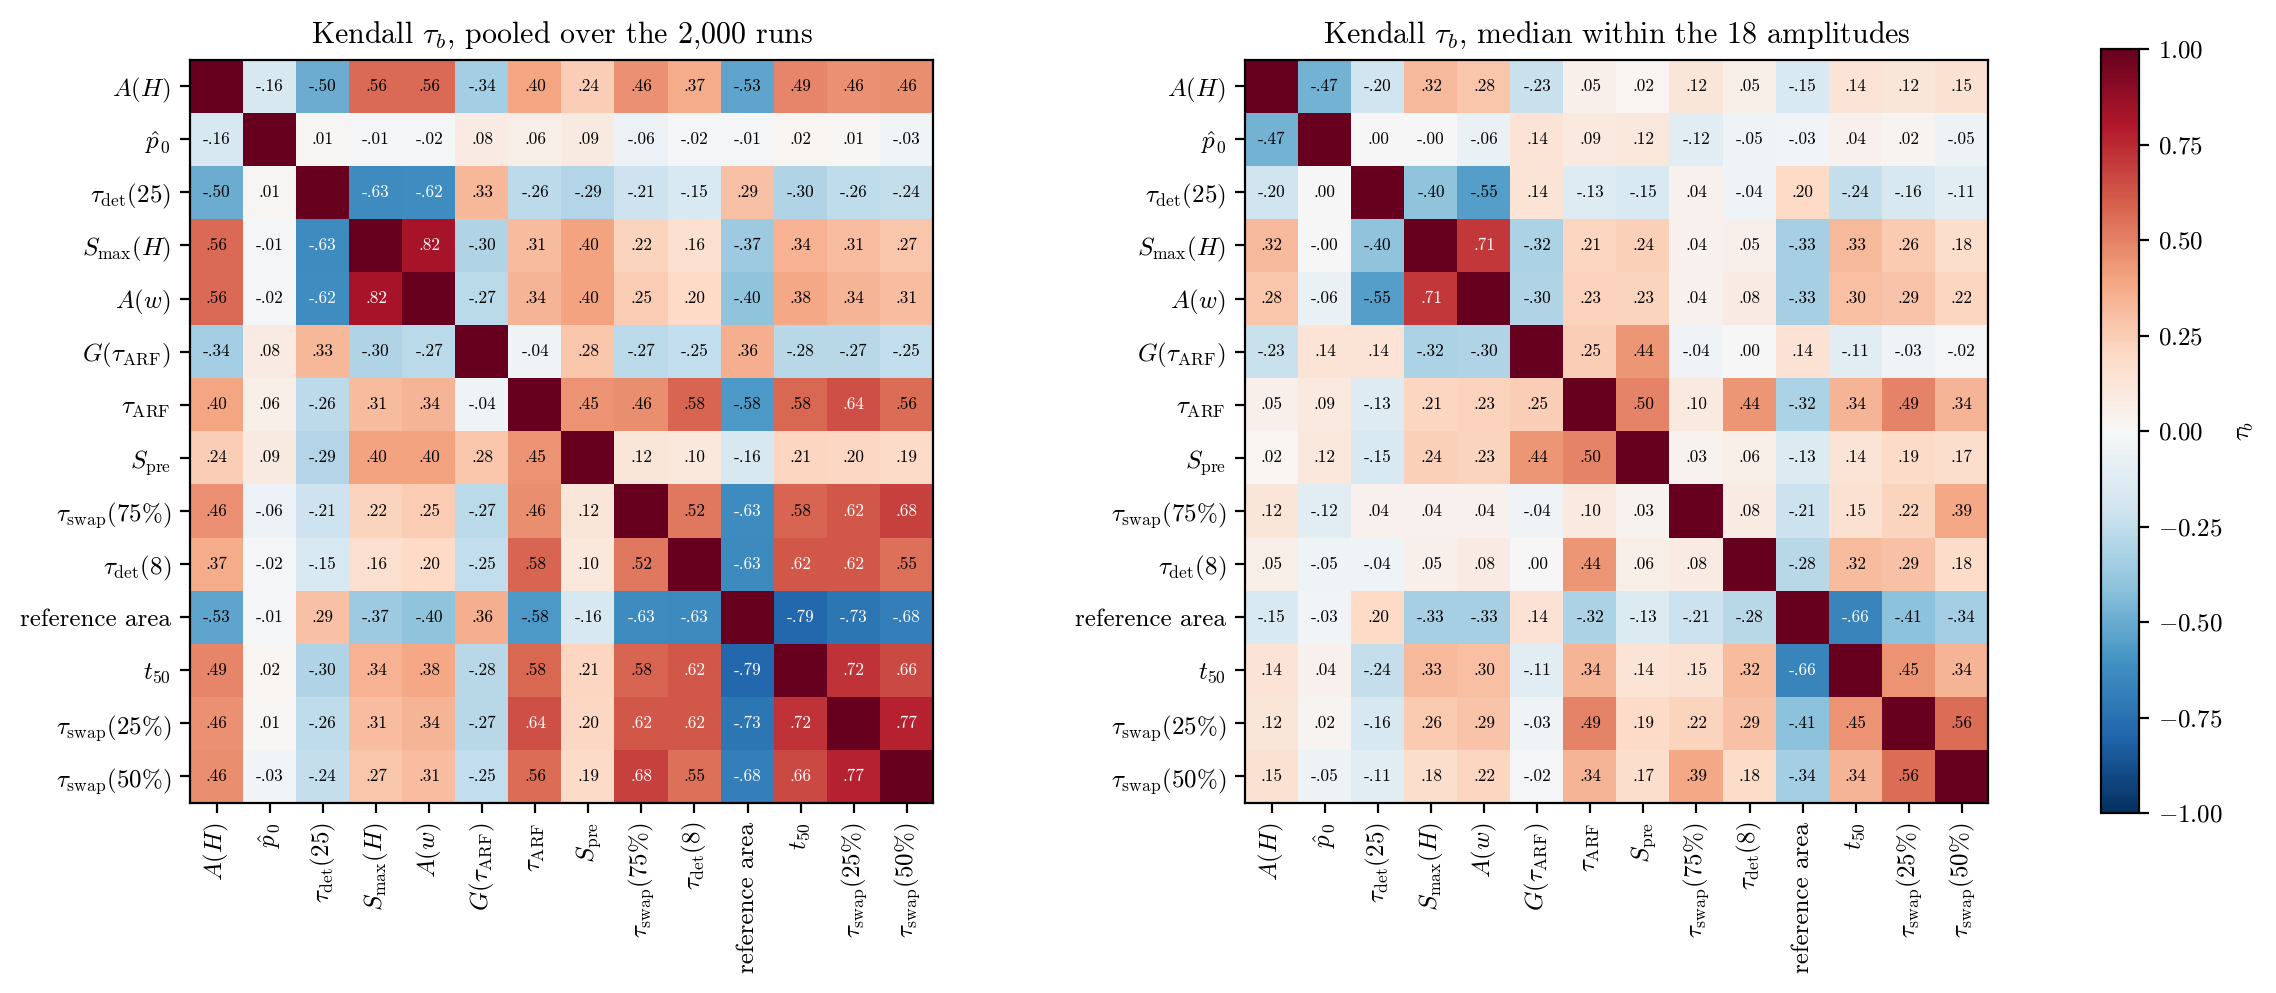
\includegraphics[width=0.86\textwidth]{Fig_QD_matrice_correlations_full.png}
  \end{center}
  \vspace{-0.5em}
  \small
  \begin{columns}[T,onlytextwidth]
    \begin{column}{0.32\textwidth}
      \textbf{Left, pooled:} almost everything agrees, because the drift size moves every
      indicator.
    \end{column}\hfill
    \begin{column}{0.32\textwidth}
      \textbf{Right, within a size:} two groups remain, \emph{evidence} ($0.71$) and
      \emph{repair}, weakly joined.
    \end{column}\hfill
    \begin{column}{0.32\textwidth}
      Best date against the analytic reference: \alert{3 trees replaced}, $0.45$, ahead of
      the first tree, $0.34$.
    \end{column}
  \end{columns}
  \note{Pour voir tous les indicateurs d'un coup, nous en avons croisé quatorze. Le panneau
    de gauche mélange tous les runs : presque tout est fortement corrélé avec tout. C'est une
    illusion, le paradoxe de Simpson : la taille du drift déplace chaque indicateur, donc le
    mélange fabrique de l'accord. Le panneau de droite calcule les mêmes corrélations à
    l'intérieur de chaque taille de drift. L'essentiel de l'accord disparaît, et deux groupes
    subsistent. Un groupe mesure la preuve et les dégâts : le pic du détecteur et l'erreur
    excédentaire sur la transition s'accordent fortement. L'autre groupe mesure la
    réparation. Entre les deux groupes, les liens restent faibles. Nous avons aussi comparé
    les dates de remplacement à une référence analytique, la précision de la forêt sur la
    région dont l'étiquette a changé. La date à laquelle trois arbres sont remplacés la suit
    mieux que le premier arbre. Cette matrice est exploratoire.}
\end{frame}

% =====================================================================
\section{III. Evidence vs threshold}
% =====================================================================

\begin{frame}{Part III --- Evidence against the threshold}
  \begin{center}\carte{3}\end{center}
  \note{La troisième partie relie les deux premières.}
\end{frame}

\begin{frame}{The race is decided before the repair}
  \begin{columns}[c,onlytextwidth]
    \begin{column}{0.52\textwidth}
      \centering
      \resizebox{\linewidth}{!}{\schemaidentite}\\
      {\scriptsize\color{gray} schematic}
    \end{column}\hfill
    \begin{column}{0.44\textwidth}
      A time counts observations; $\lambda$ counts \emph{excess errors}. Comparing them
      needs a rate that does not exist.
      \begin{block}{Race identity, on every run}
        \vspace{-0.4em}
        \[
          \tau_{\mathrm{det}} < \tau_{\mathrm{ARF}}
          \iff S_{\mathrm{pre}} \ge \lambda
        \]
        \vspace{-0.9em}
        \[
          S_{\mathrm{pre}} = \max_{t < \tau_{\mathrm{ARF}}} S_t
        \]
      \end{block}
      \vspace{-0.3em}
      {\scriptsize\color{gray} $S_{\mathrm{pre}}$: the highest the detector's evidence gets
       before the forest repairs itself\par}
      \vspace{0.3em}
      \small No rate, no averaging, no assumption on the trees. Checked on $2\,000$ runs out
      of $2\,000$ at three thresholds.
    \end{column}
  \end{columns}
  \note{Voici l'étape clé. Un temps de réparation compte des observations. Un seuil compte
    des erreurs excédentaires. Ils ne sont pas dans la même unité, et l'article fait le pont
    avec un taux moyen d'erreurs par pas. Ce taux n'existe pas : il chute à mesure que la
    forêt se répare, et le détecteur oublie sa preuve chaque fois qu'il touche zéro.
    L'énoncé exact est bien plus simple. Regardez la statistique du détecteur jusqu'au
    premier remplacement, et prenez son point le plus haut : nous l'appelons S pré. Le
    détecteur arrive premier si et seulement si S pré atteint le seuil. Avec un seuil bas, il
    est atteint avant la réparation ; avec un seuil haut, il ne l'est pas. C'est exact sur
    chaque run, ça ne demande ni taux, ni moyenne, ni hypothèse sur les arbres, et nous
    l'avons vérifié sur les deux mille runs.}
\end{frame}

\begin{frame}{The evidence before the repair sets the transition}
  \begin{columns}[c,onlytextwidth]
    \begin{column}{0.60\textwidth}
      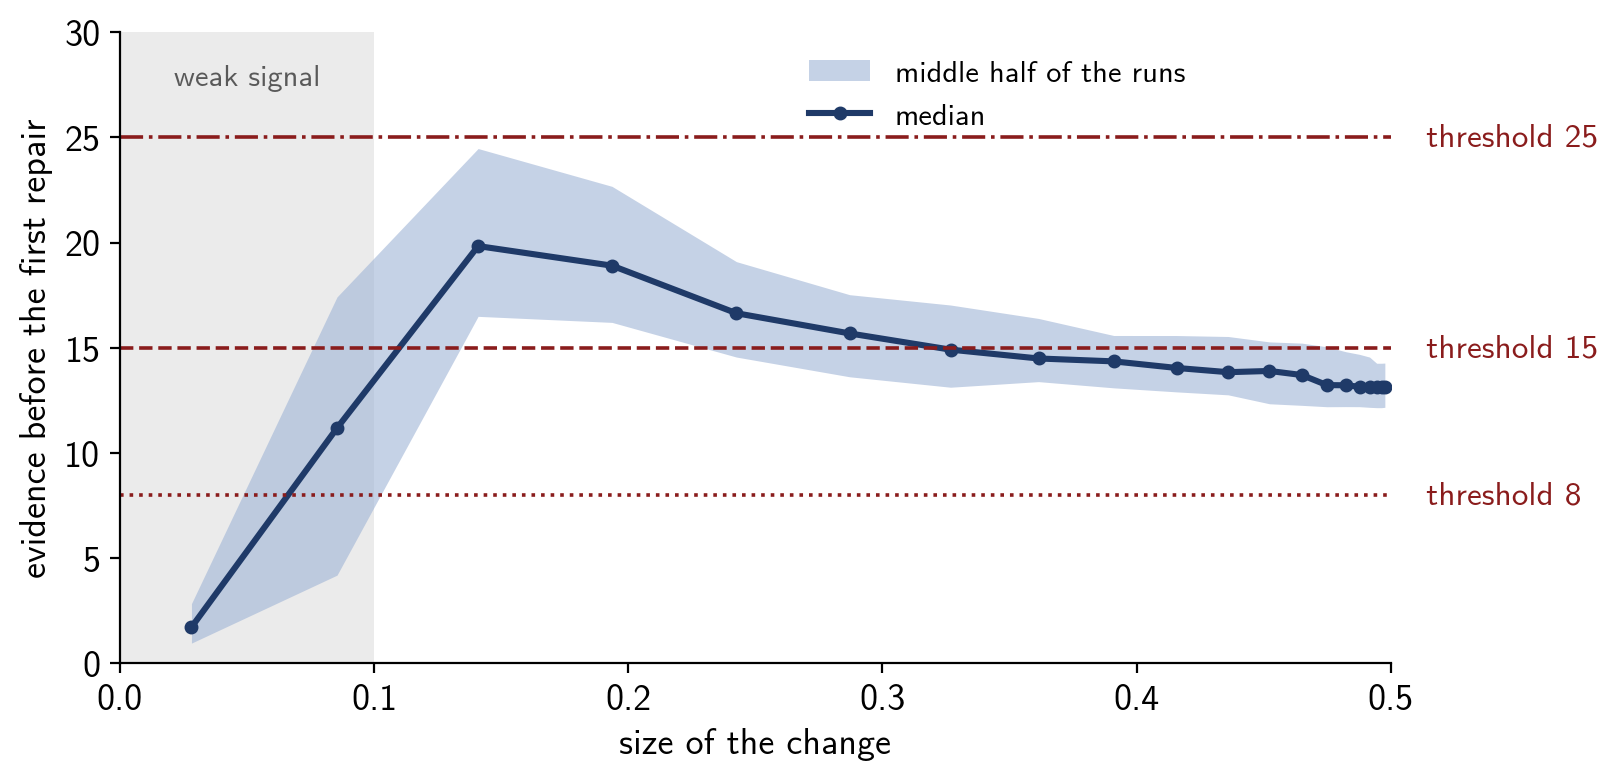
\includegraphics[width=\textwidth]{Fig_slide_spre.png}
    \end{column}\hfill
    \begin{column}{0.37\textwidth}
      \begin{itemize}
        \item Above the weak-signal zone, the median lies between \textbf{$13.1$ and $19.8$}:
              the transition the paper sees between $15$ and $25$, \alert{and leaves
              unexplained}.
        \item It \textbf{decreases} as the drift grows: at $\lambda = 15$ the detector wins
              $81\%$, then only $18\%$. That is the paradox.
      \end{itemize}
    \end{column}
  \end{columns}
  \note{Nous avons donc mesuré S pré sur chaque run. La ligne sombre est la médiane par
    taille de drift, la bande contient la moitié centrale des runs, et les lignes rouges sont
    des seuils. Au-dessus de la zone de signal faible, la médiane se situe entre treize et
    vingt. Un seuil sous ce niveau est atteint avant la réparation dans la plupart des runs ;
    un seuil au-dessus l'est rarement. C'est exactement la transition que l'article observe
    entre quinze et vingt-cinq, et qu'il laisse aux travaux futurs. Regardez maintenant la
    forme. Après les drifts moyens, S pré décroît quand le drift se renforce, parce que le
    premier remplacement vient plus tôt. À seuil fixé à quinze, le détecteur gagne
    quatre-vingt-un pour cent des courses sur les drifts moyens, et seulement dix-huit pour
    cent sur les plus forts. Le paradoxe, c'est cette preuve décroissante, lue face à un
    seuil fixe. Tout à gauche, le drift est trop faible pour accumuler quoi que ce soit :
    c'est un autre régime.}
\end{frame}

\begin{frame}{Stronger drifts leave no more evidence}
  \begin{columns}[c,onlytextwidth]
    \begin{column}{0.48\textwidth}
      \centering
      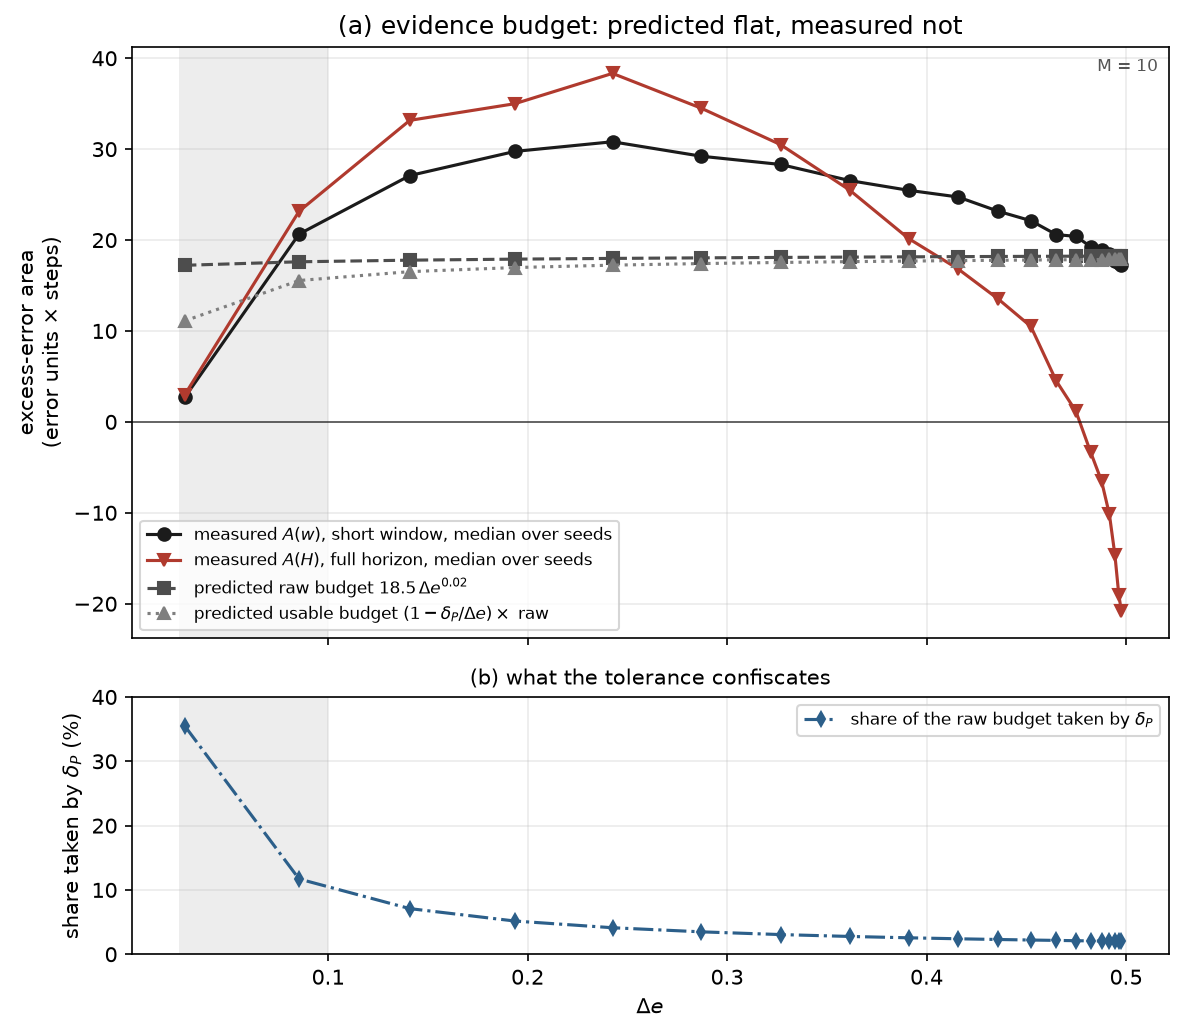
\includegraphics[height=0.66\textheight]{Fig_QC_budget_utilisable_full.png}
    \end{column}\hfill
    \begin{column}{0.46\textwidth}
      \begin{itemize}
        \item The paper's picture: an excess error $\Delta e$ over a window $\tau_{\mathrm{ARF}}$,
              so the area stays almost constant.
        \item Measured over the transition, the area varies by a factor of $1.8$ while the
              drift size varies by $5.8$: \alert{the compensation is real}.
        \item But the paper's rectangle misestimates it by up to $43\%$, and over the whole
              horizon the area turns negative at large drifts: the new task is easier.
      \end{itemize}
    \end{column}
  \end{columns}
  \note{Pourquoi un drift violent ne laisse-t-il pas plus de preuve qu'un drift doux ?
    L'image de l'article est un rectangle : une erreur excédentaire de hauteur delta e,
    pendant une fenêtre égale au temps de réparation. Comme le temps de réparation décroît
    comme un sur delta e, l'aire reste presque constante. Nous avons mesuré l'aire
    directement. Sur la transition, elle varie d'un facteur inférieur à deux, alors que la
    taille du drift varie de presque six : la compensation est réelle. Mais le rectangle
    lui-même est faux. Il se trompe sur l'aire jusqu'à quarante-trois pour cent, parce que le
    premier remplacement n'est pas la largeur du transitoire. Et sur tout l'horizon, aux
    grands drifts, l'aire devient même négative : après le changement, la tâche est plus
    facile qu'avant, et l'erreur se stabilise sous son ancien niveau. La preuve existe, elle
    est à peu près constante, mais la dérivation qu'en fait l'article ne tient pas.}
\end{frame}

\begin{frame}{Detecting is not winning}
  \begin{center}
    \begin{tabular}{@{}cccc@{}}
      \toprule
      threshold $\lambda$ & alarm fires & detector arrives first & false alarms, no drift \\
      \midrule
      $8$  & $95.3\%$ & $\mathbf{91.0\%}$ & $4.15\%$ \\
      $15$ & $92.9\%$ & $\mathbf{36.3\%}$ & $0.15\%$ \\
      $20$ & $66.2\%$ & $8.1\%$           & $0.00\%$ \\
      $25$ & $38.9\%$ & $2.5\%$           & $0.00\%$ \\
      \bottomrule
    \end{tabular}\\[0.3em]
    {\scriptsize\color{gray} $2\,000$ runs with drift and $2\,000$ without, over $2\,000$ steps}
  \end{center}
  \begin{itemize}
    \item At $\lambda = 15$ the alarm almost always fires, but mostly \emph{after} the repair.
    \item At $\lambda = 8$ the detector wins $91\%$ of races for $4.15\%$ of drift-free runs
          with a false alarm: the paper's ``no threshold escapes'' does not hold on this bench.
    \item \textcolor{gray}{Not tested: the heteroscedastic streams where the paper places its
          false-alarm tension.}
  \end{itemize}
  \note{Une conséquence pratique. Détecter un drift et gagner la course sont deux choses
    différentes. Au seuil quinze, l'alarme part sur quatre-vingt-treize pour cent des
    drifts, ce qui paraît excellent, mais elle arrive avant la réparation dans seulement
    trente-six pour cent d'entre eux. La plupart de ces alarmes viennent après que la forêt a
    déjà changé. Au seuil huit, le détecteur gagne quatre-vingt-onze pour cent des courses,
    et environ quatre pour cent des runs où rien ne se passe lèvent une fausse alarme en deux
    mille pas. Au seuil douze, il gagne encore soixante-dix-neuf pour cent des courses, pour
    un demi pour cent de fausses alarmes. Donc sur ce banc, les seuils bas échappent bel et
    bien au point aveugle, et l'affirmation de l'article qu'aucun seuil n'y échappe doit
    être restreinte. Nous n'avons pas testé les flux financiers à volatilité groupée, où
    l'article situe le problème des fausses alarmes.}
\end{frame}

% =====================================================================
\section{Conclusion}
% =====================================================================

\begin{frame}{What changes in the paper}
  \small
  \begin{tabular}{@{}p{0.34\textwidth}p{0.43\textwidth}l@{}}
    \toprule
    The paper & Our result & \\
    \midrule
    races the repair against a constant & race identified, bounded, decided run by run & \textbf{made exact} \\
    independent trees, bias asserted & direction proven, cannot reverse & \textbf{proven} \\
    error back to normal at the first replacement & it comes back later; the rectangle fails & \textbf{corrected} \\
    first replacement as the repair date & earliest date, fires without drift & \textbf{qualified} \\
    transition between $15$ and $25$, unexplained & set by the evidence before the repair & \textbf{explained} \\
    no threshold escapes & $\lambda = 8$ and $12$ do, on this bench & \textbf{restricted} \\
    \bottomrule
  \end{tabular}
  \vspace{0.6em}
  \begin{center}
    \alert{The phenomenon survives. What changes is its mechanism and its reach.}
  \end{center}
  \note{Pour résumer ce que notre travail change dans l'article. La course, qui comparait un
    temps aléatoire à une constante, est rendue exacte : identifiée, bornée, et décidée run
    par run. Le biais de l'hypothèse d'indépendance était affirmé ; il est maintenant
    prouvé, avec son sens. L'idée que l'erreur est revenue à la normale au premier
    remplacement est corrigée. Le premier remplacement comme date de réparation est
    qualifié : c'est la date la plus précoce et elle se déclenche sans drift. Le seuil de
    transition, que l'article laissait inexpliqué, est expliqué par la preuve avant la
    réparation. Et l'affirmation qu'aucun seuil n'échappe est restreinte aux réglages que
    l'article a réellement testés. Le phénomène survit à tout cela. Ce qui change, c'est son
    mécanisme, et sa portée.}
\end{frame}

\begin{frame}{An open question, and what we did not do}
  \begin{columns}[T,onlytextwidth]
    \begin{column}{0.50\textwidth}
      \begin{exampleblock}{Open: a reference for adaptation}
        Every indicator on the detector's side reads the \emph{error}, which mixes what the
        forest relearned with how hard the new task is. On analytic probes, the forest can
        relearn the changed region and lose a rare one, unseen by the error.
      \end{exampleblock}
    \end{column}\hfill
    \begin{column}{0.46\textwidth}
      \begin{block}{Not done}
        \small
        \begin{itemize}
          \item one forest size, one homoscedastic bench
          \item decision rule fixed during the analysis
          \item the independence bias has a sign, not a size
        \end{itemize}
      \end{block}
    \end{column}
  \end{columns}
  \note{Nous laissons une question ouverte. Toute mesure disponible pour le détecteur lit
    l'erreur, et l'erreur mélange deux choses : ce que la forêt a réappris, et la difficulté
    de la nouvelle tâche. Avec des sondes analytiques, des points dont nous connaissons la
    vraie étiquette, nous avons vu que la forêt peut réapprendre la région qui a changé tout
    en perdant une région rare ailleurs, et l'erreur ne voit pas cette perte. Alors quelle
    serait une vraie référence pour l'adaptation ? Nous n'avons pas la réponse. Et pour être
    honnêtes sur les limites : nous avons étudié une seule taille de forêt sur un seul banc
    simple, notre règle de décision a été fixée pendant l'analyse plutôt qu'avant, et nous
    pouvons donner le signe du biais d'indépendance mais pas sa taille.}
\end{frame}

\begin{frame}{Take-away}
  \begin{center}
    \small\alert{The blind spot is a budget of evidence, accumulated before the repair, set
    against a threshold.}
  \end{center}
  \vspace{-0.5em}
  \begin{center}\carte[0.71]{0}\end{center}
  \note{Retour à la carte. Le point aveugle est réel, et il survit à toutes les corrections.
    Mais ce n'est pas une course entre deux horloges. C'est la preuve que la forêt laisse
    passer avant sa première réparation, face à un seuil fixe. Cette seule grandeur explique
    quand le détecteur gagne, pourquoi la transition est là où elle est, et pourquoi les
    drifts plus forts sont ratés plus souvent. Merci de votre attention ; nous sommes à votre
    disposition pour vos questions.}
\end{frame}

% =====================================================================
\appendix
\section*{Backup}
% =====================================================================

\begin{frame}{Backup --- The supervisor's additional questions}
  {\small Treated in a separate working document on the same campaign; not merged into the report.}
  \begin{itemize}
    \item \textbf{Shape of the error after the drift}: not exponential, and its half-recovery comes
          \emph{after} the median first replacement on $17$ of the $18$ readable drift sizes.
          The first replacement is early, again.
    \item \textbf{End of the horizon}: the error settles \emph{below} its pre-drift baseline at all
          $20$ drift sizes. The new task is easier.
    \item \textbf{Inside the forest} (pilot, $100$ runs): disagreement between trees halves when only
          $63$ to $66\%$ of them are renewed --- the surviving trees learn too. After a strong drift,
          new trees err far less than survivors.
    \item \textbf{A z-score of the error drop} measures the number of seeds, not the dynamics.
  \end{itemize}
  \vfill
  {\small\color{gray} Open, and worth continuing: a reference for adaptation, the size of the
  independence bias, heteroscedastic streams, tree-by-tree dynamics.}
\end{frame}

\begin{frame}{Backup --- Fréchet bounds}
  For integer-valued clocks with marginal CDFs $F_A$ and $F_D$, and \emph{any} coupling,
  \begin{align*}
    P_{\mathrm{miss}} &\ge \max\Big(0,\ \sup_{s} \big[F_A(s)-F_D(s)\big]\Big),\\
    P_{\mathrm{miss}} &\le \min\Big(1,\ \inf_{s} \big[F_A(s) + 1 - F_D(s+1)\big]\Big).
  \end{align*}
  \begin{itemize}
    \item Lower: Fréchet on $\{\tau_{\mathrm{ARF}} \le s < \tau_{\mathrm{det}}\} \subseteq \mathrm{Miss}$.
    \item Upper: $\mathrm{Miss} \subseteq \{\tau_{\mathrm{ARF}} \le s\} \cup \{\tau_{\mathrm{det}} > s+1\}$, then Boole.
    \item Toy case, both clocks uniform on $\{1,2\}$: the bounds $0$ and $0.5$ are both attained.
  \end{itemize}
\end{frame}

\begin{frame}{Backup --- Lindley's closed form and the certificate}
  With $X_t = e_t - \hat p_0 - \delta_P$ and $A(k,j) = \sum_{t=k+1}^{j} (e_t - \hat p_0)$,
  \[
    S_j = \max_{0 \le k \le j} \sum_{t=k+1}^{j} X_t,
    \qquad
    S_{\max}(H) = \max_{0 \le k \le j \le H} \big[A(k,j) - (j-k)\,\delta_P\big].
  \]
  \begin{itemize}
    \item Certificate: the alarm fires by $H$ iff some sub-window carries
          $A(k,j) \ge \lambda + (j-k)\,\delta_P$. The full window alone is only sufficient.
    \item Race identity: the same maximum, taken up to the first replacement, is $S_{\mathrm{pre}}$.
  \end{itemize}
\end{frame}

\begin{frame}{Backup --- Association protocol}
  \begin{itemize}
    \item Every coefficient is computed \textbf{within a drift size} ($100$ seeds), on the $18$
          sizes with $\Delta e \ge 0.10$: pooling measures the drift size, not the link.
    \item Kendall's $\tau_b$: reads on pairs, corrects for ties. Censored durations ranked last,
          licit because the horizon is common to all runs.
    \item Pearson undefined on censored values; Spearman handles their ties implicitly.
    \item Percentile bootstrap over seeds, $2\,000$ resamples; discernible if the interval
          excludes zero. Fixed during the analysis, not before: stated in the report.
    \item Complete cases instead of ranking censored runs last: no coefficient moves by more
          than $0.0403$.
  \end{itemize}
\end{frame}

\begin{frame}{Backup --- The drift-free control}
  \begin{center}
    \begin{tabular}{@{}lr@{}}
      \toprule
      On $2\,000$ runs with no change point & \\
      \midrule
      runs where at least one tree is replaced & $2\,000/2\,000$ \\
      first replacement, median & $95$ steps \\
      distinct trees renewed, median & $9/10$ \\
      forest entirely renewed & $28.7\%$ \\
      \midrule
      first replacement at the weakest drift, median & $118$ steps \\
      \bottomrule
    \end{tabular}
  \end{center}
\end{frame}

\begin{frame}{Backup --- Notation}
  \begin{center}
    \small
    \begin{tabular}{@{}ll@{}}
      \toprule
      $\Delta e$ & drift size: the jump in error a stale model suffers \\
      $\tau_{\mathrm{ARF}}$ & first tree replaced after the change \\
      $\tau_{\mathrm{swap}}(q)$ & first time a share $q$ of the trees has been replaced \\
      $\tau_{\mathrm{det}}$ & first alarm of the external detector, possibly never \\
      $S_t$, $\lambda$ & detector statistic and its threshold \\
      $S_{\mathrm{pre}}$ & highest $S_t$ reached before the first replacement \\
      $A(w)$, $A(H)$ & excess error over the transient window, over the whole horizon \\
      $G$ & share of the detector's final evidence already reached at $\tau_{\mathrm{ARF}}$ \\
      \bottomrule
    \end{tabular}
  \end{center}
\end{frame}

\end{document}
"
% soutenance_20min.tex
% =====================================================================
% Soutenance du 16/09/2026 : 20 minutes de presentation, 10 de questions.
%
% Trame : celle du rapport refondu. These : le point aveugle n'est pas une
% course entre deux horloges mais un budget de preuve contre un seuil. La
% carte des idees (soutenance_schemas.tex) ouvre le propos, revient en tete
% de chaque partie avec la partie en couleur, et le conclut.
%
% Consignes de l'encadrant : vue globale, concepts, resultats inattendus ;
% pas de details de preuve, de calcul ou d'implementation dans le corps.
% Les preuves et le protocole sont en slides de secours, apres la fin.
% Pas de renvoi aux numeros de questions du sujet (preference du groupe).
%
% Duree : les notes sont le texte parle, environ 2 600 mots, soit
% 20 minutes a 130 mots par minute.
%
% Style : Madrid, comme le pitch. Compilation : lualatex, deux passes.
% Notes seules : lualatex -jobname=soutenance_notes "\def\NOTESSEULES{}% soutenance_20min.tex
% =====================================================================
% Soutenance du 16/09/2026 : 20 minutes de presentation, 10 de questions.
%
% Trame : celle du rapport refondu. These : le point aveugle n'est pas une
% course entre deux horloges mais un budget de preuve contre un seuil. La
% carte des idees (soutenance_schemas.tex) ouvre le propos, revient en tete
% de chaque partie avec la partie en couleur, et le conclut.
%
% Consignes de l'encadrant : vue globale, concepts, resultats inattendus ;
% pas de details de preuve, de calcul ou d'implementation dans le corps.
% Les preuves et le protocole sont en slides de secours, apres la fin.
% Pas de renvoi aux numeros de questions du sujet (preference du groupe).
%
% Duree : les notes sont le texte parle, environ 2 600 mots, soit
% 20 minutes a 130 mots par minute.
%
% Style : Madrid, comme le pitch. Compilation : lualatex, deux passes.
% Notes seules : lualatex -jobname=soutenance_notes "\def\NOTESSEULES{}% soutenance_20min.tex
% =====================================================================
% Soutenance du 16/09/2026 : 20 minutes de presentation, 10 de questions.
%
% Trame : celle du rapport refondu. These : le point aveugle n'est pas une
% course entre deux horloges mais un budget de preuve contre un seuil. La
% carte des idees (soutenance_schemas.tex) ouvre le propos, revient en tete
% de chaque partie avec la partie en couleur, et le conclut.
%
% Consignes de l'encadrant : vue globale, concepts, resultats inattendus ;
% pas de details de preuve, de calcul ou d'implementation dans le corps.
% Les preuves et le protocole sont en slides de secours, apres la fin.
% Pas de renvoi aux numeros de questions du sujet (preference du groupe).
%
% Duree : les notes sont le texte parle, environ 2 600 mots, soit
% 20 minutes a 130 mots par minute.
%
% Style : Madrid, comme le pitch. Compilation : lualatex, deux passes.
% Notes seules : lualatex -jobname=soutenance_notes "\def\NOTESSEULES{}% soutenance_20min.tex
% =====================================================================
% Soutenance du 16/09/2026 : 20 minutes de presentation, 10 de questions.
%
% Trame : celle du rapport refondu. These : le point aveugle n'est pas une
% course entre deux horloges mais un budget de preuve contre un seuil. La
% carte des idees (soutenance_schemas.tex) ouvre le propos, revient en tete
% de chaque partie avec la partie en couleur, et le conclut.
%
% Consignes de l'encadrant : vue globale, concepts, resultats inattendus ;
% pas de details de preuve, de calcul ou d'implementation dans le corps.
% Les preuves et le protocole sont en slides de secours, apres la fin.
% Pas de renvoi aux numeros de questions du sujet (preference du groupe).
%
% Duree : les notes sont le texte parle, environ 2 600 mots, soit
% 20 minutes a 130 mots par minute.
%
% Style : Madrid, comme le pitch. Compilation : lualatex, deux passes.
% Notes seules : lualatex -jobname=soutenance_notes "\def\NOTESSEULES{}\input{soutenance_20min}"
%
% Tracabilite : chaque chiffre vient du rapport ; controle par
%   verif_chiffres_tex.py ../../05_presentation/soutenance_20min.tex
% Figures : figures_slides.py --latex, figures_soutenance.py,
%   matrice_correlations.py, analyse_QCD.py (budget).
% =====================================================================

\documentclass[aspectratio=169,11pt]{beamer}

\usetheme{Madrid}
% Rouge de CentraleSupelec, pris dans le logo officiel (#B00739) ; logo
% CentraleSupelec / Universite Paris-Saclay sur la page de titre.
\definecolor{csRouge}{HTML}{B00739}
\usecolortheme[named=csRouge]{structure}
\setbeamercolor{alerted text}{fg=csRouge}
\setbeamersize{text margin left=1cm, text margin right=1cm}
\setbeamertemplate{navigation symbols}{}
\usepackage[english]{babel}
\usepackage{amsmath,amssymb}
\usepackage{graphicx}
\usepackage{booktabs}
\usepackage{tikz}
\input{soutenance_schemas}
\titlegraphic{
\includegraphics[height=1.7cm]{Logo_CS_Paris_Saclay.png}}
\ifdefined\NOTESSEULES\setbeameroption{show only notes}\fi
\graphicspath{{../04_experimentations/resultats_R2/resultats/figures/slides_latex/}{../04_experimentations/resultats_R2/resultats/figures/}}

\setbeamerfont{author}{size=\small}
\setbeamerfont{institute}{size=\scriptsize}

\title[The Blind Spot Paradox]{The Blind Spot Paradox}
\subtitle{Formalizing the race and measuring the adaptation}
\author[Boyer, Gouillou, Fonvielle, Petit-Tichanné]{Alexandre Boyer \and Melaine Gouillou \and Salomé Fonvielle \and Ulysse Petit-Tichanné}
\institute[CS]{Research Track, Topic 39, CentraleSupélec. Supervisor: Raphaël Minato}
\date{16 September 2026}

\begin{document}

\maketitle
\note{Good afternoon. Our subject is the blind spot paradox: a model that repairs
  itself can destroy the very evidence its own monitor needs. In the next twenty
  minutes we will present what we formalized, what we measured, and the single
  reading that ties the two together.}

% =====================================================================
\section{The problem}
% =====================================================================

\begin{frame}{Concept drift: the rule changes, the data does not}
  \vspace{-0.6em}
  \[
    \underbrace{P(X)}_{\text{the data}}\ \text{unchanged}
    \qquad\qquad
    \underbrace{P(Y \mid X)}_{\text{the rule}}\ \text{changes}
  \]
  \vspace{-0.9em}
  \begin{center}
    
\includegraphics[height=0.50\textheight]{Fig_slide_drift.png}
  \end{center}
  \begin{center}
    A model trained before the change is now \alert{wrong on the shaded band}.
  \end{center}
  \note{A classifier learns a rule from data. In a data stream, that rule can change
    while the inputs keep exactly the same distribution. This is concept drift: P of X
    does not move, P of Y given X does. It is the normal situation for a financial
    signal, where the same inputs stop meaning the same thing. In the bench we use,
    points in the plane are separated by a line. At the change, the line moves. Every
    point in the shaded band switches label, so a model trained before the change keeps
    predicting confidently, and is now wrong on that band. The size of the band is the
    size of the drift, written delta e.}
\end{frame}

\begin{frame}{Two defences that run at the same time}
  \begin{columns}[T,onlytextwidth]
    \begin{column}{0.49\textwidth}
      \centering
      \textbf{The model repairs itself}\\[0.3em]
      
\includegraphics[width=\textwidth]{Fig_slide_foret.png}\\[0.2em]
      \small Adaptive Random Forest: ten trees, each replaced when its own error rises.
    \end{column}\hfill
    \begin{column}{0.49\textwidth}
      \centering
      \textbf{A monitor raises the alarm}\\[0.3em]
      
\includegraphics[width=\textwidth]{Fig_slide_watchdog.png}\\[0.2em]
      \small Each error adds to a statistic $S_t$; the alarm fires when it crosses $\lambda$.
    \end{column}
  \end{columns}
  \note{Two defences are deployed together. The first one lives inside the model. The
    Adaptive Random Forest is made of ten decision trees that vote. Each tree watches its
    own error with a small detector, and when that error rises, the tree is replaced by a
    fresh one. The forest repairs itself locally, without asking anyone. The second defence
    sits outside. A cumulative detector, a Page-Hinkley test, watches the error of the
    whole forest. Every error pushes a statistic up by almost one, every correct answer
    pulls it down a little, never below zero. When the statistic crosses a threshold
    lambda, the alarm fires, and that alarm is the only thing a human operator sees.}
\end{frame}

\begin{frame}{The paradox, and what the reviewers asked}
  \begin{columns}[c,onlytextwidth]
    \begin{column}{0.50\textwidth}
      \centering
      
\includegraphics[width=\textwidth]{Fig_slide_mecanisme.png}\\
      {\scriptsize\color{gray} schematic}
    \end{column}\hfill
    \begin{column}{0.46\textwidth}
      \begin{block}{The paper's claim}
        The stronger the drift, the faster the repair, and the \alert{fewer} alarms.
      \end{block}
      \begin{alertblock}{Two corrections requested}
        \begin{enumerate}
          \item It races a random repair time against a \emph{constant}, and assumes the
                trees independent.
          \item It dates the repair at the \emph{first} tree replaced, without showing
                that this date means anything.
        \end{enumerate}
      \end{alertblock}
    \end{column}
  \end{columns}
  \note{When both defences run together, something unexpected happens. The drift starts,
    errors pile up in the detector, but the forest replaces trees, the errors stop, and the
    pile drains before it reaches the threshold. The paper we study calls this the blind
    spot paradox: the stronger the drift, the faster the forest repairs itself, and the
    fewer alarms the operator gets. The paper was reviewed, and two corrections were
    requested. First, it compares a random repair time with a constant detection time, and
    it assumes the ten trees are independent without proving it. Second, it dates the repair
    at the moment the first tree is replaced, without showing that this moment has anything
    to do with the error disappearing. These two corrections are where our work starts.}
\end{frame}

\begin{frame}{Our reading, in one map}
  \begin{center}
    \small\alert{The blind spot is not a race between two clocks,
    but a budget of evidence set against a threshold.}
  \end{center}
  \vspace{-0.5em}
  \begin{center}
    \carte[0.71]{0}
  \end{center}
  \note{Here is the whole talk on one map. At the top, the claim of the paper. The first
    column formalizes the race: we define the blind spot properly, we compute its
    probability, and we show that assuming independent trees makes the paper optimistic
    about the repair. The second column asks what the repair date really measures: it is
    the earliest possible date, it fires even when nothing changes, and when it fires most
    of the evidence is already there. The third column ties both together: the detector wins
    exactly when its evidence reaches the threshold before the repair, and that evidence
    explains both the transition and the paradox. The dashed arrows are the links between
    columns, and the box at the bottom is the question we leave open. Our one-sentence
    reading: the blind spot is not a race between two clocks, it is a budget of evidence set
    against a threshold.}
\end{frame}

% =====================================================================
\section{I. The race}
% =====================================================================

\begin{frame}{Part I --- The race, formally}
  \begin{center}\carte{1}\end{center}
  \note{Let us start with the theory: how to state the race without cheating.}
\end{frame}

\begin{frame}{The race is well posed, and its probability identified}
  \begin{columns}[T,onlytextwidth]
    \begin{column}{0.46\textwidth}
      \begin{block}{One definition, no ad hoc rule}
        \[
          \mathrm{Miss} := \{\tau_{\mathrm{ARF}} < \tau_{\mathrm{det}}\}
        \]
        \vspace{-0.6em}
        {\small strict inequality; the alarm may never come}
        \begin{itemize}
          \item a tie goes to the detector
          \item a silent repair, with no alarm ever, \alert{is} a miss
          \item if neither acts, it is not
        \end{itemize}
      \end{block}
    \end{column}\hfill
    \begin{column}{0.50\textwidth}
      \begin{exampleblock}{What the campaign allows}
        The forest always replaces a tree within the horizon, so no run is left
        undecided: $P_{\mathrm{miss}}$ is \textbf{identified}.\\[0.3em]
        \centering
        \begin{tabular}{@{}lccc@{}}
          $\lambda$ & $8$ & $25$ & $50$ \\
          $P_{\mathrm{miss}}$ & $0.0905$ & $0.9715$ & $1.0000$
        \end{tabular}
      \end{exampleblock}
      \begin{alertblock}{Without any dependence assumption}
        From the marginal laws alone, the blind spot at the weakest drift is at least
        $0.91$ at $\lambda = 8$.
      \end{alertblock}
    \end{column}
  \end{columns}
  \note{The paper says there is a blind spot when the forest repairs before the alarm, but
    it quietly sets aside the runs where the alarm never comes. Those are exactly the runs
    where the detector fails most. So we define the event on the complete race, with one
    definition and no extra rule. A tie counts for the detector, because the operator is
    warned at the right moment. A silent repair, where the alarm never comes, is a miss, and
    in fact the purest one. A run where neither mechanism acts is not a miss, because there
    was nothing to erase. Then comes the problem of the finite horizon: some runs could be
    undecided. On our campaign they are not, because the forest always acts within the
    horizon, so the miss probability is identified exactly: nine percent at threshold eight,
    ninety-seven at twenty-five, one hundred at fifty. And with Fréchet bounds, which use the
    two marginal laws and assume nothing on how the clocks are coupled, the blind spot at the
    weakest drift is already forced above ninety percent.}
\end{frame}

\begin{frame}{Trees share a stream: the paper is optimistic}
  \begin{enumerate}
    \item \textbf{Given the stream}, what separates two trees is their own random draws:
          the trees are independent \emph{conditionally}.
    \item \textbf{Averaging over streams}, convexity gives the direction:
          \[
            P(\tau_{\mathrm{ARF}} \le s) \;\le\; 1 - \big(1 - F(s)\big)^M
          \]
          \alert{The independence formula overstates the speed of the repair.}
    \item \textbf{Consequence}: the paper's critical ensemble size becomes a conservative
          ceiling; its verdict does not change.
    \item \textbf{No coupling reverses the sign}: sharing a stream can only make trees fail
          together, since the covariance equals a variance.
  \end{enumerate}
  \note{The second shortcut is independence. The ten trees learn from the same stream, so
    they cannot be independent. But the question is at which level. Once the stream is
    fixed, what distinguishes one tree from another is only its own randomness, the random
    weights of online bagging. At that level, given the stream, the trees are independent.
    When we average over streams, Jensen's inequality gives a clear direction: the
    probability that the forest has already repaired itself is at most what the independence
    formula predicts. So the paper makes the forest look faster than it is, and overestimates
    the blind spot. Its critical ensemble size is not wrong, it becomes a conservative
    ceiling, and the paper's own verdict does not change. Could dependence go the other way?
    No: the covariance between two trees equals a variance, so it is never negative.}
\end{frame}

% =====================================================================
\section{II. The repair date}
% =====================================================================

\begin{frame}{Part II --- What the repair date measures}
  \begin{center}\carte{2}\end{center}
  \note{Now the second correction: the date the paper uses for the repair.}
\end{frame}

\begin{frame}{How we measured}
  \begin{columns}[T,onlytextwidth]
    \begin{column}{0.48\textwidth}
      \begin{block}{The campaign}
        \begin{itemize}
          \item the paper's bench, rerun: $20$ drift sizes $\times$ $100$ seeds,
                $2\,000$ steps after the change
          \item $2\,000$ more runs with no change at all
          \item only the error and the replacement events are recorded; every threshold is
                replayed offline
        \end{itemize}
      \end{block}
    \end{column}\hfill
    \begin{column}{0.48\textwidth}
      \begin{block}{Reading an association}
        \begin{itemize}
          \item always \alert{within one drift size}: pooling measures the drift size, not
                the link
          \item Kendall's rank correlation, with bootstrap intervals over the seeds
          \item steps added after seeing the data are flagged as exploratory
        \end{itemize}
      \end{block}
    \end{column}
  \end{columns}
  \note{A word on how we measured, without the implementation details. We reran the bench
    of the paper on twenty drift sizes, with one hundred seeds each, and we observe two
    thousand steps after the change. We added two thousand runs where nothing changes at
    all, as a control. The simulation records only two things: the error at each step and
    the moments when trees are replaced. Everything else, including the detector at any
    threshold, is recomputed offline, so one campaign replaces many. When we correlate two
    quantities, we always do it within one drift size. The drift size moves every indicator
    at once, so a correlation pooled over sizes mostly measures the size itself. We use
    Kendall's rank correlation with bootstrap intervals, and we flag the steps we added
    after looking at the data.}
\end{frame}

\begin{frame}{The first replacement is the earliest possible date}
  \begin{center}
    
\includegraphics[width=0.90\textwidth]{Fig_slide_deux_horloges.png}
  \end{center}
  \vspace{-0.3em}
  \begin{itemize}
    \item On every run, the first replacement comes before any other quota of renewed
          trees. Three quarters of the forest are renewed \textbf{$6.0$ to $14.3$ times later}.
    \item \alert{With no drift at all}, the first replacement comes after $95$ steps in
          median, against $118$ on the weakest drift.
  \end{itemize}
  \note{The paper dates the repair at the first replaced tree. By construction, that is the
    earliest of all possible dates: the moment when three trees, or half, or three quarters
    of the forest are replaced, always comes later, on every run. The only question is how
    much later. On this medium drift, the first tree goes after eighty-six observations, and
    three quarters of the forest after more than twelve hundred. Over the grid, three
    quarters of the forest are renewed six to fourteen times later than the first tree. And
    there is a more worrying fact. On the two thousand runs with no change at all, the forest
    still replaces its first tree, after ninety-five steps in median. On the weakest real
    drift, it takes one hundred and eighteen. So at low drift, this date cannot tell a real
    change from noise.}
\end{frame}

\begin{frame}{When the first tree goes, most of the evidence is already there}
  \begin{columns}[T,onlytextwidth]
    \begin{column}{0.36\textwidth}
      \begin{block}{Evidence at the first replacement}
        \centering
        {\Large $49\%$ to $76\%$}\\[0.2em]
        \small of the detector's final peak, on the $18$ drift sizes studied
      \end{block}
    \end{column}\hfill
    \begin{column}{0.60\textwidth}
      \begin{block}{Does the date track anything, within a drift size?}
        \small
        \begin{tabular}{@{}lcc@{}}
          \toprule
          compared with & median link & sizes \\
          \midrule
          detector peak & $0.21$ & $15/18$ \\
          excess error, whole horizon & none & $0/18$ \\
          excess error, transition only & $0.23$ & $13/18$ \\
          \bottomrule
        \end{tabular}
      \end{block}
    \end{column}
  \end{columns}
  \vspace{0.8em}
  \begin{center}
    \small The null over the whole horizon is mostly noise: \alert{half} of that area's
    variance comes from the estimated baseline, multiplied by the horizon.
  \end{center}
  \note{Is the first replacement at least the end of the transient? No. When the first tree
    is replaced, the detector already holds between half and three quarters of all the
    evidence it will ever accumulate. The replacement is in the middle of the story, not at
    its end. Then we asked whether this date tracks anything, always within a drift size.
    With the peak of the detector, there is a weak but real link, visible on fifteen drift
    sizes out of eighteen. With the excess error over the whole horizon, there is no link at
    all. But we found out why: that area adds up two thousand steps, so any error on the
    baseline is multiplied by two thousand, and half of its variance is just that noise. If
    we keep only the transition, the link comes back, weak but real, on thirteen sizes out of
    eighteen. This last step is exploratory.}
\end{frame}

\begin{frame}{Unexpected: pooling manufactures agreement}
  \begin{center}
    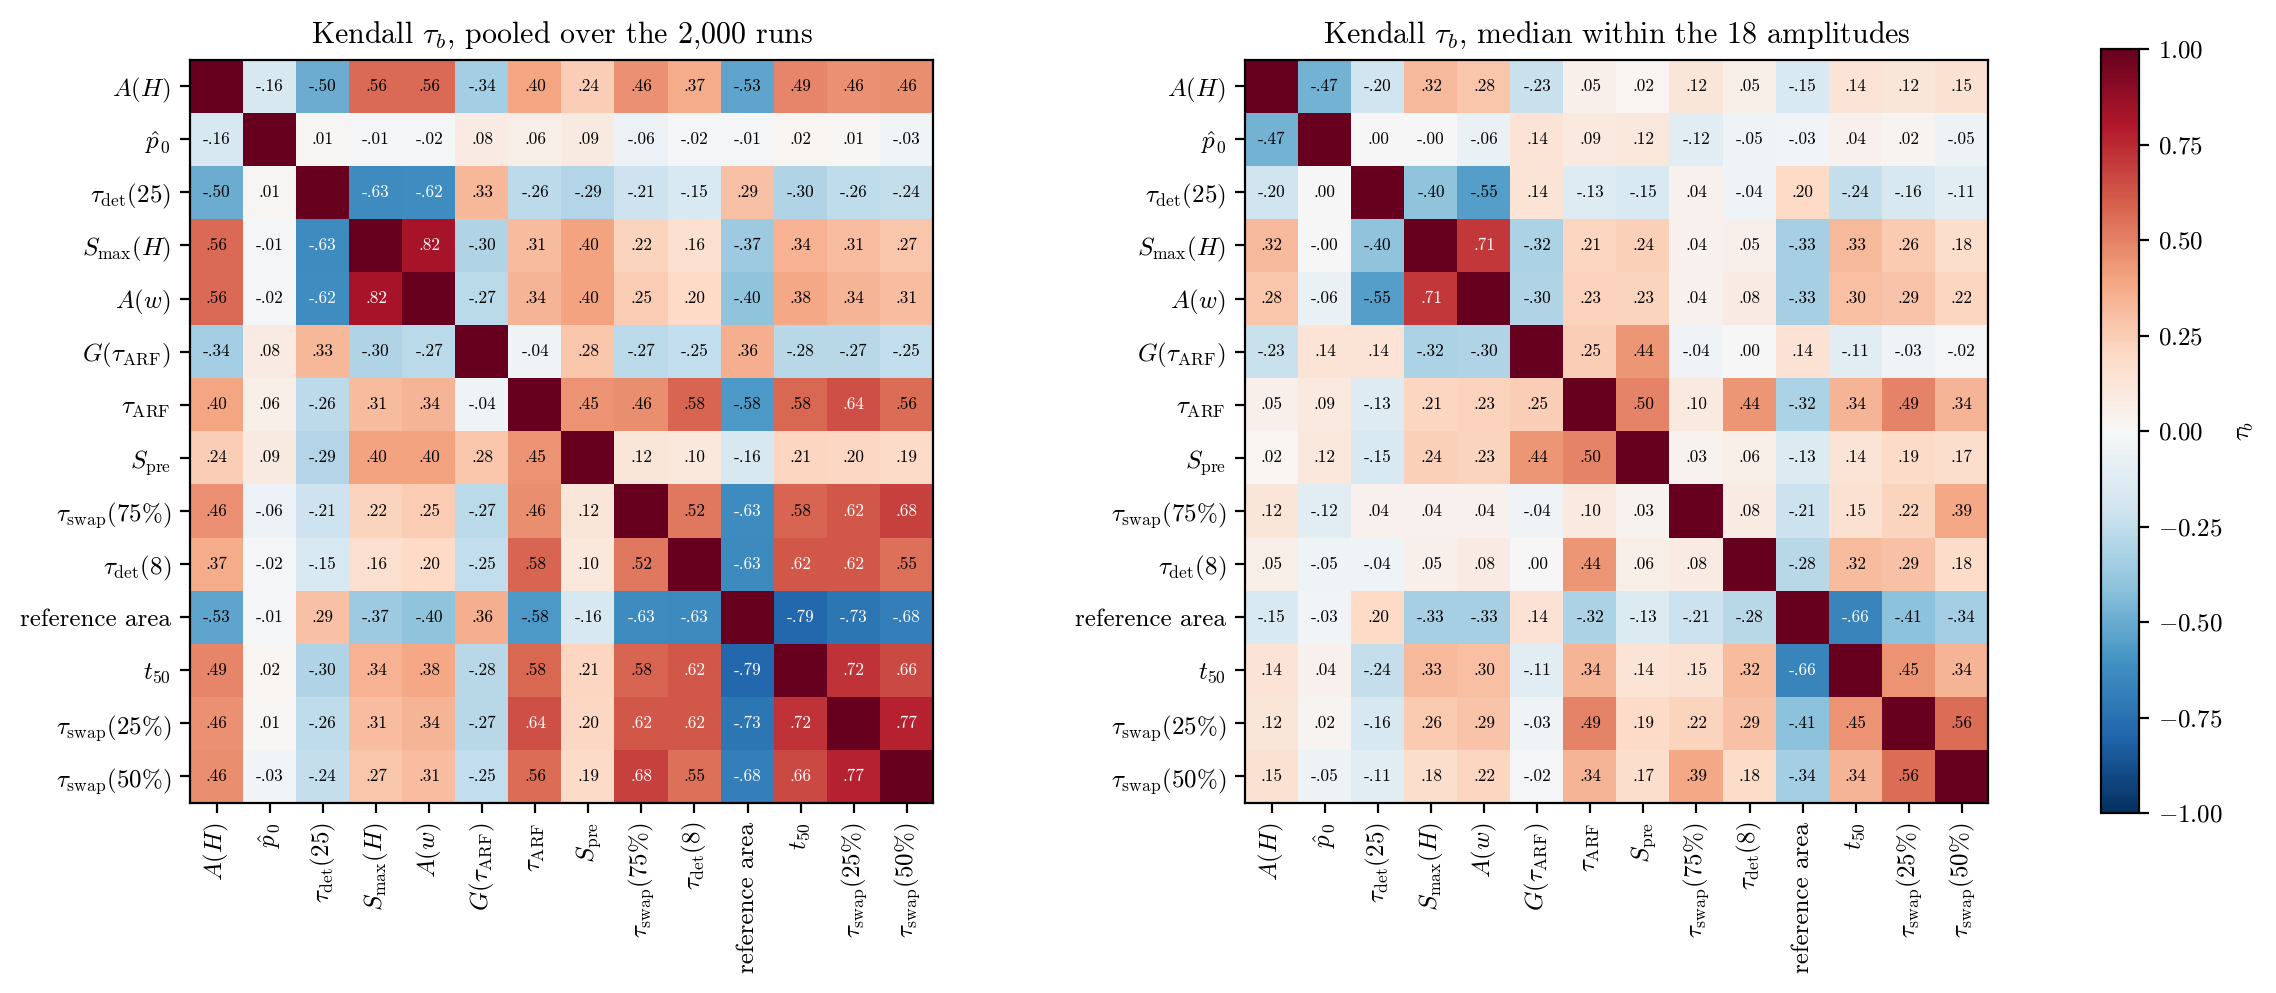
\includegraphics[width=0.86\textwidth]{Fig_QD_matrice_correlations_full.png}
  \end{center}
  \vspace{-0.5em}
  \small
  \begin{columns}[T,onlytextwidth]
    \begin{column}{0.32\textwidth}
      \textbf{Left, pooled:} almost everything agrees, because the drift size moves every
      indicator.
    \end{column}\hfill
    \begin{column}{0.32\textwidth}
      \textbf{Right, within a size:} two groups remain, \emph{evidence} ($0.71$) and
      \emph{repair}, weakly joined.
    \end{column}\hfill
    \begin{column}{0.32\textwidth}
      Best date against the analytic reference: \alert{3 trees replaced}, $0.45$, ahead of
      the first tree, $0.34$.
    \end{column}
  \end{columns}
  \note{To see all indicators at once, we crossed fourteen of them. The left panel pools all
    runs together: almost everything is strongly correlated with everything. That is an
    illusion, Simpson's paradox: the drift size moves every indicator, so pooling creates
    agreement. The right panel computes the same correlations within each drift size. Most of
    the agreement disappears, and two groups remain. One group measures evidence and damage:
    the detector's peak and the excess error over the transition agree strongly. The other
    group measures the repair. Between the two groups, links stay weak. We also compared the
    replacement dates with an analytic reference, the accuracy of the forest on the region
    whose label changed. The date at which three trees are replaced tracks it better than the
    first tree. This matrix is exploratory.}
\end{frame}

% =====================================================================
\section{III. Evidence vs threshold}
% =====================================================================

\begin{frame}{Part III --- Evidence against the threshold}
  \begin{center}\carte{3}\end{center}
  \note{The third part ties the first two together.}
\end{frame}

\begin{frame}{The race is decided before the repair}
  \begin{columns}[c,onlytextwidth]
    \begin{column}{0.52\textwidth}
      \centering
      \resizebox{\linewidth}{!}{\schemaidentite}\\
      {\scriptsize\color{gray} schematic}
    \end{column}\hfill
    \begin{column}{0.44\textwidth}
      A time counts observations; $\lambda$ counts \emph{excess errors}. Comparing them
      needs a rate that does not exist.
      \begin{block}{Race identity, on every run}
        \vspace{-0.4em}
        \[
          \tau_{\mathrm{det}} < \tau_{\mathrm{ARF}}
          \iff S_{\mathrm{pre}} \ge \lambda
        \]
        \vspace{-0.9em}
        \[
          S_{\mathrm{pre}} = \max_{t < \tau_{\mathrm{ARF}}} S_t
        \]
      \end{block}
      \small No rate, no averaging, no assumption on the trees. Checked on $2\,000$ runs out
      of $2\,000$ at three thresholds.
    \end{column}
  \end{columns}
  \note{Here is the key step. A repair time counts observations. A threshold counts excess
    errors. They are not in the same unit, and the paper bridges them with an average rate of
    errors per step. That rate does not exist: it falls as the forest repairs, and the
    detector forgets its evidence each time it hits zero. The exact statement is much
    simpler. Look at the statistic of the detector up to the first replacement, and take its
    highest point: we call it S pre. The detector arrives first if and only if S pre reaches
    the threshold. With a low threshold, it is reached before the repair; with a high one, it
    is not. This is exact on every run, it needs no rate, no averaging and no assumption on
    the trees, and we checked it on all two thousand runs.}
\end{frame}

\begin{frame}{The evidence before the repair sets the transition}
  \begin{columns}[c,onlytextwidth]
    \begin{column}{0.60\textwidth}
      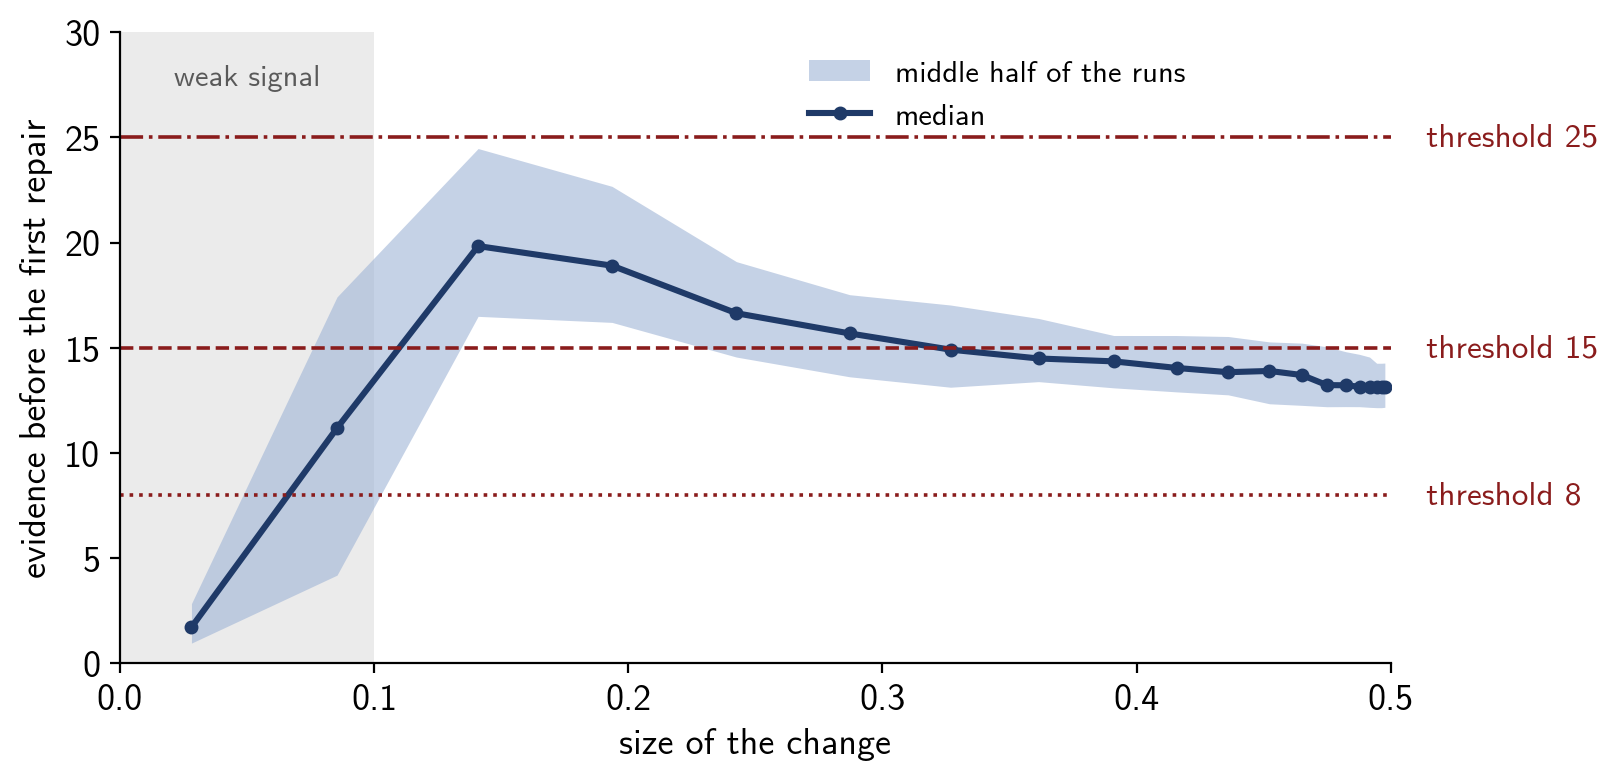
\includegraphics[width=\textwidth]{Fig_slide_spre.png}
    \end{column}\hfill
    \begin{column}{0.37\textwidth}
      \begin{itemize}
        \item Above the weak-signal zone, the median lies between \textbf{$13.1$ and $19.8$}:
              the transition the paper sees between $15$ and $25$, \alert{and leaves
              unexplained}.
        \item It \textbf{decreases} as the drift grows: at $\lambda = 15$ the detector wins
              $81\%$, then only $18\%$. That is the paradox.
      \end{itemize}
    \end{column}
  \end{columns}
  \note{So we measured S pre on every run. The dark line is the median by drift size, the band
    holds the middle half of the runs, and the red lines are thresholds. Above the weak-signal
    zone, the median sits between thirteen and twenty. A threshold below that level is reached
    before the repair in most runs; a threshold above it rarely is. That is exactly the
    transition the paper observes between fifteen and twenty-five, and leaves to future work.
    Now look at the shape. After the medium drifts, S pre decreases as the drift gets stronger,
    because the first replacement comes sooner. At a fixed threshold of fifteen, the detector
    wins eighty-one percent of the races on medium drifts, and only eighteen percent on the
    strongest ones. The paradox is this decreasing evidence, read against a fixed threshold. At
    the far left, the drift is too weak to accumulate anything: that is a different regime.}
\end{frame}

\begin{frame}{Stronger drifts leave no more evidence}
  \begin{columns}[c,onlytextwidth]
    \begin{column}{0.48\textwidth}
      \centering
      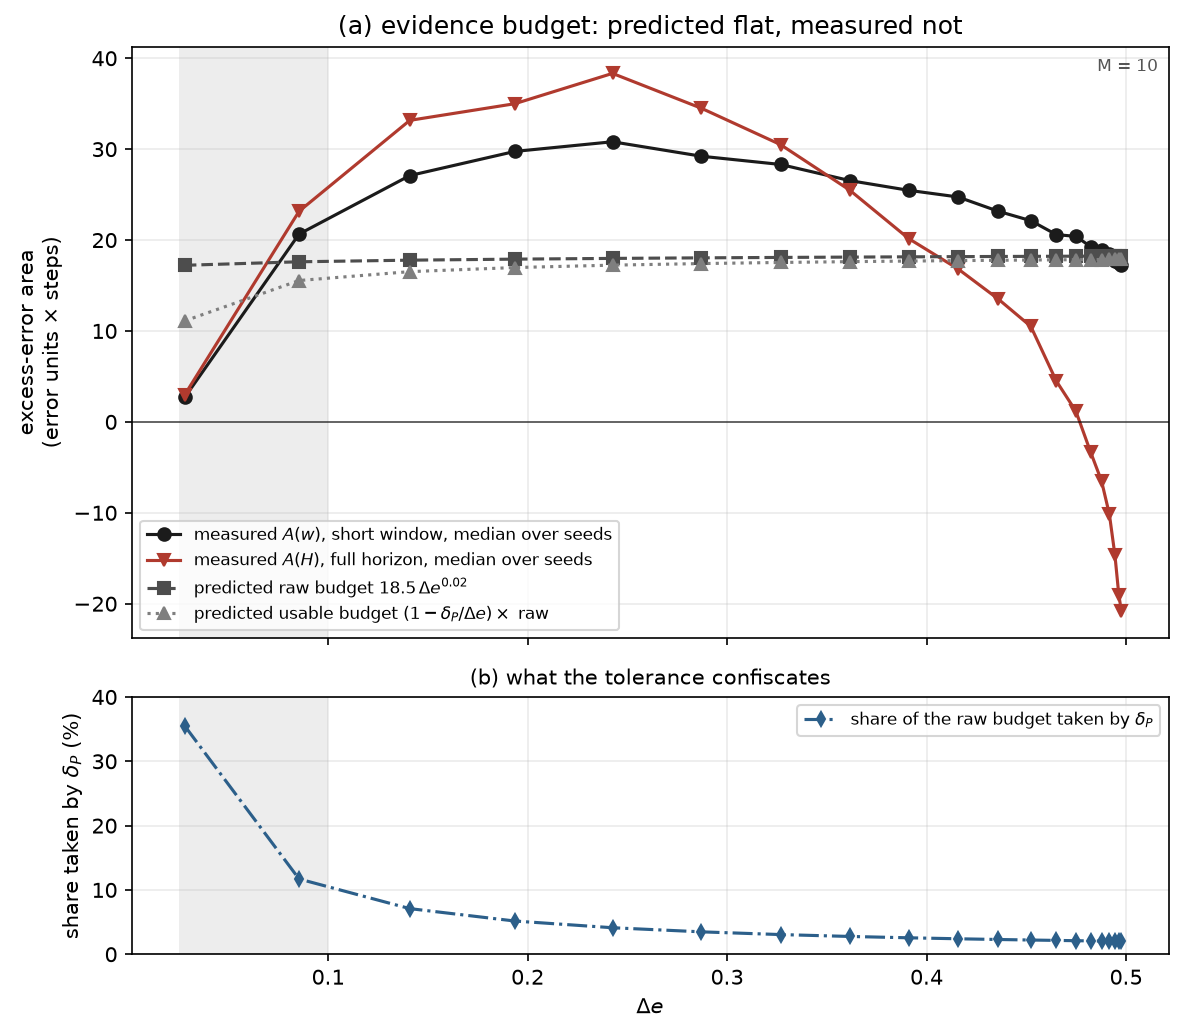
\includegraphics[height=0.66\textheight]{Fig_QC_budget_utilisable_full.png}
    \end{column}\hfill
    \begin{column}{0.46\textwidth}
      \begin{itemize}
        \item The paper's picture: an excess error $\Delta e$ over a window $\tau_{\mathrm{ARF}}$,
              so the area stays almost constant.
        \item Measured over the transition, the area varies by a factor of $1.8$ while the
              drift size varies by $5.8$: \alert{the compensation is real}.
        \item But the paper's rectangle misestimates it by up to $43\%$, and over the whole
              horizon the area turns negative at large drifts: the new task is easier.
      \end{itemize}
    \end{column}
  \end{columns}
  \note{Why doesn't a violent drift leave more evidence than a gentle one? The paper's picture
    is a rectangle: an excess error of height delta e, during a window equal to the repair
    time. Since the repair time shrinks like one over delta e, the area stays almost constant.
    We measured the area directly. Over the transition, it varies by a factor of less than two,
    while the drift size varies by almost six: the compensation is real. But the rectangle
    itself is wrong. It misestimates the area by up to forty-three percent, because the first
    replacement is not the width of the transient. And over the whole horizon, at large drifts,
    the area even becomes negative: after the change the task is easier than before, and the
    error settles below its old level. The evidence exists, it is roughly constant, but the
    paper's derivation of it does not hold.}
\end{frame}

\begin{frame}{Detecting is not winning}
  \begin{center}
    \begin{tabular}{@{}cccc@{}}
      \toprule
      threshold $\lambda$ & alarm fires & detector arrives first & false alarms, no drift \\
      \midrule
      $8$  & $95.3\%$ & $\mathbf{91.0\%}$ & $4.15\%$ \\
      $15$ & $92.9\%$ & $\mathbf{36.3\%}$ & $0.15\%$ \\
      $20$ & $66.2\%$ & $8.1\%$           & $0.00\%$ \\
      $25$ & $38.9\%$ & $2.5\%$           & $0.00\%$ \\
      \bottomrule
    \end{tabular}\\[0.3em]
    {\scriptsize\color{gray} $2\,000$ runs with drift and $2\,000$ without, over $2\,000$ steps}
  \end{center}
  \begin{itemize}
    \item At $\lambda = 15$ the alarm almost always fires, but mostly \emph{after} the repair.
    \item At $\lambda = 8$ the detector wins at an ordinary false-alarm cost: the paper's
          ``no threshold escapes'' does not hold on this bench.
    \item \textcolor{gray}{Not tested: the heteroscedastic streams where the paper places its
          false-alarm tension.}
  \end{itemize}
  \note{One practical consequence. Detecting a drift and winning the race are two different
    things. At threshold fifteen, the alarm fires on ninety-three percent of drifts, which
    looks excellent, but it arrives before the repair in only thirty-six percent of them.
    Most of these alarms come after the forest has already changed. At threshold eight, the
    detector wins ninety-one percent of the races, and it costs about four percent of false
    alarms over two thousand steps where nothing happens, which is an ordinary calibration
    level. So on this bench, one threshold does escape the blind spot, and the paper's claim
    that no threshold escapes has to be restricted. We did not test the financial streams
    with clustered volatility, where the paper places the false-alarm problem.}
\end{frame}

% =====================================================================
\section{Conclusion}
% =====================================================================

\begin{frame}{What changes in the paper}
  \small
  \begin{tabular}{@{}p{0.34\textwidth}p{0.43\textwidth}l@{}}
    \toprule
    The paper & Our result & \\
    \midrule
    races the repair against a constant & race identified, bounded, decided run by run & \textbf{made exact} \\
    independent trees, bias asserted & direction proven, cannot reverse & \textbf{proven} \\
    error back to normal at the first replacement & it comes back later; the rectangle fails & \textbf{corrected} \\
    first replacement as the repair date & earliest date, fires without drift & \textbf{qualified} \\
    transition between $15$ and $25$, unexplained & set by the evidence before the repair & \textbf{explained} \\
    no threshold escapes & $\lambda = 8$ does, on this bench & \textbf{restricted} \\
    \bottomrule
  \end{tabular}
  \vspace{0.6em}
  \begin{center}
    \alert{The phenomenon survives. What changes is its mechanism and its reach.}
  \end{center}
  \note{To sum up what our work changes in the paper. The race, which compared a random time
    with a constant, is made exact: identified, bounded, and decided run by run. The bias of
    the independence assumption was asserted; it is now proven, with its direction. The idea
    that the error is back to normal at the first replacement is corrected. The first
    replacement as a repair date is qualified: it is the earliest date and it fires without
    drift. The transition threshold, which the paper left unexplained, is explained by the
    evidence before the repair. And the claim that no threshold escapes is restricted to the
    settings the paper actually tested. The phenomenon survives all of this. What changes is
    its mechanism, and its reach.}
\end{frame}

\begin{frame}{An open question, and what we did not do}
  \begin{columns}[T,onlytextwidth]
    \begin{column}{0.50\textwidth}
      \begin{exampleblock}{Open: a reference for adaptation}
        Every indicator on the detector's side reads the \emph{error}, which mixes what the
        forest relearned with how hard the new task is. On analytic probes, the forest can
        relearn the changed region and lose a rare one, unseen by the error.
      \end{exampleblock}
    \end{column}\hfill
    \begin{column}{0.46\textwidth}
      \begin{block}{Not done}
        \small
        \begin{itemize}
          \item one forest size, one homoscedastic bench
          \item decision rule fixed during the analysis
          \item the independence bias has a sign, not a size
        \end{itemize}
      \end{block}
    \end{column}
  \end{columns}
  \note{We leave one question open. Every measure available to the detector reads the error,
    and the error mixes two things: what the forest has relearned, and how hard the new task
    is. Using analytic probes, points whose true label we know, we saw that the forest can
    relearn the region that changed while losing a rare region elsewhere, and the error does
    not see that loss. So what would a true reference for adaptation be? We do not have the
    answer. And to be honest about the limits: we studied one forest size on one simple
    bench, our decision rule was fixed during the analysis rather than before it, and we can
    give the sign of the independence bias but not its size.}
\end{frame}

\begin{frame}{Take-away}
  \begin{center}
    \small\alert{The blind spot is a budget of evidence, accumulated before the repair, set
    against a threshold.}
  \end{center}
  \vspace{-0.5em}
  \begin{center}\carte[0.71]{0}\end{center}
  \note{Back to the map. The blind spot is real, and it survives every correction. But it is
    not a race between two clocks. It is the evidence the forest lets through before its first
    repair, set against a fixed threshold. That single quantity explains when the detector
    wins, why the transition sits where it does, and why stronger drifts are missed more
    often. Thank you for your attention; we are happy to take your questions.}
\end{frame}

% =====================================================================
\appendix
\section*{Backup}
% =====================================================================

\begin{frame}{Backup --- Fréchet bounds}
  For integer-valued clocks with marginal CDFs $F_A$ and $F_D$, and \emph{any} coupling,
  \begin{align*}
    P_{\mathrm{miss}} &\ge \max\Big(0,\ \sup_{s} \big[F_A(s)-F_D(s)\big]\Big),\\
    P_{\mathrm{miss}} &\le \min\Big(1,\ \inf_{s} \big[F_A(s) + 1 - F_D(s+1)\big]\Big).
  \end{align*}
  \begin{itemize}
    \item Lower: Fréchet on $\{\tau_{\mathrm{ARF}} \le s < \tau_{\mathrm{det}}\} \subseteq \mathrm{Miss}$.
    \item Upper: $\mathrm{Miss} \subseteq \{\tau_{\mathrm{ARF}} \le s\} \cup \{\tau_{\mathrm{det}} > s+1\}$, then Boole.
    \item Toy case, both clocks uniform on $\{1,2\}$: the bounds $0$ and $0.5$ are both attained.
  \end{itemize}
\end{frame}

\begin{frame}{Backup --- Lindley's closed form and the certificate}
  With $X_t = e_t - \hat p_0 - \delta_P$ and $A(k,j) = \sum_{t=k+1}^{j} (e_t - \hat p_0)$,
  \[
    S_j = \max_{0 \le k \le j} \sum_{t=k+1}^{j} X_t,
    \qquad
    S_{\max}(H) = \max_{0 \le k \le j \le H} \big[A(k,j) - (j-k)\,\delta_P\big].
  \]
  \begin{itemize}
    \item Certificate: the alarm fires by $H$ iff some sub-window carries
          $A(k,j) \ge \lambda + (j-k)\,\delta_P$. The full window alone is only sufficient.
    \item Race identity: the same maximum, taken up to the first replacement, is $S_{\mathrm{pre}}$.
  \end{itemize}
\end{frame}

\begin{frame}{Backup --- Association protocol}
  \begin{itemize}
    \item Every coefficient is computed \textbf{within a drift size} ($100$ seeds), on the $18$
          sizes with $\Delta e \ge 0.10$: pooling measures the drift size, not the link.
    \item Kendall's $\tau_b$: reads on pairs, corrects for ties. Censored durations ranked last,
          licit because the horizon is common to all runs.
    \item Pearson undefined on censored values; Spearman handles their ties implicitly.
    \item Percentile bootstrap over seeds, $2\,000$ resamples; discernible if the interval
          excludes zero. Fixed during the analysis, not before: stated in the report.
    \item Complete cases instead of ranking censored runs last: no coefficient moves by more
          than $0.0403$.
  \end{itemize}
\end{frame}

\begin{frame}{Backup --- The drift-free control}
  \begin{center}
    \begin{tabular}{@{}lr@{}}
      \toprule
      On $2\,000$ runs with no change point & \\
      \midrule
      runs where at least one tree is replaced & $2\,000/2\,000$ \\
      first replacement, median & $95$ steps \\
      distinct trees renewed, median & $9/10$ \\
      forest entirely renewed & $28.7\%$ \\
      \midrule
      first replacement at the weakest drift, median & $118$ steps \\
      \bottomrule
    \end{tabular}
  \end{center}
\end{frame}

\end{document}
"
%
% Tracabilite : chaque chiffre vient du rapport ; controle par
%   verif_chiffres_tex.py ../../05_presentation/soutenance_20min.tex
% Figures : figures_slides.py --latex, figures_soutenance.py,
%   matrice_correlations.py, analyse_QCD.py (budget).
% =====================================================================

\documentclass[aspectratio=169,11pt]{beamer}

\usetheme{Madrid}
% Rouge de CentraleSupelec, pris dans le logo officiel (#B00739) ; logo
% CentraleSupelec / Universite Paris-Saclay sur la page de titre.
\definecolor{csRouge}{HTML}{B00739}
\usecolortheme[named=csRouge]{structure}
\setbeamercolor{alerted text}{fg=csRouge}
\setbeamersize{text margin left=1cm, text margin right=1cm}
\setbeamertemplate{navigation symbols}{}
\usepackage[english]{babel}
\usepackage{amsmath,amssymb}
\usepackage{graphicx}
\usepackage{booktabs}
\usepackage{tikz}
% soutenance_schemas.tex
% =====================================================================
% Schemas TikZ de `soutenance_20min.tex` : la carte des idees et le schema
% de l'identite de course.
%
% Fichier separe pour la meme raison que `point_encadrant_schemas.tex` :
% `verif_chiffres_tex.py` ramasserait les coordonnees TikZ comme des mesures.
% AUCUN chiffre de mesure ici ; les schemas sont stylises, sans donnees.
% =====================================================================

\usetikzlibrary{positioning, arrows.meta, calc}

\definecolor{mTheorie}{RGB}{31,58,104}
\definecolor{mDate}{RGB}{138,28,28}
\definecolor{mPreuve}{RGB}{38,92,58}
\definecolor{mEteint}{gray}{0.74}

% ---------------------------------------------------------------------
% \carte[hauteur]{k} : la carte des idees.
%   k = 0 : tout est actif (ouverture et conclusion)
%   k = 1, 2, 3 : seule la partie k est en couleur, le reste est grise
%   hauteur : fraction de \textheight (0.80 par defaut)
% Les fleches en pointille relient les parties ; elles sont commentees a
% l'oral plutot qu'etiquetees, faute de place entre les colonnes.
% ---------------------------------------------------------------------
\newcommand{\carte}[2][0.80]{%
  \colorlet{cUn}{mEteint}\colorlet{cDeux}{mEteint}\colorlet{cTrois}{mEteint}%
  \colorlet{tUn}{mEteint}\colorlet{tDeux}{mEteint}\colorlet{tTrois}{mEteint}%
  \ifnum#2=0 \colorlet{cUn}{mTheorie}\colorlet{cDeux}{mDate}\colorlet{cTrois}{mPreuve}%
    \colorlet{tUn}{black}\colorlet{tDeux}{black}\colorlet{tTrois}{black}\fi
  \ifnum#2=1 \colorlet{cUn}{mTheorie}\colorlet{tUn}{black}\fi
  \ifnum#2=2 \colorlet{cDeux}{mDate}\colorlet{tDeux}{black}\fi
  \ifnum#2=3 \colorlet{cTrois}{mPreuve}\colorlet{tTrois}{black}\fi
  \resizebox{!}{#1\textheight}{%
  \begin{tikzpicture}[
      font=\normalsize, align=center,
      boite/.style={draw, line width=1pt, rounded corners=3pt, inner sep=4pt,
                    text width=4.3cm, minimum height=1.05cm},
      un/.style={boite, draw=cUn, text=tUn},
      deux/.style={boite, draw=cDeux, text=tDeux},
      trois/.style={boite, draw=cTrois, text=tTrois},
      tete/.style={font=\bfseries\normalsize, text width=4.8cm},
      fl/.style={-{Stealth[length=2.4mm]}, line width=0.9pt},
      lien/.style={-{Stealth[length=2.4mm]}, line width=0.9pt, dashed},
    ]
    \node[boite, draw=black, fill=black!4, text width=12cm, minimum height=0.8cm] (P) at (5.6,0.15)
      {\textbf{The paper:} the stronger the drift, the faster the repair, the fewer the alarms};

    \node[tete, text=cUn]    (H1) at (0,-1.05)    {I.\ The race, formally};
    \node[tete, text=cDeux]  (H2) at (5.6,-1.05)  {II.\ The repair date};
    \node[tete, text=cTrois] (H3) at (11.2,-1.05) {III.\ Evidence vs threshold};
    \draw[fl, black!55] (P.south) -- ++(0,-0.25) -| (H1.north);
    \draw[fl, black!55] (P.south) -- (H2.north);
    \draw[fl, black!55] (P.south) -- ++(0,-0.25) -| (H3.north);

    \node[un] (A1) at (0,-2.1)  {The miss is well defined, its probability identified};
    \node[un] (A2) at (0,-3.45) {The blind spot holds whatever the dependence};
    \node[un] (B1) at (0,-4.8)  {Independent trees overstate the speed of repair};

    \node[deux] (C1) at (5.6,-2.1)  {The first replacement is the earliest date};
    \node[deux] (E1) at (5.6,-3.45) {It fires as fast when nothing changes};
    \node[deux] (D1) at (5.6,-4.8)  {When it fires, half the evidence is there};
    \node[deux] (D2) at (5.6,-6.15) {Indicators form two groups, weakly linked};

    \node[trois] (C2) at (11.2,-2.1)  {The alarm is a function of the error path};
    \node[trois] (K)  at (11.2,-3.45) {Detector first \emph{iff} it reaches $\lambda$ before the repair};
    \node[trois] (S)  at (11.2,-4.8)  {That evidence sets the transition and the paradox};
    \node[trois] (T)  at (11.2,-6.15) {Detecting is not winning};

    \node[boite, draw=black!55, text=black!80, dashed, text width=7cm, minimum height=0.8cm] (O) at (5.6,-7.45)
      {\textbf{Open:} a reference for adaptation itself};

    \draw[fl, cUn]    (A1) -- (A2);
    \draw[fl, cDeux]  (C1) -- (E1);
    \draw[fl, cDeux]  (E1) -- (D1);
    \draw[fl, cDeux]  (D1) -- (D2);
    \draw[fl, cTrois] (C2) -- (K);
    \draw[fl, cTrois] (K) -- (S);
    \draw[fl, cTrois] (S) -- (T);
    \draw[lien, black!55] (B1.east) -- (D1.west);
    \draw[lien, black!55] (D1.east) -- (S.west);
    \draw[lien, black!55] (D2.south) -- (O.north);
  \end{tikzpicture}}%
}

% ---------------------------------------------------------------------
% \schemaidentite : la pile S_t, le premier remplacement, deux seuils.
% Stylise, sans donnees.
% ---------------------------------------------------------------------
\newcommand{\schemaidentite}{%
  \begin{tikzpicture}[x=1cm, y=1cm, font=\small]
    \draw[-{Stealth}, line width=0.7pt] (0,0) -- (7.2,0);
    \node[below left] at (7.2,-0.05) {time};
    \draw[-{Stealth}, line width=0.7pt] (0,0) -- (0,3.7);
    \node[rotate=90, above] at (-0.05,1.85) {detector statistic $S_t$};
    \draw[line width=1.4pt, mTheorie]
      (0,0) .. controls (0.8,0.6) and (1.6,1.9) .. (2.4,2.25)
            .. controls (3.0,2.5) and (3.4,2.55) .. (3.9,2.4)
            .. controls (4.8,2.0) and (5.8,1.0) .. (7.0,0.3);
    \draw[dashed, mDate, line width=1pt] (2.8,0) -- (2.8,3.4);
    \node[above, text=mDate] at (2.8,3.4) {first replacement};
    \fill[mTheorie] (2.8,2.38) circle (2.3pt);
    \node[above left, text=mTheorie] at (2.75,2.4) {$S_{\mathrm{pre}}$};
    \draw[mPreuve, line width=1pt] (0,1.5) -- (7.0,1.5);
    \node[above left, text=mPreuve] at (7.0,1.5) {low $\lambda$: reached before};
    \draw[mDate, line width=1pt, dash dot] (0,3.0) -- (7.0,3.0);
    \node[above left, text=mDate] at (7.0,3.0) {high $\lambda$: not reached};
  \end{tikzpicture}%
}

\titlegraphic{
\includegraphics[height=1.7cm]{Logo_CS_Paris_Saclay.png}}
\ifdefined\NOTESSEULES\setbeameroption{show only notes}\fi
\graphicspath{{../04_experimentations/resultats_R2/resultats/figures/slides_latex/}{../04_experimentations/resultats_R2/resultats/figures/}}

\setbeamerfont{author}{size=\small}
\setbeamerfont{institute}{size=\scriptsize}

\title[The Blind Spot Paradox]{The Blind Spot Paradox}
\subtitle{Formalizing the race and measuring the adaptation}
\author[Boyer, Gouillou, Fonvielle, Petit-Tichanné]{Alexandre Boyer \and Melaine Gouillou \and Salomé Fonvielle \and Ulysse Petit-Tichanné}
\institute[CS]{Research Track, Topic 39, CentraleSupélec. Supervisor: Raphaël Minato}
\date{16 September 2026}

\begin{document}

\maketitle
\note{Good afternoon. Our subject is the blind spot paradox: a model that repairs
  itself can destroy the very evidence its own monitor needs. In the next twenty
  minutes we will present what we formalized, what we measured, and the single
  reading that ties the two together.}

% =====================================================================
\section{The problem}
% =====================================================================

\begin{frame}{Concept drift: the rule changes, the data does not}
  \vspace{-0.6em}
  \[
    \underbrace{P(X)}_{\text{the data}}\ \text{unchanged}
    \qquad\qquad
    \underbrace{P(Y \mid X)}_{\text{the rule}}\ \text{changes}
  \]
  \vspace{-0.9em}
  \begin{center}
    
\includegraphics[height=0.50\textheight]{Fig_slide_drift.png}
  \end{center}
  \begin{center}
    A model trained before the change is now \alert{wrong on the shaded band}.
  \end{center}
  \note{A classifier learns a rule from data. In a data stream, that rule can change
    while the inputs keep exactly the same distribution. This is concept drift: P of X
    does not move, P of Y given X does. It is the normal situation for a financial
    signal, where the same inputs stop meaning the same thing. In the bench we use,
    points in the plane are separated by a line. At the change, the line moves. Every
    point in the shaded band switches label, so a model trained before the change keeps
    predicting confidently, and is now wrong on that band. The size of the band is the
    size of the drift, written delta e.}
\end{frame}

\begin{frame}{Two defences that run at the same time}
  \begin{columns}[T,onlytextwidth]
    \begin{column}{0.49\textwidth}
      \centering
      \textbf{The model repairs itself}\\[0.3em]
      
\includegraphics[width=\textwidth]{Fig_slide_foret.png}\\[0.2em]
      \small Adaptive Random Forest: ten trees, each replaced when its own error rises.
    \end{column}\hfill
    \begin{column}{0.49\textwidth}
      \centering
      \textbf{A monitor raises the alarm}\\[0.3em]
      
\includegraphics[width=\textwidth]{Fig_slide_watchdog.png}\\[0.2em]
      \small Each error adds to a statistic $S_t$; the alarm fires when it crosses $\lambda$.
    \end{column}
  \end{columns}
  \note{Two defences are deployed together. The first one lives inside the model. The
    Adaptive Random Forest is made of ten decision trees that vote. Each tree watches its
    own error with a small detector, and when that error rises, the tree is replaced by a
    fresh one. The forest repairs itself locally, without asking anyone. The second defence
    sits outside. A cumulative detector, a Page-Hinkley test, watches the error of the
    whole forest. Every error pushes a statistic up by almost one, every correct answer
    pulls it down a little, never below zero. When the statistic crosses a threshold
    lambda, the alarm fires, and that alarm is the only thing a human operator sees.}
\end{frame}

\begin{frame}{The paradox, and what the reviewers asked}
  \begin{columns}[c,onlytextwidth]
    \begin{column}{0.50\textwidth}
      \centering
      
\includegraphics[width=\textwidth]{Fig_slide_mecanisme.png}\\
      {\scriptsize\color{gray} schematic}
    \end{column}\hfill
    \begin{column}{0.46\textwidth}
      \begin{block}{The paper's claim}
        The stronger the drift, the faster the repair, and the \alert{fewer} alarms.
      \end{block}
      \begin{alertblock}{Two corrections requested}
        \begin{enumerate}
          \item It races a random repair time against a \emph{constant}, and assumes the
                trees independent.
          \item It dates the repair at the \emph{first} tree replaced, without showing
                that this date means anything.
        \end{enumerate}
      \end{alertblock}
    \end{column}
  \end{columns}
  \note{When both defences run together, something unexpected happens. The drift starts,
    errors pile up in the detector, but the forest replaces trees, the errors stop, and the
    pile drains before it reaches the threshold. The paper we study calls this the blind
    spot paradox: the stronger the drift, the faster the forest repairs itself, and the
    fewer alarms the operator gets. The paper was reviewed, and two corrections were
    requested. First, it compares a random repair time with a constant detection time, and
    it assumes the ten trees are independent without proving it. Second, it dates the repair
    at the moment the first tree is replaced, without showing that this moment has anything
    to do with the error disappearing. These two corrections are where our work starts.}
\end{frame}

\begin{frame}{Our reading, in one map}
  \begin{center}
    \small\alert{The blind spot is not a race between two clocks,
    but a budget of evidence set against a threshold.}
  \end{center}
  \vspace{-0.5em}
  \begin{center}
    \carte[0.71]{0}
  \end{center}
  \note{Here is the whole talk on one map. At the top, the claim of the paper. The first
    column formalizes the race: we define the blind spot properly, we compute its
    probability, and we show that assuming independent trees makes the paper optimistic
    about the repair. The second column asks what the repair date really measures: it is
    the earliest possible date, it fires even when nothing changes, and when it fires most
    of the evidence is already there. The third column ties both together: the detector wins
    exactly when its evidence reaches the threshold before the repair, and that evidence
    explains both the transition and the paradox. The dashed arrows are the links between
    columns, and the box at the bottom is the question we leave open. Our one-sentence
    reading: the blind spot is not a race between two clocks, it is a budget of evidence set
    against a threshold.}
\end{frame}

% =====================================================================
\section{I. The race}
% =====================================================================

\begin{frame}{Part I --- The race, formally}
  \begin{center}\carte{1}\end{center}
  \note{Let us start with the theory: how to state the race without cheating.}
\end{frame}

\begin{frame}{The race is well posed, and its probability identified}
  \begin{columns}[T,onlytextwidth]
    \begin{column}{0.46\textwidth}
      \begin{block}{One definition, no ad hoc rule}
        \[
          \mathrm{Miss} := \{\tau_{\mathrm{ARF}} < \tau_{\mathrm{det}}\}
        \]
        \vspace{-0.6em}
        {\small strict inequality; the alarm may never come}
        \begin{itemize}
          \item a tie goes to the detector
          \item a silent repair, with no alarm ever, \alert{is} a miss
          \item if neither acts, it is not
        \end{itemize}
      \end{block}
    \end{column}\hfill
    \begin{column}{0.50\textwidth}
      \begin{exampleblock}{What the campaign allows}
        The forest always replaces a tree within the horizon, so no run is left
        undecided: $P_{\mathrm{miss}}$ is \textbf{identified}.\\[0.3em]
        \centering
        \begin{tabular}{@{}lccc@{}}
          $\lambda$ & $8$ & $25$ & $50$ \\
          $P_{\mathrm{miss}}$ & $0.0905$ & $0.9715$ & $1.0000$
        \end{tabular}
      \end{exampleblock}
      \begin{alertblock}{Without any dependence assumption}
        From the marginal laws alone, the blind spot at the weakest drift is at least
        $0.91$ at $\lambda = 8$.
      \end{alertblock}
    \end{column}
  \end{columns}
  \note{The paper says there is a blind spot when the forest repairs before the alarm, but
    it quietly sets aside the runs where the alarm never comes. Those are exactly the runs
    where the detector fails most. So we define the event on the complete race, with one
    definition and no extra rule. A tie counts for the detector, because the operator is
    warned at the right moment. A silent repair, where the alarm never comes, is a miss, and
    in fact the purest one. A run where neither mechanism acts is not a miss, because there
    was nothing to erase. Then comes the problem of the finite horizon: some runs could be
    undecided. On our campaign they are not, because the forest always acts within the
    horizon, so the miss probability is identified exactly: nine percent at threshold eight,
    ninety-seven at twenty-five, one hundred at fifty. And with Fréchet bounds, which use the
    two marginal laws and assume nothing on how the clocks are coupled, the blind spot at the
    weakest drift is already forced above ninety percent.}
\end{frame}

\begin{frame}{Trees share a stream: the paper is optimistic}
  \begin{enumerate}
    \item \textbf{Given the stream}, what separates two trees is their own random draws:
          the trees are independent \emph{conditionally}.
    \item \textbf{Averaging over streams}, convexity gives the direction:
          \[
            P(\tau_{\mathrm{ARF}} \le s) \;\le\; 1 - \big(1 - F(s)\big)^M
          \]
          \alert{The independence formula overstates the speed of the repair.}
    \item \textbf{Consequence}: the paper's critical ensemble size becomes a conservative
          ceiling; its verdict does not change.
    \item \textbf{No coupling reverses the sign}: sharing a stream can only make trees fail
          together, since the covariance equals a variance.
  \end{enumerate}
  \note{The second shortcut is independence. The ten trees learn from the same stream, so
    they cannot be independent. But the question is at which level. Once the stream is
    fixed, what distinguishes one tree from another is only its own randomness, the random
    weights of online bagging. At that level, given the stream, the trees are independent.
    When we average over streams, Jensen's inequality gives a clear direction: the
    probability that the forest has already repaired itself is at most what the independence
    formula predicts. So the paper makes the forest look faster than it is, and overestimates
    the blind spot. Its critical ensemble size is not wrong, it becomes a conservative
    ceiling, and the paper's own verdict does not change. Could dependence go the other way?
    No: the covariance between two trees equals a variance, so it is never negative.}
\end{frame}

% =====================================================================
\section{II. The repair date}
% =====================================================================

\begin{frame}{Part II --- What the repair date measures}
  \begin{center}\carte{2}\end{center}
  \note{Now the second correction: the date the paper uses for the repair.}
\end{frame}

\begin{frame}{How we measured}
  \begin{columns}[T,onlytextwidth]
    \begin{column}{0.48\textwidth}
      \begin{block}{The campaign}
        \begin{itemize}
          \item the paper's bench, rerun: $20$ drift sizes $\times$ $100$ seeds,
                $2\,000$ steps after the change
          \item $2\,000$ more runs with no change at all
          \item only the error and the replacement events are recorded; every threshold is
                replayed offline
        \end{itemize}
      \end{block}
    \end{column}\hfill
    \begin{column}{0.48\textwidth}
      \begin{block}{Reading an association}
        \begin{itemize}
          \item always \alert{within one drift size}: pooling measures the drift size, not
                the link
          \item Kendall's rank correlation, with bootstrap intervals over the seeds
          \item steps added after seeing the data are flagged as exploratory
        \end{itemize}
      \end{block}
    \end{column}
  \end{columns}
  \note{A word on how we measured, without the implementation details. We reran the bench
    of the paper on twenty drift sizes, with one hundred seeds each, and we observe two
    thousand steps after the change. We added two thousand runs where nothing changes at
    all, as a control. The simulation records only two things: the error at each step and
    the moments when trees are replaced. Everything else, including the detector at any
    threshold, is recomputed offline, so one campaign replaces many. When we correlate two
    quantities, we always do it within one drift size. The drift size moves every indicator
    at once, so a correlation pooled over sizes mostly measures the size itself. We use
    Kendall's rank correlation with bootstrap intervals, and we flag the steps we added
    after looking at the data.}
\end{frame}

\begin{frame}{The first replacement is the earliest possible date}
  \begin{center}
    
\includegraphics[width=0.90\textwidth]{Fig_slide_deux_horloges.png}
  \end{center}
  \vspace{-0.3em}
  \begin{itemize}
    \item On every run, the first replacement comes before any other quota of renewed
          trees. Three quarters of the forest are renewed \textbf{$6.0$ to $14.3$ times later}.
    \item \alert{With no drift at all}, the first replacement comes after $95$ steps in
          median, against $118$ on the weakest drift.
  \end{itemize}
  \note{The paper dates the repair at the first replaced tree. By construction, that is the
    earliest of all possible dates: the moment when three trees, or half, or three quarters
    of the forest are replaced, always comes later, on every run. The only question is how
    much later. On this medium drift, the first tree goes after eighty-six observations, and
    three quarters of the forest after more than twelve hundred. Over the grid, three
    quarters of the forest are renewed six to fourteen times later than the first tree. And
    there is a more worrying fact. On the two thousand runs with no change at all, the forest
    still replaces its first tree, after ninety-five steps in median. On the weakest real
    drift, it takes one hundred and eighteen. So at low drift, this date cannot tell a real
    change from noise.}
\end{frame}

\begin{frame}{When the first tree goes, most of the evidence is already there}
  \begin{columns}[T,onlytextwidth]
    \begin{column}{0.36\textwidth}
      \begin{block}{Evidence at the first replacement}
        \centering
        {\Large $49\%$ to $76\%$}\\[0.2em]
        \small of the detector's final peak, on the $18$ drift sizes studied
      \end{block}
    \end{column}\hfill
    \begin{column}{0.60\textwidth}
      \begin{block}{Does the date track anything, within a drift size?}
        \small
        \begin{tabular}{@{}lcc@{}}
          \toprule
          compared with & median link & sizes \\
          \midrule
          detector peak & $0.21$ & $15/18$ \\
          excess error, whole horizon & none & $0/18$ \\
          excess error, transition only & $0.23$ & $13/18$ \\
          \bottomrule
        \end{tabular}
      \end{block}
    \end{column}
  \end{columns}
  \vspace{0.8em}
  \begin{center}
    \small The null over the whole horizon is mostly noise: \alert{half} of that area's
    variance comes from the estimated baseline, multiplied by the horizon.
  \end{center}
  \note{Is the first replacement at least the end of the transient? No. When the first tree
    is replaced, the detector already holds between half and three quarters of all the
    evidence it will ever accumulate. The replacement is in the middle of the story, not at
    its end. Then we asked whether this date tracks anything, always within a drift size.
    With the peak of the detector, there is a weak but real link, visible on fifteen drift
    sizes out of eighteen. With the excess error over the whole horizon, there is no link at
    all. But we found out why: that area adds up two thousand steps, so any error on the
    baseline is multiplied by two thousand, and half of its variance is just that noise. If
    we keep only the transition, the link comes back, weak but real, on thirteen sizes out of
    eighteen. This last step is exploratory.}
\end{frame}

\begin{frame}{Unexpected: pooling manufactures agreement}
  \begin{center}
    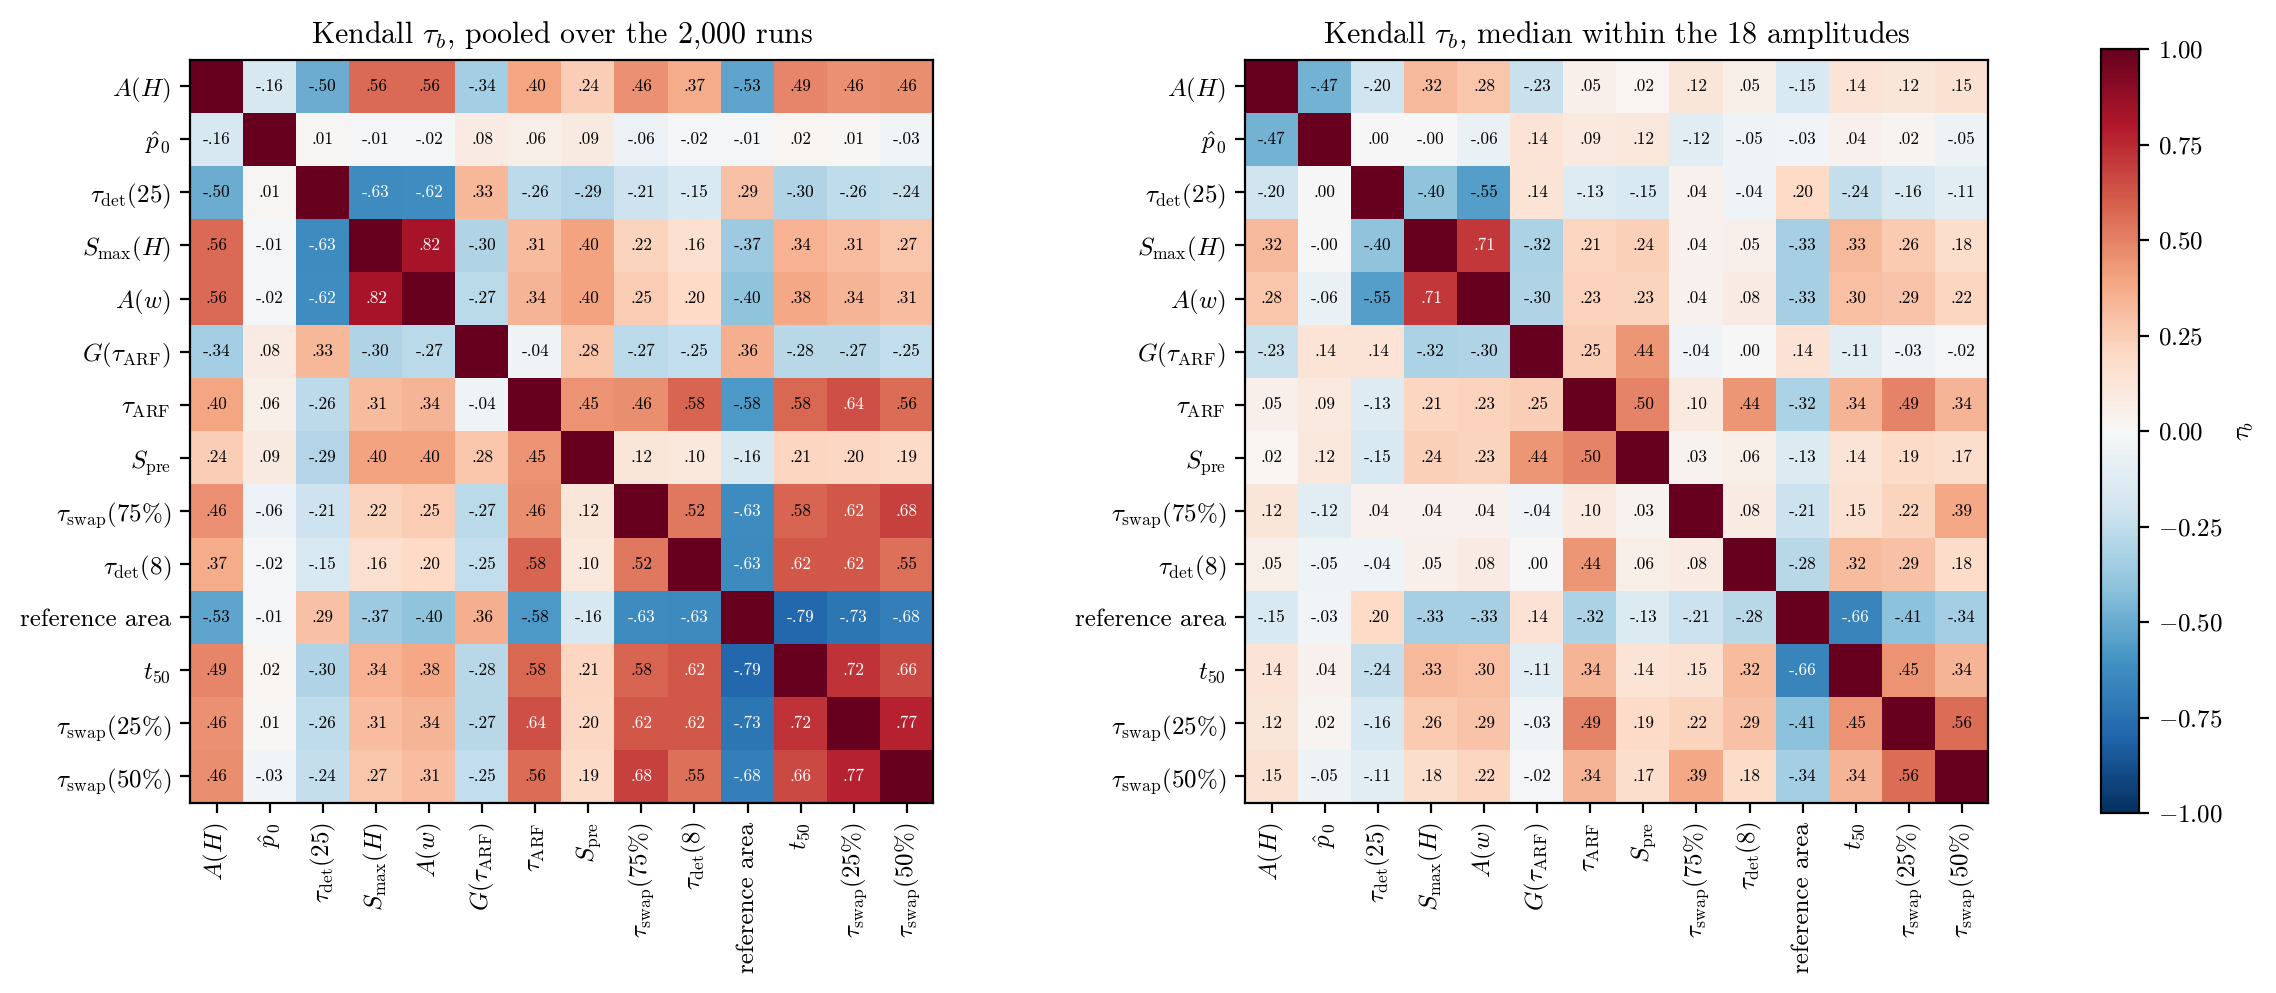
\includegraphics[width=0.86\textwidth]{Fig_QD_matrice_correlations_full.png}
  \end{center}
  \vspace{-0.5em}
  \small
  \begin{columns}[T,onlytextwidth]
    \begin{column}{0.32\textwidth}
      \textbf{Left, pooled:} almost everything agrees, because the drift size moves every
      indicator.
    \end{column}\hfill
    \begin{column}{0.32\textwidth}
      \textbf{Right, within a size:} two groups remain, \emph{evidence} ($0.71$) and
      \emph{repair}, weakly joined.
    \end{column}\hfill
    \begin{column}{0.32\textwidth}
      Best date against the analytic reference: \alert{3 trees replaced}, $0.45$, ahead of
      the first tree, $0.34$.
    \end{column}
  \end{columns}
  \note{To see all indicators at once, we crossed fourteen of them. The left panel pools all
    runs together: almost everything is strongly correlated with everything. That is an
    illusion, Simpson's paradox: the drift size moves every indicator, so pooling creates
    agreement. The right panel computes the same correlations within each drift size. Most of
    the agreement disappears, and two groups remain. One group measures evidence and damage:
    the detector's peak and the excess error over the transition agree strongly. The other
    group measures the repair. Between the two groups, links stay weak. We also compared the
    replacement dates with an analytic reference, the accuracy of the forest on the region
    whose label changed. The date at which three trees are replaced tracks it better than the
    first tree. This matrix is exploratory.}
\end{frame}

% =====================================================================
\section{III. Evidence vs threshold}
% =====================================================================

\begin{frame}{Part III --- Evidence against the threshold}
  \begin{center}\carte{3}\end{center}
  \note{The third part ties the first two together.}
\end{frame}

\begin{frame}{The race is decided before the repair}
  \begin{columns}[c,onlytextwidth]
    \begin{column}{0.52\textwidth}
      \centering
      \resizebox{\linewidth}{!}{\schemaidentite}\\
      {\scriptsize\color{gray} schematic}
    \end{column}\hfill
    \begin{column}{0.44\textwidth}
      A time counts observations; $\lambda$ counts \emph{excess errors}. Comparing them
      needs a rate that does not exist.
      \begin{block}{Race identity, on every run}
        \vspace{-0.4em}
        \[
          \tau_{\mathrm{det}} < \tau_{\mathrm{ARF}}
          \iff S_{\mathrm{pre}} \ge \lambda
        \]
        \vspace{-0.9em}
        \[
          S_{\mathrm{pre}} = \max_{t < \tau_{\mathrm{ARF}}} S_t
        \]
      \end{block}
      \small No rate, no averaging, no assumption on the trees. Checked on $2\,000$ runs out
      of $2\,000$ at three thresholds.
    \end{column}
  \end{columns}
  \note{Here is the key step. A repair time counts observations. A threshold counts excess
    errors. They are not in the same unit, and the paper bridges them with an average rate of
    errors per step. That rate does not exist: it falls as the forest repairs, and the
    detector forgets its evidence each time it hits zero. The exact statement is much
    simpler. Look at the statistic of the detector up to the first replacement, and take its
    highest point: we call it S pre. The detector arrives first if and only if S pre reaches
    the threshold. With a low threshold, it is reached before the repair; with a high one, it
    is not. This is exact on every run, it needs no rate, no averaging and no assumption on
    the trees, and we checked it on all two thousand runs.}
\end{frame}

\begin{frame}{The evidence before the repair sets the transition}
  \begin{columns}[c,onlytextwidth]
    \begin{column}{0.60\textwidth}
      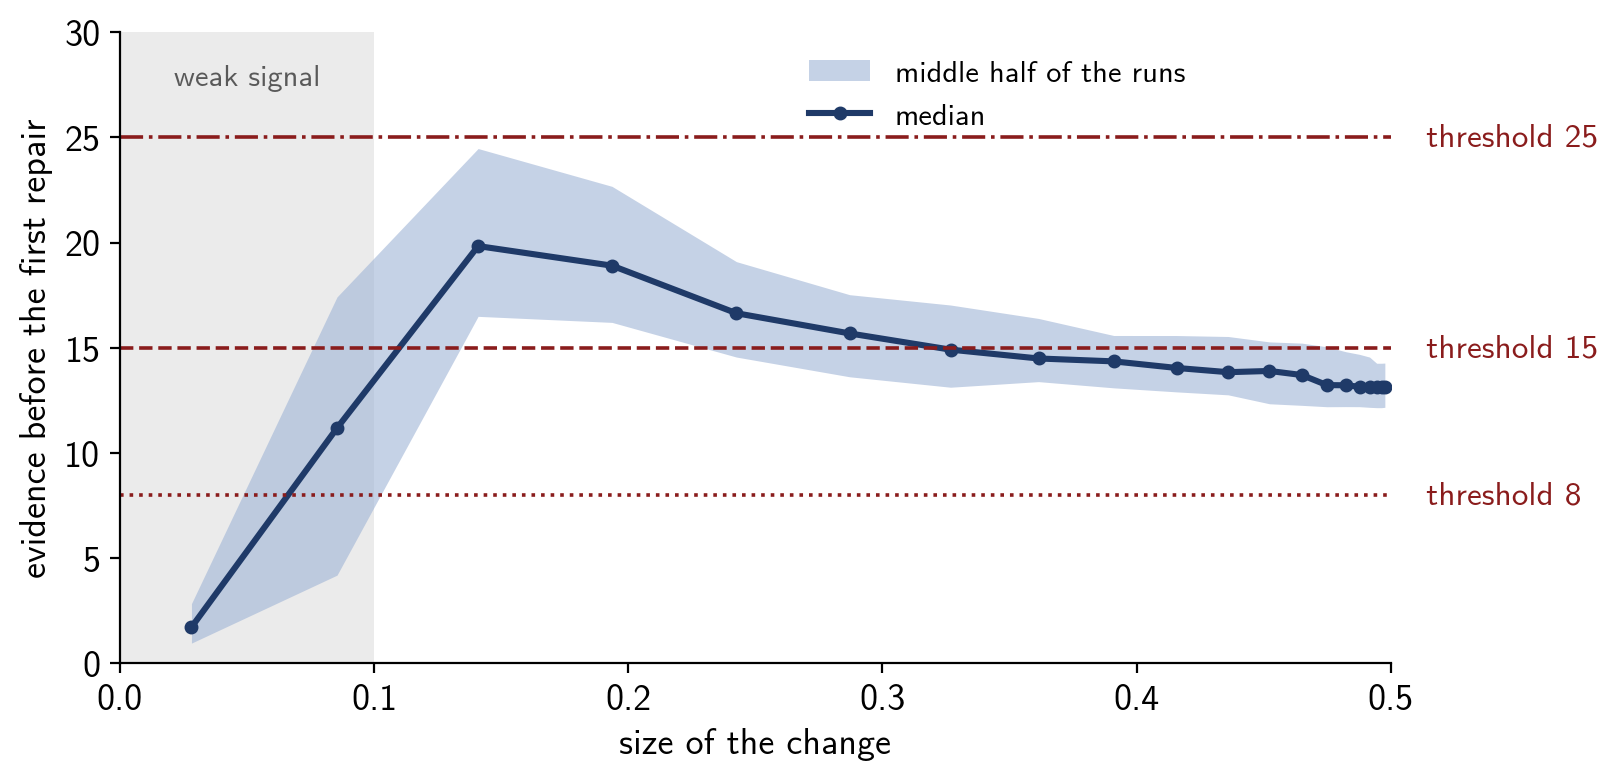
\includegraphics[width=\textwidth]{Fig_slide_spre.png}
    \end{column}\hfill
    \begin{column}{0.37\textwidth}
      \begin{itemize}
        \item Above the weak-signal zone, the median lies between \textbf{$13.1$ and $19.8$}:
              the transition the paper sees between $15$ and $25$, \alert{and leaves
              unexplained}.
        \item It \textbf{decreases} as the drift grows: at $\lambda = 15$ the detector wins
              $81\%$, then only $18\%$. That is the paradox.
      \end{itemize}
    \end{column}
  \end{columns}
  \note{So we measured S pre on every run. The dark line is the median by drift size, the band
    holds the middle half of the runs, and the red lines are thresholds. Above the weak-signal
    zone, the median sits between thirteen and twenty. A threshold below that level is reached
    before the repair in most runs; a threshold above it rarely is. That is exactly the
    transition the paper observes between fifteen and twenty-five, and leaves to future work.
    Now look at the shape. After the medium drifts, S pre decreases as the drift gets stronger,
    because the first replacement comes sooner. At a fixed threshold of fifteen, the detector
    wins eighty-one percent of the races on medium drifts, and only eighteen percent on the
    strongest ones. The paradox is this decreasing evidence, read against a fixed threshold. At
    the far left, the drift is too weak to accumulate anything: that is a different regime.}
\end{frame}

\begin{frame}{Stronger drifts leave no more evidence}
  \begin{columns}[c,onlytextwidth]
    \begin{column}{0.48\textwidth}
      \centering
      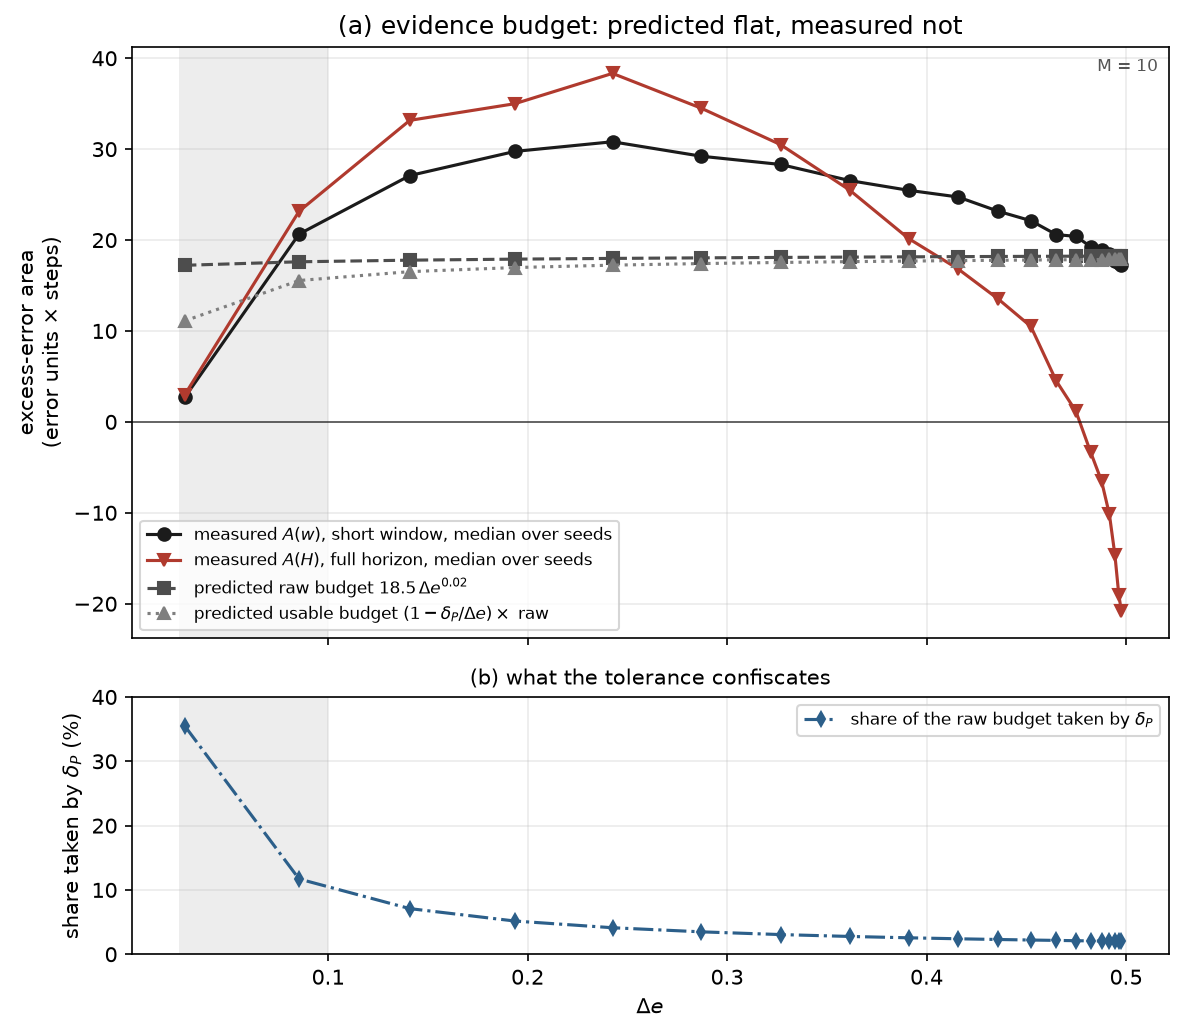
\includegraphics[height=0.66\textheight]{Fig_QC_budget_utilisable_full.png}
    \end{column}\hfill
    \begin{column}{0.46\textwidth}
      \begin{itemize}
        \item The paper's picture: an excess error $\Delta e$ over a window $\tau_{\mathrm{ARF}}$,
              so the area stays almost constant.
        \item Measured over the transition, the area varies by a factor of $1.8$ while the
              drift size varies by $5.8$: \alert{the compensation is real}.
        \item But the paper's rectangle misestimates it by up to $43\%$, and over the whole
              horizon the area turns negative at large drifts: the new task is easier.
      \end{itemize}
    \end{column}
  \end{columns}
  \note{Why doesn't a violent drift leave more evidence than a gentle one? The paper's picture
    is a rectangle: an excess error of height delta e, during a window equal to the repair
    time. Since the repair time shrinks like one over delta e, the area stays almost constant.
    We measured the area directly. Over the transition, it varies by a factor of less than two,
    while the drift size varies by almost six: the compensation is real. But the rectangle
    itself is wrong. It misestimates the area by up to forty-three percent, because the first
    replacement is not the width of the transient. And over the whole horizon, at large drifts,
    the area even becomes negative: after the change the task is easier than before, and the
    error settles below its old level. The evidence exists, it is roughly constant, but the
    paper's derivation of it does not hold.}
\end{frame}

\begin{frame}{Detecting is not winning}
  \begin{center}
    \begin{tabular}{@{}cccc@{}}
      \toprule
      threshold $\lambda$ & alarm fires & detector arrives first & false alarms, no drift \\
      \midrule
      $8$  & $95.3\%$ & $\mathbf{91.0\%}$ & $4.15\%$ \\
      $15$ & $92.9\%$ & $\mathbf{36.3\%}$ & $0.15\%$ \\
      $20$ & $66.2\%$ & $8.1\%$           & $0.00\%$ \\
      $25$ & $38.9\%$ & $2.5\%$           & $0.00\%$ \\
      \bottomrule
    \end{tabular}\\[0.3em]
    {\scriptsize\color{gray} $2\,000$ runs with drift and $2\,000$ without, over $2\,000$ steps}
  \end{center}
  \begin{itemize}
    \item At $\lambda = 15$ the alarm almost always fires, but mostly \emph{after} the repair.
    \item At $\lambda = 8$ the detector wins at an ordinary false-alarm cost: the paper's
          ``no threshold escapes'' does not hold on this bench.
    \item \textcolor{gray}{Not tested: the heteroscedastic streams where the paper places its
          false-alarm tension.}
  \end{itemize}
  \note{One practical consequence. Detecting a drift and winning the race are two different
    things. At threshold fifteen, the alarm fires on ninety-three percent of drifts, which
    looks excellent, but it arrives before the repair in only thirty-six percent of them.
    Most of these alarms come after the forest has already changed. At threshold eight, the
    detector wins ninety-one percent of the races, and it costs about four percent of false
    alarms over two thousand steps where nothing happens, which is an ordinary calibration
    level. So on this bench, one threshold does escape the blind spot, and the paper's claim
    that no threshold escapes has to be restricted. We did not test the financial streams
    with clustered volatility, where the paper places the false-alarm problem.}
\end{frame}

% =====================================================================
\section{Conclusion}
% =====================================================================

\begin{frame}{What changes in the paper}
  \small
  \begin{tabular}{@{}p{0.34\textwidth}p{0.43\textwidth}l@{}}
    \toprule
    The paper & Our result & \\
    \midrule
    races the repair against a constant & race identified, bounded, decided run by run & \textbf{made exact} \\
    independent trees, bias asserted & direction proven, cannot reverse & \textbf{proven} \\
    error back to normal at the first replacement & it comes back later; the rectangle fails & \textbf{corrected} \\
    first replacement as the repair date & earliest date, fires without drift & \textbf{qualified} \\
    transition between $15$ and $25$, unexplained & set by the evidence before the repair & \textbf{explained} \\
    no threshold escapes & $\lambda = 8$ does, on this bench & \textbf{restricted} \\
    \bottomrule
  \end{tabular}
  \vspace{0.6em}
  \begin{center}
    \alert{The phenomenon survives. What changes is its mechanism and its reach.}
  \end{center}
  \note{To sum up what our work changes in the paper. The race, which compared a random time
    with a constant, is made exact: identified, bounded, and decided run by run. The bias of
    the independence assumption was asserted; it is now proven, with its direction. The idea
    that the error is back to normal at the first replacement is corrected. The first
    replacement as a repair date is qualified: it is the earliest date and it fires without
    drift. The transition threshold, which the paper left unexplained, is explained by the
    evidence before the repair. And the claim that no threshold escapes is restricted to the
    settings the paper actually tested. The phenomenon survives all of this. What changes is
    its mechanism, and its reach.}
\end{frame}

\begin{frame}{An open question, and what we did not do}
  \begin{columns}[T,onlytextwidth]
    \begin{column}{0.50\textwidth}
      \begin{exampleblock}{Open: a reference for adaptation}
        Every indicator on the detector's side reads the \emph{error}, which mixes what the
        forest relearned with how hard the new task is. On analytic probes, the forest can
        relearn the changed region and lose a rare one, unseen by the error.
      \end{exampleblock}
    \end{column}\hfill
    \begin{column}{0.46\textwidth}
      \begin{block}{Not done}
        \small
        \begin{itemize}
          \item one forest size, one homoscedastic bench
          \item decision rule fixed during the analysis
          \item the independence bias has a sign, not a size
        \end{itemize}
      \end{block}
    \end{column}
  \end{columns}
  \note{We leave one question open. Every measure available to the detector reads the error,
    and the error mixes two things: what the forest has relearned, and how hard the new task
    is. Using analytic probes, points whose true label we know, we saw that the forest can
    relearn the region that changed while losing a rare region elsewhere, and the error does
    not see that loss. So what would a true reference for adaptation be? We do not have the
    answer. And to be honest about the limits: we studied one forest size on one simple
    bench, our decision rule was fixed during the analysis rather than before it, and we can
    give the sign of the independence bias but not its size.}
\end{frame}

\begin{frame}{Take-away}
  \begin{center}
    \small\alert{The blind spot is a budget of evidence, accumulated before the repair, set
    against a threshold.}
  \end{center}
  \vspace{-0.5em}
  \begin{center}\carte[0.71]{0}\end{center}
  \note{Back to the map. The blind spot is real, and it survives every correction. But it is
    not a race between two clocks. It is the evidence the forest lets through before its first
    repair, set against a fixed threshold. That single quantity explains when the detector
    wins, why the transition sits where it does, and why stronger drifts are missed more
    often. Thank you for your attention; we are happy to take your questions.}
\end{frame}

% =====================================================================
\appendix
\section*{Backup}
% =====================================================================

\begin{frame}{Backup --- Fréchet bounds}
  For integer-valued clocks with marginal CDFs $F_A$ and $F_D$, and \emph{any} coupling,
  \begin{align*}
    P_{\mathrm{miss}} &\ge \max\Big(0,\ \sup_{s} \big[F_A(s)-F_D(s)\big]\Big),\\
    P_{\mathrm{miss}} &\le \min\Big(1,\ \inf_{s} \big[F_A(s) + 1 - F_D(s+1)\big]\Big).
  \end{align*}
  \begin{itemize}
    \item Lower: Fréchet on $\{\tau_{\mathrm{ARF}} \le s < \tau_{\mathrm{det}}\} \subseteq \mathrm{Miss}$.
    \item Upper: $\mathrm{Miss} \subseteq \{\tau_{\mathrm{ARF}} \le s\} \cup \{\tau_{\mathrm{det}} > s+1\}$, then Boole.
    \item Toy case, both clocks uniform on $\{1,2\}$: the bounds $0$ and $0.5$ are both attained.
  \end{itemize}
\end{frame}

\begin{frame}{Backup --- Lindley's closed form and the certificate}
  With $X_t = e_t - \hat p_0 - \delta_P$ and $A(k,j) = \sum_{t=k+1}^{j} (e_t - \hat p_0)$,
  \[
    S_j = \max_{0 \le k \le j} \sum_{t=k+1}^{j} X_t,
    \qquad
    S_{\max}(H) = \max_{0 \le k \le j \le H} \big[A(k,j) - (j-k)\,\delta_P\big].
  \]
  \begin{itemize}
    \item Certificate: the alarm fires by $H$ iff some sub-window carries
          $A(k,j) \ge \lambda + (j-k)\,\delta_P$. The full window alone is only sufficient.
    \item Race identity: the same maximum, taken up to the first replacement, is $S_{\mathrm{pre}}$.
  \end{itemize}
\end{frame}

\begin{frame}{Backup --- Association protocol}
  \begin{itemize}
    \item Every coefficient is computed \textbf{within a drift size} ($100$ seeds), on the $18$
          sizes with $\Delta e \ge 0.10$: pooling measures the drift size, not the link.
    \item Kendall's $\tau_b$: reads on pairs, corrects for ties. Censored durations ranked last,
          licit because the horizon is common to all runs.
    \item Pearson undefined on censored values; Spearman handles their ties implicitly.
    \item Percentile bootstrap over seeds, $2\,000$ resamples; discernible if the interval
          excludes zero. Fixed during the analysis, not before: stated in the report.
    \item Complete cases instead of ranking censored runs last: no coefficient moves by more
          than $0.0403$.
  \end{itemize}
\end{frame}

\begin{frame}{Backup --- The drift-free control}
  \begin{center}
    \begin{tabular}{@{}lr@{}}
      \toprule
      On $2\,000$ runs with no change point & \\
      \midrule
      runs where at least one tree is replaced & $2\,000/2\,000$ \\
      first replacement, median & $95$ steps \\
      distinct trees renewed, median & $9/10$ \\
      forest entirely renewed & $28.7\%$ \\
      \midrule
      first replacement at the weakest drift, median & $118$ steps \\
      \bottomrule
    \end{tabular}
  \end{center}
\end{frame}

\end{document}
"
%
% Tracabilite : chaque chiffre vient du rapport ; controle par
%   verif_chiffres_tex.py ../../05_presentation/soutenance_20min.tex
% Figures : figures_slides.py --latex, figures_soutenance.py,
%   matrice_correlations.py, analyse_QCD.py (budget).
% =====================================================================

\documentclass[aspectratio=169,11pt]{beamer}

\usetheme{Madrid}
% Rouge de CentraleSupelec, pris dans le logo officiel (#B00739) ; logo
% CentraleSupelec / Universite Paris-Saclay sur la page de titre.
\definecolor{csRouge}{HTML}{B00739}
\usecolortheme[named=csRouge]{structure}
\setbeamercolor{alerted text}{fg=csRouge}
\setbeamersize{text margin left=1cm, text margin right=1cm}
\setbeamertemplate{navigation symbols}{}
\usepackage[english]{babel}
\usepackage{amsmath,amssymb}
\usepackage{graphicx}
\usepackage{booktabs}
\usepackage{tikz}
% soutenance_schemas.tex
% =====================================================================
% Schemas TikZ de `soutenance_20min.tex` : la carte des idees et le schema
% de l'identite de course.
%
% Fichier separe pour la meme raison que `point_encadrant_schemas.tex` :
% `verif_chiffres_tex.py` ramasserait les coordonnees TikZ comme des mesures.
% AUCUN chiffre de mesure ici ; les schemas sont stylises, sans donnees.
% =====================================================================

\usetikzlibrary{positioning, arrows.meta, calc}

\definecolor{mTheorie}{RGB}{31,58,104}
\definecolor{mDate}{RGB}{138,28,28}
\definecolor{mPreuve}{RGB}{38,92,58}
\definecolor{mEteint}{gray}{0.74}

% ---------------------------------------------------------------------
% \carte[hauteur]{k} : la carte des idees.
%   k = 0 : tout est actif (ouverture et conclusion)
%   k = 1, 2, 3 : seule la partie k est en couleur, le reste est grise
%   hauteur : fraction de \textheight (0.80 par defaut)
% Les fleches en pointille relient les parties ; elles sont commentees a
% l'oral plutot qu'etiquetees, faute de place entre les colonnes.
% ---------------------------------------------------------------------
\newcommand{\carte}[2][0.80]{%
  \colorlet{cUn}{mEteint}\colorlet{cDeux}{mEteint}\colorlet{cTrois}{mEteint}%
  \colorlet{tUn}{mEteint}\colorlet{tDeux}{mEteint}\colorlet{tTrois}{mEteint}%
  \ifnum#2=0 \colorlet{cUn}{mTheorie}\colorlet{cDeux}{mDate}\colorlet{cTrois}{mPreuve}%
    \colorlet{tUn}{black}\colorlet{tDeux}{black}\colorlet{tTrois}{black}\fi
  \ifnum#2=1 \colorlet{cUn}{mTheorie}\colorlet{tUn}{black}\fi
  \ifnum#2=2 \colorlet{cDeux}{mDate}\colorlet{tDeux}{black}\fi
  \ifnum#2=3 \colorlet{cTrois}{mPreuve}\colorlet{tTrois}{black}\fi
  \resizebox{!}{#1\textheight}{%
  \begin{tikzpicture}[
      font=\normalsize, align=center,
      boite/.style={draw, line width=1pt, rounded corners=3pt, inner sep=4pt,
                    text width=4.3cm, minimum height=1.05cm},
      un/.style={boite, draw=cUn, text=tUn},
      deux/.style={boite, draw=cDeux, text=tDeux},
      trois/.style={boite, draw=cTrois, text=tTrois},
      tete/.style={font=\bfseries\normalsize, text width=4.8cm},
      fl/.style={-{Stealth[length=2.4mm]}, line width=0.9pt},
      lien/.style={-{Stealth[length=2.4mm]}, line width=0.9pt, dashed},
    ]
    \node[boite, draw=black, fill=black!4, text width=12cm, minimum height=0.8cm] (P) at (5.6,0.15)
      {\textbf{The paper:} the stronger the drift, the faster the repair, the fewer the alarms};

    \node[tete, text=cUn]    (H1) at (0,-1.05)    {I.\ The race, formally};
    \node[tete, text=cDeux]  (H2) at (5.6,-1.05)  {II.\ The repair date};
    \node[tete, text=cTrois] (H3) at (11.2,-1.05) {III.\ Evidence vs threshold};
    \draw[fl, black!55] (P.south) -- ++(0,-0.25) -| (H1.north);
    \draw[fl, black!55] (P.south) -- (H2.north);
    \draw[fl, black!55] (P.south) -- ++(0,-0.25) -| (H3.north);

    \node[un] (A1) at (0,-2.1)  {The miss is well defined, its probability identified};
    \node[un] (A2) at (0,-3.45) {The blind spot holds whatever the dependence};
    \node[un] (B1) at (0,-4.8)  {Independent trees overstate the speed of repair};

    \node[deux] (C1) at (5.6,-2.1)  {The first replacement is the earliest date};
    \node[deux] (E1) at (5.6,-3.45) {It fires as fast when nothing changes};
    \node[deux] (D1) at (5.6,-4.8)  {When it fires, half the evidence is there};
    \node[deux] (D2) at (5.6,-6.15) {Indicators form two groups, weakly linked};

    \node[trois] (C2) at (11.2,-2.1)  {The alarm is a function of the error path};
    \node[trois] (K)  at (11.2,-3.45) {Detector first \emph{iff} it reaches $\lambda$ before the repair};
    \node[trois] (S)  at (11.2,-4.8)  {That evidence sets the transition and the paradox};
    \node[trois] (T)  at (11.2,-6.15) {Detecting is not winning};

    \node[boite, draw=black!55, text=black!80, dashed, text width=7cm, minimum height=0.8cm] (O) at (5.6,-7.45)
      {\textbf{Open:} a reference for adaptation itself};

    \draw[fl, cUn]    (A1) -- (A2);
    \draw[fl, cDeux]  (C1) -- (E1);
    \draw[fl, cDeux]  (E1) -- (D1);
    \draw[fl, cDeux]  (D1) -- (D2);
    \draw[fl, cTrois] (C2) -- (K);
    \draw[fl, cTrois] (K) -- (S);
    \draw[fl, cTrois] (S) -- (T);
    \draw[lien, black!55] (B1.east) -- (D1.west);
    \draw[lien, black!55] (D1.east) -- (S.west);
    \draw[lien, black!55] (D2.south) -- (O.north);
  \end{tikzpicture}}%
}

% ---------------------------------------------------------------------
% \schemaidentite : la pile S_t, le premier remplacement, deux seuils.
% Stylise, sans donnees.
% ---------------------------------------------------------------------
\newcommand{\schemaidentite}{%
  \begin{tikzpicture}[x=1cm, y=1cm, font=\small]
    \draw[-{Stealth}, line width=0.7pt] (0,0) -- (7.2,0);
    \node[below left] at (7.2,-0.05) {time};
    \draw[-{Stealth}, line width=0.7pt] (0,0) -- (0,3.7);
    \node[rotate=90, above] at (-0.05,1.85) {detector statistic $S_t$};
    \draw[line width=1.4pt, mTheorie]
      (0,0) .. controls (0.8,0.6) and (1.6,1.9) .. (2.4,2.25)
            .. controls (3.0,2.5) and (3.4,2.55) .. (3.9,2.4)
            .. controls (4.8,2.0) and (5.8,1.0) .. (7.0,0.3);
    \draw[dashed, mDate, line width=1pt] (2.8,0) -- (2.8,3.4);
    \node[above, text=mDate] at (2.8,3.4) {first replacement};
    \fill[mTheorie] (2.8,2.38) circle (2.3pt);
    \node[above left, text=mTheorie] at (2.75,2.4) {$S_{\mathrm{pre}}$};
    \draw[mPreuve, line width=1pt] (0,1.5) -- (7.0,1.5);
    \node[above left, text=mPreuve] at (7.0,1.5) {low $\lambda$: reached before};
    \draw[mDate, line width=1pt, dash dot] (0,3.0) -- (7.0,3.0);
    \node[above left, text=mDate] at (7.0,3.0) {high $\lambda$: not reached};
  \end{tikzpicture}%
}

\titlegraphic{
\includegraphics[height=1.7cm]{Logo_CS_Paris_Saclay.png}}
\ifdefined\NOTESSEULES\setbeameroption{show only notes}\fi
\graphicspath{{../04_experimentations/resultats_R2/resultats/figures/slides_latex/}{../04_experimentations/resultats_R2/resultats/figures/}}

\setbeamerfont{author}{size=\small}
\setbeamerfont{institute}{size=\scriptsize}

\title[The Blind Spot Paradox]{The Blind Spot Paradox}
\subtitle{Formalizing the race and measuring the adaptation}
\author[Boyer, Gouillou, Fonvielle, Petit-Tichanné]{Alexandre Boyer \and Melaine Gouillou \and Salomé Fonvielle \and Ulysse Petit-Tichanné}
\institute[CS]{Research Track, Topic 39, CentraleSupélec. Supervisor: Raphaël Minato}
\date{16 September 2026}

\begin{document}

\maketitle
\note{Good afternoon. Our subject is the blind spot paradox: a model that repairs
  itself can destroy the very evidence its own monitor needs. In the next twenty
  minutes we will present what we formalized, what we measured, and the single
  reading that ties the two together.}

% =====================================================================
\section{The problem}
% =====================================================================

\begin{frame}{Concept drift: the rule changes, the data does not}
  \vspace{-0.6em}
  \[
    \underbrace{P(X)}_{\text{the data}}\ \text{unchanged}
    \qquad\qquad
    \underbrace{P(Y \mid X)}_{\text{the rule}}\ \text{changes}
  \]
  \vspace{-0.9em}
  \begin{center}
    
\includegraphics[height=0.50\textheight]{Fig_slide_drift.png}
  \end{center}
  \begin{center}
    A model trained before the change is now \alert{wrong on the shaded band}.
  \end{center}
  \note{A classifier learns a rule from data. In a data stream, that rule can change
    while the inputs keep exactly the same distribution. This is concept drift: P of X
    does not move, P of Y given X does. It is the normal situation for a financial
    signal, where the same inputs stop meaning the same thing. In the bench we use,
    points in the plane are separated by a line. At the change, the line moves. Every
    point in the shaded band switches label, so a model trained before the change keeps
    predicting confidently, and is now wrong on that band. The size of the band is the
    size of the drift, written delta e.}
\end{frame}

\begin{frame}{Two defences that run at the same time}
  \begin{columns}[T,onlytextwidth]
    \begin{column}{0.49\textwidth}
      \centering
      \textbf{The model repairs itself}\\[0.3em]
      
\includegraphics[width=\textwidth]{Fig_slide_foret.png}\\[0.2em]
      \small Adaptive Random Forest: ten trees, each replaced when its own error rises.
    \end{column}\hfill
    \begin{column}{0.49\textwidth}
      \centering
      \textbf{A monitor raises the alarm}\\[0.3em]
      
\includegraphics[width=\textwidth]{Fig_slide_watchdog.png}\\[0.2em]
      \small Each error adds to a statistic $S_t$; the alarm fires when it crosses $\lambda$.
    \end{column}
  \end{columns}
  \note{Two defences are deployed together. The first one lives inside the model. The
    Adaptive Random Forest is made of ten decision trees that vote. Each tree watches its
    own error with a small detector, and when that error rises, the tree is replaced by a
    fresh one. The forest repairs itself locally, without asking anyone. The second defence
    sits outside. A cumulative detector, a Page-Hinkley test, watches the error of the
    whole forest. Every error pushes a statistic up by almost one, every correct answer
    pulls it down a little, never below zero. When the statistic crosses a threshold
    lambda, the alarm fires, and that alarm is the only thing a human operator sees.}
\end{frame}

\begin{frame}{The paradox, and what the reviewers asked}
  \begin{columns}[c,onlytextwidth]
    \begin{column}{0.50\textwidth}
      \centering
      
\includegraphics[width=\textwidth]{Fig_slide_mecanisme.png}\\
      {\scriptsize\color{gray} schematic}
    \end{column}\hfill
    \begin{column}{0.46\textwidth}
      \begin{block}{The paper's claim}
        The stronger the drift, the faster the repair, and the \alert{fewer} alarms.
      \end{block}
      \begin{alertblock}{Two corrections requested}
        \begin{enumerate}
          \item It races a random repair time against a \emph{constant}, and assumes the
                trees independent.
          \item It dates the repair at the \emph{first} tree replaced, without showing
                that this date means anything.
        \end{enumerate}
      \end{alertblock}
    \end{column}
  \end{columns}
  \note{When both defences run together, something unexpected happens. The drift starts,
    errors pile up in the detector, but the forest replaces trees, the errors stop, and the
    pile drains before it reaches the threshold. The paper we study calls this the blind
    spot paradox: the stronger the drift, the faster the forest repairs itself, and the
    fewer alarms the operator gets. The paper was reviewed, and two corrections were
    requested. First, it compares a random repair time with a constant detection time, and
    it assumes the ten trees are independent without proving it. Second, it dates the repair
    at the moment the first tree is replaced, without showing that this moment has anything
    to do with the error disappearing. These two corrections are where our work starts.}
\end{frame}

\begin{frame}{Our reading, in one map}
  \begin{center}
    \small\alert{The blind spot is not a race between two clocks,
    but a budget of evidence set against a threshold.}
  \end{center}
  \vspace{-0.5em}
  \begin{center}
    \carte[0.71]{0}
  \end{center}
  \note{Here is the whole talk on one map. At the top, the claim of the paper. The first
    column formalizes the race: we define the blind spot properly, we compute its
    probability, and we show that assuming independent trees makes the paper optimistic
    about the repair. The second column asks what the repair date really measures: it is
    the earliest possible date, it fires even when nothing changes, and when it fires most
    of the evidence is already there. The third column ties both together: the detector wins
    exactly when its evidence reaches the threshold before the repair, and that evidence
    explains both the transition and the paradox. The dashed arrows are the links between
    columns, and the box at the bottom is the question we leave open. Our one-sentence
    reading: the blind spot is not a race between two clocks, it is a budget of evidence set
    against a threshold.}
\end{frame}

% =====================================================================
\section{I. The race}
% =====================================================================

\begin{frame}{Part I --- The race, formally}
  \begin{center}\carte{1}\end{center}
  \note{Let us start with the theory: how to state the race without cheating.}
\end{frame}

\begin{frame}{The race is well posed, and its probability identified}
  \begin{columns}[T,onlytextwidth]
    \begin{column}{0.46\textwidth}
      \begin{block}{One definition, no ad hoc rule}
        \[
          \mathrm{Miss} := \{\tau_{\mathrm{ARF}} < \tau_{\mathrm{det}}\}
        \]
        \vspace{-0.6em}
        {\small strict inequality; the alarm may never come}
        \begin{itemize}
          \item a tie goes to the detector
          \item a silent repair, with no alarm ever, \alert{is} a miss
          \item if neither acts, it is not
        \end{itemize}
      \end{block}
    \end{column}\hfill
    \begin{column}{0.50\textwidth}
      \begin{exampleblock}{What the campaign allows}
        The forest always replaces a tree within the horizon, so no run is left
        undecided: $P_{\mathrm{miss}}$ is \textbf{identified}.\\[0.3em]
        \centering
        \begin{tabular}{@{}lccc@{}}
          $\lambda$ & $8$ & $25$ & $50$ \\
          $P_{\mathrm{miss}}$ & $0.0905$ & $0.9715$ & $1.0000$
        \end{tabular}
      \end{exampleblock}
      \begin{alertblock}{Without any dependence assumption}
        From the marginal laws alone, the blind spot at the weakest drift is at least
        $0.91$ at $\lambda = 8$.
      \end{alertblock}
    \end{column}
  \end{columns}
  \note{The paper says there is a blind spot when the forest repairs before the alarm, but
    it quietly sets aside the runs where the alarm never comes. Those are exactly the runs
    where the detector fails most. So we define the event on the complete race, with one
    definition and no extra rule. A tie counts for the detector, because the operator is
    warned at the right moment. A silent repair, where the alarm never comes, is a miss, and
    in fact the purest one. A run where neither mechanism acts is not a miss, because there
    was nothing to erase. Then comes the problem of the finite horizon: some runs could be
    undecided. On our campaign they are not, because the forest always acts within the
    horizon, so the miss probability is identified exactly: nine percent at threshold eight,
    ninety-seven at twenty-five, one hundred at fifty. And with Fréchet bounds, which use the
    two marginal laws and assume nothing on how the clocks are coupled, the blind spot at the
    weakest drift is already forced above ninety percent.}
\end{frame}

\begin{frame}{Trees share a stream: the paper is optimistic}
  \begin{enumerate}
    \item \textbf{Given the stream}, what separates two trees is their own random draws:
          the trees are independent \emph{conditionally}.
    \item \textbf{Averaging over streams}, convexity gives the direction:
          \[
            P(\tau_{\mathrm{ARF}} \le s) \;\le\; 1 - \big(1 - F(s)\big)^M
          \]
          \alert{The independence formula overstates the speed of the repair.}
    \item \textbf{Consequence}: the paper's critical ensemble size becomes a conservative
          ceiling; its verdict does not change.
    \item \textbf{No coupling reverses the sign}: sharing a stream can only make trees fail
          together, since the covariance equals a variance.
  \end{enumerate}
  \note{The second shortcut is independence. The ten trees learn from the same stream, so
    they cannot be independent. But the question is at which level. Once the stream is
    fixed, what distinguishes one tree from another is only its own randomness, the random
    weights of online bagging. At that level, given the stream, the trees are independent.
    When we average over streams, Jensen's inequality gives a clear direction: the
    probability that the forest has already repaired itself is at most what the independence
    formula predicts. So the paper makes the forest look faster than it is, and overestimates
    the blind spot. Its critical ensemble size is not wrong, it becomes a conservative
    ceiling, and the paper's own verdict does not change. Could dependence go the other way?
    No: the covariance between two trees equals a variance, so it is never negative.}
\end{frame}

% =====================================================================
\section{II. The repair date}
% =====================================================================

\begin{frame}{Part II --- What the repair date measures}
  \begin{center}\carte{2}\end{center}
  \note{Now the second correction: the date the paper uses for the repair.}
\end{frame}

\begin{frame}{How we measured}
  \begin{columns}[T,onlytextwidth]
    \begin{column}{0.48\textwidth}
      \begin{block}{The campaign}
        \begin{itemize}
          \item the paper's bench, rerun: $20$ drift sizes $\times$ $100$ seeds,
                $2\,000$ steps after the change
          \item $2\,000$ more runs with no change at all
          \item only the error and the replacement events are recorded; every threshold is
                replayed offline
        \end{itemize}
      \end{block}
    \end{column}\hfill
    \begin{column}{0.48\textwidth}
      \begin{block}{Reading an association}
        \begin{itemize}
          \item always \alert{within one drift size}: pooling measures the drift size, not
                the link
          \item Kendall's rank correlation, with bootstrap intervals over the seeds
          \item steps added after seeing the data are flagged as exploratory
        \end{itemize}
      \end{block}
    \end{column}
  \end{columns}
  \note{A word on how we measured, without the implementation details. We reran the bench
    of the paper on twenty drift sizes, with one hundred seeds each, and we observe two
    thousand steps after the change. We added two thousand runs where nothing changes at
    all, as a control. The simulation records only two things: the error at each step and
    the moments when trees are replaced. Everything else, including the detector at any
    threshold, is recomputed offline, so one campaign replaces many. When we correlate two
    quantities, we always do it within one drift size. The drift size moves every indicator
    at once, so a correlation pooled over sizes mostly measures the size itself. We use
    Kendall's rank correlation with bootstrap intervals, and we flag the steps we added
    after looking at the data.}
\end{frame}

\begin{frame}{The first replacement is the earliest possible date}
  \begin{center}
    
\includegraphics[width=0.90\textwidth]{Fig_slide_deux_horloges.png}
  \end{center}
  \vspace{-0.3em}
  \begin{itemize}
    \item On every run, the first replacement comes before any other quota of renewed
          trees. Three quarters of the forest are renewed \textbf{$6.0$ to $14.3$ times later}.
    \item \alert{With no drift at all}, the first replacement comes after $95$ steps in
          median, against $118$ on the weakest drift.
  \end{itemize}
  \note{The paper dates the repair at the first replaced tree. By construction, that is the
    earliest of all possible dates: the moment when three trees, or half, or three quarters
    of the forest are replaced, always comes later, on every run. The only question is how
    much later. On this medium drift, the first tree goes after eighty-six observations, and
    three quarters of the forest after more than twelve hundred. Over the grid, three
    quarters of the forest are renewed six to fourteen times later than the first tree. And
    there is a more worrying fact. On the two thousand runs with no change at all, the forest
    still replaces its first tree, after ninety-five steps in median. On the weakest real
    drift, it takes one hundred and eighteen. So at low drift, this date cannot tell a real
    change from noise.}
\end{frame}

\begin{frame}{When the first tree goes, most of the evidence is already there}
  \begin{columns}[T,onlytextwidth]
    \begin{column}{0.36\textwidth}
      \begin{block}{Evidence at the first replacement}
        \centering
        {\Large $49\%$ to $76\%$}\\[0.2em]
        \small of the detector's final peak, on the $18$ drift sizes studied
      \end{block}
    \end{column}\hfill
    \begin{column}{0.60\textwidth}
      \begin{block}{Does the date track anything, within a drift size?}
        \small
        \begin{tabular}{@{}lcc@{}}
          \toprule
          compared with & median link & sizes \\
          \midrule
          detector peak & $0.21$ & $15/18$ \\
          excess error, whole horizon & none & $0/18$ \\
          excess error, transition only & $0.23$ & $13/18$ \\
          \bottomrule
        \end{tabular}
      \end{block}
    \end{column}
  \end{columns}
  \vspace{0.8em}
  \begin{center}
    \small The null over the whole horizon is mostly noise: \alert{half} of that area's
    variance comes from the estimated baseline, multiplied by the horizon.
  \end{center}
  \note{Is the first replacement at least the end of the transient? No. When the first tree
    is replaced, the detector already holds between half and three quarters of all the
    evidence it will ever accumulate. The replacement is in the middle of the story, not at
    its end. Then we asked whether this date tracks anything, always within a drift size.
    With the peak of the detector, there is a weak but real link, visible on fifteen drift
    sizes out of eighteen. With the excess error over the whole horizon, there is no link at
    all. But we found out why: that area adds up two thousand steps, so any error on the
    baseline is multiplied by two thousand, and half of its variance is just that noise. If
    we keep only the transition, the link comes back, weak but real, on thirteen sizes out of
    eighteen. This last step is exploratory.}
\end{frame}

\begin{frame}{Unexpected: pooling manufactures agreement}
  \begin{center}
    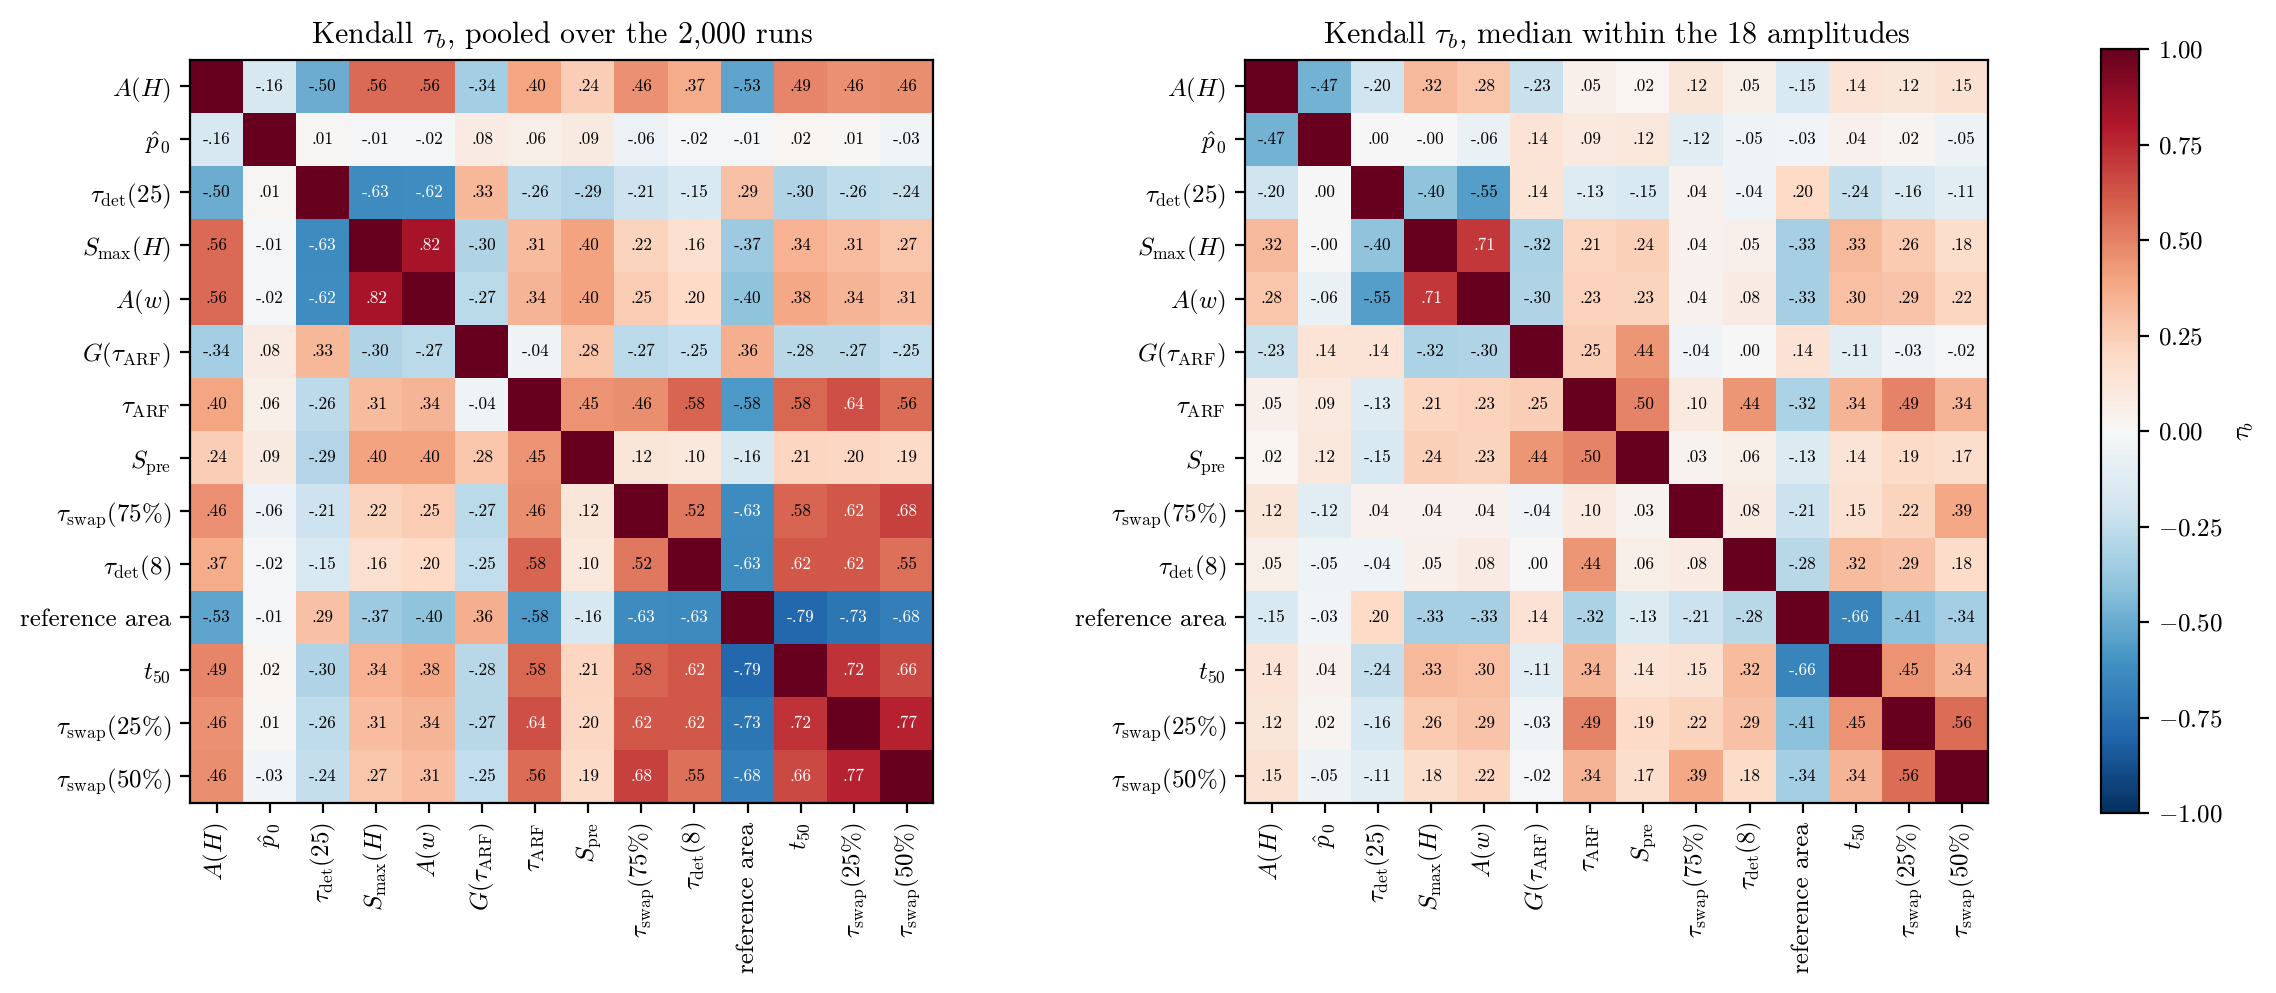
\includegraphics[width=0.86\textwidth]{Fig_QD_matrice_correlations_full.png}
  \end{center}
  \vspace{-0.5em}
  \small
  \begin{columns}[T,onlytextwidth]
    \begin{column}{0.32\textwidth}
      \textbf{Left, pooled:} almost everything agrees, because the drift size moves every
      indicator.
    \end{column}\hfill
    \begin{column}{0.32\textwidth}
      \textbf{Right, within a size:} two groups remain, \emph{evidence} ($0.71$) and
      \emph{repair}, weakly joined.
    \end{column}\hfill
    \begin{column}{0.32\textwidth}
      Best date against the analytic reference: \alert{3 trees replaced}, $0.45$, ahead of
      the first tree, $0.34$.
    \end{column}
  \end{columns}
  \note{To see all indicators at once, we crossed fourteen of them. The left panel pools all
    runs together: almost everything is strongly correlated with everything. That is an
    illusion, Simpson's paradox: the drift size moves every indicator, so pooling creates
    agreement. The right panel computes the same correlations within each drift size. Most of
    the agreement disappears, and two groups remain. One group measures evidence and damage:
    the detector's peak and the excess error over the transition agree strongly. The other
    group measures the repair. Between the two groups, links stay weak. We also compared the
    replacement dates with an analytic reference, the accuracy of the forest on the region
    whose label changed. The date at which three trees are replaced tracks it better than the
    first tree. This matrix is exploratory.}
\end{frame}

% =====================================================================
\section{III. Evidence vs threshold}
% =====================================================================

\begin{frame}{Part III --- Evidence against the threshold}
  \begin{center}\carte{3}\end{center}
  \note{The third part ties the first two together.}
\end{frame}

\begin{frame}{The race is decided before the repair}
  \begin{columns}[c,onlytextwidth]
    \begin{column}{0.52\textwidth}
      \centering
      \resizebox{\linewidth}{!}{\schemaidentite}\\
      {\scriptsize\color{gray} schematic}
    \end{column}\hfill
    \begin{column}{0.44\textwidth}
      A time counts observations; $\lambda$ counts \emph{excess errors}. Comparing them
      needs a rate that does not exist.
      \begin{block}{Race identity, on every run}
        \vspace{-0.4em}
        \[
          \tau_{\mathrm{det}} < \tau_{\mathrm{ARF}}
          \iff S_{\mathrm{pre}} \ge \lambda
        \]
        \vspace{-0.9em}
        \[
          S_{\mathrm{pre}} = \max_{t < \tau_{\mathrm{ARF}}} S_t
        \]
      \end{block}
      \small No rate, no averaging, no assumption on the trees. Checked on $2\,000$ runs out
      of $2\,000$ at three thresholds.
    \end{column}
  \end{columns}
  \note{Here is the key step. A repair time counts observations. A threshold counts excess
    errors. They are not in the same unit, and the paper bridges them with an average rate of
    errors per step. That rate does not exist: it falls as the forest repairs, and the
    detector forgets its evidence each time it hits zero. The exact statement is much
    simpler. Look at the statistic of the detector up to the first replacement, and take its
    highest point: we call it S pre. The detector arrives first if and only if S pre reaches
    the threshold. With a low threshold, it is reached before the repair; with a high one, it
    is not. This is exact on every run, it needs no rate, no averaging and no assumption on
    the trees, and we checked it on all two thousand runs.}
\end{frame}

\begin{frame}{The evidence before the repair sets the transition}
  \begin{columns}[c,onlytextwidth]
    \begin{column}{0.60\textwidth}
      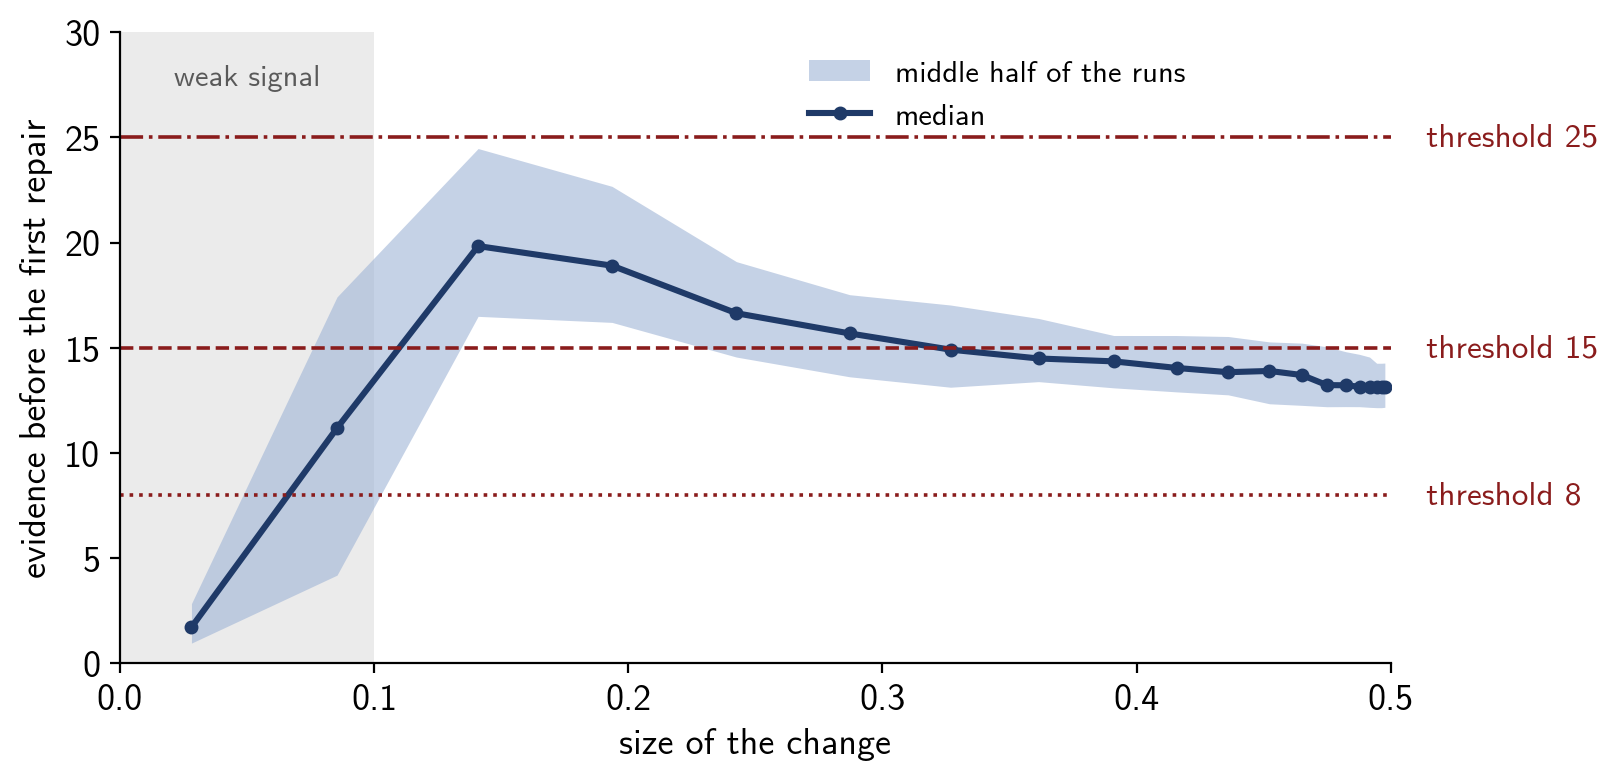
\includegraphics[width=\textwidth]{Fig_slide_spre.png}
    \end{column}\hfill
    \begin{column}{0.37\textwidth}
      \begin{itemize}
        \item Above the weak-signal zone, the median lies between \textbf{$13.1$ and $19.8$}:
              the transition the paper sees between $15$ and $25$, \alert{and leaves
              unexplained}.
        \item It \textbf{decreases} as the drift grows: at $\lambda = 15$ the detector wins
              $81\%$, then only $18\%$. That is the paradox.
      \end{itemize}
    \end{column}
  \end{columns}
  \note{So we measured S pre on every run. The dark line is the median by drift size, the band
    holds the middle half of the runs, and the red lines are thresholds. Above the weak-signal
    zone, the median sits between thirteen and twenty. A threshold below that level is reached
    before the repair in most runs; a threshold above it rarely is. That is exactly the
    transition the paper observes between fifteen and twenty-five, and leaves to future work.
    Now look at the shape. After the medium drifts, S pre decreases as the drift gets stronger,
    because the first replacement comes sooner. At a fixed threshold of fifteen, the detector
    wins eighty-one percent of the races on medium drifts, and only eighteen percent on the
    strongest ones. The paradox is this decreasing evidence, read against a fixed threshold. At
    the far left, the drift is too weak to accumulate anything: that is a different regime.}
\end{frame}

\begin{frame}{Stronger drifts leave no more evidence}
  \begin{columns}[c,onlytextwidth]
    \begin{column}{0.48\textwidth}
      \centering
      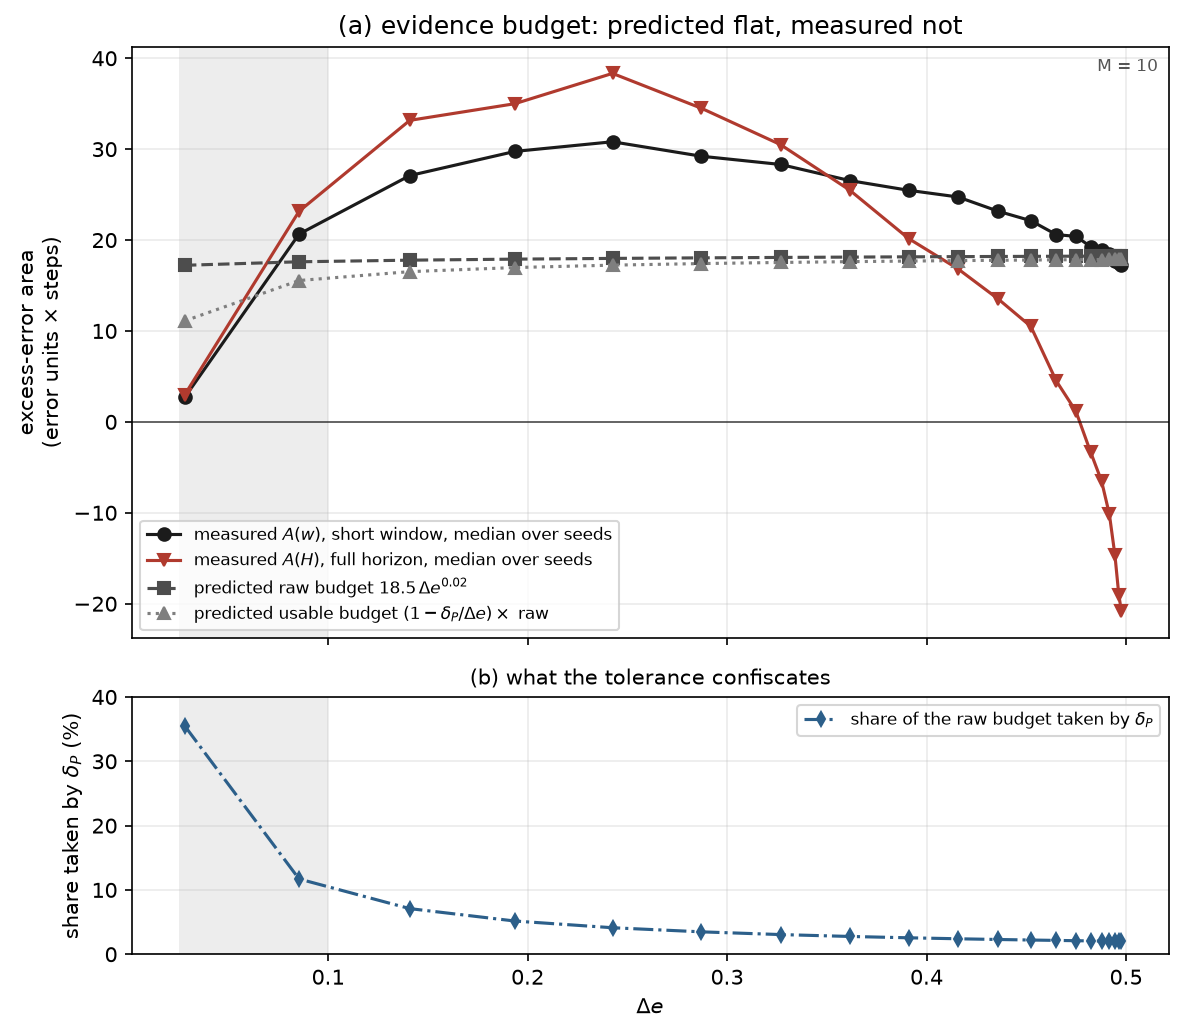
\includegraphics[height=0.66\textheight]{Fig_QC_budget_utilisable_full.png}
    \end{column}\hfill
    \begin{column}{0.46\textwidth}
      \begin{itemize}
        \item The paper's picture: an excess error $\Delta e$ over a window $\tau_{\mathrm{ARF}}$,
              so the area stays almost constant.
        \item Measured over the transition, the area varies by a factor of $1.8$ while the
              drift size varies by $5.8$: \alert{the compensation is real}.
        \item But the paper's rectangle misestimates it by up to $43\%$, and over the whole
              horizon the area turns negative at large drifts: the new task is easier.
      \end{itemize}
    \end{column}
  \end{columns}
  \note{Why doesn't a violent drift leave more evidence than a gentle one? The paper's picture
    is a rectangle: an excess error of height delta e, during a window equal to the repair
    time. Since the repair time shrinks like one over delta e, the area stays almost constant.
    We measured the area directly. Over the transition, it varies by a factor of less than two,
    while the drift size varies by almost six: the compensation is real. But the rectangle
    itself is wrong. It misestimates the area by up to forty-three percent, because the first
    replacement is not the width of the transient. And over the whole horizon, at large drifts,
    the area even becomes negative: after the change the task is easier than before, and the
    error settles below its old level. The evidence exists, it is roughly constant, but the
    paper's derivation of it does not hold.}
\end{frame}

\begin{frame}{Detecting is not winning}
  \begin{center}
    \begin{tabular}{@{}cccc@{}}
      \toprule
      threshold $\lambda$ & alarm fires & detector arrives first & false alarms, no drift \\
      \midrule
      $8$  & $95.3\%$ & $\mathbf{91.0\%}$ & $4.15\%$ \\
      $15$ & $92.9\%$ & $\mathbf{36.3\%}$ & $0.15\%$ \\
      $20$ & $66.2\%$ & $8.1\%$           & $0.00\%$ \\
      $25$ & $38.9\%$ & $2.5\%$           & $0.00\%$ \\
      \bottomrule
    \end{tabular}\\[0.3em]
    {\scriptsize\color{gray} $2\,000$ runs with drift and $2\,000$ without, over $2\,000$ steps}
  \end{center}
  \begin{itemize}
    \item At $\lambda = 15$ the alarm almost always fires, but mostly \emph{after} the repair.
    \item At $\lambda = 8$ the detector wins at an ordinary false-alarm cost: the paper's
          ``no threshold escapes'' does not hold on this bench.
    \item \textcolor{gray}{Not tested: the heteroscedastic streams where the paper places its
          false-alarm tension.}
  \end{itemize}
  \note{One practical consequence. Detecting a drift and winning the race are two different
    things. At threshold fifteen, the alarm fires on ninety-three percent of drifts, which
    looks excellent, but it arrives before the repair in only thirty-six percent of them.
    Most of these alarms come after the forest has already changed. At threshold eight, the
    detector wins ninety-one percent of the races, and it costs about four percent of false
    alarms over two thousand steps where nothing happens, which is an ordinary calibration
    level. So on this bench, one threshold does escape the blind spot, and the paper's claim
    that no threshold escapes has to be restricted. We did not test the financial streams
    with clustered volatility, where the paper places the false-alarm problem.}
\end{frame}

% =====================================================================
\section{Conclusion}
% =====================================================================

\begin{frame}{What changes in the paper}
  \small
  \begin{tabular}{@{}p{0.34\textwidth}p{0.43\textwidth}l@{}}
    \toprule
    The paper & Our result & \\
    \midrule
    races the repair against a constant & race identified, bounded, decided run by run & \textbf{made exact} \\
    independent trees, bias asserted & direction proven, cannot reverse & \textbf{proven} \\
    error back to normal at the first replacement & it comes back later; the rectangle fails & \textbf{corrected} \\
    first replacement as the repair date & earliest date, fires without drift & \textbf{qualified} \\
    transition between $15$ and $25$, unexplained & set by the evidence before the repair & \textbf{explained} \\
    no threshold escapes & $\lambda = 8$ does, on this bench & \textbf{restricted} \\
    \bottomrule
  \end{tabular}
  \vspace{0.6em}
  \begin{center}
    \alert{The phenomenon survives. What changes is its mechanism and its reach.}
  \end{center}
  \note{To sum up what our work changes in the paper. The race, which compared a random time
    with a constant, is made exact: identified, bounded, and decided run by run. The bias of
    the independence assumption was asserted; it is now proven, with its direction. The idea
    that the error is back to normal at the first replacement is corrected. The first
    replacement as a repair date is qualified: it is the earliest date and it fires without
    drift. The transition threshold, which the paper left unexplained, is explained by the
    evidence before the repair. And the claim that no threshold escapes is restricted to the
    settings the paper actually tested. The phenomenon survives all of this. What changes is
    its mechanism, and its reach.}
\end{frame}

\begin{frame}{An open question, and what we did not do}
  \begin{columns}[T,onlytextwidth]
    \begin{column}{0.50\textwidth}
      \begin{exampleblock}{Open: a reference for adaptation}
        Every indicator on the detector's side reads the \emph{error}, which mixes what the
        forest relearned with how hard the new task is. On analytic probes, the forest can
        relearn the changed region and lose a rare one, unseen by the error.
      \end{exampleblock}
    \end{column}\hfill
    \begin{column}{0.46\textwidth}
      \begin{block}{Not done}
        \small
        \begin{itemize}
          \item one forest size, one homoscedastic bench
          \item decision rule fixed during the analysis
          \item the independence bias has a sign, not a size
        \end{itemize}
      \end{block}
    \end{column}
  \end{columns}
  \note{We leave one question open. Every measure available to the detector reads the error,
    and the error mixes two things: what the forest has relearned, and how hard the new task
    is. Using analytic probes, points whose true label we know, we saw that the forest can
    relearn the region that changed while losing a rare region elsewhere, and the error does
    not see that loss. So what would a true reference for adaptation be? We do not have the
    answer. And to be honest about the limits: we studied one forest size on one simple
    bench, our decision rule was fixed during the analysis rather than before it, and we can
    give the sign of the independence bias but not its size.}
\end{frame}

\begin{frame}{Take-away}
  \begin{center}
    \small\alert{The blind spot is a budget of evidence, accumulated before the repair, set
    against a threshold.}
  \end{center}
  \vspace{-0.5em}
  \begin{center}\carte[0.71]{0}\end{center}
  \note{Back to the map. The blind spot is real, and it survives every correction. But it is
    not a race between two clocks. It is the evidence the forest lets through before its first
    repair, set against a fixed threshold. That single quantity explains when the detector
    wins, why the transition sits where it does, and why stronger drifts are missed more
    often. Thank you for your attention; we are happy to take your questions.}
\end{frame}

% =====================================================================
\appendix
\section*{Backup}
% =====================================================================

\begin{frame}{Backup --- Fréchet bounds}
  For integer-valued clocks with marginal CDFs $F_A$ and $F_D$, and \emph{any} coupling,
  \begin{align*}
    P_{\mathrm{miss}} &\ge \max\Big(0,\ \sup_{s} \big[F_A(s)-F_D(s)\big]\Big),\\
    P_{\mathrm{miss}} &\le \min\Big(1,\ \inf_{s} \big[F_A(s) + 1 - F_D(s+1)\big]\Big).
  \end{align*}
  \begin{itemize}
    \item Lower: Fréchet on $\{\tau_{\mathrm{ARF}} \le s < \tau_{\mathrm{det}}\} \subseteq \mathrm{Miss}$.
    \item Upper: $\mathrm{Miss} \subseteq \{\tau_{\mathrm{ARF}} \le s\} \cup \{\tau_{\mathrm{det}} > s+1\}$, then Boole.
    \item Toy case, both clocks uniform on $\{1,2\}$: the bounds $0$ and $0.5$ are both attained.
  \end{itemize}
\end{frame}

\begin{frame}{Backup --- Lindley's closed form and the certificate}
  With $X_t = e_t - \hat p_0 - \delta_P$ and $A(k,j) = \sum_{t=k+1}^{j} (e_t - \hat p_0)$,
  \[
    S_j = \max_{0 \le k \le j} \sum_{t=k+1}^{j} X_t,
    \qquad
    S_{\max}(H) = \max_{0 \le k \le j \le H} \big[A(k,j) - (j-k)\,\delta_P\big].
  \]
  \begin{itemize}
    \item Certificate: the alarm fires by $H$ iff some sub-window carries
          $A(k,j) \ge \lambda + (j-k)\,\delta_P$. The full window alone is only sufficient.
    \item Race identity: the same maximum, taken up to the first replacement, is $S_{\mathrm{pre}}$.
  \end{itemize}
\end{frame}

\begin{frame}{Backup --- Association protocol}
  \begin{itemize}
    \item Every coefficient is computed \textbf{within a drift size} ($100$ seeds), on the $18$
          sizes with $\Delta e \ge 0.10$: pooling measures the drift size, not the link.
    \item Kendall's $\tau_b$: reads on pairs, corrects for ties. Censored durations ranked last,
          licit because the horizon is common to all runs.
    \item Pearson undefined on censored values; Spearman handles their ties implicitly.
    \item Percentile bootstrap over seeds, $2\,000$ resamples; discernible if the interval
          excludes zero. Fixed during the analysis, not before: stated in the report.
    \item Complete cases instead of ranking censored runs last: no coefficient moves by more
          than $0.0403$.
  \end{itemize}
\end{frame}

\begin{frame}{Backup --- The drift-free control}
  \begin{center}
    \begin{tabular}{@{}lr@{}}
      \toprule
      On $2\,000$ runs with no change point & \\
      \midrule
      runs where at least one tree is replaced & $2\,000/2\,000$ \\
      first replacement, median & $95$ steps \\
      distinct trees renewed, median & $9/10$ \\
      forest entirely renewed & $28.7\%$ \\
      \midrule
      first replacement at the weakest drift, median & $118$ steps \\
      \bottomrule
    \end{tabular}
  \end{center}
\end{frame}

\end{document}
"
%
% Tracabilite : chaque chiffre vient du rapport ; controle par
%   verif_chiffres_tex.py ../../05_presentation/soutenance_20min.tex
% Figures : figures_slides.py --latex, figures_soutenance.py,
%   matrice_correlations.py, analyse_QCD.py (budget).
% =====================================================================

\documentclass[aspectratio=169,11pt]{beamer}

\usetheme{Madrid}
% Rouge de CentraleSupelec, pris dans le logo officiel (#B00739) ; logo
% CentraleSupelec / Universite Paris-Saclay sur la page de titre.
\definecolor{csRouge}{HTML}{B00739}
\usecolortheme[named=csRouge]{structure}
\setbeamercolor{alerted text}{fg=csRouge}
\setbeamersize{text margin left=1cm, text margin right=1cm}
\setbeamertemplate{navigation symbols}{}
\usepackage[english,french]{babel}
\usepackage{amsmath,amssymb}
\usepackage{graphicx}
\usepackage{booktabs}
\usepackage{tikz}
% soutenance_schemas.tex
% =====================================================================
% Schemas TikZ de `soutenance_20min.tex` : la carte des idees et le schema
% de l'identite de course.
%
% Fichier separe pour la meme raison que `point_encadrant_schemas.tex` :
% `verif_chiffres_tex.py` ramasserait les coordonnees TikZ comme des mesures.
% AUCUN chiffre de mesure ici ; les schemas sont stylises, sans donnees.
% =====================================================================

\usetikzlibrary{positioning, arrows.meta, calc}

\definecolor{mTheorie}{RGB}{31,58,104}
\definecolor{mDate}{RGB}{138,28,28}
\definecolor{mPreuve}{RGB}{38,92,58}
\definecolor{mEteint}{gray}{0.74}

% ---------------------------------------------------------------------
% \carte[hauteur]{k} : la carte des idees.
%   k = 0 : tout est actif (ouverture et conclusion)
%   k = 1, 2, 3 : seule la partie k est en couleur, le reste est grise
%   hauteur : fraction de \textheight (0.80 par defaut)
% Les fleches en pointille relient les parties ; elles sont commentees a
% l'oral plutot qu'etiquetees, faute de place entre les colonnes.
% ---------------------------------------------------------------------
\newcommand{\carte}[2][0.80]{%
  \colorlet{cUn}{mEteint}\colorlet{cDeux}{mEteint}\colorlet{cTrois}{mEteint}%
  \colorlet{tUn}{mEteint}\colorlet{tDeux}{mEteint}\colorlet{tTrois}{mEteint}%
  \ifnum#2=0 \colorlet{cUn}{mTheorie}\colorlet{cDeux}{mDate}\colorlet{cTrois}{mPreuve}%
    \colorlet{tUn}{black}\colorlet{tDeux}{black}\colorlet{tTrois}{black}\fi
  \ifnum#2=1 \colorlet{cUn}{mTheorie}\colorlet{tUn}{black}\fi
  \ifnum#2=2 \colorlet{cDeux}{mDate}\colorlet{tDeux}{black}\fi
  \ifnum#2=3 \colorlet{cTrois}{mPreuve}\colorlet{tTrois}{black}\fi
  \resizebox{!}{#1\textheight}{%
  \begin{tikzpicture}[
      font=\normalsize, align=center,
      boite/.style={draw, line width=1pt, rounded corners=3pt, inner sep=4pt,
                    text width=4.3cm, minimum height=1.05cm},
      un/.style={boite, draw=cUn, text=tUn},
      deux/.style={boite, draw=cDeux, text=tDeux},
      trois/.style={boite, draw=cTrois, text=tTrois},
      tete/.style={font=\bfseries\normalsize, text width=4.8cm},
      fl/.style={-{Stealth[length=2.4mm]}, line width=0.9pt},
      lien/.style={-{Stealth[length=2.4mm]}, line width=0.9pt, dashed},
    ]
    \node[boite, draw=black, fill=black!4, text width=12cm, minimum height=0.8cm] (P) at (5.6,0.15)
      {\textbf{The paper:} the stronger the drift, the faster the repair, the fewer the alarms};

    \node[tete, text=cUn]    (H1) at (0,-1.05)    {I.\ The race, formally};
    \node[tete, text=cDeux]  (H2) at (5.6,-1.05)  {II.\ The repair date};
    \node[tete, text=cTrois] (H3) at (11.2,-1.05) {III.\ Evidence vs threshold};
    \draw[fl, black!55] (P.south) -- ++(0,-0.25) -| (H1.north);
    \draw[fl, black!55] (P.south) -- (H2.north);
    \draw[fl, black!55] (P.south) -- ++(0,-0.25) -| (H3.north);

    \node[un] (A1) at (0,-2.1)  {The miss is well defined, its probability identified};
    \node[un] (A2) at (0,-3.45) {The blind spot holds whatever the dependence};
    \node[un] (B1) at (0,-4.8)  {Independent trees overstate the speed of repair};

    \node[deux] (C1) at (5.6,-2.1)  {The first replacement is the earliest date};
    \node[deux] (E1) at (5.6,-3.45) {It fires as fast when nothing changes};
    \node[deux] (D1) at (5.6,-4.8)  {When it fires, half the evidence is there};
    \node[deux] (D2) at (5.6,-6.15) {Indicators form two groups, weakly linked};

    \node[trois] (C2) at (11.2,-2.1)  {The alarm is a function of the error path};
    \node[trois] (K)  at (11.2,-3.45) {Detector first \emph{iff} it reaches $\lambda$ before the repair};
    \node[trois] (S)  at (11.2,-4.8)  {That evidence sets the transition and the paradox};
    \node[trois] (T)  at (11.2,-6.15) {Detecting is not winning};

    \node[boite, draw=black!55, text=black!80, dashed, text width=7cm, minimum height=0.8cm] (O) at (5.6,-7.45)
      {\textbf{Open:} a reference for adaptation itself};

    \draw[fl, cUn]    (A1) -- (A2);
    \draw[fl, cDeux]  (C1) -- (E1);
    \draw[fl, cDeux]  (E1) -- (D1);
    \draw[fl, cDeux]  (D1) -- (D2);
    \draw[fl, cTrois] (C2) -- (K);
    \draw[fl, cTrois] (K) -- (S);
    \draw[fl, cTrois] (S) -- (T);
    \draw[lien, black!55] (B1.east) -- (D1.west);
    \draw[lien, black!55] (D1.east) -- (S.west);
    \draw[lien, black!55] (D2.south) -- (O.north);
  \end{tikzpicture}}%
}

% ---------------------------------------------------------------------
% \schemaidentite : la pile S_t, le premier remplacement, deux seuils.
% Stylise, sans donnees.
% ---------------------------------------------------------------------
\newcommand{\schemaidentite}{%
  \begin{tikzpicture}[x=1cm, y=1cm, font=\small]
    \draw[-{Stealth}, line width=0.7pt] (0,0) -- (7.2,0);
    \node[below left] at (7.2,-0.05) {time};
    \draw[-{Stealth}, line width=0.7pt] (0,0) -- (0,3.7);
    \node[rotate=90, above] at (-0.05,1.85) {detector statistic $S_t$};
    \draw[line width=1.4pt, mTheorie]
      (0,0) .. controls (0.8,0.6) and (1.6,1.9) .. (2.4,2.25)
            .. controls (3.0,2.5) and (3.4,2.55) .. (3.9,2.4)
            .. controls (4.8,2.0) and (5.8,1.0) .. (7.0,0.3);
    \draw[dashed, mDate, line width=1pt] (2.8,0) -- (2.8,3.4);
    \node[above, text=mDate] at (2.8,3.4) {first replacement};
    \fill[mTheorie] (2.8,2.38) circle (2.3pt);
    \node[above left, text=mTheorie] at (2.75,2.4) {$S_{\mathrm{pre}}$};
    \draw[mPreuve, line width=1pt] (0,1.5) -- (7.0,1.5);
    \node[above left, text=mPreuve] at (7.0,1.5) {low $\lambda$: reached before};
    \draw[mDate, line width=1pt, dash dot] (0,3.0) -- (7.0,3.0);
    \node[above left, text=mDate] at (7.0,3.0) {high $\lambda$: not reached};
  \end{tikzpicture}%
}

\titlegraphic{
\includegraphics[height=1.7cm]{Logo_CS_Paris_Saclay.png}}
\ifdefined\NOTESSEULES\setbeameroption{show only notes}\fi
\graphicspath{{../04_experimentations/resultats_R2/resultats/figures/slides_latex/}{../04_experimentations/resultats_R2/resultats/figures/}}

\setbeamerfont{author}{size=\small}
\setbeamerfont{institute}{size=\scriptsize}

\title[The Blind Spot Paradox]{The Blind Spot Paradox}
\subtitle{Formalizing the race and measuring the adaptation}
\author[Boyer, Gouillou, Fonvielle, Petit-Tichanné]{Alexandre Boyer \and Melaine Gouillou \and Salomé Fonvielle \and Ulysse Petit-Tichanné}
\institute[CS]{Research Track, Topic 39, CentraleSupélec. Supervisor: Raphaël Minato}
\date{16 September 2026}

\begin{document}

\maketitle
\note{Bonjour à tous. Notre sujet est le paradoxe du point aveugle : un modèle qui se
  répare lui-même peut détruire la preuve même dont son propre moniteur a besoin. Dans
  les vingt prochaines minutes, nous présenterons ce que nous avons formalisé, ce que
  nous avons mesuré, et la lecture unique qui relie les deux.}

% =====================================================================
\section{The problem}
% =====================================================================

\begin{frame}{Concept drift: the rule changes, the data does not}
  \vspace{-0.6em}
  \[
    \underbrace{P(X)}_{\text{the data}}\ \text{unchanged}
    \qquad\qquad
    \underbrace{P(Y \mid X)}_{\text{the rule}}\ \text{changes}
  \]
  \vspace{-0.9em}
  \begin{center}
    
\includegraphics[height=0.50\textheight]{Fig_slide_drift.png}
  \end{center}
  \begin{center}
    A model trained before the change is now \alert{wrong on the shaded band}.
  \end{center}
  \note{Un classifieur apprend une règle à partir de données. Dans un flux, cette règle peut
    changer alors que les entrées gardent exactement la même distribution. C'est le concept
    drift : P de X ne bouge pas, P de Y sachant X bouge. C'est la situation normale d'un
    signal financier, où les mêmes entrées cessent de vouloir dire la même chose. Sur le banc
    que nous utilisons, des points du plan sont séparés par une droite. Au changement, la
    droite se déplace. Chaque point de la bande grisée change d'étiquette, si bien qu'un
    modèle entraîné avant le changement continue de prédire avec assurance, et se trompe
    désormais sur cette bande. La largeur de la bande est la taille du drift, notée delta e.}
\end{frame}

\begin{frame}{Two defences that run at the same time}
  \begin{columns}[T,onlytextwidth]
    \begin{column}{0.49\textwidth}
      \centering
      \textbf{The model repairs itself}\\[0.3em]
      
\includegraphics[width=\textwidth]{Fig_slide_foret.png}\\[0.2em]
      \small Adaptive Random Forest: ten trees, each replaced when its own error rises.
    \end{column}\hfill
    \begin{column}{0.49\textwidth}
      \centering
      \textbf{A monitor raises the alarm}\\[0.3em]
      
\includegraphics[width=\textwidth]{Fig_slide_watchdog.png}\\[0.2em]
      \small Each error adds to a statistic $S_t$; the alarm fires when it crosses $\lambda$.
    \end{column}
  \end{columns}
  \note{Deux défenses sont déployées ensemble. La première vit à l'intérieur du modèle. La
    forêt aléatoire adaptative est faite de dix arbres de décision qui votent. Chaque arbre
    surveille sa propre erreur avec un petit détecteur, et quand cette erreur monte, l'arbre
    est remplacé par un neuf. La forêt se répare localement, sans demander à personne. La
    seconde défense est à l'extérieur. Un détecteur cumulatif, un test de Page-Hinkley,
    surveille l'erreur de toute la forêt. Chaque erreur pousse une statistique vers le haut
    de presque un, chaque bonne réponse la tire un peu vers le bas, jamais sous zéro. Quand
    la statistique franchit un seuil lambda, l'alarme part, et cette alarme est la seule
    chose qu'un opérateur humain voit.}
\end{frame}

\begin{frame}{The paradox, and what the reviewers asked}
  \begin{columns}[c,onlytextwidth]
    \begin{column}{0.50\textwidth}
      \centering
      
\includegraphics[width=\textwidth]{Fig_slide_mecanisme.png}\\
      {\scriptsize\color{gray} schematic}
    \end{column}\hfill
    \begin{column}{0.46\textwidth}
      \begin{block}{The paper's claim}
        The stronger the drift, the faster the repair, and the \alert{fewer} alarms.
      \end{block}
      \begin{alertblock}{Two corrections requested}
        \begin{enumerate}
          \item It races a random repair time against a \emph{constant}, and assumes the
                trees independent.
          \item It dates the repair at the \emph{first} tree replaced, without showing
                that this date means anything.
        \end{enumerate}
      \end{alertblock}
    \end{column}
  \end{columns}
  \note{Quand les deux défenses tournent ensemble, il se passe quelque chose d'inattendu. Le
    drift commence, les erreurs s'accumulent dans le détecteur, mais la forêt remplace des
    arbres, les erreurs s'arrêtent, et le tas se vide avant d'atteindre le seuil. L'article
    que nous étudions appelle cela le paradoxe du point aveugle : plus le drift est fort,
    plus la forêt se répare vite, et moins l'opérateur reçoit d'alarmes. L'article a été
    relu, et deux corrections ont été demandées. D'abord, il compare un temps de réparation
    aléatoire à un temps de détection constant, et il suppose les dix arbres indépendants
    sans le prouver. Ensuite, il date la réparation au moment où le premier arbre est
    remplacé, sans montrer que ce moment a quoi que ce soit à voir avec la disparition de
    l'erreur. C'est de ces deux corrections que part notre travail.}
\end{frame}

\begin{frame}{Our reading, in one map}
  \begin{center}
    \small\alert{The blind spot is not a race between two clocks,
    but a budget of evidence set against a threshold.}
  \end{center}
  \vspace{-0.5em}
  \begin{center}
    \carte[0.71]{0}
  \end{center}
  \note{Voici tout l'exposé sur une seule carte. En haut, l'affirmation de l'article. La
    première colonne formalise la course : nous définissons proprement le point aveugle,
    nous calculons sa probabilité, et nous montrons que supposer les arbres indépendants
    rend l'article optimiste sur la réparation. La deuxième colonne demande ce que la date
    de réparation mesure réellement : c'est la date la plus précoce possible, elle se
    déclenche même quand rien ne change, et quand elle se déclenche l'essentiel de la preuve
    est déjà là. La troisième colonne relie les deux : le détecteur gagne exactement quand sa
    preuve atteint le seuil avant la réparation, et cette preuve explique à la fois la
    transition et le paradoxe. Les flèches en pointillés sont les liens entre colonnes, et
    la boîte du bas est la question que nous laissons ouverte. Notre lecture en une phrase :
    le point aveugle n'est pas une course entre deux horloges, c'est un budget de preuve
    face à un seuil.}
\end{frame}

% =====================================================================
\section{I. The race}
% =====================================================================

\begin{frame}{Part I --- The race, formally}
  \begin{center}\carte{1}\end{center}
  \note{Commençons par la théorie : comment énoncer la course sans tricher.}
\end{frame}

\begin{frame}{The race is well posed, and its probability identified}
  \begin{columns}[T,onlytextwidth]
    \begin{column}{0.46\textwidth}
      \begin{block}{One definition, no ad hoc rule}
        \[
          \mathrm{Miss} := \{\tau_{\mathrm{ARF}} < \tau_{\mathrm{det}}\}
        \]
        \vspace{-0.6em}
        {\small strict inequality; the alarm may never come}
        \begin{itemize}
          \item a tie goes to the detector
          \item a silent repair, with no alarm ever, \alert{is} a miss
          \item if neither acts, it is not
        \end{itemize}
      \end{block}
    \end{column}\hfill
    \begin{column}{0.50\textwidth}
      \begin{exampleblock}{What the campaign allows}
        The forest always replaces a tree within the horizon, so no run is left
        undecided: $P_{\mathrm{miss}}$ is \textbf{identified}.\\[0.3em]
        \centering
        {\small all $20$ drift sizes pooled:}\\[0.1em]
        \begin{tabular}{@{}lccc@{}}
          $\lambda$ & $8$ & $25$ & $50$ \\
          $P_{\mathrm{miss}}$ & $0.0905$ & $0.9715$ & $1.0000$
        \end{tabular}
      \end{exampleblock}
      \begin{alertblock}{Without any dependence assumption}
        From the marginal laws alone, the blind spot at the weakest drift
        ($\Delta e = 0.028$, observed $1.00$) is at least $0.91$ at $\lambda = 8$.
      \end{alertblock}
    \end{column}
  \end{columns}
  \vspace{0.3em}
  {\scriptsize\color{gray} $\tau_{\mathrm{ARF}}$: first tree replaced \quad
   $\tau_{\mathrm{det}}$: first alarm \quad $\Delta e$: drift size, the jump in error}
  \note{L'article dit qu'il y a point aveugle quand la forêt se répare avant l'alarme, mais
    il écarte discrètement les runs où l'alarme ne vient jamais. Ce sont exactement les runs
    où le détecteur échoue le plus. Nous définissons donc l'événement sur la course
    complète, avec une seule définition et aucune règle supplémentaire. Une égalité compte
    pour le détecteur, parce que l'opérateur est prévenu au bon moment. Une réparation
    silencieuse, où l'alarme ne vient jamais, est un raté, et même le plus pur. Un run où
    aucun des deux mécanismes n'agit n'est pas un raté, parce qu'il n'y avait rien à
    effacer. Vient ensuite le problème de l'horizon fini : certains runs pourraient rester
    indécis. Sur notre campagne ils ne le sont pas, parce que la forêt agit toujours avant
    l'horizon, donc la probabilité de raté est identifiée exactement : neuf pour cent au
    seuil huit, quatre-vingt-dix-sept à vingt-cinq, cent à cinquante. Et avec les bornes de
    Fréchet, qui n'utilisent que les deux lois marginales et ne supposent rien sur le
    couplage des horloges, le point aveugle au drift le plus faible est déjà forcé au-dessus
    de quatre-vingt-dix pour cent.}
\end{frame}

\begin{frame}{Trees share a stream: the paper is optimistic}
  \begin{enumerate}
    \item \textbf{Given the stream}, what separates two trees is their own random draws:
          the trees are independent \emph{conditionally}.
    \item \textbf{Hence the covariance of two trees is a variance}, never negative: sharing
          a stream can only make them fail together --- the forest is \emph{slower} than
          the independence formula says.
    \item \textbf{More precisely}, averaging over streams, convexity gives the bound:
          \[
            P(\tau_{\mathrm{ARF}} \le s) \;\le\; 1 - \big(1 - F(s)\big)^M
          \]
    \item \textbf{Conclusion}: \alert{the independence formula overstates the speed of
          the repair}, hence the blind spot; the paper's critical ensemble size becomes a
          conservative ceiling, and its verdict does not change.
  \end{enumerate}
  \note{Le second raccourci est l'indépendance. Les dix arbres apprennent sur le même flux,
    ils ne peuvent donc pas être indépendants. Mais la question est : à quel niveau. Une
    fois le flux fixé, ce qui distingue un arbre d'un autre n'est plus que son aléa propre,
    les poids aléatoires du bagging en ligne. À ce niveau, sachant le flux, les arbres sont
    indépendants. C'est une propriété de l'algorithme, et tout le reste en découle. D'abord
    le sens : le seul canal entre deux arbres est le flux qu'ils partagent, et un flux
    partagé ne peut que les faire échouer ensemble, puisque leur covariance se réduit à une
    variance. La vraie forêt se répare donc plus lentement que ne le dit la formule
    d'indépendance. Ensuite la taille : en moyennant sur les flux, l'inégalité de Jensen
    donne une majoration, la probabilité que la forêt se soit déjà réparée est au plus ce
    que la formule d'indépendance prédit. L'article fait donc paraître la forêt plus rapide
    qu'elle n'est, et surestime le point aveugle. Sa taille critique d'ensemble n'est pas
    fausse, elle devient un plafond conservateur, et le verdict de l'article lui-même ne
    change pas.}
\end{frame}

% =====================================================================
\section{II. The repair date}
% =====================================================================

\begin{frame}{Part II --- What the repair date measures}
  \begin{center}\carte{2}\end{center}
  \note{Passons à la seconde correction : la date que l'article utilise pour la réparation.}
\end{frame}

\begin{frame}{How we measured}
  \begin{columns}[T,onlytextwidth]
    \begin{column}{0.48\textwidth}
      \begin{block}{The campaign}
        \begin{itemize}
          \item the paper's bench, rerun: $20$ drift sizes $\times$ $100$ seeds,
                $2\,000$ steps after the change
          \item $2\,000$ more runs with no change at all
          \item only the error and the replacement events are recorded; every threshold is
                replayed offline
        \end{itemize}
      \end{block}
    \end{column}\hfill
    \begin{column}{0.48\textwidth}
      \begin{block}{Reading an association}
        \begin{itemize}
          \item always \alert{within one drift size}: pooling measures the drift size, not
                the link
          \item Kendall's rank correlation, with bootstrap intervals over the seeds
          \item steps added after seeing the data are flagged as exploratory
        \end{itemize}
      \end{block}
    \end{column}
  \end{columns}
  \note{Un mot sur la façon dont nous avons mesuré, sans les détails d'implémentation. Nous
    avons rejoué le banc de l'article sur vingt tailles de drift, avec cent graines chacune,
    et nous observons deux mille pas après le changement. Nous avons ajouté deux mille runs
    où rien ne change du tout, comme témoin. La simulation n'enregistre que deux choses :
    l'erreur à chaque pas et les instants où des arbres sont remplacés. Tout le reste, y
    compris le détecteur à n'importe quel seuil, est recalculé hors ligne, si bien qu'une
    campagne en remplace plusieurs. Quand nous corrélons deux grandeurs, nous le faisons
    toujours à taille de drift fixée. La taille du drift déplace tous les indicateurs à la
    fois, donc une corrélation mélangeant les tailles mesure surtout la taille elle-même.
    Nous utilisons la corrélation de rang de Kendall avec des intervalles bootstrap, et nous
    signalons les étapes ajoutées après avoir regardé les données.}
\end{frame}

\begin{frame}{The first replacement is the earliest possible date}
  \begin{center}
    
\includegraphics[width=0.90\textwidth]{Fig_slide_deux_horloges.png}
  \end{center}
  \vspace{-0.3em}
  \begin{itemize}
    \item On every run, the first replacement comes before any other quota of renewed
          trees. Three quarters of the forest are renewed \textbf{$6.0$ to $14.3$ times later}.
    \item \alert{With no drift at all}, the first replacement comes after $95$ steps in
          median, against $118$ on the weakest drift.
    \item On weak drifts it comes \emph{later}: $346$ steps at $\Delta e = 0.085$. With no drift
          but the same error level, it also waits $268$: the error level delays it, not the change.
  \end{itemize}
  \note{L'article date la réparation au premier arbre remplacé. Par construction, c'est la
    plus précoce de toutes les dates possibles : le moment où trois arbres, ou la moitié, ou
    les trois quarts de la forêt sont remplacés vient toujours après, sur chaque run. La
    seule question est : combien de temps après. Sur ce drift moyen, le premier arbre tombe
    après quatre-vingt-six observations, et les trois quarts de la forêt après plus de douze
    cents. Sur la grille, les trois quarts de la forêt sont renouvelés six à quatorze fois
    plus tard que le premier arbre. Et il y a un fait plus inquiétant. Sur les deux mille
    runs sans aucun changement, la forêt remplace quand même son premier arbre, après
    quatre-vingt-quinze pas en médiane. Sur le drift réel le plus faible, il lui en faut cent
    dix-huit. Donc à faible drift, cette date ne distingue pas un vrai changement du bruit.
    Pire, sur un drift un peu plus fort elle vient plus tard, après trois cent quarante-six
    pas. Nous avons vérifié pourquoi avec un second témoin sans drift, où l'on élève seulement
    le niveau d'erreur en retournant des étiquettes. Au même niveau d'erreur, le premier
    remplacement attend aussi environ deux cent soixante-dix pas. Le détecteur interne de
    chaque arbre coupe moins souvent quand l'erreur est plus bruitée, donc sur les drifts
    faibles cette date mesure le niveau d'erreur, pas le changement.}
\end{frame}

\begin{frame}{When the first tree goes, most of the evidence is already there}
  \begin{columns}[T,onlytextwidth]
    \begin{column}{0.36\textwidth}
      \begin{block}{Evidence at the first replacement}
        \centering
        {\Large $49\%$ to $76\%$}\\[0.2em]
        \small of the detector's final peak, on the $18$ drift sizes studied
      \end{block}
    \end{column}\hfill
    \begin{column}{0.60\textwidth}
      \begin{block}{Does the date track anything, within a drift size?}
        \small
        \begin{tabular}{@{}lcc@{}}
          \toprule
          compared with & median link & sizes \\
          \midrule
          detector peak & $0.21$ & $15/18$ \\
          excess error, whole horizon & none & $0/18$ \\
          excess error, transition only & $0.23$ & $13/18$ \\
          \bottomrule
        \end{tabular}
      \end{block}
    \end{column}
  \end{columns}
  \vspace{0.8em}
  \begin{center}
    \small The null over the whole horizon is mostly noise: \alert{half} of that area's
    variance comes from the estimated baseline, multiplied by the horizon.
  \end{center}
  \note{Le premier remplacement est-il au moins la fin du transitoire ? Non. Quand le premier
    arbre est remplacé, le détecteur détient déjà entre la moitié et les trois quarts de
    toute la preuve qu'il accumulera jamais. Le remplacement est au milieu de l'histoire, pas
    à sa fin. Nous avons ensuite demandé si cette date suit quelque chose, toujours à taille
    de drift fixée. Avec le pic du détecteur, il y a un lien faible mais réel, visible sur
    quinze tailles de drift sur dix-huit. Avec l'erreur excédentaire sur tout l'horizon, il
    n'y a aucun lien. Mais nous avons compris pourquoi : cette aire additionne deux mille
    pas, donc toute erreur sur le socle est multipliée par deux mille, et la moitié de sa
    variance n'est que ce bruit. Si l'on ne garde que la transition, le lien revient, faible
    mais réel, sur treize tailles sur dix-huit. Cette dernière étape est exploratoire.}
\end{frame}

\begin{frame}{Unexpected: pooling manufactures agreement}
  \begin{center}
    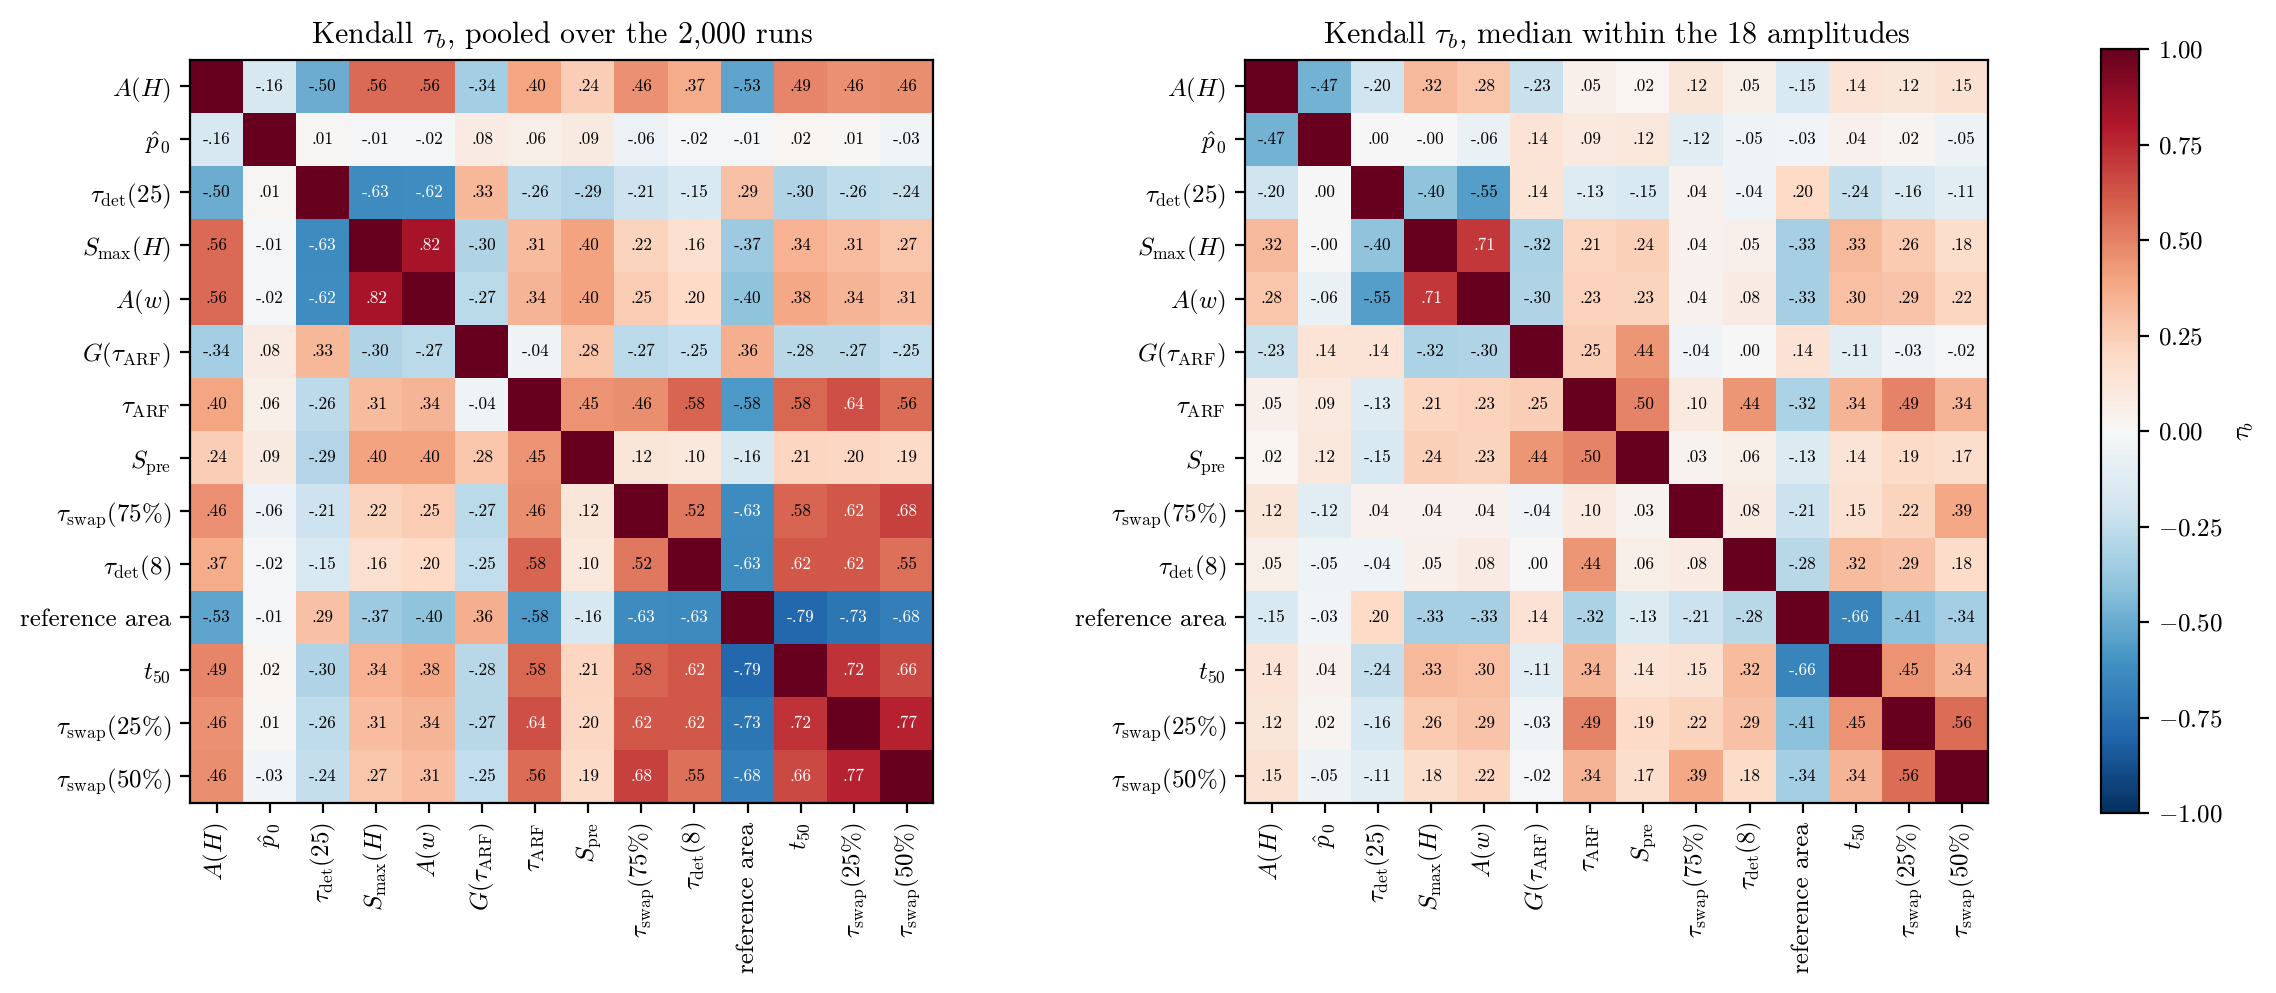
\includegraphics[width=0.86\textwidth]{Fig_QD_matrice_correlations_full.png}
  \end{center}
  \vspace{-0.5em}
  \small
  \begin{columns}[T,onlytextwidth]
    \begin{column}{0.32\textwidth}
      \textbf{Left, pooled:} almost everything agrees, because the drift size moves every
      indicator.
    \end{column}\hfill
    \begin{column}{0.32\textwidth}
      \textbf{Right, within a size:} two groups remain, \emph{evidence} ($0.71$) and
      \emph{repair}, weakly joined.
    \end{column}\hfill
    \begin{column}{0.32\textwidth}
      Best date against the analytic reference: \alert{3 trees replaced}, $0.45$, ahead of
      the first tree, $0.34$.
    \end{column}
  \end{columns}
  \note{Pour voir tous les indicateurs d'un coup, nous en avons croisé quatorze. Le panneau
    de gauche mélange tous les runs : presque tout est fortement corrélé avec tout. C'est une
    illusion, le paradoxe de Simpson : la taille du drift déplace chaque indicateur, donc le
    mélange fabrique de l'accord. Le panneau de droite calcule les mêmes corrélations à
    l'intérieur de chaque taille de drift. L'essentiel de l'accord disparaît, et deux groupes
    subsistent. Un groupe mesure la preuve et les dégâts : le pic du détecteur et l'erreur
    excédentaire sur la transition s'accordent fortement. L'autre groupe mesure la
    réparation. Entre les deux groupes, les liens restent faibles. Nous avons aussi comparé
    les dates de remplacement à une référence analytique, la précision de la forêt sur la
    région dont l'étiquette a changé. La date à laquelle trois arbres sont remplacés la suit
    mieux que le premier arbre. Cette matrice est exploratoire.}
\end{frame}

% =====================================================================
\section{III. Evidence vs threshold}
% =====================================================================

\begin{frame}{Part III --- Evidence against the threshold}
  \begin{center}\carte{3}\end{center}
  \note{La troisième partie relie les deux premières.}
\end{frame}

\begin{frame}{The race is decided before the repair}
  \begin{columns}[c,onlytextwidth]
    \begin{column}{0.52\textwidth}
      \centering
      \resizebox{\linewidth}{!}{\schemaidentite}\\
      {\scriptsize\color{gray} schematic}
    \end{column}\hfill
    \begin{column}{0.44\textwidth}
      A time counts observations; $\lambda$ counts \emph{excess errors}. Comparing them
      needs a rate that does not exist.
      \begin{block}{Race identity, on every run}
        \vspace{-0.4em}
        \[
          \tau_{\mathrm{det}} < \tau_{\mathrm{ARF}}
          \iff S_{\mathrm{pre}} \ge \lambda
        \]
        \vspace{-0.9em}
        \[
          S_{\mathrm{pre}} = \max_{t < \tau_{\mathrm{ARF}}} S_t
        \]
      \end{block}
      \vspace{-0.3em}
      {\scriptsize\color{gray} $S_{\mathrm{pre}}$: the highest the detector's evidence gets
       before the forest repairs itself\par}
      \vspace{0.3em}
      \small No rate, no averaging, no assumption on the trees. Checked on $2\,000$ runs out
      of $2\,000$ at three thresholds.
    \end{column}
  \end{columns}
  \note{Voici l'étape clé. Un temps de réparation compte des observations. Un seuil compte
    des erreurs excédentaires. Ils ne sont pas dans la même unité, et l'article fait le pont
    avec un taux moyen d'erreurs par pas. Ce taux n'existe pas : il chute à mesure que la
    forêt se répare, et le détecteur oublie sa preuve chaque fois qu'il touche zéro.
    L'énoncé exact est bien plus simple. Regardez la statistique du détecteur jusqu'au
    premier remplacement, et prenez son point le plus haut : nous l'appelons S pré. Le
    détecteur arrive premier si et seulement si S pré atteint le seuil. Avec un seuil bas, il
    est atteint avant la réparation ; avec un seuil haut, il ne l'est pas. C'est exact sur
    chaque run, ça ne demande ni taux, ni moyenne, ni hypothèse sur les arbres, et nous
    l'avons vérifié sur les deux mille runs.}
\end{frame}

\begin{frame}{The evidence before the repair sets the transition}
  \begin{columns}[c,onlytextwidth]
    \begin{column}{0.60\textwidth}
      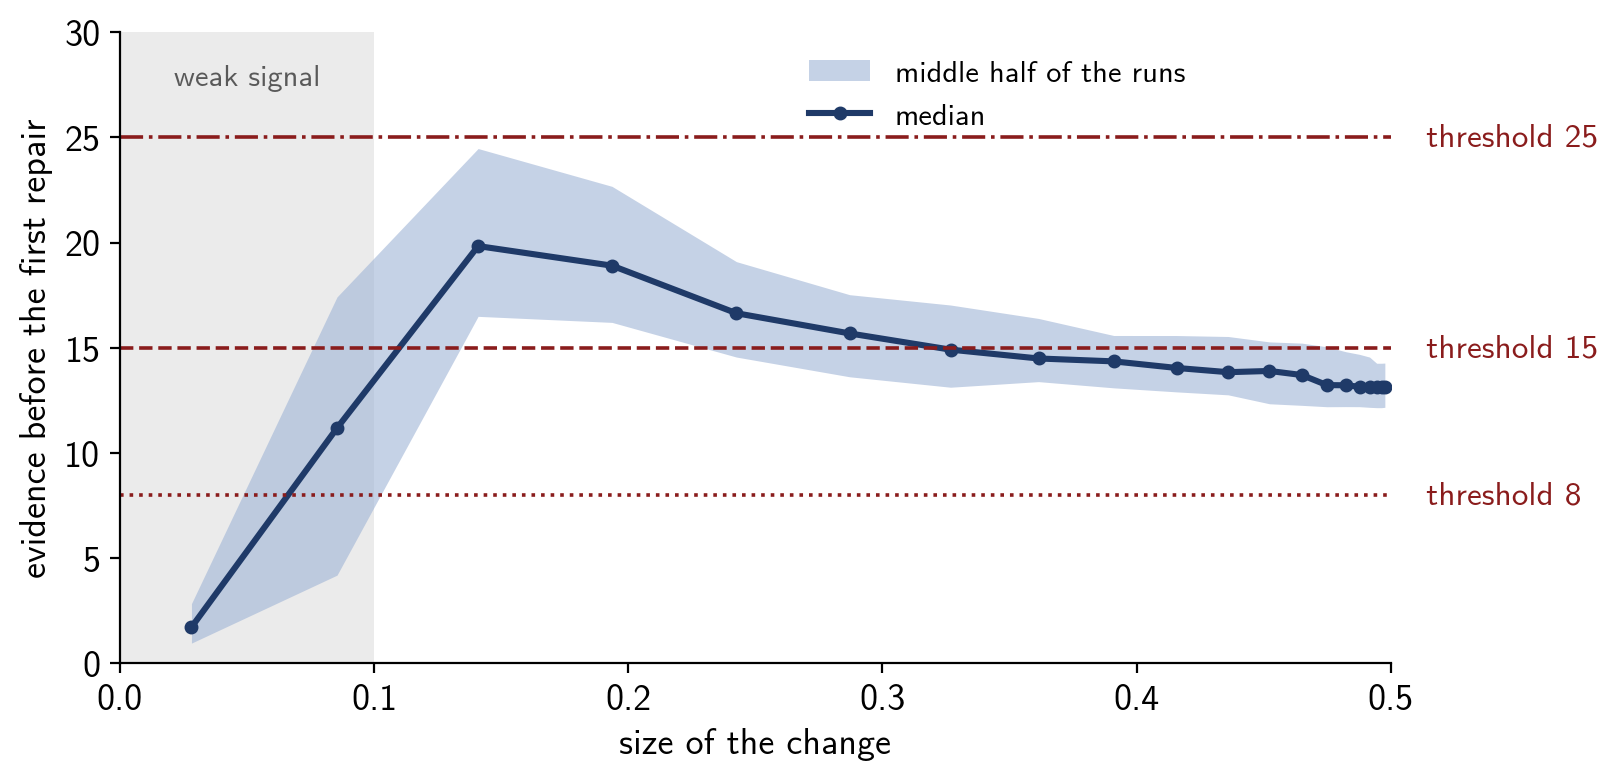
\includegraphics[width=\textwidth]{Fig_slide_spre.png}
    \end{column}\hfill
    \begin{column}{0.37\textwidth}
      \begin{itemize}
        \item Above the weak-signal zone, the median lies between \textbf{$13.1$ and $19.8$}:
              the transition the paper sees between $15$ and $25$, \alert{and leaves
              unexplained}.
        \item It \textbf{decreases} as the drift grows: at $\lambda = 15$ the detector wins
              $81\%$, then only $18\%$. That is the paradox.
      \end{itemize}
    \end{column}
  \end{columns}
  \note{Nous avons donc mesuré S pré sur chaque run. La ligne sombre est la médiane par
    taille de drift, la bande contient la moitié centrale des runs, et les lignes rouges sont
    des seuils. Au-dessus de la zone de signal faible, la médiane se situe entre treize et
    vingt. Un seuil sous ce niveau est atteint avant la réparation dans la plupart des runs ;
    un seuil au-dessus l'est rarement. C'est exactement la transition que l'article observe
    entre quinze et vingt-cinq, et qu'il laisse aux travaux futurs. Regardez maintenant la
    forme. Après les drifts moyens, S pré décroît quand le drift se renforce, parce que le
    premier remplacement vient plus tôt. À seuil fixé à quinze, le détecteur gagne
    quatre-vingt-un pour cent des courses sur les drifts moyens, et seulement dix-huit pour
    cent sur les plus forts. Le paradoxe, c'est cette preuve décroissante, lue face à un
    seuil fixe. Tout à gauche, le drift est trop faible pour accumuler quoi que ce soit :
    c'est un autre régime.}
\end{frame}

\begin{frame}{Stronger drifts leave no more evidence}
  \begin{columns}[c,onlytextwidth]
    \begin{column}{0.48\textwidth}
      \centering
      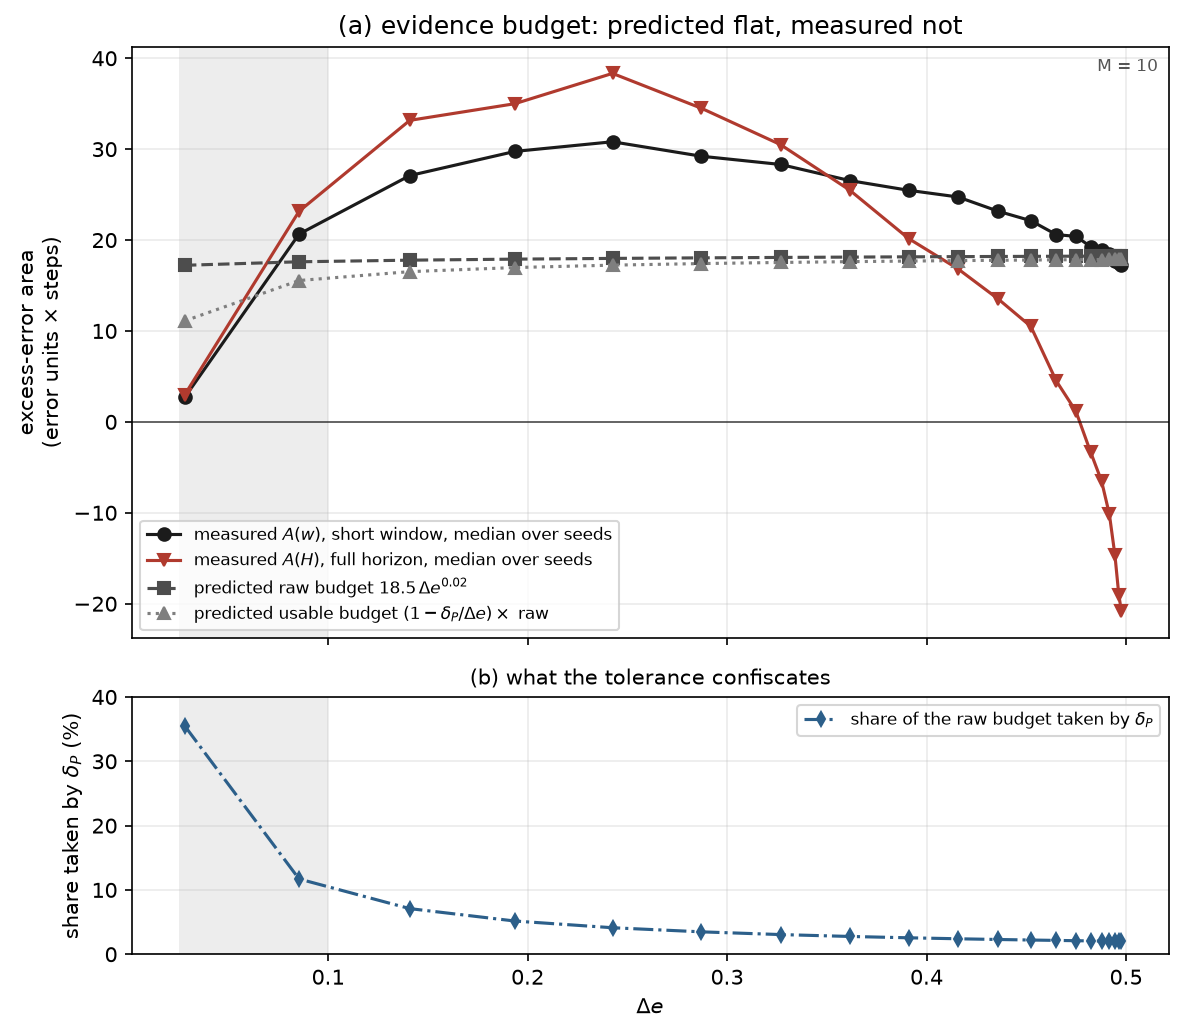
\includegraphics[height=0.66\textheight]{Fig_QC_budget_utilisable_full.png}
    \end{column}\hfill
    \begin{column}{0.46\textwidth}
      \begin{itemize}
        \item The paper's picture: an excess error $\Delta e$ over a window $\tau_{\mathrm{ARF}}$,
              so the area stays almost constant.
        \item Measured over the transition, the area varies by a factor of $1.8$ while the
              drift size varies by $5.8$: \alert{the compensation is real}.
        \item But the paper's rectangle misestimates it by up to $43\%$, and over the whole
              horizon the area turns negative at large drifts: the new task is easier.
      \end{itemize}
    \end{column}
  \end{columns}
  \note{Pourquoi un drift violent ne laisse-t-il pas plus de preuve qu'un drift doux ?
    L'image de l'article est un rectangle : une erreur excédentaire de hauteur delta e,
    pendant une fenêtre égale au temps de réparation. Comme le temps de réparation décroît
    comme un sur delta e, l'aire reste presque constante. Nous avons mesuré l'aire
    directement. Sur la transition, elle varie d'un facteur inférieur à deux, alors que la
    taille du drift varie de presque six : la compensation est réelle. Mais le rectangle
    lui-même est faux. Il se trompe sur l'aire jusqu'à quarante-trois pour cent, parce que le
    premier remplacement n'est pas la largeur du transitoire. Et sur tout l'horizon, aux
    grands drifts, l'aire devient même négative : après le changement, la tâche est plus
    facile qu'avant, et l'erreur se stabilise sous son ancien niveau. La preuve existe, elle
    est à peu près constante, mais la dérivation qu'en fait l'article ne tient pas.}
\end{frame}

\begin{frame}{Detecting is not winning}
  \begin{center}
    \begin{tabular}{@{}cccc@{}}
      \toprule
      threshold $\lambda$ & alarm fires & detector arrives first & false alarms, no drift \\
      \midrule
      $8$  & $95.3\%$ & $\mathbf{91.0\%}$ & $4.15\%$ \\
      $15$ & $92.9\%$ & $\mathbf{36.3\%}$ & $0.15\%$ \\
      $20$ & $66.2\%$ & $8.1\%$           & $0.00\%$ \\
      $25$ & $38.9\%$ & $2.5\%$           & $0.00\%$ \\
      \bottomrule
    \end{tabular}\\[0.3em]
    {\scriptsize\color{gray} $2\,000$ runs with drift and $2\,000$ without, over $2\,000$ steps}
  \end{center}
  \begin{itemize}
    \item At $\lambda = 15$ the alarm almost always fires, but mostly \emph{after} the repair.
    \item At $\lambda = 8$ the detector wins $91\%$ of races for $4.15\%$ of drift-free runs
          with a false alarm: the paper's ``no threshold escapes'' does not hold on this bench.
    \item \textcolor{gray}{Not tested: the heteroscedastic streams where the paper places its
          false-alarm tension.}
  \end{itemize}
  \note{Une conséquence pratique. Détecter un drift et gagner la course sont deux choses
    différentes. Au seuil quinze, l'alarme part sur quatre-vingt-treize pour cent des
    drifts, ce qui paraît excellent, mais elle arrive avant la réparation dans seulement
    trente-six pour cent d'entre eux. La plupart de ces alarmes viennent après que la forêt a
    déjà changé. Au seuil huit, le détecteur gagne quatre-vingt-onze pour cent des courses,
    et environ quatre pour cent des runs où rien ne se passe lèvent une fausse alarme en deux
    mille pas. Au seuil douze, il gagne encore soixante-dix-neuf pour cent des courses, pour
    un demi pour cent de fausses alarmes. Donc sur ce banc, les seuils bas échappent bel et
    bien au point aveugle, et l'affirmation de l'article qu'aucun seuil n'y échappe doit
    être restreinte. Nous n'avons pas testé les flux financiers à volatilité groupée, où
    l'article situe le problème des fausses alarmes.}
\end{frame}

% =====================================================================
\section{Conclusion}
% =====================================================================

\begin{frame}{What changes in the paper}
  \small
  \begin{tabular}{@{}p{0.34\textwidth}p{0.43\textwidth}l@{}}
    \toprule
    The paper & Our result & \\
    \midrule
    races the repair against a constant & race identified, bounded, decided run by run & \textbf{made exact} \\
    independent trees, bias asserted & direction proven, cannot reverse & \textbf{proven} \\
    error back to normal at the first replacement & it comes back later; the rectangle fails & \textbf{corrected} \\
    first replacement as the repair date & earliest date, fires without drift & \textbf{qualified} \\
    transition between $15$ and $25$, unexplained & set by the evidence before the repair & \textbf{explained} \\
    no threshold escapes & $\lambda = 8$ and $12$ do, on this bench & \textbf{restricted} \\
    \bottomrule
  \end{tabular}
  \vspace{0.6em}
  \begin{center}
    \alert{The phenomenon survives. What changes is its mechanism and its reach.}
  \end{center}
  \note{Pour résumer ce que notre travail change dans l'article. La course, qui comparait un
    temps aléatoire à une constante, est rendue exacte : identifiée, bornée, et décidée run
    par run. Le biais de l'hypothèse d'indépendance était affirmé ; il est maintenant
    prouvé, avec son sens. L'idée que l'erreur est revenue à la normale au premier
    remplacement est corrigée. Le premier remplacement comme date de réparation est
    qualifié : c'est la date la plus précoce et elle se déclenche sans drift. Le seuil de
    transition, que l'article laissait inexpliqué, est expliqué par la preuve avant la
    réparation. Et l'affirmation qu'aucun seuil n'échappe est restreinte aux réglages que
    l'article a réellement testés. Le phénomène survit à tout cela. Ce qui change, c'est son
    mécanisme, et sa portée.}
\end{frame}

\begin{frame}{An open question, and what we did not do}
  \begin{columns}[T,onlytextwidth]
    \begin{column}{0.50\textwidth}
      \begin{exampleblock}{Open: a reference for adaptation}
        Every indicator on the detector's side reads the \emph{error}, which mixes what the
        forest relearned with how hard the new task is. On analytic probes, the forest can
        relearn the changed region and lose a rare one, unseen by the error.
      \end{exampleblock}
    \end{column}\hfill
    \begin{column}{0.46\textwidth}
      \begin{block}{Not done}
        \small
        \begin{itemize}
          \item one forest size, one homoscedastic bench
          \item decision rule fixed during the analysis
          \item the independence bias has a sign, not a size
        \end{itemize}
      \end{block}
    \end{column}
  \end{columns}
  \note{Nous laissons une question ouverte. Toute mesure disponible pour le détecteur lit
    l'erreur, et l'erreur mélange deux choses : ce que la forêt a réappris, et la difficulté
    de la nouvelle tâche. Avec des sondes analytiques, des points dont nous connaissons la
    vraie étiquette, nous avons vu que la forêt peut réapprendre la région qui a changé tout
    en perdant une région rare ailleurs, et l'erreur ne voit pas cette perte. Alors quelle
    serait une vraie référence pour l'adaptation ? Nous n'avons pas la réponse. Et pour être
    honnêtes sur les limites : nous avons étudié une seule taille de forêt sur un seul banc
    simple, notre règle de décision a été fixée pendant l'analyse plutôt qu'avant, et nous
    pouvons donner le signe du biais d'indépendance mais pas sa taille.}
\end{frame}

\begin{frame}{Take-away}
  \begin{center}
    \small\alert{The blind spot is a budget of evidence, accumulated before the repair, set
    against a threshold.}
  \end{center}
  \vspace{-0.5em}
  \begin{center}\carte[0.71]{0}\end{center}
  \note{Retour à la carte. Le point aveugle est réel, et il survit à toutes les corrections.
    Mais ce n'est pas une course entre deux horloges. C'est la preuve que la forêt laisse
    passer avant sa première réparation, face à un seuil fixe. Cette seule grandeur explique
    quand le détecteur gagne, pourquoi la transition est là où elle est, et pourquoi les
    drifts plus forts sont ratés plus souvent. Merci de votre attention ; nous sommes à votre
    disposition pour vos questions.}
\end{frame}

% =====================================================================
\appendix
\section*{Backup}
% =====================================================================

\begin{frame}{Backup --- The supervisor's additional questions}
  {\small Treated in a separate working document on the same campaign; not merged into the report.}
  \begin{itemize}
    \item \textbf{Shape of the error after the drift}: not exponential, and its half-recovery comes
          \emph{after} the median first replacement on $17$ of the $18$ readable drift sizes.
          The first replacement is early, again.
    \item \textbf{End of the horizon}: the error settles \emph{below} its pre-drift baseline at all
          $20$ drift sizes. The new task is easier.
    \item \textbf{Inside the forest} (pilot, $100$ runs): disagreement between trees halves when only
          $63$ to $66\%$ of them are renewed --- the surviving trees learn too. After a strong drift,
          new trees err far less than survivors.
    \item \textbf{A z-score of the error drop} measures the number of seeds, not the dynamics.
  \end{itemize}
  \vfill
  {\small\color{gray} Open, and worth continuing: a reference for adaptation, the size of the
  independence bias, heteroscedastic streams, tree-by-tree dynamics.}
\end{frame}

\begin{frame}{Backup --- Fréchet bounds}
  For integer-valued clocks with marginal CDFs $F_A$ and $F_D$, and \emph{any} coupling,
  \begin{align*}
    P_{\mathrm{miss}} &\ge \max\Big(0,\ \sup_{s} \big[F_A(s)-F_D(s)\big]\Big),\\
    P_{\mathrm{miss}} &\le \min\Big(1,\ \inf_{s} \big[F_A(s) + 1 - F_D(s+1)\big]\Big).
  \end{align*}
  \begin{itemize}
    \item Lower: Fréchet on $\{\tau_{\mathrm{ARF}} \le s < \tau_{\mathrm{det}}\} \subseteq \mathrm{Miss}$.
    \item Upper: $\mathrm{Miss} \subseteq \{\tau_{\mathrm{ARF}} \le s\} \cup \{\tau_{\mathrm{det}} > s+1\}$, then Boole.
    \item Toy case, both clocks uniform on $\{1,2\}$: the bounds $0$ and $0.5$ are both attained.
  \end{itemize}
\end{frame}

\begin{frame}{Backup --- Lindley's closed form and the certificate}
  With $X_t = e_t - \hat p_0 - \delta_P$ and $A(k,j) = \sum_{t=k+1}^{j} (e_t - \hat p_0)$,
  \[
    S_j = \max_{0 \le k \le j} \sum_{t=k+1}^{j} X_t,
    \qquad
    S_{\max}(H) = \max_{0 \le k \le j \le H} \big[A(k,j) - (j-k)\,\delta_P\big].
  \]
  \begin{itemize}
    \item Certificate: the alarm fires by $H$ iff some sub-window carries
          $A(k,j) \ge \lambda + (j-k)\,\delta_P$. The full window alone is only sufficient.
    \item Race identity: the same maximum, taken up to the first replacement, is $S_{\mathrm{pre}}$.
  \end{itemize}
\end{frame}

\begin{frame}{Backup --- Association protocol}
  \begin{itemize}
    \item Every coefficient is computed \textbf{within a drift size} ($100$ seeds), on the $18$
          sizes with $\Delta e \ge 0.10$: pooling measures the drift size, not the link.
    \item Kendall's $\tau_b$: reads on pairs, corrects for ties. Censored durations ranked last,
          licit because the horizon is common to all runs.
    \item Pearson undefined on censored values; Spearman handles their ties implicitly.
    \item Percentile bootstrap over seeds, $2\,000$ resamples; discernible if the interval
          excludes zero. Fixed during the analysis, not before: stated in the report.
    \item Complete cases instead of ranking censored runs last: no coefficient moves by more
          than $0.0403$.
  \end{itemize}
\end{frame}

\begin{frame}{Backup --- The drift-free control}
  \begin{center}
    \begin{tabular}{@{}lr@{}}
      \toprule
      On $2\,000$ runs with no change point & \\
      \midrule
      runs where at least one tree is replaced & $2\,000/2\,000$ \\
      first replacement, median & $95$ steps \\
      distinct trees renewed, median & $9/10$ \\
      forest entirely renewed & $28.7\%$ \\
      \midrule
      first replacement at the weakest drift, median & $118$ steps \\
      \bottomrule
    \end{tabular}
  \end{center}
\end{frame}

\begin{frame}{Backup --- Notation}
  \begin{center}
    \small
    \begin{tabular}{@{}ll@{}}
      \toprule
      $\Delta e$ & drift size: the jump in error a stale model suffers \\
      $\tau_{\mathrm{ARF}}$ & first tree replaced after the change \\
      $\tau_{\mathrm{swap}}(q)$ & first time a share $q$ of the trees has been replaced \\
      $\tau_{\mathrm{det}}$ & first alarm of the external detector, possibly never \\
      $S_t$, $\lambda$ & detector statistic and its threshold \\
      $S_{\mathrm{pre}}$ & highest $S_t$ reached before the first replacement \\
      $A(w)$, $A(H)$ & excess error over the transient window, over the whole horizon \\
      $G$ & share of the detector's final evidence already reached at $\tau_{\mathrm{ARF}}$ \\
      \bottomrule
    \end{tabular}
  \end{center}
\end{frame}

\end{document}
